%--------------------PREAMBLE-------------------------
\documentclass[a4paper,11 pt,twoside, BCOR11mm]{scrbook}
%--------------------Packages-------------------------
\usepackage{latexsym}         % Fuer recht seltene Zeichen
\usepackage[utf8]{inputenc}   % =E4 =F6 =FC =DF; danach  geht auch das ß richtig
\usepackage{caption}          % Figure-Captions formatieren
%\captionsetup[subfigure]{font={sf,md,sl,small},labelfont={sf,md,sl,small}}
%\setkomafont{caption}{\itshape\sffamily}
%\setkomafont{captionlabel}{\upshape\bfseries\sffamily}
%\usepackage{sectsty}          % Section headings formatieren
\usepackage{amsmath,amsthm}
%\usepackage{fancyhdr}
\usepackage[automark, komastyle, headsepline, plainfootsepline]{scrpage2}
\usepackage{amssymb}
\usepackage{xfrac}
\usepackage{algorithm}
\usepackage{algorithmic}
\usepackage[a4paper,lmargin={2.5cm},rmargin={2.5cm},tmargin={3cm},bmargin={2.5cm}]{geometry}
\usepackage{picinpar}
\usepackage{enumitem}
\usepackage{graphicx}
\usepackage{wrapfig}
\usepackage{graphics} % for pdf, bitmapped graphics files
\usepackage{epsfig} % for postscript graphics files
\usepackage{mathptmx} % assumes new font selection scheme installed
\usepackage{times} % assumes new font selection scheme installed
\usepackage{amsmath} % assumes amsmath package installed
\usepackage{amssymb}  % assumes amsmath package installed
\usepackage{inputenc}
\usepackage[binary-units=true]{siunitx}
\DeclareSIUnit{\nothing}{\relax}
\usepackage{xcolor}
\usepackage{eqparbox}
%\usepackage{subcaption} 
\usepackage{scrhack}
\usepackage{epigraph}
\usepackage[caption=false,font=footnotesize]{subfig}
\usepackage[acronym, toc, shortcuts]{glossaries}
\usepackage{nomencl}
\usepackage{tumcolor}
%\usepackage[]{isodate}
\usepackage[backend=biber,
			style=alphabetic,
%			style=numeric,
			sorting=nyt,
			urldate=iso8601,
			date=iso8601,
			giveninits=true,
			maxbibnames=99,
			maxcitenames=99]{biblatex} 
\addbibresource{../literature/literature.bib}
\usepackage{stmaryrd} % for some symbols like \varoast (* within a circle)
\usepackage{url}
\def\UrlBreaks{\do\/\do-}
\setcounter{biburlnumpenalty}{100}
\setcounter{biburllcpenalty}{100}
\setcounter{biburlucpenalty}{100}
\usepackage[
	colorlinks=true
%	urlcolor=black,
	linkcolor=black,
%	citecolor=black
	]{hyperref}
%----------------------Data---------------------------
% TODO: everything
\newcommand{\fullname}{Florian Mirus}
\newcommand{\email}{florian.mirus@bmwgroup.com}
\newcommand{\headline}{Neuromorphic environment model for autonomous vehicle applications}
\newcommand{\thesistitle}{\headline}
\newcommand{\thesisyear}{2018}
\newcommand{\university}{Technical University Munich}
\newcommand{\matnr}{\todo}
\newcommand{\chairman}{Prof.~Dr.~Muster~Maxmann}
\newcommand{\supervisorA}{Prof.~Dr. J\"org Conradt}
\newcommand{\supervisorAuni}{Technical University Munich}
\newcommand{\supervisorB}{Prof.~Dr.~Muster~Maxmann}
\newcommand{\supervisorBuni}{Muster~University}
\newcommand{\supervisorC}{Prof.~Dr.~Muster~Maxmann}
\newcommand{\supervisorCuni}{Muster~University}
\newcommand{\mentor}{Dr.~Hans-J\"org~V\"ogel}
\newcommand{\faculty}{Department of Electrical and Computer Engineering}
\newcommand{\institute}{Neuroscientific System Theory}
\newcommand{\thday}{31st}
\newcommand{\thmonth}{October}
\newcommand{\thyear}{2018}
\newcommand{\thtype}{PhD Thesis}
\newcommand{\degree}{Doktor-Ingenieurs (Dr.-Ing.)}
\newcommand{\subdate}{31. Oktober 2018}
\newcommand{\accdate}{31. Oktober 2018}
\newcommand{\facultyger}{Fakult\"at f\"ur Elektrotechnik und Informationstechnik}
%--------------------Commands-------------------------
\newcommand\notice[1]{}
\newcommand\seppar{ \vspace{2ex} \noindent }
\newcommand{\sectionnumbering}[1]{%
  \setcounter{section}{0}%
  \renewcommand{\thesection}{\csname #1\endcsname{section}}%
}
% Command for C++
\newcommand{\CC}{C\nolinebreak\hspace{-.05em}\raisebox{.4ex}{\tiny\bf +}\nolinebreak\hspace{-.10em}\raisebox{.4ex}{\tiny\bf +}}
\def\CC{{C\nolinebreak[4]\hspace{-.05em}\raisebox{.4ex}{\tiny\bf ++}}}
% Command for dots in quotes
\newcommand*\elide{\textup{[\dots]\,}}
\makeatletter
\renewcommand{\@chapapp}{}% Not necessary...
\newenvironment{chapquote}[2][2em]
  {\setlength{\@tempdima}{#1}%
   \def\chapquote@author{#2}%
   \parshape 1 \@tempdima \dimexpr\textwidth-2\@tempdima\relax%
   \itshape}
  {\par\normalfont\hfill--\ \chapquote@author\hspace*{\@tempdima}\par\bigskip}
\makeatother
\newcommand{\abbil}[3]{#1:  #2  \longrightarrow  #3 }
\newcommand{\abb}[5]{#1:  #2  \longrightarrow  #3, #4 \longmapsto #5 }
\newcommand{\ts}{\textsuperscript}
\newcommand{\Mod}[1]{\ \mathrm{mod}\ #1}
\newcommand{\acfl}[1]{\aclp{#1} (\acsp{#1})}
\newcommand{\norm}[1]{\left\| #1 \right\|}
\newcommand*\diff{\mathop{}\!\mathrm{d}}
\newcommand*\Diff[1]{\mathop{}\!\mathrm{d^#1}}

\newtheorem{theorem}[equation]{Theorem}
\AfterEndEnvironment{theorem}{\noindent\ignorespaces}
\newtheorem{cor}[equation]{Corollary}
\AfterEndEnvironment{cor}{\noindent\ignorespaces}
\newtheorem{lemma}[equation]{Lemma}
\AfterEndEnvironment{lemma}{\noindent\ignorespaces}
\newtheorem{ex}[equation]{Example}
\AfterEndEnvironment{ex}{\noindent\ignorespaces}
\theoremstyle{definition}
\newtheorem{defn}[equation]{Definition}
\AfterEndEnvironment{defn}{\noindent\ignorespaces}
\AfterEndEnvironment{proof}{\noindent\ignorespaces}

\DeclareMathOperator{\atantwo}{atan2}

%--------------------Glossary-------------------------
\makeglossaries
%--------------------------------------------------------------------
% set glossary style
%--------------------------------------------------------------------
\setacronymstyle{short-long}
%--------------------------------------------------------------------
% actual glossary entries
%--------------------------------------------------------------------
%--------------------------------------------------------------------
% miscellaneous
%--------------------------------------------------------------------
\newacronym{NST}{NST}{Neuroscientific System Theory Group}
\newacronym[plural=GPUs, longplural=Graphics Processing Units]{GPU}{GPU}{Graphics Processing Unit}
\newacronym[plural=CPUs, longplural=Central Processing Units]{CPU}{CPU}{Central Processing Unit}
\newacronym[plural=NPUs]{NPU}{NPU}{Neuromorphic Processing Unit}
\newacronym{TUM}{TUM}{Technical University of Munich}
\newacronym{BMW}{BMW}{Bayerische Motoren Werke}
\newacronym{ABR}{ABR}{Applied Brain Research Inc.}
\newacronym{CNRG}{CNRG}{Computational Neuroscience Research Group}
\newacronym{SAE}{SAE}{Society of Automotive Engineers}
\newacronym{EU}{EU}{European Union}
\newacronym{FET}{FET}{Future Emerging Technologies}
\newacronym{ICT}{ICT}{Information and Communication Technologies}
\newacronym{CT}{CT}{Computerized Tomography}
\newacronym{MRI}{MRI}{Magnetic Resonance Imaging}
\newacronym{PC}{PC}{Personal Computer}
\newacronym{AI}{AI}{Artificial Intelligence}
\newacronym{GOFAI}{GOFAI}{Good Old-Fashioned Artificial Intelligence}
\newglossaryentry{GPS}{name={GPS}, description={\nopostdesc}}
\newacronym[parent=GPS]{CogGPS}{GPS}{General Problem Solver}   
\newacronym{ACT}{ACT}{Adaptive Control of Thought}
\newacronym{ACT-R}{ACT-R}{Adaptive Control of Thought-Rational}
\newacronym{EPIC}{EPIC}{Executive-Process/Interactive Control}
\newacronym{DDR}{DDR}{Double Data Rate}
\newacronym{SDRAM}{SDRAM}{synchronous dynamic random-access memory}
\newacronym{PROMETHEUS}{PROMETHEUS}{PROgraMme for a European Traffic of Highest Efficiency and Unprecedented Safety}
\newacronym{NAHSC}{NAHSC}{National Automated Highway System Consortium}
\newacronym{AHSRA}{AHSRA}{Advanced Cruise-Assist Highway System Research Association}
\newacronym{PReVENT}{PReVENT}{Preventive and Active Safety Application}
\newacronym{NGSIM}{NGSIM}{Next Generation Simulation}
\newacronym{HOG}{HOG}{Histogram of Oriented Gradients}
\newglossaryentry{RPM}{name={RPM}, description={\nopostdesc}}
\newacronym[parent=RPM, plural=RPMs, longplural=Raven's Progressive Matrices]{CogRPM}{RPM}{Raven's Progressive Matrix}

%--------------------------------------------------------------------
% autonomous driving / robotics
%--------------------------------------------------------------------
\newacronym[shortplural=ADAS, longplural=Advanced Driver Assistance Systems]{ADAS}{ADAS}{Advanced Driver Assistance System}
\newacronym{DATMO}{DATMO}{Detection And Tracking of Moving Objects}
\newacronym{CV}{CV}{Computer Vision}
\newacronym{LIDAR}{LIDAR}{Light Detection and Ranging}
\newacronym{RADAR}{RADAR}{Radio Detection and Ranging}
\newacronym{US}{US}{Ultrasonic Sensors}
\newacronym{DGPS}{DGPS}{Differential Global Positioning Systems}
\newacronym[parent=GPS]{SensGPS}{GPS}{Global Positioning Systems} 
\newacronym{IMU}{IMU}{Inertial Measurement Unit}
\newacronym{ACC}{ACC}{Adaptive Cruise Control}
\newacronym{SLAM}{SLAM}{Simultaneous Localization and Mapping}
\newacronym{GTSRB}{GTSRB}{German Traffic Sign Recognition Benchmark}
\newacronym{PID}{PID}{Proportional-Integral-Derivative}
\newacronym[parent=RPM]{VehRPM}{RPM}{Rotations per minute}

%--------------------------------------------------------------------
% neuromorphic projects
%--------------------------------------------------------------------
\newacronym{DARPA}{DARPA}{Defense Advanced Research Projects Agency}
\newacronym{SyNAPSE}{SyNAPSE}{Systems of Neuromorphic Adaptive Plastic Scalable Electronics}
\newacronym{FACETS}{FACETS}{Fast Analog Computing with Emergent Transient States}
\newacronym{BrainScaleS}{BrainScaleS}{Brain-inspired multiscale computation in neuromorphic hybrid systems}
\newacronym{BBP}{BBP}{Blue Brain Project}
\newacronym{HBP}{HBP}{Human Brain Project}

%--------------------------------------------------------------------
% machine learning
%--------------------------------------------------------------------
\newacronym{SVM}{SVM}{Support Vector Machine}
\newacronym{ANN}{ANN}{Artificial Neural Network}
\newacronym{HNN}{HNN}{Hardware Neural Network}
\newacronym{SNN}{SNN}{Spiking Neural Network}
\newacronym{RNN}{RNN}{Recurrent Neural Network}
\newacronym{SOM}{SOM}{Self-Organizing Map}
\newacronym{RBM}{RBM}{Resctricted Boltzmann Machine}
\newacronym{RBF}{RBF}{Radial Basis Functions Network}
\newacronym{ART}{ART}{Adaptive Resonance Theory}
\newacronym{DNN}{DNN}{Deep Neural Network}
\newacronym{CNN}{CNN}{Convolutional Neural Network}
\newacronym{FCN}{FCN}{Fully Convolutional Neural Network}
\newacronym{DBN}{DBN}{Deep Belief Network}
\newacronym{HMM}{HMM}{Hidden Markov Model}
\newacronym{HRL}{HRL}{Hughes Research Laboratories}
\newacronym{MNIST}{MNIST}{Mixed National Institute of Standards and Technology}
\newacronym{LSTM}{LSTM}{Long Short-Term Memory}
\newacronym{ReLU}{ReLU}{Rectified Linear Unit}
\newacronym{NLP}{NLP}{Natural Languange Processing}
\newacronym{CUAVE}{CUAVE}{Clemson University Audio Visual Experiments}
\newacronym{GloVe}{GloVe}{Global Vectors}
\newacronym{COCO}{MS COCO}{Microsoft Common Objects in COntext}

%--------------------------------------------------------------------
% neuromorphic hard-/software
%--------------------------------------------------------------------
\newacronym{ROLLS}{ROLLS}{Reconfigurable On-Line Learning Spiking}
\newacronym{SpiNNaker}{SpiNNaker}{Spiking Neural Network Architecture}
\newacronym{CAVIAR}{CAVIAR}{Convolution Address-Event Representation Vision Architecture for Real-Time}
\newacronym{HICANN}{HICANN}{High Input Count Analog Neural Network}
\newacronym{PyNN}{PyNN}{Python Neural Networks}
\newacronym{Nengo}{Nengo}{Neural Engineering Objects}
\newacronym{AER}{AER}{Address Event Representation}
\newacronym{DVS}{DVS}{Dynamic Vision Sensor}
\newacronym{eDVS}{eDVS}{embedded Dynamic Vision Sensor}
\newacronym{DAVIS}{DAVIS}{Dynamic and Active Pixel Vision Sensor}
\newacronym{APS}{APS}{Active Pixel Sensor}
\newacronym{DAS}{DAS}{Dynamic Audio Sensor}
\newacronym{PACMAN}{PACMAN}{Partitioning And Configuration MANager}
\newacronym{NEST}{NEST}{NEural Simulation Tool}
\newacronym{PyNCS}{PyNCS}{Python Neuromorphic Cognitive Systems}
\newacronym{STDP}{STDP}{Spike Timing Dependant Plasticity}
\newacronym{NEF}{NEF}{Neural Engineering Framework}
\newacronym{VLSI}{VLSI}{Very-Large-Scale Integration}
\newacronym{LIF}{LIF}{Leaky-Integrate-and-Fire}
\newacronym{IF}{IF}{Integrate-and-Fire}
\newacronym{Spaun}{Spaun}{Semantic Pointer Architecture Unified Network}
\newacronym{FPGA}{FPGA}{Field Programmable Gate Array}
\newacronym{CCD}{CCD}{Charge Coupled Device}
\newacronym{ASIC}{ASIC}{Application Specific Integrated Circuit}
\newacronym{ETANN}{ETANN}{Electrically Trainable Artificial Neural Network}
\newacronym{BP}{BP}{Back Propogation}
\newacronym{LEGION}{LEGION}{Local Excitatory Global Inhibitory Oscillator Network}
\newacronym{AF}{AF}{Activation Function}
\newacronym{SIMD}{SIMD}{single instruction multiple data}
\newacronym{PE}{PE}{Processing Element}
\newacronym{GP}{GP}{General Purpose}
\newacronym{SAND}{SAND}{Simple Applicable Neural Device}
\newacronym{HAGEN}{HAGEN}{Heidelberg AnaloG Evolvable Neural Network}
\newacronym{FINFET}{FinFET}{Fin Field Effect Transistor}
\newacronym{STM}{STM}{synaptic time multiplexing}
\newacronym{HNC}{HNC}{Hecht-Nielsen Neurocomputer Corporation}
\newacronym{ANC}{ANC}{Analog Network Core}
\newacronym{MOSFET}{MOSFET}{Metal Oxide Semiconductor Field Effect Transistor}
\newacronym{EEPROM}{EEPROM}{Electrically Erasable Programmable Read-Only Memory}
\newacronym{SNR}{SNR}{signal-to-noise ratio}
\newacronym[plural=VSAs, longplural=Vector Symbolic Architectures]{VSA}{VSA}{Vector Symbolic Architecture}
\newacronym{SPA}{SPA}{Semantic Pointer Architecture}
\newacronym[plural=BSCs, longplural=Binary Spatter Codes]{BSC}{BSC}{Binary Spatter Code}
\newacronym{MAP}{MAP}{Multiply-Add-Permutate}
\newacronym[plural=HRRs, longplural=Holographic Reduced Representations]{HRR}{HRR}{Holographic Reduced Representation}
\newacronym{HTM}{HTM}{Hierarchical Temporal Memory}
\newacronym[plural=SDRs, longplural=Sparse Distributed Representations]{SDR}{SDR}{Sparse Distributed Representation}
\newacronym{FLOPS}{FLOPS}{Floating Point Operations per Second}
%--------------------------------------------------------------------
% mathematics
%--------------------------------------------------------------------
\newacronym{DFT}{DFT}{Discrete Fourier Transform}
\newacronym{IDFT}{IDFT}{Inverse Discrete Fourier Transform}
\newacronym{RMSE}{RMSE}{Root-Mean-Square Error}
%--------------------------------------------------------------------
% various
%--------------------------------------------------------------------
\newacronym{TORCS}{TORCS}{The Open Racing Car Simulator}
\newacronym{PES}{PES}{Prescribed Error Sensitivity}
\newacronym{ROS}{ROS}{Robot Operating System}

%------------------Nomenclature-----------------------
\makenomenclature
\nomenclature{$\mathbb{R}$}{The field of real numbers}
\nomenclature{$\mathbb{C}$}{The field of complex numbers}
%----------------------Style--------------------------
% \sloppy % needed to avoid line overflow
%--------------TRENNUNGSLISTE-------------------------
\hyphenation{}
%-----------------------------------------------------
\allsectionsfont{\sffamily}
\captionsetup{margin=1cm,font=small,labelfont=bf}


\pagestyle{scrheadings}
\clearscrheadfoot
\setheadsepline{0.4pt}
\renewcommand{\chaptermark}[1]{\markboth{#1}{}}
\renewcommand{\sectionmark}[1]{\markright{\thesection\ #1}}
\rehead{{\bfseries\leftmark}}
\lohead{{\bfseries\rightmark}}
\lehead{{\bfseries\thepage}}
\rohead{{\bfseries\thepage}}
%TODO remov draft date in final version 
\cefoot[draft from \today]{draft from \today}
\cofoot[draft from \today]{draft from \today}

%------------------END PREAMBLE-----------------------

%--------------------DOCUMENT-------------------------
\begin{document}
%-------------------Frontmatter-----------------------
% --- Titlepage
% The title page is fully centered.
\def\titlepagebindingcor#1{\def\@titlepagebindingcor{#1}}
\def\@titlepagebindingcor{0mm}

\def\TUMLogoWidth{19mm}

% Left and right margins are exactly the same.
\def\defaultwidth{150mm}%
\def\defaulthpos{30mm + \@titlepagebindingcor}%

% Vertical positions of title page entities
\def\titlevpos{100.2mm}%
\def\informationvpos{147mm}%
\def\examinervpos{196.5mm}%
\def\datevpos{241mm}%

% --- Robustify
% check if hyperref package was loaded
%\newif\if@hyperrefloaded\@hyperrefloadedtrue
%\AtBeginDocument{%
%\@ifpackageloaded{hyperref}{%
%    \@hyperrefloadedtrue%
%  }{%
%    \@hyperrefloadedfalse%
%  }
%}

% Title Page
%\renewcommand\maketitle{%
%  % pdf links: only if hyperref was loaded in main file
%  \if@hyperrefloaded
%    \hypersetup{%
%      bookmarks    = true,         % show bookmarks bar?
%      pdftoolbar   = true,         % show Acrobat’s toolbar?
%      pdfmenubar   = true,         % show Acrobat’s menu?
%      pdffitwindow = false,        % window fit to page when opened
%      pdfstartview = {FitH},       % fits the width of the page to the window
%      pdftitle     = {\@title},    % title
%      pdfauthor    = {\@author},   % author
%      pdfsubject   = {PhD Thesis}, % subject of the document
%      pdfcreator   = {\@author},   % creator of the document
%      pdfnewwindow = true,         % links in new window
%    }%
%  \fi

\begin{titlepage}
    \if@titlepage@sansserif
      \sffamily
    \fi



    % Layouting helper
    \if@titlepage@showlayout
      % Logo box with 105% size rel. to TUM logo
      \begin{textblock*}{10.5mm}(9.75mm, 9.75mm)
          \hspace{1mm} \vspace{10.5mm}
      \end{textblock*}

      % top and bottom margin check for logo and fak text
      \begin{textblock*}{180mm}(25mm, 10mm)
          \hspace{1mm} \vspace{10mm}
      \end{textblock*}

      \begin{textblock*}{190mm}(10mm, 148.5mm) % mid
          \noindent\makebox[\hsize]{\rule{\textwidth}{1pt}}
      \end{textblock*}

      \begin{textblock*}{190mm}(10mm, 99mm) % first third
          \noindent\makebox[\hsize]{\rule{\textwidth}{1pt}}
      \end{textblock*}

      \begin{textblock*}{190mm}(10mm, 198mm) % second third
          \noindent\makebox[\hsize]{\rule{\textwidth}{1pt}}
      \end{textblock*}
    \fi



    % Logos
    % FAK logo
%    \input{inc/fak_placement.tex}
	\begin{textblock*}{10.5mm}(9.75mm + \@titlepagebindingcor, 9.75mm)
		\noindent 
\includegraphics[height = 10.5mm]{frontmatter/images/FAK_EI_RGB_s.eps}
	\end{textblock*}

    % FAK text
    %                         See TUM CD Handbook page 16
    %                         x    + x    + 0.5x
    \begin{textblock*}{120mm}(10mm + 10mm + 5mm + \@titlepagebindingcor, 13.78mm)
        \footnotesize
        \fontfamily{phv}\selectfont
        \noindent \textcolor{TUMBlue}{
          {\facultyger{}}
        }\\
        \fontfamily{phv}\selectfont
        \textcolor{TUMBlue}{
          Technische Universit\"at M\"unchen
        }
    \end{textblock*}

    % TUM logo
    \begin{textblock*}{\TUMLogoWidth}(\paperwidth - \TUMLogoWidth - 10mm, 10mm)
        \noindent 
\includegraphics[height = 10mm]{frontmatter/images/TUM_Logo_blau_rgb_s.eps}
    \end{textblock*}



    % Titel und Autor
    % Keep the name position fixed. Longer titles expand towards top.
    \begin{textblock*}{\defaultwidth}[0,1](\defaulthpos, \titlevpos)
        \centering

        {\bfseries \Large \textcolor{TUMBlue} \thesistitle{}}
%        \ifdefempty{subtitle}{}{\vspace{1ex}\bfseries\large subtitle}

        \vspace{10mm}

        {\bfseries \large \fullname{}}\\

    \end{textblock*}



    % Informationstext
    \begin{textblock*}{\defaultwidth}(\defaulthpos, \informationvpos)
        \centering
        \raggedright

        Vollst\"andiger Abdruck der von der {\facultyger{}} der Technischen
        Universit\"at M\"unchen zur Erlangung des akademischen Grades eines\\

        \vspace{6mm}

        \centering {\bfseries \large {\degree{}}}\\

        \vspace{6mm}
        \raggedright

        genehmigten Dissertation.\\

    \end{textblock*}



    % Prüfer
    \begin{textblock*}{\defaultwidth}(\defaulthpos, \examinervpos)
        \centering
        \raggedright

        \textbf{Vorsitzender:}\\
        \hspace{8mm}\hphantom{1. } \chairman{}

        \vspace{2mm}

        \textbf{Pr\"ufende der Dissertation:}\\
        \hspace{8mm}1. \supervisorA{}\\
        \vspace{0.4cm}
          %\hspace{8mm}\hphantom{2. }\supervisorAuni{}\\
        \hspace{8mm}2. \supervisorB{}\\
        \vspace{1.0cm}
          %\hspace{8mm}\hphantom{2. }\supervisorBuni{}\\
          %\hspace{8mm}3. \supervisorC{}
          %,\\\hspace{8mm}\hphantom{3. }\supervisorCuni
%


    \end{textblock*}



    % Daten
    \begin{textblock*}{\defaultwidth}(\defaulthpos, \datevpos)
        \raggedright

        Die Dissertation wurde am \subdate{} bei der Technischen Universit\"at
        M\"unchen eingereicht und durch die {\facultyger{}}
          am \accdate{}
        angenommen.

    \end{textblock*}

\end{titlepage}

% force empty page
\mbox{}
\newpage
\thispagestyle{empty}
\mbox{}
\newpage

% \setcounter{page}{1}
\thispagestyle{empty}

%% --- toc tweaking
%% Add toc itself to toc (second command)
%% AND link to the correct page (first command)
%% Without first command, the pdf link targets an empty page
%\pretocmd{\tableofcontents}{%
%	\if@openright\cleardoublepage\else\clearpage\fi
%	\phantomsection
%	\addcontentsline{toc}{chapter}{\contentsname}
%}{}{}%
%
%% Make subsubsection numbered
%\setcounter{secnumdepth}{3}
%
%% Make subsubsection appear in TOC
%\setcounter{tocdepth}{3}

\pagenumbering{roman}
\chapter*{Abstract}
\addcontentsline{toc}{chapter}{Abstract}  

The race to autonomous driving is currently one of the main forces for pushing research forward in the automotive domain.
One major reason for this development in recent years is the rapid progress of Artificial Intelligence, especially the success of deep learning, which has shown remarkable results in tasks essential for autonomous driving.
The focus of the young and emerging research field \emph{neuromorphic engineering} is on biologically inspired computing systems and algorithms, aiming to close the gap in performance and efficiency between biological and artificial computing systems.
Prototypes of neuromorphic computing hardware, although not technologically mature yet, show promise to be a useful, energy-efficient addition in future automotive applications.
However, neuromorphic computing approaches are just beginning to draw attention in the automotive domain due to these novel spiking-neuron architectures encapsulating a drastically different computing paradigm and therefore call for alternative algorithmic approaches and new programming substrates.

In this thesis, we present a first step towards a cognitive environment model for automotive applications using distributed representations and a spiking neuron substrate.
We investigate the use of vector representations, which have been previously used for problems such as cognitive modeling or natural language processing, for knowledge representation and reasoning in automotive context.
This approach to information encoding is rather generic and can be applied to various different tasks with little modifications to the representation itself.
Furthermore, such vector-based representations offer to the opportunity to be implemented in a spiking neuron substrate, which supports efficient learning algorithms and deployment on dedicated neuromorphic hardware.
This also allows us to combine the advantages of symbolization with the benefits of neural networks.
We investigate varying instantiations of our vector-based scene representation applied to different tasks.

In a first sample application, we introduce a model, that learns to classify the current driving context based on a distributed representation of the current driving scene. 
The conceptual focus here is to capture semantics of the scene allowing conclusions about the type of environment the vehicle is currently navigating, but also investigating how varying vector vocabularies and learning architectures influence task performance.
Another essential ingredient of an environment model especially in automotive context is precise knowledge about the current state and future development of all dynamic objects in the vehicle's surroundings.
We focus on the task of predicting the behavior, that is, future motion of those other traffic participants around the vehicle based on a vector-based description of the current scene using convolutive vector powers to encode spatial information.
We hypothesize, that these structured representations have the potential to capture mutual interactions between dynamically moving agents.
Prediction of other traffic participants' behavior also offers the opportunity to explore different learning approaches.
For instance, human drivers have acquired comprehension through past experience of how other cars will probably act, but adapt this knowledge continuously when encountering new situations.
From this inspiration, we learn a generic model of dynamic behavior through offline training and refine this model when perceiving behavior of a particular object through a novel mixture-of-experts model employing online learning.
To complement these more high-level reasoning tasks with a perspective on motor control, we also introduce a novel neuromorphic control architectures, that can be used to implement generic control algorithms in the language of \acp{SNN}.
This approach allows to divide larger tasks in small sub-networks combining the advantages of manual programming with neural network learning.
This allows a first impression of how future neural vehicle control based on our distributed, cognitive environment model could be achieved.

\chapter*{Zusammenfassung}
\chapter*{Acknowledgment}
\addcontentsline{toc}{chapter}{Acknowledgment}
\begin{chapquote}{Carl Friedrich Gauss}
It is not knowledge, but the act of learning, not possession but the act of getting there, which grants the greatest enjoyment
\end{chapquote}

Scientific work such as the doctoral thesis at hand would not be possible without the support of several people.
I was fortunate enough to meet a number of great people during the preparation of this thesis I would like to express my gratitude to.
First and foremost, I would like to thank my supervisor, Prof. J\"org Conradt, who gave me opportunity to work on this interesting topic while giving me the freedom to creatively explore the research area.
Furthermore, he introduced me to his \acl{NST} at Technical University of Munich, where he created an atmosphere of creativity, scientific rigor but also great camaraderie.
Randomizing the order, I would like to thank Cristian Axenie for his enthusiasm, encouragement as well as endless nights at the robot lab, Nikolai Waniek for discussions on scientific as well as any other topics of current interest, Christoph Richter for proof-reading papers as well as his pragmatic approach to research, Lukas Everding for his deadpan sense of humor and Eme\c{c} Er\c{c}elik for his help and support with organizing practical lectures at the University as well as at the BMW Summer School.
Prof. Conradt also introduced me to the neuromorphic engineering community in general and to Dr. Terry Stewart from \ac{CNRG} at University of Waterloo in particular, who also had a great impact on my doctoral research.
I would like to thank him for his continuous support across the Atlantic Ocean and for generously sharing his wide knowledge on spiking neurons, Nengo, and machine learning in general, but moreover for becoming a great mentor and role model for me.
Furthermore, I am also deeply grateful to Prof. Chris Eliasmith, the head of \ac{CNRG}, as well as Terry and all the members of \ac{CNRG} for hosting me during a six week research visit at University of Waterloo in summer 2017.
This visit not only allowed me to push my research forward thanks to the remoteness of being an ocean and a six hour time delay apart from the \enquote{usual business}.
Furthermore, I was also fortunate to meet lots of great people at University of Waterloo sharing their knowledge and experience, but I also had a great time at jam sessions or simply visiting and enjoying the beauty of Canada.
My research visit also allowed me to initiate a collaboration project between \ac{ABR}, a \ac{CNRG} spin-off company, and BMW Group with some results of that project making their way into this thesis.
As part of this collaboration project, I would like to thank Terry, Peter Blouw, Daniel Rasmussen and Eric Hunsberger on the technical side, but also Peter Suma on the administrative side for fighting with me through the pain of paperwork to make the project actually work.

I am also deeply thankful to Dr. Hans-J\"org V\"ogel, my supervisor at BMW Group, for giving me the opportunity to pursue my Ph.D. in the environment of BMW's research department.
Furthermore, he always supported and advised me with scientific and administrative tasks, defended the idea of applying neuromorphic computing \enquote{in a car} within the company and always had an \enquote{open door}, whenever something unexpected occurred.
I would also like to thank Martin Arend, the leader of my department for the most time during my Ph.D. years at BMW Group for being the nicest boss a Ph.D. student could hope for and furthermore, for not only supporting my research visit to Canada, but also joining for a couple of days and giving me the opportunity to accompany him when meeting the local start-up scene.
Another great part of pursuing my doctoral studies at BMW Group, was the network of fellow Ph.D. students within BMW's ProMotion program.
Meeting and talking to other students with similar tasks, success stories but also problems and frustrations helped me to overcome these usual but unpleasant parts of doctoral studies when progress stagnated.
In particular, I would like to express my gratitude towards Leopold Walkling and Julian Tatsch for sharing their knowledge, experience and data sets.
Furthermore, I would like to thank the \enquote{Improve} group (in no particular order): Franziska Hertlein, Sascha Steyer, Nicola Hupp, Florian Roider, Jens Schulz, Marc Vogt, Daniel Knobloch, Alexander Terres, Jan Korus, Julius Riedelbauch, Michael Ponnath, Peter R\"osch, Philip Kotter and Annette B\"ohmer.
I would also like to thank my fellow Ph.D. students at our department LT-3 Maike Hartstern and Christoph Segler for sharing the ups and downs of a Ph.D. at BMW in general and at LT-3 in particular as well as interesting scientific and daily-life discussions.
Particularly, I would like to thank Christoph for our shared efforts regarding the \enquote{management} of the dev-box as well as remembering literally every single administrative problem one could run into at BMW and, more importantly, its solution.
I would also like to express my gratitude to a couple of \enquote{regular} BMW colleagues for giving feedback to papers, talks or slides, helping out with administrative issues, interesting lunch-break discussions or simply for being great colleagues.
Again, randomizing the order, I would like to thank Mohsen Kaboli, Tom Hubregtsen, Sebastian Wirkert, Fridolin Bauer, Nadine Stockinger and Suomy Jacob. 
Additionally, I would like to thank Angelika Sch\"afer and Simone Barnloher as well as Susanne Schneider for their help and patience regarding administrative tasks related to business trips at BMW or student supervision at TUM respectively.
Finally, I would like to thank all the students I had the pleasure to supervise either at BMW or at TUM doing master or bachelor theses, project practicals, scientific seminars or simply lectures.
I hope they have learned as much from me as I learned from them.

I am also deeply thankful to my parents, Rainer and Ingrid Mirus, for being a constant source of support and encouragement when things do not work as originally planned and for providing a basement to partly finish writing of this thesis.
Thank you for supporting my life-long journey from the first steps up until this point and beyond.
Furthermore, I would like to express my gratitude to Helga Wallitzer, my mother-in-law, especially for her support during the first weeks after the birth of our daughter Isabella, which allowed me to find some sleep and get at least some work done during that great yet stressful time.
Last but not least, I would like to express the most heartfelt gratitude to my lovely wife Lisa for being on my side ever since I made the decision to move to Munich for the Ph.D., enduring my temper during the frustrating times, supporting me selflessly in everything that I do and for making me the greatest gift in the world: our daughter Isabella.
I could not have finished this thesis without you.
Thank you for everything! 

\vspace{1cm}
\fullname\\
Munich, September 2019

\renewcommand{\contentsname}{Table of Contents}
\addtocontents{toc}{\protect\setcounter{tocdepth}{-1}}
\tableofcontents
\addcontentsline{toc}{chapter}{Table of Contents}
\addtocontents{toc}{\protect\setcounter{tocdepth}{2}}
\cleardoublepage
% \setcounter{page}{1}

\phantomsection
\printglossary[title=List of Abbreviations, type=\acronymtype, style=treenoname]

\cleardoublepage
\phantomsection
\renewcommand{\nomname}{Conventions}
\addcontentsline{toc}{chapter}{Conventions}
\printnomenclature

%\cleardoublepage
%\phantomsection
%\todototoc
%\listoftodos

\cleardoublepage
%\phantomsection
%\addcontentsline{toc}{chapter}{List of Figures}
\listoffigures

\cleardoublepage
%\phantomsection
%\addcontentsline{toc}{chapter}{List of Tables}
\listoftables

%\cleardoublepage
%\phantomsection
%\addcontentsline{toc}{chapter}{List of Algorithms}
%\listofalgorithms

\cleardoublepage

\pagenumbering{arabic}
%--------------------Chapters-------------------------
\chapter{Introduction}%
\label{chap:introduction}

\section{Preamble}%
\label{sec:preamble}

The race to autonomous driving is currently one of the main forces pushing research forward in the automotive domain.
With highly automated vehicle prototypes gradually making their way to our public roads and fully-automated driving on the horizon, it seems to be a matter of time until we see robot taxis or cars navigating us through urban traffic or heavy stop-and-go on highways.
One major reason for this development in recent years is the rapid progress of \ac{AI}, especially the success of deep learning, which has shown remarkable results in tasks essential for autonomous driving such as object detection, classification \parencite{Ciresan2012} and control \parencite{Bojarski2016}.
Although more and larger data sets \parencite{Geiger2013a, Cordts2016} become available and powerful, parallel computing hardware like \acp{GPU} facilitates training of increasingly deep network architectures \parencite{Simonyan2014}, power consumption remains a critical issue.
Especially in the automotive domain as a mobile application, energy-efficiency is of crucial importance.
Furthermore, current automated vehicle prototypes rely on a rich setup of redundant sensory systems to perceive sufficient information about the outside world \parencite{Aeberhard2015}.
These sensor setups are estimated and expected to grow even further with increasing level of automation of future vehicles.
In contrast, human drivers are capable of handling challenging driving situations under changing environmental conditions by using mainly the human eyes as primary sensor input and the brain for information processing.
Furthermore, the human brain is also comparably small and efficient consuming only \SI{20}{\watt} of power, which is equivalent to a compact fluorescent light bulb, while comprising only \SI{2}{\percent} of the body weight \parencite[Chap. 2.1]{Eliasmith2013}.
Therefore, the focus of the young and emerging research field neuromorphic engineering is on biologically inspired computing systems and algorithms, aiming to close the gap in performance and efficiency between biological and artificial computing systems.
With researchers expecting a growing discrepancy between the energy and efficiency requirements of future applications, e.g., see Fig.~\ref{fig:energy_efficiency_issues} as well as \textcite{Marr2013, Farahini2016, Akopyan2015}, the demand for alternative approaches regarding computing hardware and algorithms is likely to increase.
\begin{figure}[h!]
    \centering
    \resizebox{.9\textwidth}{!}{%
        \subfloat[\label{subfig:Synapse_plot_machine_vs_environmental_complexity}]{%
            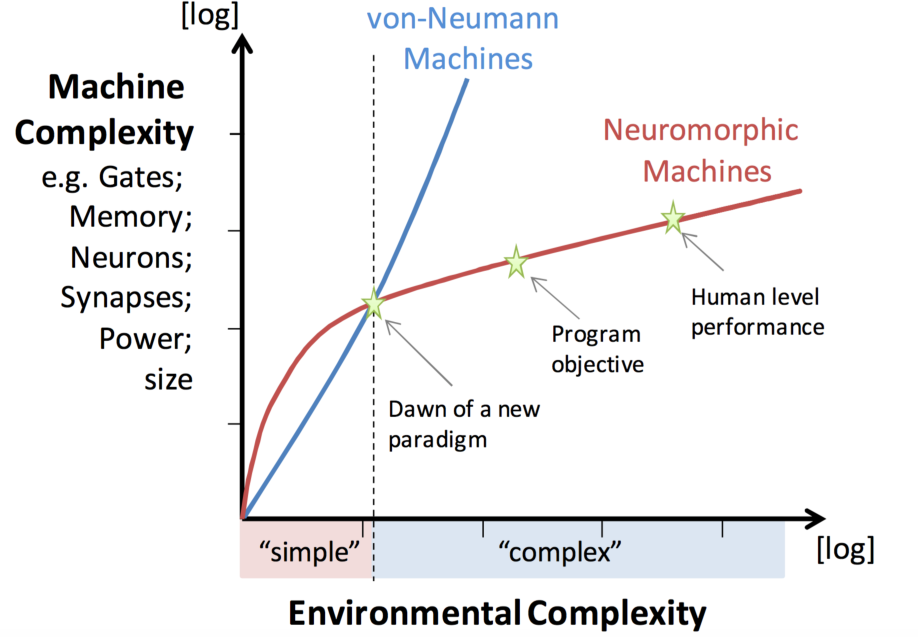
\includegraphics[height=3cm]{imgs/Synapse_plot_machine_vs_environmental_complexity.png}
        }
        \subfloat[\label{subfig:Marr_energy_eff_wall}]{%
            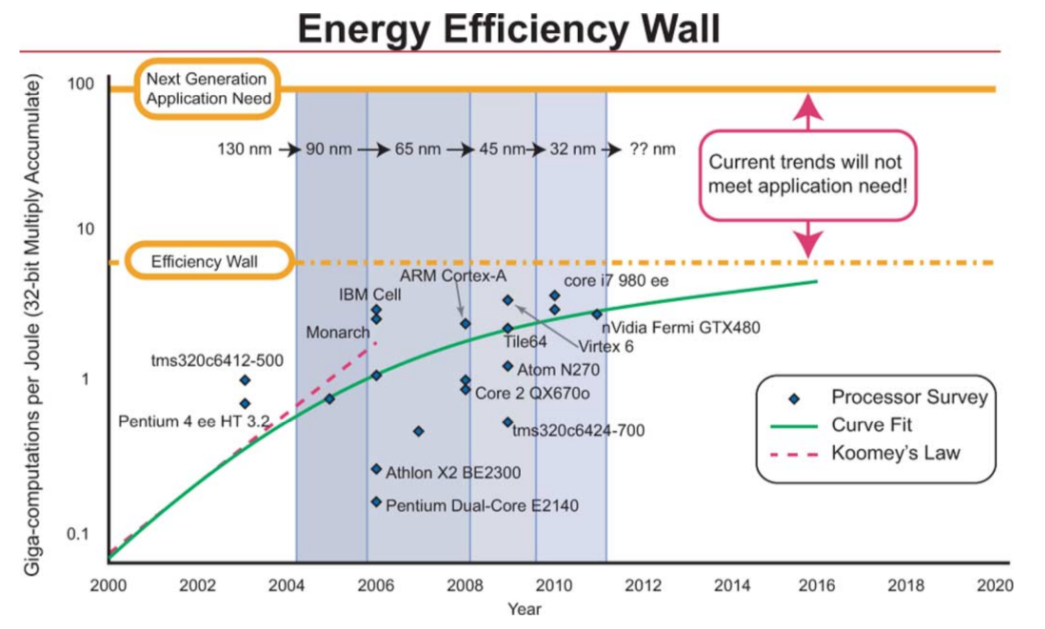
\includegraphics[height=3cm]{imgs/Marr_energy_eff_wall.png}
        }
    }
    \caption{Expected discrepancy between energy-efficiency requirements of future applications and the development of computing hardware.~\protect\subref{subfig:Synapse_plot_machine_vs_environmental_complexity} Image source: \textcite{Farahini2016}, adapted from the \acs{DARPA} \acs{SyNAPSE} program.~\protect\subref{subfig:Marr_energy_eff_wall} Image source: \textcite{Marr2013}.}
    \label{fig:energy_efficiency_issues}
\end{figure}
Although the neuromorphic prototypes of computing hardware such as \ac{SpiNNaker} \parencite{Furber2014} or  IBM's TrueNorth \parencite{Akopyan2015} dedicated to processing so-called \acp{SNN} are not technologically mature nor available as commercial products yet, they show promise to be a useful addition in future automotive applications.
Since these novel spiking-neuron architectures encapsulate a drastically different computing paradigm compared to the conventional von-Neumann architecture \parencite{vonNeumann1993}, they also call for alternative algorithmic approaches and new programming substrates \parencite{Amir2013}.

In this thesis, we investigate potential applications of neuromorphic approaches in automotive context.
Given the complexity of driving a car autonomously in all possible real-world situations, tackling the complete set of all necessary tasks is out of scope of a single thesis.
Therefore, we need to focus on certain sub-tasks.
Regarding this selection process, we contemplate two concepts.
We categorize tasks necessary for highly automated driving using the perception-action-cycle and rate their level of complexity using Moravec's paradox \parencite{Moravec1988}.
Moracev's paradox postulates the observation, that tasks or skills that seem effortless to humans are harder to reverse-engineer than tasks we experience or expect to be difficult.
Moracev argues, that we learned those seemingly effortless skills over billions of years of evolution through experience about the nature of the world such that they became unconscious to us.
A good example of this paradox is the fact that artificial systems are already able to defeat the world's best human players in games like Chess \parencite{Hsu2002} or Go \parencite{Silver2016}, which are considered particularly difficult by humans.
On the other hand, we are still struggling to create robots that solve seemingly effortless sensorimotor tasks like climbing stairs or opening doors \parencite{Guizzo2015, Norton2017}.

The perception-action-cycle \parencite{Fuster2004} is the concept of a circular flow of information between an organism or agent (living or artificial) when interacting with its environment through goal-directed behavior (Fig.~\ref{fig:perc-act-cicle}).
\begin{figure}[t!]
	\centering
	%	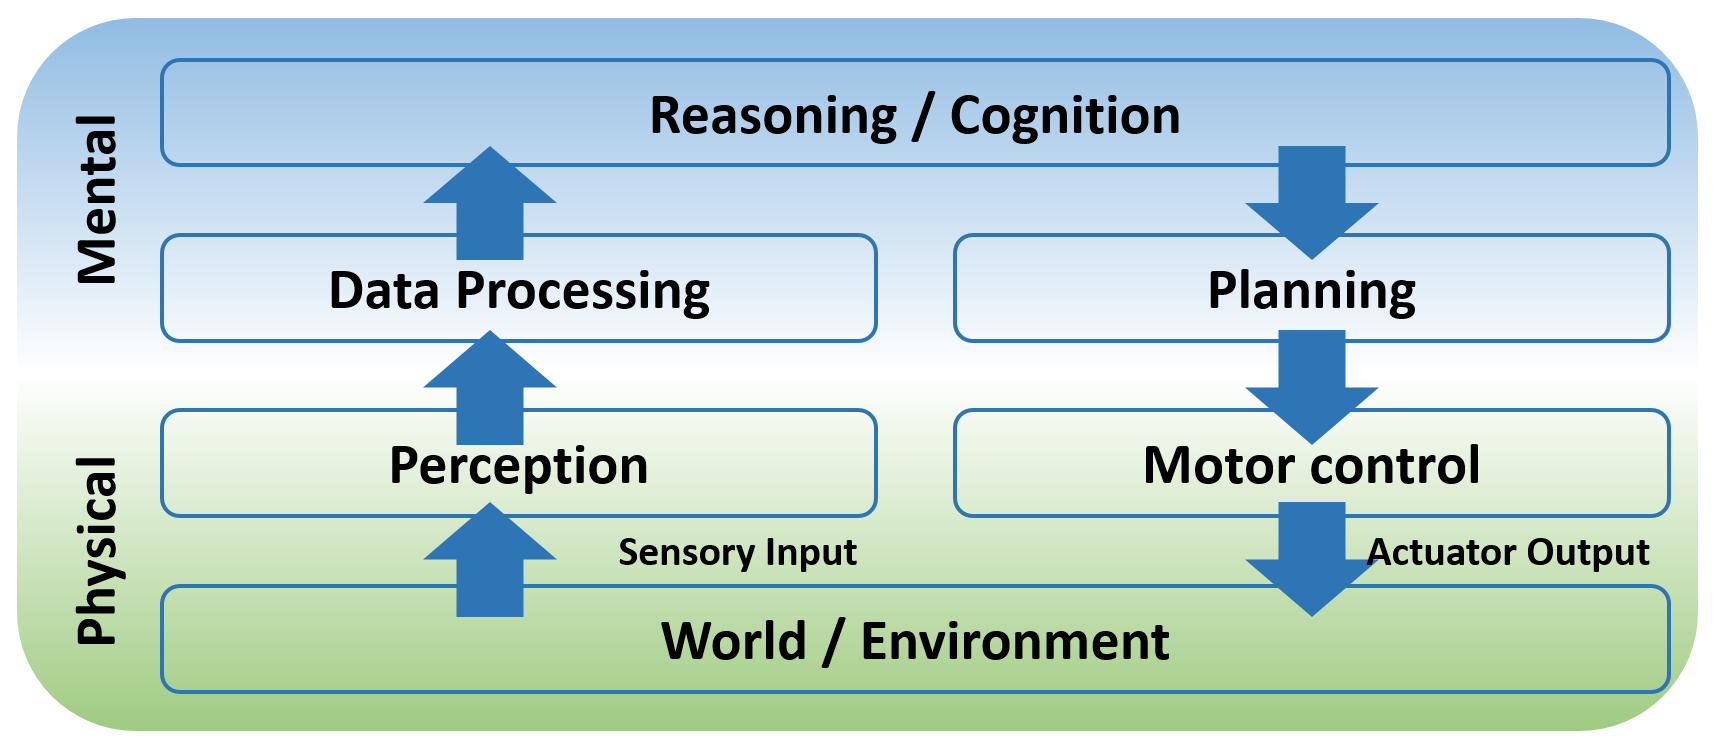
\includegraphics[width=0.85\textwidth, height=150px]{imgs/ActionPerceptionCycle.eps}
	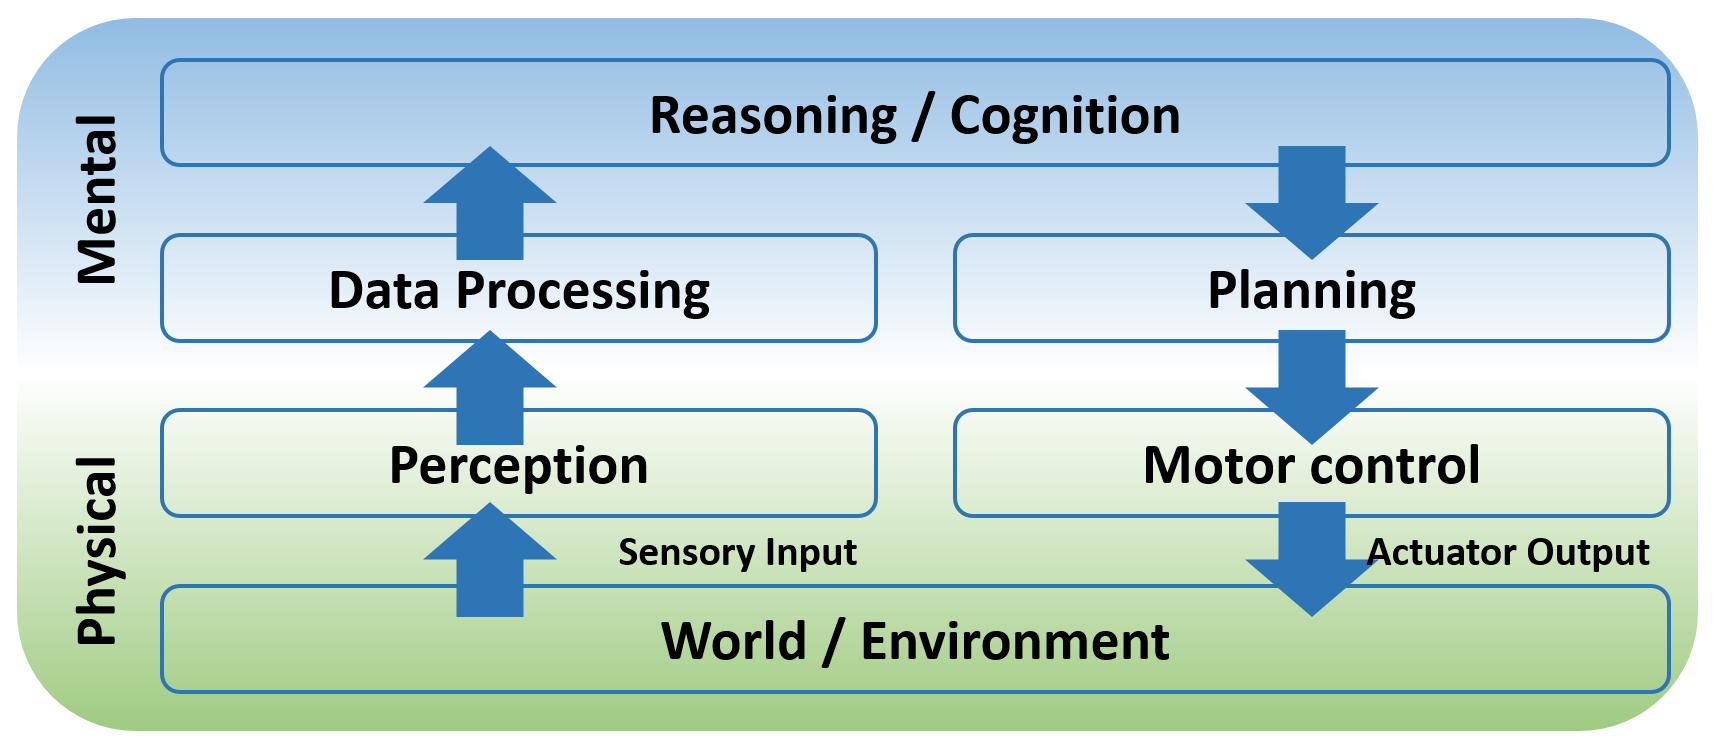
\includegraphics[width=0.85\textwidth]{imgs/ActionPerceptionCycle.eps}
	\caption{Schematic visualization of the perception-action-cycle}
	\label{fig:perc-act-cicle}
\end{figure}
Instead of considering the directional aspects of the cycle in the opposite categories of perception and action, it is also common to separate tasks in terms of hierarchy \parencite{Loeb2014}.
Interaction with the physical world through sensing and manipulation is considered on a lower hierarchical level within the perception-action-cycle while formation of mental representations and reasoning about them reside on a higher level.
We refer to those different hierarchical levels as \emph{physical} and \emph{mental} or \emph{lower} and \emph{upper} interchangeably.

Considering the physical/lower level of the perception-action-cycle, \acp{DNN} have recently shown significant progress and success at perception tasks like object detection and classification.
Therefore, we believe a lot more research is necessary until neuromorphic approaches using \acp{SNN} are sufficiently mature to compete with those traditional approaches, although current work in this directions shows promising results \parencite{Hunsberger2015}.
Similar arguments hold true for automated learning approaches regarding vehicle control.
Although sophisticated learning techniques show promise to improve motor control, to date most controllers for automated vehicles or robots in general are \enquote{designed and tuned by human engineers} \parencite{Deisenroth2013}.
One of the main reasons is the fact that control of an automated vehicle is an extremely safety-critical domain, while at the same time machine learning approaches in general pose additional challenges regarding safety validation \parencite{Koopman2016}.
Furthermore, those tasks on the physical level of the perception-action-cycle are solved effortlessly by humans and therefore, according to Moravec's paradox, we should expect them to be hard to master for artificial learning systems.
Therefore, we decided to focus on the mental/upper part of the perception-action-cycle in this thesis.
On the one hand, we believe that tasks in this part of the cycle show promise to benefit most from neuromorphic approaches.
On the other hand, \enquote{mental} tasks do not necessarily need to be performed and evaluated in closed-loop systems, which make them less problematic regarding safety issues, and therefore ideal candidates for further investigations.
It should be clear however, that \enquote{perception/action and higher level cognition are not two independent parts of one systems, but rather two integrated aspects of cognitive beings such as as ourselves} \parencite{Eliasmith2013}.
Current artificial systems are still far away from integrating both aspects effectively and more research will be necessary to close this gap.

Returning to the application domain of automated driving, precise knowledge about the current state of the environment is essential for autonomous agents and biological organisms alike to plan a secure path for navigation and to safely interact with the world.
In case of highly automated vehicles, perception of the outside world usually happens through a variety of different sensor systems such as cameras, \acs{RADAR} and \acs{LIDAR} sensors \parencite{Aeberhard2015}.
This observed information needs to be collected and combined into a central environment model, which is the (mental) basis for further reasoning and decision making.
One essential ingredient for such a model of the environment, or mental tasks in general, is knowledge or information representation.
It is an open research question to date, how the human brain represents knowledge and what underlying neural or computational substrate it uses to encode information \parencite{Wang2003, Samsonovich2012, Handjaras2016}.
Most modern approaches to reasoning or cognitive tasks in context of robotics or automated driving are built upon Bayesian probability theory and use \enquote{computer-scientific} approaches to knowledge representation.
This could be lists of objects (cf.~Fig.~\ref{subfig:urban_object_lists}) with a numerical encoding of properties when working on a higher level of abstraction.
On a lower level, another common approach especially in context of neural-network learning is to label raw sensory data, for example individual pixels of images (cf.~Fig.~\ref{subfig:urban_semantic_labels}).
However, when we as humans observe a particular scene (e.g., while driving), our mental representation will probably be very different from those aforementioned approaches.
\begin{figure}[t!]
	\centering
	\subfloat[Urban traffic scenario\label{subfig:urban_scene}]{%
		\includegraphics[width=0.45\textwidth]{imgs/urban_scene.eps}
	}
	\subfloat[Pixel-wise labels\label{subfig:urban_semantic_labels}]{%
		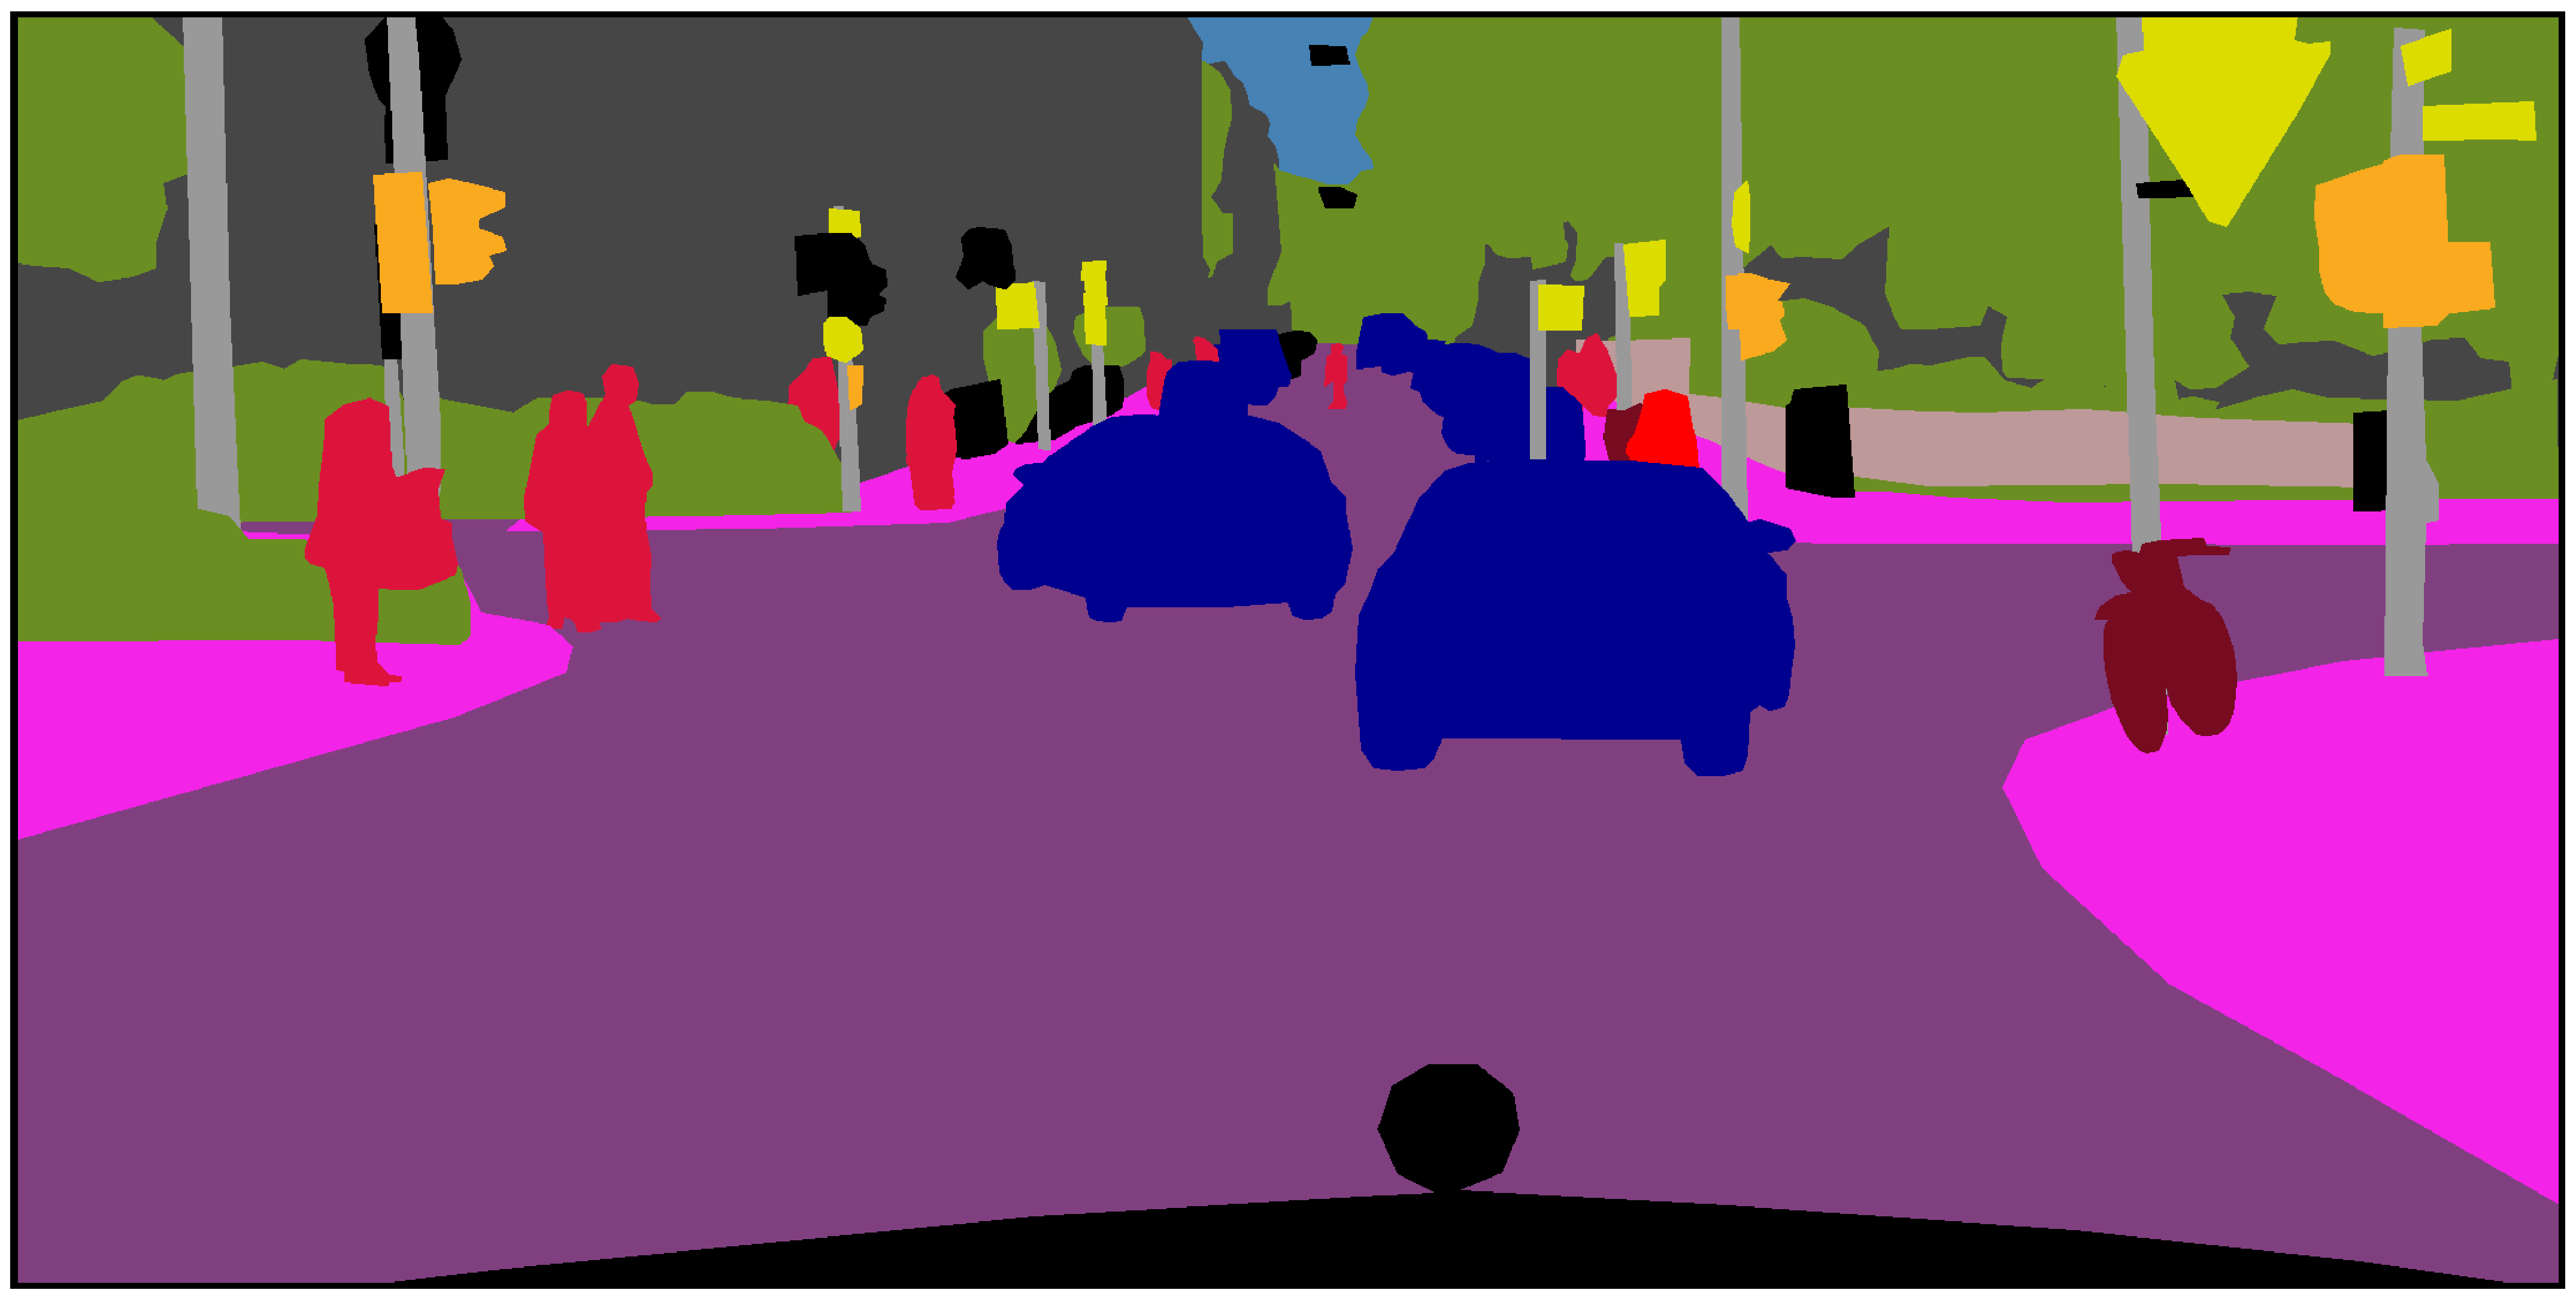
\includegraphics[width=0.45\textwidth]{imgs/urban_scene_pixel_labels.eps}
	}\\
	\subfloat[Bounding boxes indicating objects of interest\label{subfig:urban_scene_boxes}]{%
		\includegraphics[width=0.45\textwidth]{imgs/urban_scene_bound_boxes.eps}
	}
	\subfloat[Exemplary representation using lists of objects\label{subfig:urban_object_lists}]{%
		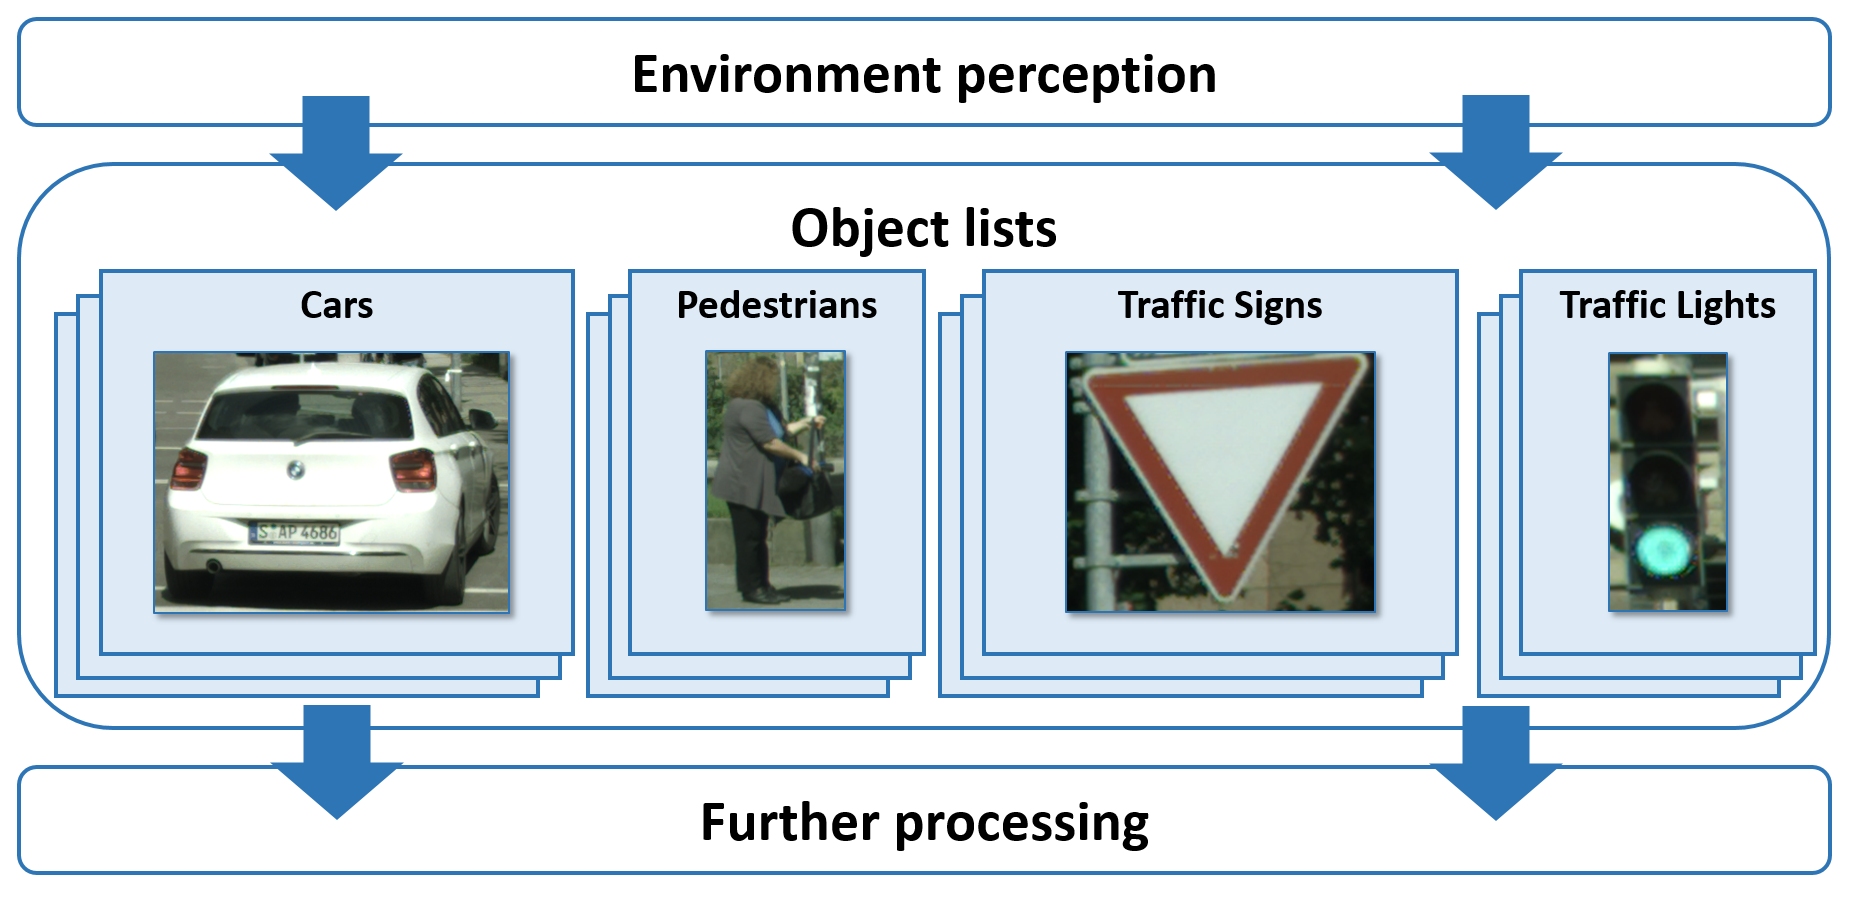
\includegraphics[width=0.45\textwidth, height=3.6cm]{imgs/urban_scene_object_lists.eps}
	}
	\caption{Example of urban driving scene with different approaches to representation. Images \ref{subfig:urban_scene}, \ref{subfig:urban_semantic_labels} and \ref{subfig:urban_scene_boxes} are (adapted) from the Cityscapes data set \parencite{Cordts2016}.}
    \label{fig:urban_scene}
\end{figure}
A human observer's representation/description of Fig.~\ref{subfig:urban_scene} would probably be in a semantic/linguistic form, for instance \emph{a blue car turning left, a white car turning right, three pedestrians waiting on the left side of the road, green traffic lights, a yield way sign}.
One common approach to encode such conceptual, semantic information or, more generally, natural language in computer-readable fashion is by using vector representations.
\acfp{VSA} is a term coined by \textcite{Gayler2003} to cover this family of modeling approaches that represent symbols or structures by mapping them to (high-dimensional) vectors.

In this thesis, we present a first step towards a cognitive environment model for automotive applications using distributed representations.
We investigate the use of these vector representations for knowledge representation and reasoning in automotive context.
This approach to information encoding is rather generic and can be applied to various different tasks with little modifications to the representation itself.
Furthermore, \acp{VSA} offer the opportunity to be implemented in a spiking neuron substrate \parencite{Eliasmith2013}, which support efficient learning algorithms and deployment on dedicated neuromorphic hardware.
This allows us to combine the advantages of symbolization with the benefits of neural networks.
We investigate varying instantiations of our representation applied to different tasks.
In a first sample application, we introduce a model learning to classify the current driving context based on a distributed representation of the current driving scene. 
The conceptual focus here is to capture semantics of the scene allowing conclusions about the type of environment the vehicle is currently navigating.
Another essential ingredient of an environment model especially in automotive context is precise knowledge about the current state and future development of all dynamic objects in the ego-vehicle's surroundings.
We focus on the task of predicting the behavior of those other traffic participants around the ego-vehicle based on a vector description of the current scene.
We hypothesize, that these structured representation have the potential to capture mutual interactions between dynamically moving agents.
Prediction of other traffic participants behavior also offers the opportunity to explore different learning approaches.
Human drivers have acquired comprehension through past experience of how other cars will probably act, but adapt this knowledge continuously when encountering new situations.
From this inspiration, we learn a generic model of dynamic behavior through offline (i.e., batch) training and refine this model when perceiving behavior of a particular object through online learning.
To complement the more high-level reasoning tasks with a perspective on motor control, we also introduce a novel neuromorphic control architecture, that can be used to implement generic control algorithms in the language of \acp{SNN}.
This approach allows to divide larger tasks in small sub-networks combining the advantages of manual programming with neural network learning.

\section{Outline of the thesis}%
\label{sec:outline_of_the_thesis}

This section provides a brief overview of the thesis structure as well as a short summary for each chapter.
Chapter~\ref{chap:research_context} summarizes the state-of-the-art in several areas related to the core of the thesis at hand spanning from biologically inspired hardware and software over cognitive modeling techniques to automated driving research.
We give an overview over all of these sub-topics providing a detailed description where necessary while putting these details in context of a bigger picture.

Chapter~\ref{chap:introduction_to_vsas} introduces the key ingredients for the models developed in later chapters, distributed representations and \acp{SNN}, and establishes the mathematical apparatus and the essential theoretical properties of these ingredients.
After proposing a more rigorous mathematical formalism to describe the general theory of \acp{VSA}, we proceed to the \ac{SPA} as a special case of \acp{VSA} with additional features and theory to be presented.
Furthermore, we give an introduction to the general ideas for cognitive modeling based on \acp{VSA} like vocabularies and structured representation generation.
Furthermore, we present a brief description of the \ac{NEF} and how it can be used to implement cognitive architectures based on vector representations in a spiking neuron substrate.

In chapter~\ref{chap:a_cognitive_approach_to_represent_automotive_scenes}, we proceed to present the general approach to encode automotive scenes in semantic vectors as representational substrate.
We show different approaches to generate vector vocabularies, which are the basic ingredients to built more complex, structured representations from.
We demonstrate successful embedding of several similarity structures into vector vocabularies designed for automotive applications.
Additionally, we present several approaches to representing numerical values in our vector substrate introducing a novel approach based on a convolutive power, generalizing exponentiation to circular convolution.
We conclude the chapter with a thorough analysis regarding the systematic limitations regarding the vectors' capacity, i.e., amount of information such vector representations can effectively store.

Chapter~\ref{chap:driving_context_classification} introduces the first sample instantiation of our vector representation applied to the task of driving context classification based on a scene vector encapsulating the current driving situation.
We establish the vector-based scene representation for the context classification task and use it as input data to a learning model implemented in a spiking neuron substrate.
To evaluate the model's performance, we present several reference learning systems using either the vector representation or visual information as input and compare them to human level performance.
Finally, we analyze the influence of the underlying vocabularies encoding different similarity structures on the learning model's classification performance.
All evaluations are conducted using real-world driving data.

In chapter~\ref{chap:behav_pred}, we introduce a second instantiation of our scene representation to predict the behavior of other objects in the vehicle's surroundings.
In the context of vehicle trajectory prediction, we employ our novel approach to encode spatial information in distributed representations to encode the positions of several vehicles in vectors of fixed length.
We employ neural networks built from \ac{LSTM} units as well as simpler single-layer \acp{SNN} to predict vehicle trajectories based on past motion.
We analyze the influence of hyperparameters, information provided to the models as well as the composition of the training data on the models' prediction accuracy.
Furthermore, we compare the models with respect to situations in which one particular model outperforms the others.
Finally, we show that it is generally possible to detect abnormal samples indicating potentially dangerous situation based solely on the distributed vector representation and unsupervised learning.
The evaluation conducted in the chapter uses data from two different data sets containing real-world driving data.

Chapter~\ref{chap:mix_online_learning} introduces an extension of the proposed trajectory prediction models for online adaptation through incremental learning.
Building on the findings in chapter~\ref{chap:behav_pred}, we present a novel mixture-of-experts model implemented in a spiking neuron substrate meant to be trained at run time to improve the prediction performance over several individual predictors.
One of the strengths of this model is that, instead of having to start from a completely blank state, it relies on several expert models, which have been previously trained and validated offline.
This model, like all models making predictions about the future, faces the issue that the actual motion of the predicted vehicle needed to compare the model's anticipated values to is future data and thus not available at the time the model actually makes its predictions.
To avoid potentially long delays in the online learning process, we propose a novel approach to spread the error signal of earlier predictions over later predictions.
Revisiting the data sets used in chapter~\ref{chap:behav_pred}, we evaluate two different variants of the mixture models adapting their weights either solely based on the prediction error or the current context of the scene.
We show, that our online learning model is able to improve over the individual predictors already after being exposed to a small set of example vehicles.

Chapter~\ref{chap:closed_loop_neuromorphic_control_systems} presents a first step towards a neuromorphic control architecture by developing two sample instantiations of neurally-inspired control algorithms.
We establish neuromorphic control architectures, that can be used to implement generic control algorithms in the language of \acp{SNN} with the advantage, that the overall task can be divided into several sub-networks.
This approach allows us to combine manual programming with the advantages of neural network learning.
Manually programmed sub-tasks can either complement learning networks within the system or serve as an initial approximation of the desired function, which allows more directed learning to improve task performance avoiding the need to start learning from a completely blank state.
As mentioned earlier, control of an automated vehicle is an extremely safety-critical application.
Hence, we present two sample applications in simplified setups: one on mobile robot manipulation demonstrating initial manual programming of a non-trivial robotic task in a spiking neuron substrate and one on vehicle trajectory control demonstrating how manually programmed modules can be complemented by learning networks.

Chapter~\ref{chap:discussion} summarizes the work and interprets the results achieved in this thesis.
We discuss the main advantages of the representations and models proposed in this work while also addressing limitations indicated by either systematic or experimental analysis.
We conclude the thesis by proposing a series of extensions and improvements, which potentially contribute to adopting the principles investigated in this thesis on a wider scale to obtain a more mature representation framework for automotive applications.

\section{Contributions of and to this thesis}%
\label{sec:contributions_of_and_to_this_thesis}

This thesis presents a first step towards a cognitive environment model for automated vehicles and thereby provides a novel perspective to knowledge representation in automotive context.
The two key ingredients for our approach are distributed representations and \acp{SNN}, which in combination offer a promising modeling substrate for cognitive tasks as shown in \textcite{Eliasmith2013, Eliasmith2012}. 
The possibility to implement distributed representations in a spiking neuron substrate offers the potential to combine symbol-like processing with the strengths of neural network learning.
Additionally, \acp{SNN} are one option to tackle increasing energy-efficiency requirements in future automated vehicles equipped with a plethora of sensors and computing systems.
This thesis presents a strict mathematical formalism regarding the theory of distributed representations, summarizing their key features in a generic framework.
Thereby, we lay the foundation for our novel approach to build structured representations of automotive scenes.
We demonstrate the general feasibility of our approach in two sample instantiations.
For all the models and representation approaches investigated in this thesis, we present a thorough and detailed analysis regarding parameters and accuracy including a comparison to several baseline models.
While the models employing our structured representations achieve promising results in terms of accuracy without clearly outperforming more traditional approaches, we expect the critical benefits of our approach to be revealed when being actually deployed on specialized computing hardware. 
As shown by \textcite{Hunsberger2016}, implementing learning models in \acp{SNN} is often a trade-off between energy-efficiency and accuracy.
Finally, we establish neuromorphic control architectures, that can be used to implement generic control algorithms in the language of \acp{SNN}.
This approach can benefit from splitting larger tasks in small sub-networks, that can be manually programmed to complement or bootstrap learning networks.

This dissertation was supported by the \ac{BMW} AG, where I was employed as doctoral candidate and later in a permanent position during the preparation of this thesis.
Therefore, parts of the literature review and text that presents the research context in chapter~\ref{chap:research_context}, especially the section on neuromorphic computing hardware, was conducted in collaboration with \ac{BMW} colleagues.
The research on the mobile manipulation task was conducted during a collaboration project between \ac{TUM} and University of Waterloo while the work on vehicle trajectory control was supported by Benjamin Zorn during his internship at \ac{BMW}.
The approaches, principles and models presented in the sections on structured vocabularies in chapters~\ref{chap:a_cognitive_approach_to_represent_automotive_scenes} and~\ref{chap:driving_context_classification} were developed in collaboration with Robert Darius during the preparation of his Master's thesis \parencite{Darius2018} under my supervision at \ac{BMW} Group.
Many of the novel approaches presented in this thesis arose from discussions with researchers from the \ac{CNRG} at University of Waterloo, where I spent a six week research visit in summer 2017.
This research visit spawned a follow-up collaboration project between \ac{BMW} and \acf{ABR}, during which parts of chapters~\ref{chap:behav_pred} and~\ref{chap:mix_online_learning} were developed in collaboration.
This collaboration covered mainly the implementation of the \ac{LSTM} model based on numerical input in chapter~\ref{chap:behav_pred} as well as discussions about the online learning approach presented in chapter~\ref{chap:mix_online_learning}.
Researchers involved in this collaboration co-authored some of the publications listed in~\ref{subsec:list_of_publications}.
Finally, figures displayed in this thesis, which have been reprinted or adapted from others or quotations are clearly marked as such.
Anything not indicated as quotation or external source is the author's original work.

\subsection{List of Publications}%
\label{subsec:list_of_publications}

The following list gives an overview of the publications written and submitted during the preparation and work on this thesis.
Beside published articles, we also list submitted or already accepted manuscripts waiting for final publications at the time of submission of this thesis.

\subsubsection{Published peer-reviewed journal papers}
\begin{enumerate}
	\item \printpublication{Mirus2019b}
	\item \printpublication{Mirus2018a}
\end{enumerate}

\subsubsection{Published peer-reviewed conference papers}
\begin{enumerate}
	\item \printpublication{Mirus2020}
	\item \printpublication{Mirus2020a}
	\item \printpublication{Mirus2020b}
    \item \printpublication{Mirus2019c}
	\item \printpublication{Mirus2019}
	\item \printpublication{Mirus2019a}
	\item \printpublication{Mirus2018}
\end{enumerate}

\chapter{Research Context}
Highly automated driving is currently an immensely attractive field for both academic and industrial research groups.
A fully autonomous vehicle, which is able to tackle challenging driving situations without external input comparable to a human driver's performance, is yet to be build.
In this thesis, we propose a novel approach to knowledge and information representation for automotive environment models using cognitive modeling techniques.
More precisely, we adopt \acfp{VSA}, which are commonly used in tasks like cognitive modeling and natural language processing, for the specific application of automotive environment modeling.
To our knowledge, \acp{VSA} have not been applied in this particular context.
In order to put our work in context of the current research landscape and to circumscribe this thesis, we need to review related work from several areas like automated driving and mobile robotics, computational neuroscience, artificial intelligence and neuromorphic engineering.
A comprehensive overview for all of these research areas is out of scope of a single thesis.
However, we aim to cover the most significant results from all areas at least briefly, whereas we present an in-depth review of relevant work related to the thesis at hand, where necessary.

\section{Biologically-inspired Systems}
\label{sec:bio_systems}
To fully understand biological systems like the brain, which evolved over millions of years, is an ongoing yet unsolved challenge in biology and neuroscience.
Even small animals like insects or rodents show remarkable behavioral flexibility and the ability to constantly adapt to a rapidly changing and noisy world, which is unmatched by modern computing machines.
Mammals and primates are able to perform more sophisticated behaviors culminating in complex cognitive computations humans are capable of doing like thinking, problem solving, memory, reasoning, decision-making, strategic planning, knowledge representation, learning etc.
The "biological computer" enabling these behaviors and cognitive abilities is the brain consisting of large networks of neural cells (or neurons), which communicate by sending and receiving electric signals via synapses.
At the same time, brains are comparably small and efficient: the human brain for example consumes only \SI{20}{\watt} of power (equivalent to a compact fluorescent light bulb) and comprises \SI{2}{\percent} of the body weight \cite[Chap. 2.1]{Eliasmith2013}. 

Several research fields like computational neuroscience, neuromorphic engineering and neurorobotics try to reverse engineer biological systems to achieve similar performance and computational power.
During the last decades, researchers and engineers strived to close the gap in performance and efficiency between biological and artificial computing systems by mimicking neuro-biological architectures in hardware and implementing models of neural systems in software.
This biologically inspired, \textit{neuromorphic} approach promises not only to perform computations in a more efficient way, but also to tackle problems unsolvable with current computing machines.

\subsection{A brief history}%
\label{subsec:history_neural_nets}

\begin{figure*}[t!]
	\centering
	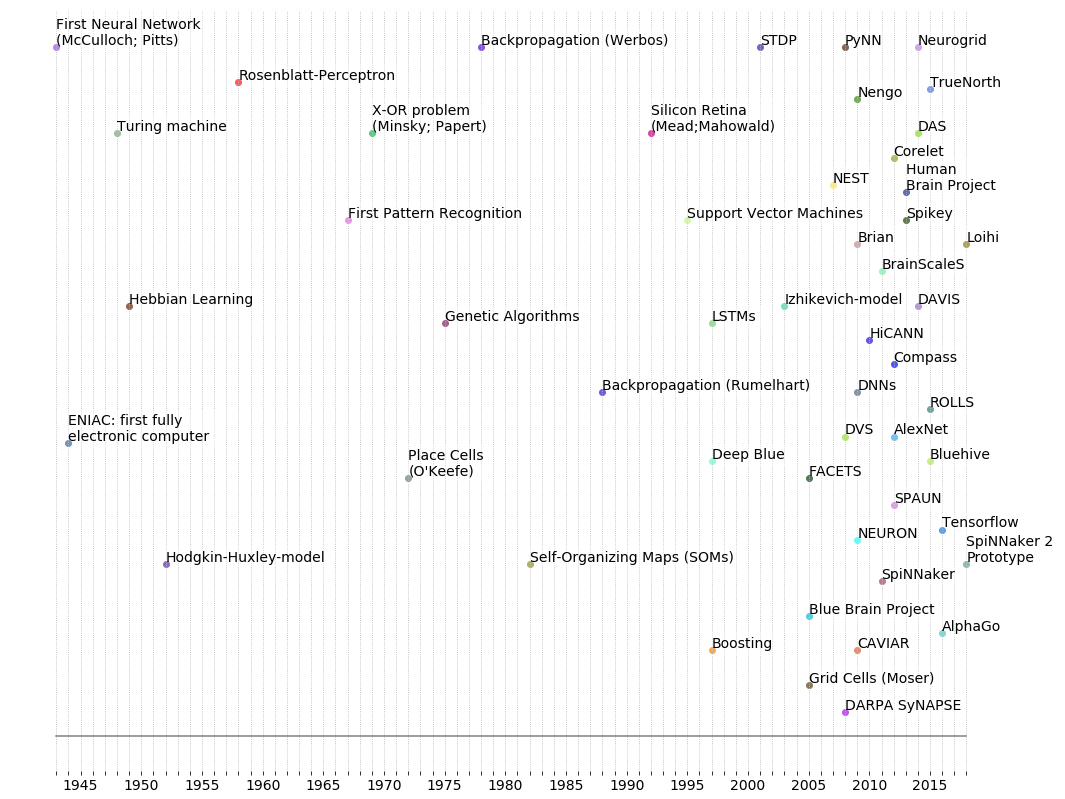
\includegraphics[width=0.95\textwidth,height=270px]{imgs/Neuromorphic_Timeline_beta.png}
	\caption{A selection of historical milestones in artificial intelligence, neuromorphic engineering and computational neuroscience. There is a significant boost of research and technologies in recent years.}
	\label{fig:neuro_time}
\end{figure*}
The research field of \aclp{ANN} goes back to the 1940s when McCulloch and Pitts introduced artificial neurons as computational units \cite{McCulloch1943}, which embody a simplified model of biological neurons.
These first simple networks were able to calculate compositions of basic logic functions \cite{McCulloch1943, Rojas1996}.
Rosenblatt \cite{Rosenblatt58} proposed the first neural network, which was capable of learning, by adding numerical weights to the connections of the network with threshold functions as activation functions: the \textit{perceptron}.
Minsky and Papert \cite{Minsky1969} showed, that single-layer perceptrons are not able to calculate an XOR-function or, more generally, are only capable of learning linearly separable patterns.
This caused a decreased interest in neural networks research until the rediscovery of the backpropagation algorithm \cite{Werbos1974} in the 1980s \cite{Rumelhart1986}, which introduced a practically feasible method to optimize the network weights using gradient descent and led to a resurgence of neural network research.
%This gradient descent called for continuous activation functions (mostly sigmoid or hyperbolic) instead of threshold-functions as activation functions, which made the so-called second generation \ac{ANN} universal approximators for continuous functions \cite{Cybenko1989}.
Since then, various different network architectures like feed-forward, \acp{CNN}, \acp{RNN}, \acp{RBF}, \acp{RBM}, \acp{SOM} and \ac{ART} just to name a few \cite{Schmidhuber2015} have been proposed for different learning paradigms.
Although several simpler methods like Boosting \cite{Freund1997} or \acp{SVM} \cite{Vapnik1995} have been developed and achieved noteworthy results, the availability of powerful, parallelized computing hardware like \acp{GPU} as well as the advent and success  of deep learning (partly achieving better-than-human accuracy) made \acp{ANN} \cite{Rojas1996} and especially \acp{DNN} \cite{LeCun2015} the state-of-the-art for several machine learning tasks like visual digit \cite{Ciresan2012a} and traffic sign \cite{Ciresan2012} recognition in recent years.
Another great achievement in the field of deep learning was the victory of AlphaGo \cite{Silver2016} over the world's best Go player Lee Sedol in March 2016, which was considered to be at least a decade away due to the complexity of Go.
Compared to Deep Blue, the system that beat former chess world champion Garri Kasparov in 1997 \cite{Hsu2002} with sheer computational power by brute forcing through a large number of possible moves in advance to find the best one, this strategy is not feasible for Go due to its higher complexity (larger board, more options to consider per move).
In contrast, modern \acp{DNN} trained by a combination of supervised learning from human expert games and reinforcement learning from self-play have been used for the evaluation of board positions and selection of moves to avoid expensive lookahead search \cite{Silver2016}.
A comprehensive and historical overview of relevant literature concerning \acp{ANN} and especially \acp{DNN} can be found in \cite{Schmidhuber2015, LeCun2015}.

\subsubsection{Neuromorphic systems}

The term neuromorphic itself was first introduced by Carver Mead in the late 1980s \cite{Mead90}, when describing one of the first silicon retinas.
He called artificial systems that share organization principles with biological nervous systems neuromorphic.
An interesting prototype of a silicon retina, which is now considered a milestone, was implemented by Misha Mahowald, a PhD student of Carver Mead.
Her thesis received Caltech's Milton and Francis Clauser Doctoral Prize for its originality and potential for opening up new avenues of human thought and endeavor.

Since these early days of neuromorphic engineering, the term has widely been used to describe \ac{VLSI} systems \cite{Mead1989}, novel computing devices \cite{Schemmel2010}, sensory systems \cite{Lichtsteiner2008, Liu2010}, software \cite{Davison2008, Bekolay2014} and algorithms \cite{ReverterValeiras2016}.
Considering the number of scientists, neuromorphic engineering is still a comparably young field of research but received an increased interest during the last decade from both academic and industrial research groups caused by the funding of large, ambitious projects.
Although there have been several achievements in the field during the 1990s \cite{Mead1989, Mahowald1992, Indiveri1997, Cauwenberghs1998} and early 2000s \cite{Liu2002}, the \ac{FACETS} project \cite{FACETS-proj} and the \ac{BBP} \cite{BlueBrain-proj}, both starting in 2005 and mainly funded by the \ac{EU} under the FP6-\ac{FET} program, were among the first big-budget neuromorphic projects.
The follow-up project \ac{BrainScaleS} \cite{BrainScaleS-proj, Schemmel2010} (2011-2015) built on and extended the research conducted during the \ac{FACETS} project.
The main developments of the \ac{FACETS} and \ac{BrainScaleS} projects are the \ac{HICANN} chip \cite{Schemmel2010} and the Python-based simulator-independent language \ac{PyNN} \cite{Davison2008} for building neural network models.
Building on \ac{BBP} the \ac{BrainScaleS} hardware development is currently continued in the neuromorphic computing platform of \ac{HBP} \cite{HBP-proj, Calimera2013}, a large ten-year research project, which was selected as one of the two \ac{EU}-\ac{FET} flagships in 2013 and is granted around one billion euros funding.
Another project starting in 2005, initially funded by the UK government until 2014 and now also part of the neuromorphic computing platform of \ac{HBP}, is the \ac{SpiNNaker} project \cite{Furber2014} during which the neuromorphic computing hardware of the same name was developed.
The \ac{HBP} is organized in thirteen platforms in total, which focus on different research fields related to the brain like for example theoretical neuroscience, neurorobotics, cognitive architectures, high performance computing, brain simulation and the aforementioned neuromorphic computing platform (see \cite{HBP-proj} for details).

Beside these research activities in Europe, the \ac{DARPA} funded another big-budget neuromorphic project: the \ac{SyNAPSE} program \cite{SYNAPSE-proj, Srinivasa2012}, which started in 2008 and is scheduled to run until 2016, has received 102.6 million US dollars in funding as of January 2013.
The program aims to build an electronic microprocessor system that matches a mammalian brain in function, size, and power consumption.
Achievements during the \ac{SyNAPSE} program, which is primarily contracted to IBM Research and \acs{HRL}, so far are include brain simulations, design of brain-inspired neuromorphic architectures \cite{Nere2012} and the development of a digital neurosynaptic core \cite{Merolla2011}, which is a building block of IBM's recently published TrueNorth chip \cite{Akopyan2015}.
Further project results are the Corelet language \cite{Amir2013} and the simulator Compass \cite{Preissl2012}, which enable dedicated software development as well as simulation and testing of TrueNorth algorithms on standard hardware respectively.

Beside these projects, the neuromorphic community is coming together at two annual  workshops in Telluride and CapoCaccia, which have been established in 1994 and 2007 respectively, to discuss the current state of research in lectures and interactive talk sessions, to forge new ideas and to work on hands-on projects in small work groups.

%----------------------------------------------------------------------------------------------------------
\subsection{\aclp{SNN}}
\label{subsec:SNN}
%----------------------------------------------------------------------------------------------------------
\begin{figure}[t!]
	\centering
	\resizebox{.9\textwidth}{!}{%
		\subfloat[\label{subfig:biological_neuron}]{%
			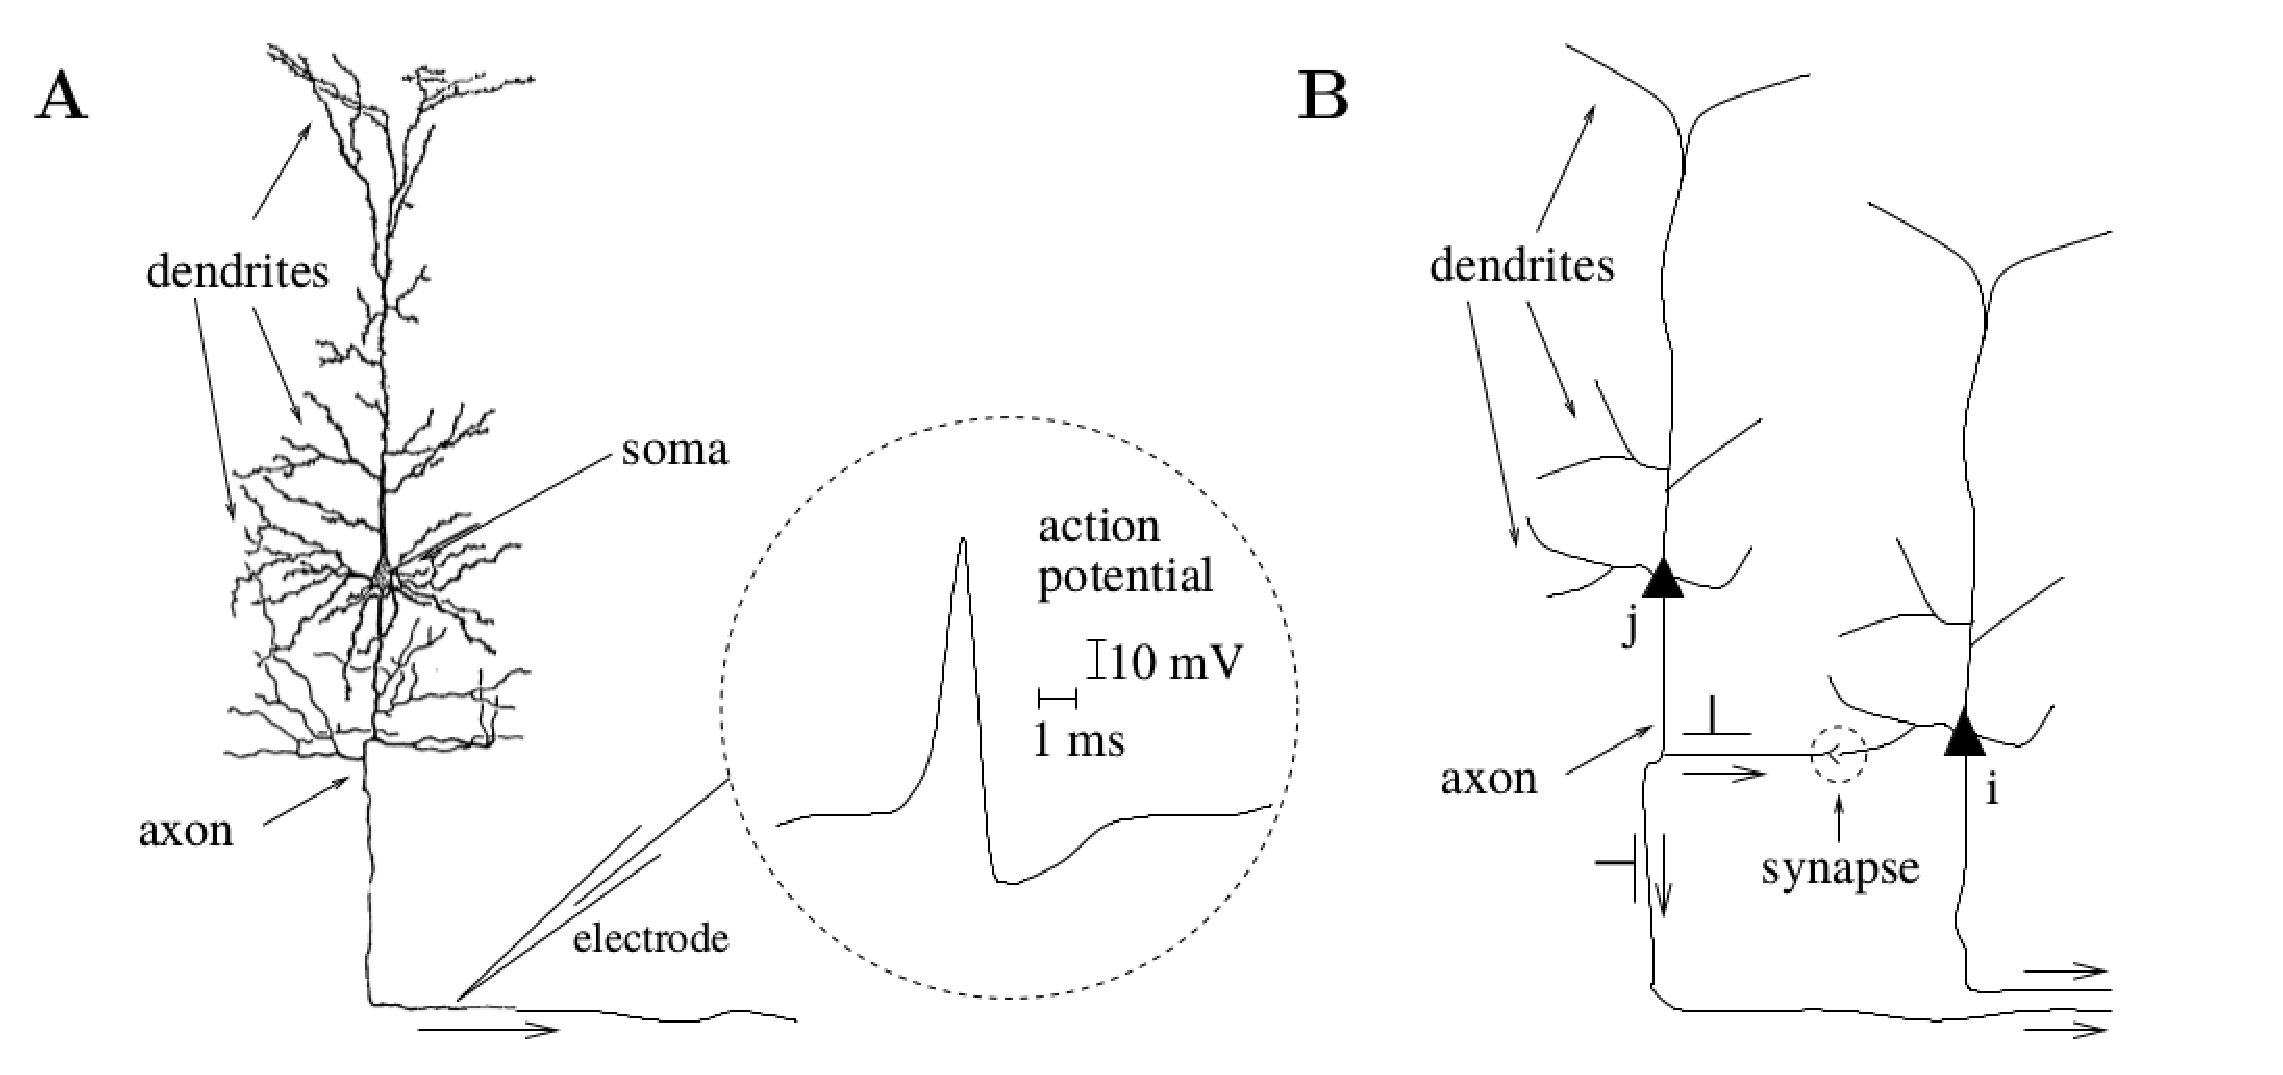
\includegraphics[height=3cm]{imgs/Neuron_model.eps}
		}
		\subfloat[\label{subfig:lif_neuron_model}]{%
			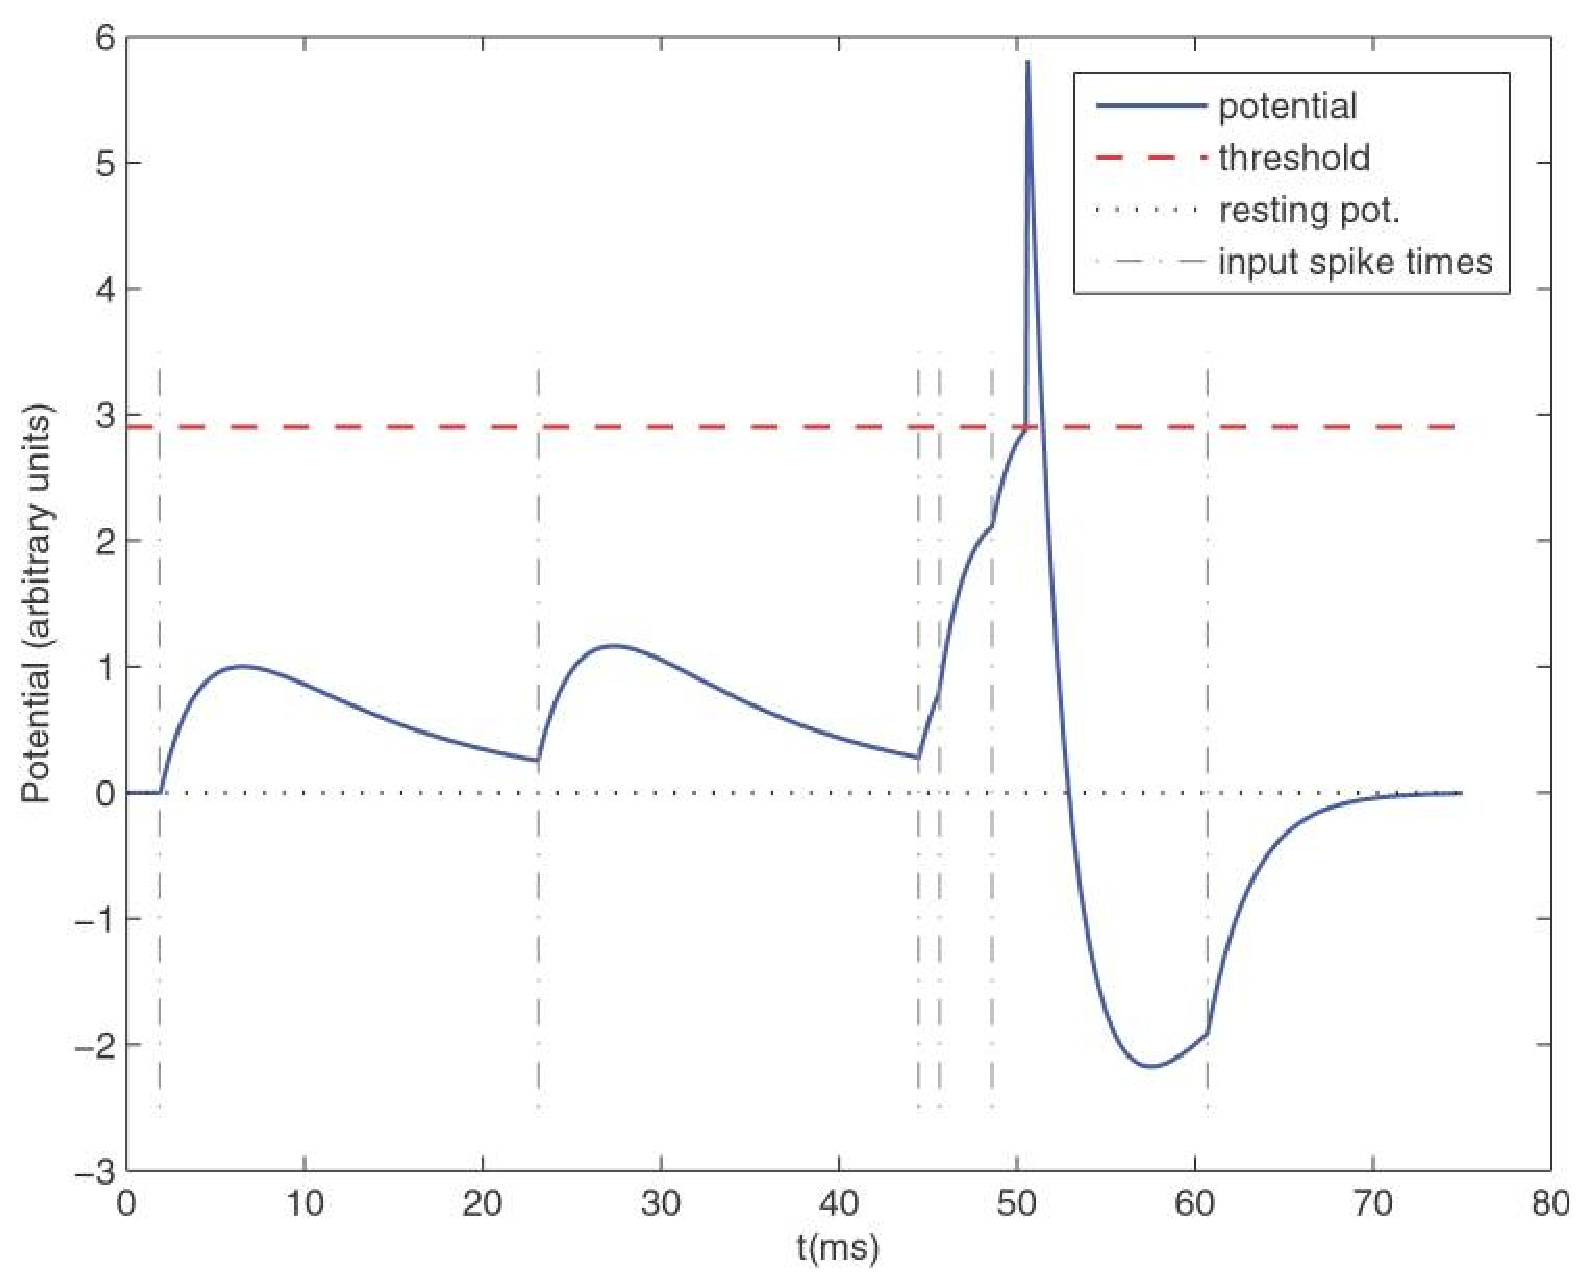
\includegraphics[height=3cm]{imgs/LIF_Neuron.eps}
		}
	}
    \caption{Visualization of different aspects of neuron models. ~\protect\subref{subfig:biological_neuron} depicts the structure and functioning of biological neurons in a schematic visualization (image source \cite{Gerstner2002}). ~\protect\subref{subfig:lif_neuron_model} visualizes the membrane potential's subthreshold behavior of a \ac{LIF} neuron model (image source \cite{Masquelier2007}).}\label{fig:neuron_models}
\end{figure}

Fig.~\ref{subfig:biological_neuron} depicts the structure and functioning principles of biological neurons.
They  exchange information by sending short and sudden pulses, so-called action potentials or spikes via synaptic connections.
Whenever the membrane potential of a neuron, which can be increased or decreased by incoming spikes depending on the synaptic weight, reaches a certain threshold, the neuron produces a spike itself and resets its membrane potential afterwards \cite{Gerstner2002, Paugam2009}.
Recent neuroscientific research suggests that the exact timing of those spikes encodes information rather than just average firing rates \cite{Bohte2004}.
While traditional \acp{ANN} used in machine learning neglect these biological details, \acp{SNN} embody these spike times and are therefore often referred to as the third generation of neural networks \cite{Maass1997, Paugam2009}.
Maass showed in \cite{Maass1997}, that \acp{SNN} have at least the same computational power as threshold and sigmoidal neural networks of similar size.

The simplest spiking neuron model is the \acf{LIF} model with
\begin{equation}
\frac{\partial V}{\partial t}(t) = - \frac{1}{\tau_{m}} \left( V\left(t\right) - R \cdot I\left(t\right) \right)
\label{eq:LIF}
\end{equation}
describing the subthreshold behavior of the neuron, where $V$ is the voltage across the membrane, $I(t)$ is the input current, $R$ is the passive membrane resistance and $\tau_{m}$ is the membrane time constant.
In other words, equation \ref{eq:LIF} states as follows: the membrane voltage increases in the presence of input current $I(t)$ depending on the membrane resistance $R$ while at the same time, especially in the absence of input current ($I(t)=0$), the voltage decreases or "leaks out" depending on the membrane time constant $\tau_{m}$.
When the voltage $V(t)$ passes a certain threshold $\vartheta$, the neuron produces a spike and the voltage is reset to a resting state $c$ for a certain refractory time interval $\tau_{ref}$ during which incoming spikes have no impact on the membrane potential.
Figure \ref{subfig:lif_neuron_model} visualizes the spiking behavior of the \ac{LIF} model.
It shows an example curve of the membrane potential of one \ac{LIF} neuron based on six incoming spikes whereas only the third, fourth and fifth incoming spike are appearing closely enough for the membrane potential to surpass it threshold and, therefore, cause the neuron to emit a spike itself.
The \ac{LIF} model, despite its biological simplifications, is maybe the most widely used neuron model for simulations due to its simplicity and comparably low computational complexity \cite{Izhikevich2004}, which allows simulations of large networks of neurons in reasonable time.
In contrast, the famous Hodgin-Huxley-model \cite{Hodgkin1952} with its four differential equations and dozens of (biologically meaningful) parameters is the model of high biological plausibility but also computationally challenging regarding large simulations \cite{Izhikevich2004}.
In 2003, Izhikevich proposed a neuron model \cite{Izhikevich2003} as compromise between biological plausibility and computational feasibility.
He showed that this simple model, described by two differential equations with four parameters, is able to produce all known spiking behaviors observed in cortical neurons \cite{Izhikevich2004}. 

One major hindrance for the widespread adoption of \acp{SNN} has been the problem, that standard learning algorithms for traditional \acp{ANN} like backpropagation \cite{Werbos1974} can not be directly applied to \acp{SNN}.
Although an analogon, the so-called SpikeProp algorithm \cite{Bohte2002} for \acp{SNN} has been developed, the more natural approach is to transfer and mimic biologically inspired learning approaches like Hebbian learning \cite{Hebb1949} or \ac{STDP} \cite{Bi2001}.
An overview of several learning approaches for \acp{SNN} possibly applied with neuromorphic hardware can be found in \cite{Walter2015}.
Another possibility is to train a traditional \ac{ANN} and convert the resulting network into a \ac{SNN} \cite{Diehl2015, Hunsberger2015}.
An example for this approach is the network performing the visual digit recognition task as part of the larger \ac{Spaun} model \cite{Eliasmith2012}, which was derived by training a \ac{DNN} consisting of four \ac{RBM} layers and converting this network using the principles of the \ac{NEF} \cite{Eliasmith2003}.
Although theoretically superior \cite{Maass1997}, \acp{SNN} have not yet outperformed state-of-the-art \acp{DNN} in terms of accuracy in practical machine learning applications \cite{Schmidhuber2015}.

Beside the aforementioned procedures to solve traditional machine learning tasks with \acp{SNN} and thereby encode artificial functions in spiking neurons, a different approach is to try to understand how complex cognitive behaviors and the underlying neural functions are performed in the brain.
Therefore, the question how the brain encodes complex information and behavior in trains of spikes and also how to decode these spike trains to reconstruct the encoded information needs to be answered.
Although modern research has shed some light on this question regarding the neural code, it is still mainly unanswered as we do not fully understand the anatomical and neurophysiological processes within the brain \cite{Stanley2013}.
Currently, there exist several approaches to code information as spike trains, which can be summarized by the categories rate coding, temporal coding \cite[Chap. 7.6]{Gerstner2014}, population coding \cite[Chap. 1]{Gerstner2002}, \cite{Ponulak2011, Boerlin2011} or sparse coding \cite{Olshausen1996}.
Except for the biologically unrealistic rate coding approach, there are cues for all of these coding schemes and even combinations \cite{Gupta2014} of them to appear in biological systems.

\subsubsection{Software tools}
There exist several different programming languages, simulators and software libraries specifically designed for modeling \acp{SNN} varying from tools like Corelet \cite{Amir2013} and Compass \cite{Preissl2012} working with one specific hardware component, in this case IBM's TrueNorth chip \cite{Akopyan2015} (cf. Sec. \ref{sec:neuromorphic_HW}), to libraries like \ac{PyNN} \cite{Davison2008}, which aim for universality to work with different simulators and hardware components as back-end.

The simulation tool offering maybe the highest level of abstraction is \ac{Nengo} \cite{Stewart2009}, which implements the principles of the \ac{NEF} \cite{Eliasmith2003} and was used to build the \ac{Spaun} model \cite{Eliasmith2012}.
Originally written in Java, \ac{Nengo} was re-implemented in Python \cite{Bekolay2014} and improved by incorporating the lessons learned from the creation of \ac{Spaun}.
\ac{Nengo} allows the user to describe a model on a high level of abstraction by defining groups of neurons to simulate different functional blocks while \ac{Nengo} takes care of neural properties and synaptic weights using the \ac{NEF} (see Sec. \ref{sec:neural_eng} for more details).
\ac{Nengo} models can be run using the internal simulation back-end, but also simulation on some neuromorphic hardware components like Neurogrid \cite{Dethier2011, Choudhary2012} and \ac{SpiNNaker} \cite{Mundy2015}, which are currently used in developments aiming to run the \ac{Spaun} model in real-time, is supported.

Another Python-based tool is \ac{PyNN} \cite{Davies2010}, which was developed during the \ac{FACETS} \cite{FACETS-proj} and \ac{BrainScaleS} \cite{BrainScaleS-proj} projects and aims for building \ac{SNN} models independent of actual simulation tools.
The level of abstraction is lower than \ac{Nengo}, but therefore it allows the creation of arbitrary neuron populations and connections, while the properties and synaptic weights need to be specified by the user or acquired using a learning algorithm.
\ac{PyNN} implements a number of standard models of neurons like \ac{LIF} or Izhikevich, connection algorithms like "one to one", "all to all" or connection matrices, static and plastic synapse types as well as several \ac{STDP} rules supported by the simulation and hardware back-ends.
Furthermore, \ac{PyNN} enables the user to implement custom models, connections and learning rules for advanced simulations and thereby extend the neural modeling toolkit.
\ac{PyNN} currently supports several different back-ends, e.g. simulators like \ac{NEST} \cite{Gewaltig2007}, Brian \cite{Goodman2009} and NEURON  \cite{Carnevale2009} as well as neuromorphic hardware.
\ac{PyNN} is currently the preferred development environment for the creation of \ac{SNN} models to run on the \ac{SpiNNaker} system \cite{Furber2014}.
The mapping of the network structure, neurons and synapses to actual cores on the chip is done with a separate software package called \ac{PACMAN} \cite{Galluppi2012}.

Another Python-based software package which, in contrast to \ac{PyNN} and \ac{Nengo}, mainly aims at modularity and flexibility in terms of supporting as many different neuromorphic hardware systems as possible as a front-end is \ac{PyNCS} \cite{Stefanini2014}.

A comprehensive overview of several other simulation tools for neural modeling can be found in \cite{Brette2007}.

%----------------------------------------------------------------------------------------------------------
\subsection{Neuromorphic Hardware}
\label{sec:neuromorphic_HW}
%----------------------------------------------------------------------------------------------------------

In this section, we give a brief overview of recent neuromorphic prototypes and hardware developments.
Although our work is not primarily targeted at use with this kind of dedicated hardware platforms, it shows promise regarding energy-efficiency and scalability in combination with specialized hardware components.
The neuromorphic prototypes described here are still comparatively young and not technologically mature yet, especially compared to traditional computing approaches.
Therefore, most of the hardware and sensors described are mainly developed and used in academia and are not standardized, commercial products yet.
However, this technology is gradually becoming available to a broader community and draws increased attention in industrial research groups.

\subsubsection{Digital Neurochips}
\acp{GPU} provide a \ac{SIMD} architecture which helps in parallel data processing at the expense of large power consumption \cite{Krichmar2011, Carlson2014}.
Due to fast matrix and vector multiplication capability of \acp{GPU}, at present they are providing an appealing platform for training and executing real-time data with the help of deep learning techniques \cite{Schmidhuber2015}.
For specific applications, which take several months of training on a traditional \acp{CPU}, \ac{GPU}-based systems can accomplish the tasks in days \cite{Edwards2015}.
A collaboration between NVIDIA and Stanford researchers demonstrated a cluster of \ac{GPU} servers which was able to train 1 billion parameters (scalable to 11 billion using 16 machines) on just 3 computers in two days.
Each machine contained 4 NVIDIA GTX680 \acp{GPU} with \SI{4}{\giga\byte} at \SI{1}{\tera\nothing}\ac{FLOPS} each.

One of the recent developments in digital neuro-chips is IBM's TrueNorth \cite{Akopyan2015}.
It contains a network of 4096 cores with 256 digital neurons each following a digital reconfigurable spiking neuron model \cite{Cassidy2013}, which makes over one million neurons and 256 million synapses in total consuming about \SI{65}{\milli\watt} of power.
The cores are connected internally by a 2-D grid.
The intersections of this grid contain routers which control the signal transmission within the network of cores inside a chip.
For programming this novel hardware implementation, a specialized programming language named Corelet was developed \cite{Amir2013}.

Another example of a digital neuromorphic hardware implementation is University of Manchester's \ac{SpiNNaker} Chip \cite{Furber2014}.
It contains 18 synchronously connected ARM968 microprocessors and \SI{128}{\mega\byte} \ac{DDR} \ac{SDRAM}.
Communication is carried out by a packet-switched on-chip network, where all chips have a router.
This architecture scales well to larger application by allowing to place more chips on a board \cite{Painkras2013,Navaridas2009}.
A \ac{SpiNNaker} system forms a toroidal mesh which has fixed connections, but the protocol implemented by the routers on the individual chips allows for the simulation of neural networks of arbitrary connectivity.

Another recent digital neuromorphic hardware platform is Intel's Loihi chip \cite{Davies2018}.
This chip consists of a fully asynchronous many-core mesh of $128$ neuromorphic cores, each containing $1024$ primitive units implementing spiking neuron behavior in a tree-like structure.
In total, it contains $130000$ artificial spiking neurons and $130$ million synapses.
One of Loihi's key features is the ability of on-chip learning, which is realized through a learning engine integrated in each core that enables the implementation of learning rules to adapt parameters of the core's \ac{SNN}.

\subsubsection{Analog Neurochips}

Most of analog chips do not allow on-chip training due to limited adaptability of implementation techniques like capacitors \cite{Schwartz1990}, floating gate transistors \cite{Holler1989}, \acp{CCD} \cite{Agranat1990}.
On the other hand, analog techniques use less components and offer high-speed operation.
To exploit the benefits of analog semiconductor technologies and neural adaptivity, the learning algorithms have to be implemented on-chip.
This, however, limits the reconfigurability of the platform and complicates the implementation of most learning rules directly into analog VLSI at the same time.
These limitations restrict the flexibility of analog designs compared to their digital counterparts.
%They possess similar functional properties as that of biological networks and can be interfaced directly with real analog world \cite{Mead90}.

The \ac{HICANN} chip \cite{Schemmel2008} has the capability to simulate $131072$ synapses and $512$ neurons residing inside an \ac{ANC}.
For simulation of large networks a wafer-scale integration method was used, which enabled $384$ \ac{HICANN} chips to be interconnected on a wafer of \SI{20}{\centi\meter} diameter \cite{Schemmel2010}.
The spikes between various \acp{ANC} on a wafer or between interconnected wafers are carried out by a network of horizontal and vertical grid like structure.
The horizontal pathway consists of 64 bus lines which carry spikes from 64 neurons.
The 256 vertical lines collect spikes for all connected \acp{ANC}.
The spikes are represented as data packet of 6-bits (for the group of 64-neurons) and transmitted using \ac{AER}. 

The \ac{ROLLS} consists of $256$ neurons and $131072$ synapses.
It consumes only \SI{4}{\milli\watt} of power and uses exponential \ac{IF} modeling \cite{Qiao2015}.
The latest processor contains different configuration options.
Each neural circuit is connected to three different types of synaptic circuits, first of which is an array of $256\times256$ synapse which can be excitatory or inhibitory.
The synapses in the second $256\times256$ array offers only excitatory mode.
In the third array, there are $256\times2$ virtual synapses whose weights are configurable with excitatory as well as inhibitory features. The virtual synapses operate in shared mode and occupy less space as compared to individual circuits.
The neural spikes are generated and received using an \ac{AER} protocol with 8-bit neuron addresses \cite{Qiao2015}.

Another example of analog neural hardware is a chip \cite{Srinivasa2012} developed under \ac{DARPA}-funded \ac{HRL} \ac{SyNAPSE} project, which uses \ac{STM} for computation and memristors for synaptic weights storage.
It contains a total of 576 neurons and 73728 synapses, arranged in an array of $24\times24$ neurons each with $128$ synapses and consumes \SI{130}{\milli\watt}.
In \ac{STM} methodology a single synaptic circuit on the chip calculates multiple logical synapses of the simulated neural network because the electrical circuitry can function at much higher speeds than biological neurons.
Hence a single synaptic circuit can emulate multiple logical synapses by switching between the corresponding parameter sets.
There is a point-to-point routing mechanism hence no \ac{AER} is required \cite{Walter2015}. 

The Brain in Silicon group at Standford University developed the custom board Neurogrid, which contains 16-Neurocores \cite{Benjamin2014, Choudhary2012}.
The neuron circuits are arranged in a 256$\times$256 grid, with every neuron has separate circuits for its soma and the dendrite.
They combined analog computations with digital communication.
The system is capable of simulating one million neuron and eight billion synapses in real-time and consumed \SI{3.1}{\watt} of power.
The spikes are transmitted using \ac{AER}.
It additionally implements a deadlock-free wormhole routing protocol to ensure free transmission of packets.
It offers to explore different cortical areas of the brain by programming each of the Neurocores with a different model \cite{Merolla2014}.

\subsubsection{Neuromorphic Sensors}
\label{subsubsec:neuro_sensors}
\begin{figure}[t!]
	\centering
	\subfloat[]{\label{subfig:DVS_rotationg_dot}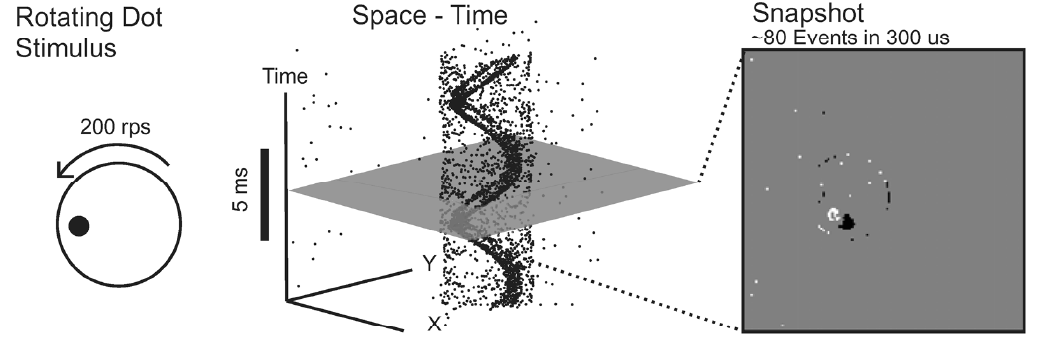
\includegraphics[width=0.9\textwidth]{imgs/DVS_rotating_dot_stimulus.PNG}}
	\par\medskip
	\begin{minipage}{.48\columnwidth}
		\centering
		\subfloat[]{\label{subfig:DVS_pixel_core}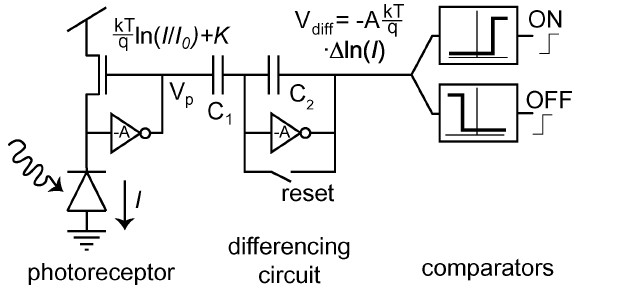
\includegraphics[width=1.15\textwidth]{imgs/DVS_pixel_core.PNG}}
	\end{minipage}%
	\begin{minipage}{.48\columnwidth}
		\centering
		\subfloat[]{\label{subfig:DVS_operation_principle}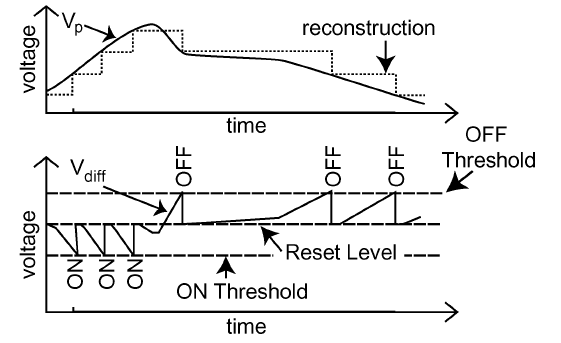
\includegraphics[width=0.9\textwidth]{imgs/DVS_operation_principle.PNG}}
	\end{minipage}\par\medskip
	\caption{(a) Space-time representation of the event stream generated by a rotating dot on a spinning disk and a snapshot of the events (b) abstracted pixel core schematic (c) principle operation of single DVS pixel. Image source: \cite{Lichtsteiner2008}}
	\label{fig:DVS_with_schem}
\end{figure}
To adopt the neuromorphic hardware in real-world applications (e.g. neurorobotics), they need to be able to process sensors signals.
The neurally inspired, non von-Neumannian architecture requires either a new generation of sensors, e.g.\ the \ac{DVS} \cite{Lichtsteiner2008}, \ac{DAVIS} \cite{Brandli2014} or \ac{DAS} \cite{Liu2014}, which already embody the spiking neuron signal processing or a way of translating traditional sensor signals to sequences of spikes.
Several approaches to encode signals and stimuli with trains of spikes, e.g. by rate coding, temporal coding \cite[Chap. 7.6]{Gerstner2014} or population coding \cite[Chap. 1]{Gerstner2002}, \cite{Ponulak2011} have been investigated.
Neuromorphic sensors on the other hand, directly emit a sequence of events without the need of translation.
The \ac{DVS} for example, unlike traditional frame-based cameras, generates spike events \cite{Lichtsteiner2008} asynchronously for individual pixels when perceiving relative illumination changes (see Fig. \ref{fig:DVS_with_schem}), which are key features of biological vision \cite{Lichtsteiner2008}.
This event-based approach offers several advantages compared to conventional frame-based cameras like the ability to perceive very fast movements (sub-millisecond time precision) without the need to wait for and process the next frame as well as an output data rate depending on the dynamic content of the scene (Fig. \ref{subfig:DVS_rotationg_dot}) and thus reducing the output of redundant information.

The \ac{DVS}-pixels were designed to cover wide dynamic range and to offer low latency and mismatch.
This is achieved by a fast photoreceptor circuit with logarithmic response whose output is fed into a high precision difference amplifier circuit followed by a two-transistor comparator circuit (see Fig. \ref{subfig:DVS_pixel_core} and \ref{subfig:DVS_operation_principle}).
%The pixels are arranged in rows and columns which have $x$, $y$-address.
The comparator circuit produces ON and OFF signals for each pixel, which are passed to the \ac{AER} interface for transmission via USB2.0 interface. \cite{Lichtsteiner2008}.
On the other hand, the \ac{DAVIS} employs an \ac{APS} circuit to output synchronous global shutter frames, which helps in persevering absolute intensity information needed for classification and object recognition tasks while asynchronous \ac{DVS} events are beneficial for the tracking of fast movable objects \cite{Brandli2014}.


\subsection{Neuromorphic Applications}
\label{subsec:neuro_applic}

In this section we present some examples of applications of neuromorphic hardware and sensors described in Sec. \ref{sec:neuromorphic_HW}, software, algorithms and neural modeling depicted in Sec. \ref{subsec:SNN} as well as combinations of both.
First, we describe applications using either neuromorphic sensors or hardware in combination with traditional computing hardware.
Then, we focus on purely neuromorphic systems, where the spiking signals of neuromorphic sensors, mainly the \ac{DVS}, is processed by neuromorphic hardware.
Although there are currently - to the knowledge of the author - no neuromorphic actuators working directly on the basis of spikes, we refer to the robotic systems described here as purely neuromorphic.


\subsubsection{Mixed systems}
\label{subsubsec:mixed_sys}

Neuromorphic vision \cite{Tan2015} is an emerging field of research, which aims to transfer approaches from traditional computer vision and also establish new methods incorporating the characteristics of the \ac{DVS}.
To perform pattern recognition tasks with neuromorphic cameras and at the same time use traditional methods as a benchmark, existing image data bases like the \ac{MNIST} data set \cite{LeCun1998} are translated to neuromorphic data sets by presenting the images on a computer screen to a \ac{DVS} sensor moving minimally back and forth \cite{Orchard2015} (mimicing saccade movements of the human eye), which gives better results than moving the images themselves on the screen \cite{Serrano-Gotarredona2013}.

As the \ac{DVS} naturally captures moving objects when held statically and cues of the ego-motion when moving, tracking of these movements are suitable applications making use of the sensor's characteristics.
These characteristics along with the \ac{DVS}'s advantages compared to traditional frame-based cameras, which have been described in Sec. \ref{subsubsec:neuro_sensors}, have been demonstrated in applications like pencil balancing \cite{Conradt2009} and a robotic goalie \cite{Delbruck2013} interfacing the \ac{DVS} with traditional computing hardware and actuators.
Keeping track of (geometric) features \cite{Lagorce2015} and contours \cite{Barranco2014} observed by the \ac{DVS} lays the foundation for more sophisticated algorithms.
Researchers recently proposed several approaches for tracking people \cite{Schraml2010, Piatkowska2012} and other geometric objects \cite{ReverterValeiras2016} using stationary sensors.
Especially tracking at high velocities \cite{Saner2014} benefits largely from the sub-millisecond time precision of the \ac{DVS} even enabling tracking of particles in fluid flows \cite{Drazen2011}, which would require a high-speed PC, lots of disk space and high-intensity laser strobe lighting to illuminate the fluid in a conventional setting.

A traditional application of computer vision in robotics is the estimation of the ego-motion or odometry based on optical flow (an event-based approach on optical flow can be found in \cite{Benosman2014}), which can also be obtained by combining traditional cameras with the \ac{DVS} on a small wheeled robot \cite{Censi2014}.
Another suitable application for the \ac{DVS} is the estimation and tracking of the whole six degree-of-freedom pose of a flying robot, especially when performing high-speed maneuvers, where traditional cameras suffer from motion blur \cite{Mueggler2014}.
Another problem in robotics closely related to tracking is self-localization of the robot using a given map of the environment or building a map online and localizing within this map at the same time, which is known as the \ac{SLAM} problem \cite{Thrun2005}.
Localization performed within a given map using the \ac{DVS} on ground vehicles and by tracking markers from a flying robot is presented in \cite{Gallego2015} and \cite{Censi2013} respectively.
There are also several papers treating the \ac{SLAM} problem \cite{Weikersdorfer2012, Weikersdorfer2014} or the related problem of tracking the camera pose and simultaneously reconstructing the observed scene by mosaicing \cite{Kim2014} with neuromorphic vision sensors.

Most of the tracking algorithms mentioned here use variations of traditional Bayesian filters like (extended) Kalman- or particle-filters \cite{Thrun2005} for consecutive estimation of the quantity of interest.
However, due to the asynchronous information processing of the \ac{DVS} or neuromorphic systems in general these filters need some modifications to work with this event-based approach \cite{Weikersdorfer2013} like taking several past measurements into account (in contrast to the traditional Markov assumption) or updating only after a certain number of events have occurred to avoid computational overhead.

In \cite{Axenie2015}, the authors describe a biologically inspired system for sensor-fusion of several traditional sensors like wheel encoders, magnetometer and gyroscope for ego-motion estimation demonstrated in ground and flying robots.
Another example for sensor fusion is presented in \cite{OConnor2013}, where the biologically inspired \ac{DVS} and \ac{DAS} sensors are used to recognize hand-written digits from the \ac{MNIST} data set \cite{LeCun1998}.
To incorporate the neuromorphic audio sensor, each digit is assigned one tone frequency in the A harmonic minor scale, while the actual fusion is performed by a \ac{DBN} consisting of several, pre-trained (unsupervised) \ac{RBM} layers, which was traditionally trained and afterwards transferred to an event-based network.
Although the authors state that the actual implementation in \cite{OConnor2013} is just a proof-of-concept in software, their approach shows promise to translate fully trained \acp{DBN} to \acp{SNN}, deploy them on efficient neuromorphic chips and thereby making this technology available for mobile and/or real-time applications.

To demonstrate the functionality and applicability of their neuromorphic chip TrueNorth, IBM implemented several proof-of-concept applications ranging from virtual robots, game simulations \cite{Arthur2012}, digit recognition \cite{Arthur2012, Esser2013} to classical machine learning tasks like object detection \cite{Akopyan2015}.
In \cite{Arthur2012} the authors present four example applications of neural algorithms implemented on TrueNorth using the Corelet language: a virtual robot driver aiming to keep the simulated robot on a virtual road based on visual cues, a neural algorithm controlling an autonomous player performing the classical video game pong, a neural implementation recognizing hand-written digits of the \ac{MNIST} data-base using \acp{RBM} as well as a Hopfield network, which performs autoassociation.
Seven example algorithms and applications for TrueNorth are presented in \cite{Esser2013}: speaker recognition using \acp{CNN} on the \ac{CUAVE} data set \cite{Patterson2002}, composer recognition distinguishing between classical composers Bach and Beethoven using liquid state machines, recognition of hand-written digits of the \ac{MNIST} data set using population coding and \acp{RBM}, a neural implementation of a \ac{HMM}, collision avoidance using motion extraction and looming detection, optical flow based on \acp{CNN} and eye detection using the \ac{DVS}.
Most of these algorithms are simplified proof-of-concept implementations showing the general applicability of TrueNorth but are not competitive with traditional machine learning algorithms yet (e.g. \SI{92.34}{\percent} \cite{Esser2013} vs. \SI{99.77}{\percent} \cite{Ciresan2012a} correct classifications on \ac{MNIST}).
In \cite{Schmitt2017}, the authors demonstrate training and deployment of \acp{DNN} on the \ac{MNIST}-data set using the \ac{BrainScaleS} hardware.
A more sophisticated application is the multi object detection and classification task described in \cite{Akopyan2015}, which detects moving and stationary people, bicyclists, cars, buses and trucks from a HD video stream in real-time recorded by a stationary camera using Haar-like features, saccades, K-means- and Grid-classifiers.

The use of the neuromorphic hardware Neurogrid \cite{Benjamin2014} as computational back-end for \ac{Nengo} and proof-of-concept solution for medical motor-prostheses, which shall be connected to biological neurons and thereby be controlled by the patient's brain, is described in \cite{Choudhary2012} and \cite{Dethier2011} respectively.
The \ac{SpiNNaker} system \cite{Furber2014} also supports the simulation of neural models created using \ac{PyNN} or \ac{Nengo} \cite{Mundy2015}.
Furthermore, several neural network architectures like \acp{CNN} \cite{Serrano-Gotarredona2015} and pre-trained \acp{DBN} \cite{Stromatias2015, Stromatias2015a} have also been implemented on the \ac{SpiNNaker} system.

To enable biologically inspired learning like \ac{STDP} \cite{Bi2001}, according rules adapting the synaptic weights depending on the timing of the spikes have efficiently been implemented on the \ac{SpiNNaker} \cite{Diehl2014} chip as well.
\todo{include phrase about own omnibot paper \cite{Mirus2018a}}
\subsubsection{Purely neuromorphic systems}
\label{subsubsec:neuro_systems}

\begin{figure}[t!]
	\centering
	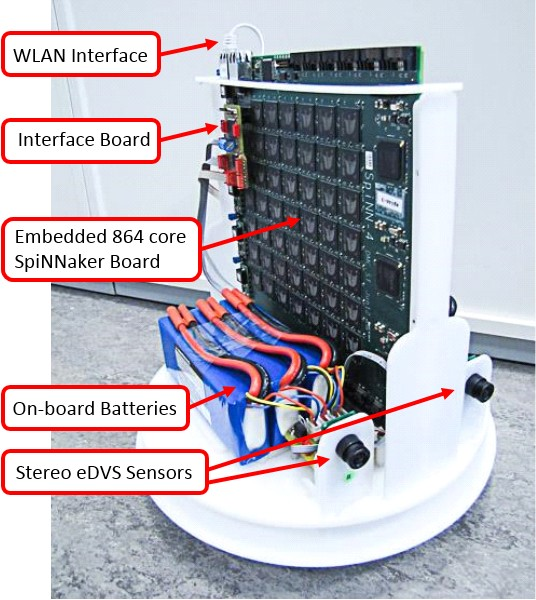
\includegraphics[width=0.48\textwidth]{imgs/SpinRobot.jpg}
	\caption{Example of a closed-loop, neuromorphic robotic system with two event-based embedded \acp{DVS} and a 48-node \ac{SpiNNaker} board. Image source: \cite{Galluppi2014}}
	\label{fig:spin_robot}
\end{figure}
Some examples of closed-loop systems deployed in small robots are presented in \cite{Davies2010, Denk2013, Galluppi2014}.
In \cite{Davies2010, Denk2013}, the authors interface two embedded \ac{DVS} cameras directly with a \ac{SpiNNaker} platform mounted on a small robot (see Fig. \ref{fig:spin_robot}).
The implemented neural networks enable simple autonomous behaviors like following a line \cite{Davies2010} or approaching a light stimulus \cite{Denk2013}.
In \cite{Galluppi2014}, a small robot with a similar setup is able to perform trajectory stabilization using optical flow from the \ac{DVS} cameras as input.
Another simple task described in \cite{Galluppi2014} is the recognition and tracking of a light stimulus and keeping the robot at a certain distance and angular orientation with regard to this stimulus.
The whole processing chain from visual perception over internal processing to motor control in these robot experiments are realized using spiking neuron models.
The neural implementation of the latter two applications are done in \ac{PyNN} and \ac{Nengo} respectively.

While the aforementioned sensorimotor behaviors are manually engineered, there are attempts to learn more sophisticated, complex behaviors from simpler basic movements \cite{Conradt2014, Stewart2016}.
These basic maneuvers are still manually engineered relating sensor cues to simple movements like driving forward with no obstacle in the sensors field of view, turning with an obstacle in in front of the robot or driving backwards when being close to an obstacle.
In \cite{Conradt2014} the authors describe a method on learning more sophisticated behaviors from recorded sensorimotor data obtained from driving the robot by remote control as training examples, which can be considered as a supervised learning approach.
In \cite{Stewart2016}, the training examples are taken from recording data of the robot driving around without human interference and just labeling those situations as positive examples when the robot performed the desired action by accident, which is considered as reinforcement learning.
Both approaches are implemented on a small robot with the \ac{DVS} as sensory input using \ac{Nengo} and the \ac{NEF} as well as its interface \cite{Mundy2015} for running neural networks models on the \ac{SpiNNaker} hardware \cite{Furber2014}.
% %----------------------------------------------------------------------------------------------------------
% \section{\aclp{ANN}}
% \label{sec:ML_ANN}
% %----------------------------------------------------------------------------------------------------------
% Machine learning in general is the science of constructing computer programs, which improve with experience.
% This is attractive if manually programming a desired functionality is not cost-efficient, intractable or simply impossible.
% The overall goal of machine learning algorithms is to generalize beyond examples, i.e. to generate models that describe the presented input sufficiently well to make the best possible prediction when confronted with previously unseen data.
% A formal, widely cited definition of machine learning has been presented by Thomas M. Mitchell in \cite{Mitchell1997}:
% \begin{defn}
% 	A computer program is said to \textbf{learn} from experience $E$ with respect to some class of tasks $T$ and performance measure $P$ if its performance at tasks in $T$, as measured by $P$, improves with experience $E$.
% \end{defn}
% A large body of research has focused on machine learning during the last decades.
% One major branch of machine learning are \acp{ANN} and \acp{DNN} in particular, which are currently the state-of-the-art of many machine learning tasks.
% \subsection{A brief history}
% \subsection{Supervised Learning}
% \todo[inline]{brief introduction to \acp{DNN} in general, particularly \acp{CNN} for classification, mentioning automotive related applications. Also mention \acp{RNN} and especially \ac{LSTM} as for time-series analysis/prediction as it is related to our behaviour prediction task}
% \subsection{Unsupervised Learning}
% \todo[inline]{brief introduction some unsupervised learning strategies. Focus especially on approaches to learn word embeddings like word2vec \cite{Mikolov2013}, GloVe \cite{Pennington2014}. Also mention problems of those approaches \cite{Levy2015}}
% \subsection{Reinforcement Learning}
% \todo[inline]{very brief introduction. Not sure yet if we need this secton at all}
%From the first theoretical considerations concerning artificial neural networks by McCulloc and Pitts(\todo{Citation}) in the 1940s and the first Multilayer-Perceptrons by Rosenblatt (\todo{Citation}) about a decade later, machine learning algorithms started to receive widespread attention with the rediscovery \cite{Rumelhart1988} of the well-known backpropagation algorithm \cite{Werbos1974}.
%Since then, several approaches to machine learning, apart from artificial neural networks, like AdaBoost (\todo{Citation}), Decision Trees (\todo{citation}), Bayesian Networks (\todo{citation}) or \ac{SVM} (\todo{citation Vapnik, V. (1995), The Nature of Statistical Learning Theory. Springer Verlag, Cristianini, N. and Shawe-Taylor, J. (2000). An Introduction to Support Vector Machines and Other Kernel-Based Learning Methods. Cambridge University Press, Cambridge}) have been proposed.
%These methods vary in representation of the data, the evaluation (or objective) function, the optimization technique and the learning paradigm.
%Through availability of larger datasets and increased computational power, machine learning has seen significant progress in recent years.
%The use of deep neural networks \cite{Schmidhuber2015}, enabled through modern, powerful computing hardware like \ac{GPU}, yielded a significant performance boost in several classification tasks.
%Today, modern deep learning algorithms can even rival human performance on different visual classification tasks like traffic sign \cite{Ciresan2012} or digit recognition \cite{Ciresan2012a}.
%
%So-called second generation \ac{ANN} introduced continuous (e.g. sigmoid or hyperbolic) instead of step- or threshold-functions (\todo{Citation}) as activation functions, which made them universal approximators for continuous functions \cite{Cybenko1989}.
%The term "neuromorphic" was first introduced by Carver Mead in \cite{Mead90}, when describing one of the first silicon retinas.
%For clarity, a first broad definition is provided, which will need some refinement while proceeding in this section:
%\begin{defn}
%\label{def:neuromorph}
%Artificial systems, that share organization principles with biological nervous systems are called \textbf{neuromorphic}.
%\end{defn}
%Biologically inspired systems and algorithms have seen significant progress and achieved remarkable results, e.g. in the field of machine learning, despite some simplifications in terms of biological accuracy.
%So-called first and second generation \ac{ANN} described in \ref{subsec:ML_ANN} are also covered by definition \ref{def:neuromorph} as neuromorphic systems, although they neglect some biological details.
%\subsection{Spiking Neural Networks}
%Biological neurons exchange information by sending short and sudden increases in their membrane voltage, so-called action potentials or spikes.
%Recent neurological research suggests that the exact timing of those spikes encodes information rather than just average firing rates (\todo{Citation}).
%While \ac{ANN} of the first two generations neglect these biological details, recent neural networks structures, so-called \ac{SNN} \cite{Paugam2009}, embody these spike times and are therefor often referred to as the third generation of neural networks .

\section{Cognitive Modeling}%
\label{sec:cognitive_modeling}

Over the last decades, understanding and building cognitive systems has seen extensive research leading to the development of several cognitive architectures.
A cognitive architecture is a "general proposal about the representation and processes that produce intelligent thought" \cite{Thagard2012}.
On the one hand, these architectures are used to explain and better understand important aspects of human behavior and intelligence.
However, they are also used to design computers and robots mimicking certain cognitive abilities of humans.
In this respect, cognitive architectures are typically clustered in three main categories, namely symbolism, connectionism and dynamicism \cite{Eliasmith2013}.
We will give a brief overview over symbolic and connectionist approaches in subsequent sections, whereas dynamicism \cite{Schoener2008} is of lower relevance to the work at hand.

One important aspect of cognitive modeling and, more generally, \ac{AI}, is knowledge representation.
Any intelligent agent, artificial or biological, that wants to perform reasoning about the world it encounters, needs to be able to build an internal representation of its perceived information.
This aspect is quite important for subsequent chapters, while a formal definition of what knowledge representation actually is appears to be difficult and thus is often avoided in the literature \cite{Davis1993}.
In \cite{Davis1993}, the authors describe five defining roles, that such a representation can play.
A representation is a surrogate, i.e., an internal substitute for a real-world entity and as such an imperfect approximation.
Therefore, the choice for each representation implies a set of ontological commitments, which effect the focus of attention of the representation.  
When the focus of such a representation is to enable some kind of reasoning in intelligent machines or robotic systems, these systems need to be able to manipulate the representation and perform computations with it.
Finally, as long as the machine needs to interact or communicate with humans in the sense that humans inform the machine about the world by e.g.\ creating a representation, this representation itself also plays the role of a medium of human expression.

\subsection{Symbolic approaches}%
\label{subsec:symbolic_approaches}

Symbolic approaches are often referred to as the "classical approach" to cognitive modeling or \acf{GOFAI}.
Most of the approaches rely on the metaphor of the "mind as computer", supposing that cognitive systems have a symbolic "language of thought" \cite{Fodor1975}, that expresses the rationale and rules the systems follow.
The corresponding analogue for computers are programming languages.
The dominant paradigm of such approaches is "the manipulation of discrete atomic symbols by explicit rules" \cite{Levy2008}.
The most prominent approaches in this category are production systems, which typically rely on if-then-rules (or productions) and a control structure.
One of the first and most influential achievements in this field is a program called the \ac{CogGPS}, which was able to to solve elementary problems in symbolic logic on its own.
The steps \ac{CogGPS} performed to solve a given problem often matched the steps reported by people solving the same problem.
This success enabled the development of several other cognitive architectures such as Soar \cite{Laird1987}, \ac{EPIC} \cite{Kieras1997} and \ac{ACT} \cite{Anderson1983} and its successor \ac{ACT-R} \cite{Anderson1996}, which all employed production systems at their core but adding their own extensions.
\ac{ACT-R} is the most modern of these architectures and arguably the most successful and thus most widely used cognitive architecture.
Although \ac{ACT-R} incorporates some connectionist-like mechanism in its memory system, it is widely considered a symbolic architectures as it relies on symbolic representations and a production system as central procedural core.
In general, symbolic approaches to cognitive modeling had the most success when addressing higher-level cognitive tasks, with a rigid set of rules and potential for pre-specified solutions.
However, these approaches are rarely used when it comes to real-time critic systems such as robots or if the system needs to generalize beyond pre-specified situations.

\subsection{Connectionist approaches}%
\label{subsec:connectionist_approaches}

One of the first theories challenging the paradigm of \ac{GOFAI} was the "Society of Mind" \cite{Minsky1986} view of specialized individual agents cooperating to accomplish a certain goal.
The strongest challenge however, was the emergence of connectionism \cite{Rumelhart1986a} (popularly referred to as neural networks), which offered novel learning algorithms such as backpropagation \cite{Rumelhart1986} to solve a wide variety of problems.
Connectionism explains cognitive phenomena by constructing models consisting of large networks of interconnected nodes performing rather simple input/output mappings.
If these nodes, however, are connected to sufficiently large networks, the nodes' activity is able to implement cognitive behavior such as rules or analyzing patterns.
We already gave a brief historical overview over the research conducted related to \acp{ANN} in section ~\ref{subsec:history_neural_nets}. 
The metaphor behind connectionist approaches to cognitive modeling is that of the "mind as brain", as the processing employed in connectionism is often referred to as "brain-like" or "brain-inspired".
Connectionism has shown remarkable results in diverse applications such as computer vision, pattern recognition, sequential data analysis and language processing just to name a few.
However, the most serious criticism of connectionist approaches are that they could not exploit systematic, compositional representations or logical reasoning of the form used in \ac{GOFAI}. 
Furthermore, the nodes in connectionist networks typically simplify the computational and representational properties of biological neurons, which in addition to the biological implausibility of the backpropagation algorithm, concerns cognitive modelers interested in biological realism.
Finally, the ability to learn and derive internal representations of features from data, despite being one of the greatest strengths of neural networks approaches, is sometimes criticized for lack of comprehensibility.

\subsection{Vector-based approaches}%
\label{subsec:vector_based_approaches}

To address some of the concerns regarding both, symbolic and connectionist approaches to cognitive modeling, researchers developed a hybrid approach often referred to as \acf{VSA}, a class of connectionist distributed representations.
In chapter ~\ref{chap:introduction_to_vsas}, we give an in-depth introduction to the theory and mathematical properties of \acp{VSA}, which will be import ingredients for the remainder of the thesis.
Here, we give a brief overview of the different variants of such architectures, their similarities and differences, related work and some applications.
All of the modeling approaches presented in this section employ (high-dimensional) vectors as representational units.
Similar to the representations derived from connectionist approaches, these are distributed representations, which offer nice properties such as robustness to noise and the support of distance metrics.
Additionally, all of the approaches allow to treat such vectors as "symbol-like" entities, which can be manipulated through the architecture's algebraic operations (see chapter ~\ref{chap:introduction_to_vsas} for details).
The first attempt on structured vector representations used the tensor product as multiplication operation \cite{Smolensky1990} to bind two different vector together.
The tensor product approach already allows for an sufficiently complex embedded structure to do linguistic processing.
However, scaling becomes a problematic issues as each uncompressed tensor product operation of two high-dimensional vectors increases the result's dimension, which quickly becomes impracticable.
Hence, there are several architectures such as \ac{MAP} \cite{Gayler1998, Gayler2003}, \acp{BSC} \cite{Kanerva1988} and \acp{HRR} \cite{Plate1991, Plate1994}, which propose different compressed multiplication operations replacing the tensor product and resulting in vectors with the same dimension as the input vectors.
Furthermore, these different \ac{VSA} variants differ in the choice of the numerical space to pick the vectors' elements from, i.e., if they use binary, real- or complex-valued vectors. 
The \ac{SPA} \cite{Eliasmith2013} is built upon \acp{HRR} and extends these architectures, by proposing an efficient mechanism of implementing structured vector representations in populations of spiking neurons using the principles of the \ac{NEF} \cite{Eliasmith2003} (again, we refer to chapter ~\ref{chap:introduction_to_vsas} and especially sections ~\ref{sec:neural_eng} and ~\ref{subsec:implementation_in_snns} for further details).   

The most prominent application of vector representations despite cognitive modeling \cite{Blouw2016, Crawford2016, Eliasmith2012} is language processing \cite{Gayler2003}.
In this context, word embedding refers to the problem of finding (or automatically learning) desirably meaningful representations for words.
Modern word embedding algorithms such as word2vec \cite{Mikolov2013, Mikolov2013b} or \ac{GloVe} \cite{Pennington2014} employ high-dimensional vectors as representational structure to encode words and language by learning in unsupervised fashion from large corpora of text.
There are also attempts of using such representations in other domains to e.g., better explain and quantify how \acp{DNN} learn and derive concepts \cite{Fong2018} or for embedding low-level vehicle sensor data in an abstract representation \cite{Hallac2018}.

Another approach employing vector representations is the work of companies such as Numenta \cite{Numenta} and Cortical.io \cite{Cortialio}.
They employ binary vector representations similar to \acp{BSC} they refer to as \acp{SDR} \cite{Ahmad2015}, which are the basis and main representation for their downstream cortical models such as \ac{HTM} \cite{Cui2017}.
To create high-dimensional vectors representing words or phrases, a method called semantic folding is applied \cite{Webber2016}.
Similar to classical word embedding algorithms, the word vectors are created from large corpora of text.
After laying out a two-dimensional semantic map of available contexts, for each particular word, the context it appears in is marked as active (resulting in a \num{1} bit in the map) and a sparse, high-dimensional binary vector is created from the map through serialization.
Despite language processing, such representations in cooperation with \ac{HTM} models have shown to be useful for applications such as anomaly detection \cite{Ahmad2017} or classification with noisy data \cite{Ahmad2019}. 
One key difference to other cognitive architectures like the \ac{SPA} is that the entries of the \ac{SDR} vectors are directly interpreted as neural activity whereas the \ac{SPA} distinguishes between representational and neuronal space.

\section{Automated Driving}
\label{sec:automated_driving}

"Robotics is the science of building computer-controlled mechanical devises, which are able to perceive and manipulate the physical world" \cite{Thrun2005}.
Automated driving in automotive context is a special case of robotics, since an autonomous vehicle can be considered a wheeled mobile robot, which is able to fulfill the transportation capabilities of a traditional car without human input.
In order to navigate safely to a desired goal, a mobile robot needs to solve several problems like localization ("where am I?"), path planning ("how do I get from A to B?"), environment perception ("where is everyone else?"), knowledge representation and reasoning ("which decisions to infer from available information?") as well as motion control ("how to move my actuators?").
In automotive context, an automated vehicle furthermore needs to detect the current state of the driver ("what is the driver up to") to ensure that he can take over control in safety-critical situations or in case of malfunctions.
The human driver as a fallback option in such situations is of crucial importance, since the level of driving automation is likely to gradually increase instead of a hard transition from manual driving to fully automated driving systems.
In their J3016 standard \cite{SAE_J3016}, the \ac{SAE} delivers a classification system identifying six different levels of driving automation from "no automation" to "full automation".
Table \ref{tab:autonomy_levels} gives an overview of the particular automation levels according to \cite{SAE_J3016} in more detail.

\subsection{A brief history}
\label{subsec:aut_driving_hist}

On the road to fully automated driving, several \ac{ADAS} have been developed during the last decades and thus made a huge jump by incrementally increasing complexity and therefor the level of autonomy.
The history of automated driving research goes back to the 1980's, when governmental institutions funded several explorative projects worldwide to research functionalities like automatic vehicle driving and intelligent route planning resulting in early prototypes.
In 1986, several European research groups and vehicle manufacturers started the \ac{PROMETHEUS} project \cite{Dickmanns1990} and demonstrated a variety of different approaches to automated driving.
Another research initiative established during that period is Carnegie Mellon University's Navlab \cite{Thorpe1988}, which achieved the first completely autonomous drive from Pittsburgh to San Diego.
After that first explorative phase, the US government established the \ac{NAHSC} in 1995 and shortly shortly followed by the foundation of the \ac{AHSRA} 1996 in Japan.
The main contribution of this first phase was the identification and deep analysis of problems, that would need to be tackled by researchers, to understand requirements and possible effects of future automated vehicles.
\cite{Bertozzi2000} gives an overview of the achievements and perspectives obtained in the projects during that period.

\begin{center}
	\begin{tabular}{|c | l | p{10cm}|}
		\hline
		\textbf{Level} & \textbf{Name} & \textbf{Narrative Definition}\\ \hline
		0 & No Automation & the full-time performance by the human driver of all aspects of the dynamic driving task, even when enhanced by warning or intervention systems \\ \hline
		1 & Driver Assistance & the driving mode-specific execution by a driver assistance system of either steering or acceleration/deceleration using information about the driving environment and with the expectation that the human driver perform all remaining aspects of the dynamic driving task \\ \hline
		2 & Partial Automation & the driving mode-specific execution by one or more driver assistance systems of both steering and acceleration/deceleration using information	 about the driving environment and with the expectation that the human driver perform all remaining aspects of the dynamic driving task \\ \hline
		3 & Conditional Automation &  the driving mode-specific performance by an automated driving system of all aspects of the dynamic driving task with the expectation that the human driver will respond appropriately to a request to intervene \\ \hline
		4 & High Automation & the driving mode-specific performance by an automated driving system of all aspects of the dynamic driving task, even if a human driver does not respond appropriately to a request to intervene \\ \hline
		5 & Full Automation & the full-time performance by an automated driving system of all aspects of the dynamic driving task under all roadway and environmental conditions that can be managed by a human driver \\ \hline
	\end{tabular}
	\label{tab:autonomy_levels}
	\captionof{table}{Table depicting different levels of vehicle automation identified in \cite{SAE_J3016}}
\end{center}

A major milestone in the research field of automated driving was the first \ac{DARPA} Grand Challenge in 2004, where unmanned vehicles had to complete a \SI{240}{\kilo\meter}, unrehearsed off-road course autonomously through the Mojave Desert in Nevada to win the price money of \$1 million.
Although no participating vehicle successfully finished the race \cite{Bacha2004} in the first challenge, valuable insights have been gained.
Using those insights to make significant progress, five teams (out of 23) were able to successfully complete the second \ac{DARPA} Grand Challenge in 2005 with Stanford's Stanley robot winning first place \cite{Thrun2006}.
After the success of the second Grand Challenge, the \ac{DARPA} organized the Urban Challenge in 2007, switching the focus to automated driving in urban environments \cite{Buehler2009}.
In this competition, vehicles had to complete a \SI{97}{\kilo\meter} urban area course autonomously in less than \SI{6}{\hour}, while obeying California state driving laws, avoiding other participating vehicles and other objects using only on-board sensors and \ac{SensGPS}.
Six vehicles out of the 11 final participants successfully finished the competition, with Carnegie Mellon's Boss robot \cite{Urmson.2008} being named the winner finishing the course in little over \SI{4}{\hour} with an average speed of approximately \SI[per-mode=symbol]{22.5}{\kilo\meter\per\hour}.

\begin{figure}[t!]
	\centering
	\resizebox{.9\textwidth}{!}{%
		\subfloat[\label{subfig:stanley}]{%
			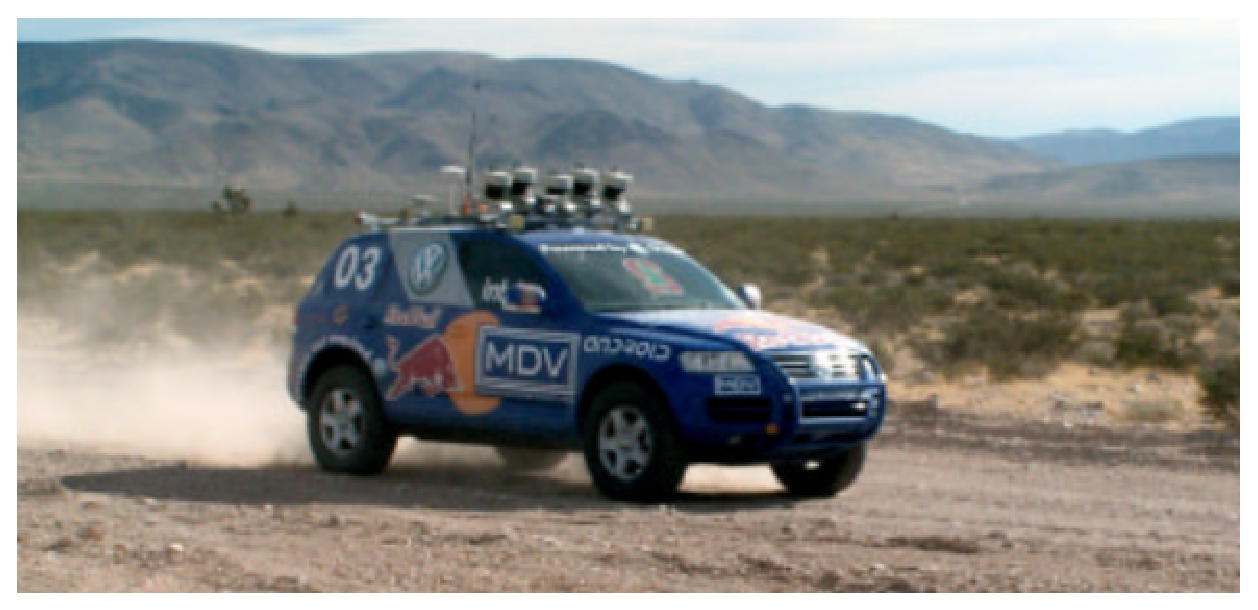
\includegraphics[height=3cm]{imgs/Stanley.eps}
		}
		\subfloat[\label{subfig:boss}]{%
			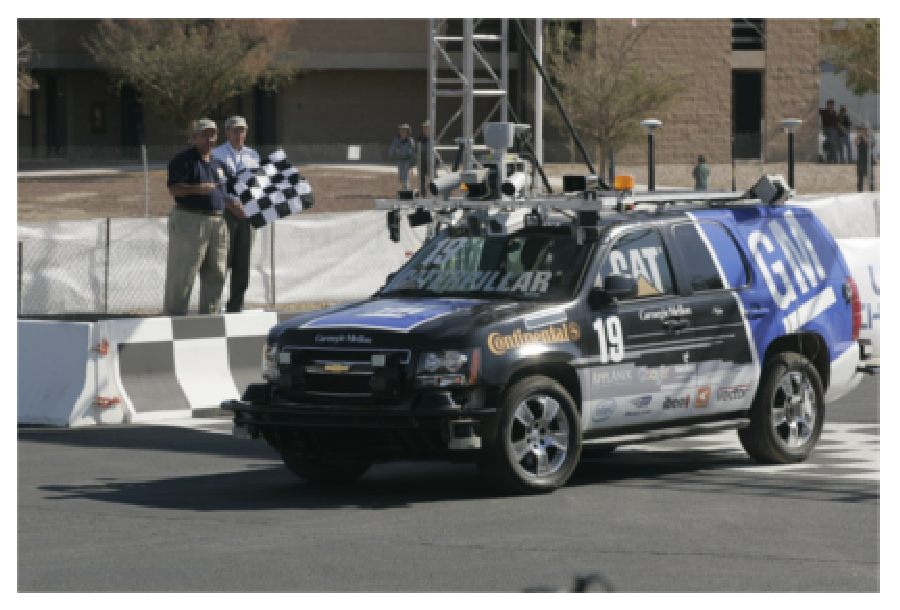
\includegraphics[height=3cm]{imgs/Boss_DARPA_urban_challenge.eps}
		}
	}
	\caption{The winning robots from the 2005 \ac{DARPA} Grand Challenge and 2007 Urban Challenge. ~\protect\subref{subfig:stanley} shows Stanford's Stanley at the 2005 \ac{DARPA} Grand Challenge (Image from \cite{Thrun2006}), ~\protect\subref{subfig:boss} shows Carnegie Mellon's BOSS at the 2007 \ac{DARPA} Urban Challenge (Image from \cite{Urmson.2008}).}\label{fig:darpa_chal}
\end{figure}

The technology developed for the \ac{DARPA} challenges formed the basis for commercial \ac{ADAS}, which have seen rapid progress since then and gradually made their way into series-production vehicles.
There exists a large variety of commercial systems, like e.g. \ac{ACC} or intelligent parking assistance systems, modern vehicles are already equipped with.
These systems have the potential to increase comfort and safety in road traffic and, in the long run enable fully autonomous driving (cf. Level 5 in Table \ref{tab:autonomy_levels}).
On the other hand, many research teams and initiatives were spawned or inspired from these competitions and continued their research work after the \ac{DARPA} Challenges.
Many researchers involved in the winning teams continued their research within Google's self-driving car project, which started in 2009 and evolved into the Spin-Off company Waymo \cite{Waymo} in 2016.
Another research team continuing their efforts after the \ac{DARPA} challenges is the Annieway team \cite{Annieway}.
One of their major contributions is the release and maintenance of the KITTI vision benchmark suite \cite{Geiger2013a}, a publicly available data set containing data from various test drives in the city of Karlsruhe, rural areas as well as highways focusing on providing real world data for vision tasks like stereo, optical flow and 3D object detection and tracking.

The main research goal after the \ac{DARPA} Challenges was to develop automated driving with off-the-shelf sensors \cite{Furgale2013}.
As this thesis focuses on environmental modeling in context of autonomous driving, this section presents research from this field like road detection and modeling (Sec. \ref{subsec:lane}), object detection (Sec. \ref{subsec:obj_detect}) and tracking (Sec. \ref{subsec:obj_track}) as well as sensor fusion (Sec. \ref{subsec:sensor_fusion}) while other aspects like localization \cite{Levinson2010, Thrun2005}, path planning (\todo{citation}) and motion control (\todo{citation}) are neglected.

\subsection{Knowledge Representation}
\label{subsec:knowledge_representation}

As a consequence of increasing complexity of \ac{ADAS} applications, the number of sensors mounted in modern vehicles has grown in recent years and is likely to grow even further in the near future to cover the vehicle's surrounding as completely as possible.
Another factor that leads to an increasing number of sensors in automotive context are safety considerations, which demand for redundancy in the overall setup to ensure functionality even in case of failure of one sensor.
Therefore, automated vehicles need to have a way to combine information from multiple sensor sources.
In the literature, the distinction between different approaches is typically made based on the level at which sensory data is combined \cite{Elfring2016}.
The two main classes of approaches are mostly referred to as \emph{low-level} and \emph{high-level} sensor fusion.
By \emph{low-level} sensor fusion, we mean that raw, previously unprocessed sensor measurements are combined in a coherent representation fur further processing.
In contrast, the goal of \emph{high-level} sensor fusion is to combine preprocessed tracks or features, that have been extracted from raw sensor measurements by each individual (smart) sensor unit.

\subsubsection{Representations for low-level sensor fusion}
\begin{figure*}[t!]
	\centering
	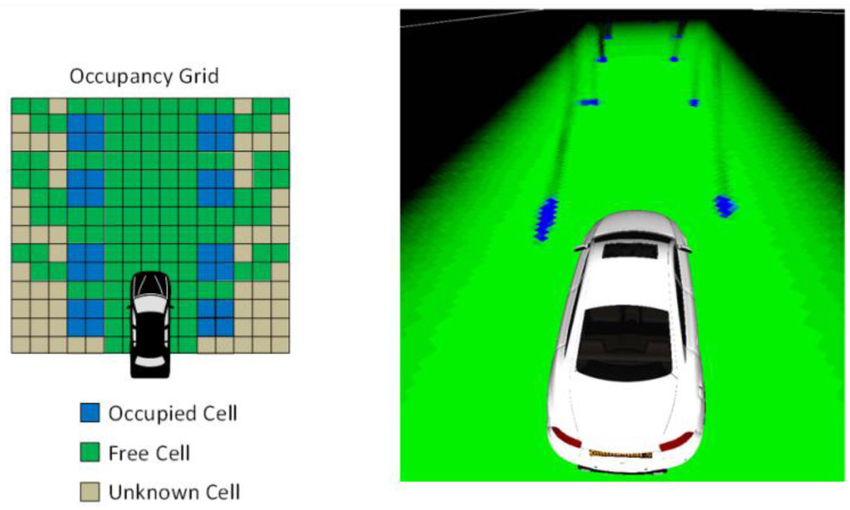
\includegraphics[width=0.95\textwidth]{imgs/occupancy_grid_principle.png}
    \caption{Occupancy-grid visualization for low-level sensor fusion. The left part depicts the principle of occupancy-grids, whereas the right part shows a real world example. Image source \cite{Hohm2014}}
	\label{fig:occupancy-grid}
\end{figure*}

One of the most widely used representations to combine low-level sensory data in robotics is an occupancy-grid map.
This representation is widely used for mobile robot localization \cite{Thrun2005}, but there is also a substantial amount of research regarding occupancy-grids regarding automotive environment modeling  \cite{Tanzmeister2014, Steyer2018}.
The left part of fig.~\ref{fig:occupancy-grid} visualizes the principles of occupancy-grids, whereas the right part shows a real world example from automotive context.
An occupancy-grid divides the represented space in discrete cells, which can take on different occupancy values (e.g., free, occupied or unknown).
The basic assumptions for this representation are that the world is static at each time step and that each cell can have exactly one occupancy value, i.e., one cell is for example completely occupied or completely free.
Therefore, an occupancy-grid is a well-suited representation for range sensors such as \ac{RADAR} or \ac{LIDAR} sensors.
While static occupancy-grid maps are mainly used for localization and \ac{SLAM} applications, there are also approaches to estimate dynamic parameters such as orientation and velocity within the grid to model dynamic environments \cite{Tanzmeister2014}.
The incoming raw sensory data is typically combined through some sort of probabilistic (Bayesian) filter algorithm such as Kalman- \cite{Kalman1960} or particle-filters \cite{Gordon1993}.
One of the main advantages of such a representation is that it is able to incorporate raw, unprocessed sensory data and that the discretization steps as well as the size of the cells can be chosen as fine-grained as the application demands.
Furthermore, it is a natural and precise way to model and represent the free, traversable space around the robot.
On the other hand, occupancy-grids have rather high requirements regarding memory and computational resources.
Additionally, the representation contains no information about type or properties of the obstacles that lead to cells being occupied.
Finally, in contrast to higher-level, more abstract representations, it can be more complex to incorporate sensor modalities other than range finders such as vision sensors.

\subsubsection{Representations for high-level sensor fusion}
In contrast to the low-level sensor fusion representation approaches described previously, high-level sensor fusion typically refers to sensory data being fused, that has already been preprocessed though some sort of temporal filtering.
This usually happens at \emph{tracked objects} level, i.e., object lists provided by individual sensor units each applying their own temporal filtering or tracking based on the data they receive.
To actually combine this sort of information, Bayesian filter approaches similar to the ones mentioned previously could be applied. 
However, such filters assume uncorrelated data and thus may deliver overconfident or diverging estimates since objects provided by different filters coming from several sensor sources are in fact correlated due to phenomena such as shared modeling assumptions, common noise acting on the objects being tracked or measurements arriving out of sequence.
Therefore, more advanced track-to-track fusion algorithms need to be used for high-level sensor fusion \cite{Tian2010, Aeberhard2012}.
These methods typically differ regarding the amount of knowledge they assume to be known about the correlations between the tracks.

The main advantages of high-level sensor fusion are that the amount of transferred data is lower compared to low-level fusion due to the hierarchical structure of the estimation framework.
Furthermore, as many sensors already employ on-board processing and provide data only at tracked object level, implementation of high-level fusion often does not require in-depth knowledge of the sensor characteristics.
This gives a more abstract interface and allows for easier replacement of individual sensor units in case the overall setup changes.
On the other hand, high-level fusion ignores potentially useful information, as it might be discarded at sensor level before the fusion is performed.
In summary, high-level sensor fusion is arguably the most popular and frequently used approach for combining information from different sensor sources in automated driving.
The objects are typically represented as "point objects" using a unique identifier and a state vector for dynamic information such as position, velocity and acceleration.
For certain application types, additional information such as the objects' size, shape and type need to be known (e.g., pedestrians have different dimensions and motion characteristics compared to trucks or vehicles).
For other objects of interest (e.g., traffic signs or traffic lights), color and shape information might be important.
While this type of representation is compact and abstract enough and thus well-suited for high-level fusion, the content and thus the represented values might vary depending on the sensor providing the information.
Therefore, achieving a unified representation across different sensor modalities can become a challenging problem.

\subsubsection{Other representations}
Representation approaches other than the aforementioned ones are rather rarely used in an automotive context.
Although semantic and structured information will grow more important with the advent of numerous and increasingly complex machine learning driven assistant systems, representations that are able to capture and manipulate such information are still hardly used in vehicle context.
One example of an alternative knowledge representation approach is the work presented in \cite{Yamazaki2016}, where the authors use symbolization, a language modeling technique, to obtain semantic descriptions of driving scenes.

\subsection{Driving Context Classification}
For the specific task of recognizing the current driving context, there have been early approaches using statistical pattern recognition based solely on the ego-vehicle's dynamics \cite{Engstrom2001} or on fusion with camera data \cite{Hauptmann1996}.
The key difference to previous work is that our approach employs cognitive modeling techniques, which allows us to use symbolization as well, but also to combine it with the benefits of neural networks.

\subsection{Object Detection and Classification}
\label{subsec:obj_detect}
\subsection{Behavior Analysis}
\label{subsec:behav_analysis}

\begin{figure*}[t!]
	\centering
	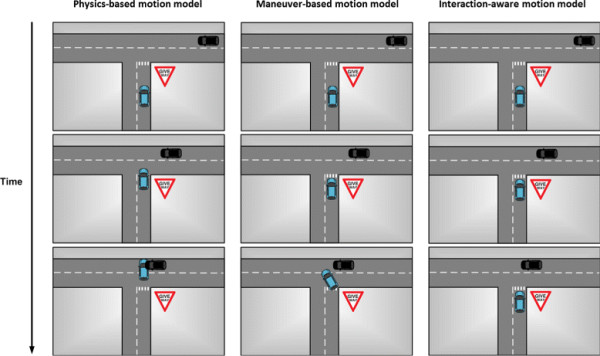
\includegraphics[width=0.95\textwidth]{imgs/examples_motion_prediction_models.jpg}
	\caption{Examples visualizing different modeling approaches for motion prediction in automotive context, Image source \cite{Lefevre2014}}
	\label{fig:examples_motion_prediction_types}
\end{figure*}
Predicting future behavior and positions of other traffic participants from observations is essential for collision avoidance and thus safe motion planning, and needs to be solved by human drivers and automated vehicles alike to reach their desired goal.
However, future positions of vehicles not only depend on each vehicle's own past positions and dynamics like  velocity and acceleration, but also on the behavior of the other traffic participants in the vehicle's surroundings.
Motion prediction for intelligent vehicles in general has seen extensive research in recent years, as it is a cornerstone for collision-free automated driving. \cite{Lefevre2014} classify such prediction approaches into three categories, namely \emph{physics-based}, \emph{maneuver-based} and \emph{interaction-aware}, depending on their level of abstraction.
\todo[inline]{add phrase referring to fig. \ref{fig:examples_motion_prediction_types}}
\emph{Physics-based} and \emph{maneuver-based} motion models consider the law of physics and the intended driving maneuver respectively as the only influencing factors for future vehicle motion and ignore inter-dependencies between the motion of different vehicles.
\todo[inline]{maybe add some more info on those motion models}
There exist a growing number of different \emph{interaction-aware} approaches to account for those dependencies and mutual influences between traffic participants or, more generally, agents in the scene.
Probabilistic models like cost maps \cite{Bahram2016} account for physical constraints on the movements of the other vehicles.
Classification approaches categorize and represent scenes in a hierarchy \cite{Bonnin2012} based on the most generic ones to predict behavior for a variety of different situations.
Data-driven approaches to behavior prediction mainly rely on \ac{LSTM} neural network architectures, which have proven to be a powerful tool for sequential data analysis.
\cite{Alahi2016} model interactions in the learning network architecture by introducing so-called social-pooling layers to connect several \acp{LSTM} each predicting one agent at a time.
\cite{Deo2018a} adapted the combination of \ac{LSTM} networks for encoding vehicle trajectories and (convolutional) social-pooling layers to account for interactions to vehicle prediction in highway situations.
\cite{Altche2018} use a \ac{LSTM} network as well, but they account for interaction by including distances between the target vehicle and other agents directly in the training data rather than adapting the network architecture.
A similar approach is proposed in \cite{Deo2018}, but the authors combine \ac{LSTM} networks with an additional maneuver classification network to predict future vehicle motion.
One issue in data-driven approaches to behavior prediction accounting for relations between agents is that the number of other vehicles is variable.
If information about vehicles other than the target are encapsulated in the input of the neural network, typically a specific number of other vehicles of interest are manually chosen a priori to avoid this issue \cite{Altche2018, Deo2018}.
If the information about other vehicles is encapsulated in the network architecture, it might be necessary to train several networks depending on the situation at hand.

\section{Summary}
\label{sec:related_work_summary}

%----------------------------------------------------------------------------------------------------------
\chapter{Theoretical background}%
\label{chap:introduction_to_vsas}
%----------------------------------------------------------------------------------------------------------

In this chapter, we present the theoretical background and mathematical formalism needed as basis for later chapters.
We introduce \acfp{VSA}, describe their most important properties and present proofs where relevant for this thesis.
We proceed with one particular instantiation of \ac{VSA}, the \acf{SPA}, and present more specific properties, which do not necessary hold for all \acp{VSA}.
Additionally, we give a brief introduction to the theory of the \acf{NEF}, a set of mathematical tools enabling the implementation of the \ac{SPA} in \acp{SNN}.
Then, we shift our focus to cognitive modeling based on such vector representations keeping it as generic as possible without particular attention on the \ac{SPA}. 
We show several approaches to generate vector vocabularies, which form the basis of more complex structured representations built from them using the \ac{VSA}'s algebraic operations.
Bringing all of the presented tools together, we show how the \ac{NEF} can be used to implement vector representations, which have been generated using the \ac{SPA}, in a spiking neuron substrate.

%----------------------------------------------------------------------------------------------------------
\section{Mathematical properties of \aclp{VSA}}
\label{sec:math_prop_vsas}
%----------------------------------------------------------------------------------------------------------

The term \acp{VSA} - first coined by \textcite{Gayler2003} - refers to a class of similar approaches for cognitive modeling making use of distributed representations.
The basic idea behind all of those approaches is to represent structure, i.e., cognitive concepts, symbols or language, in a high-dimensional vector space by mapping each entity to be represented to a (possibly random) vector.
One of the most important properties of high-dimensional vector spaces enabling this kind of representation is the fact that two high-dimensional random vectors are likely to be dissimilar.
In the following, we will show what we mean by fuzzy terms like \emph{dissimilar} or \emph{likely} and provide more precise statements.

One main requirement in the context of cognitive modeling is the ability of the modeling framework to address the binding problem \parencite{Treisman1999}.
\textcite{Jackendoff2002} phrases this as the problem of \enquote{combining independent bits into a single coherent percept}.
One strength of \acp{VSA} is that they offer the possibility to manipulate their entities (i.e., vectors) through algebraic operations, usually at least one \emph{addition-like} and \emph{multiplication-like} operation each.
Typically, the multiplication operation is used for binding different representations into a new vector.
This operation, depending on the vector representation, is constructed with some desirable properties in mind (see Definition~\ref{def:binding}).
A first attempt on using a multiplication operation for binding vectors was done by \textcite{Smolensky1990} using the tensor product.
The major drawback of this approach is exploding dimensionality of the tensor product.
For finite dimensional vector spaces  $V$ and $W$ of dimensions $n$ and $m$, the tensor space $V \otimes W$ is a vector space of dimension $n\cdot m$.
As a consequence, each binding operation $v\otimes w$ for vectors $ \mathbf{v} \in V, \mathbf{w} \in W$ would increase the dimension of the representational space, which is computationally unfeasible and leads to poor scaling.
This lead researchers to define several slightly different multiplication or binding operations, depending on the underlying numerical structure.
The most prominent examples are element-wise multiplication in the \ac{MAP}-architecture proposed by \textcite{Gayler1998}, the XOR-operation in \acp{BSC} proposed in \textcite{Kanerva2000, Kanerva2009} as well as circular convolution \acp{HRR} proposed in \textcite{Plate1991, Plate1994}.

\begin{defn}
	\label{def:VSA}
	Let $N \subseteq K$ be a subset of some number field $K$ (i.e., a set of numbers) and $D \in \mathbb{N}$ a natural number.
	Furthermore, let
	\[V_{D}(N)=\{ \mathbf{x}=\left(x_{0}, \cdots, x_{D-1}\right)  | x_{i} \in N\} \subseteq K^{D}\]
	be the set of all $D$-tuples with entries in $N$.
	Let
	\begin{align*}
		&\abb{\oplus}{V_{D}(N) \times V_{D}(N)}{K^{D}}{( \mathbf{v}, \mathbf{w})}{\oplus( \mathbf{v}, \mathbf{w}) =: \mathbf{v}\oplus \mathbf{w}}, \\
		&\abb{\varoast}{V_{D}(N) \times V_{D}(N)}{K^{D}}{( \mathbf{v}, \mathbf{w})}{\varoast( \mathbf{v}, \mathbf{w}) =: \mathbf{v}\varoast \mathbf{w}}
	\end{align*}
	be functions with $\oplus$ following the rules of ordinary addition - namely commutativity, associativity, existence of a neutral element and existence of inverse elements - and for any elements $ \mathbf{u}, \mathbf{v}, \mathbf{w} \in V_{D}(N)$
	\[ \mathbf{u} \varoast ( \mathbf{v} \oplus \mathbf{w}) = \mathbf{u} \varoast \mathbf{v} \oplus \mathbf{u} \varoast \mathbf{w}.\]
	If there is furthermore a distinct element $\pmb{1} \in V_{D}(N)$ with
	\[ \mathbf{v} \varoast \pmb{1} = \pmb{1} \varoast \mathbf{v} = \mathbf{v}\]
	for any $ \mathbf{v} \in V_{D}(N)$ and a function $\abbil{\phi}{V_{D}(N) \times V_{D}(N)}{\left[-1,1\right]}$, we call $(V_{D}(N), \varoast, \oplus, \phi)$ a \emph{\acrfull{VSA}} of dimension $D$.
	The function $\phi$ is called a \emph{measure of similarity}.
	If $N$ is a subset of the real or complex numbers, i.e., $N \subset \mathbb{R}$ or $N \subseteq \mathbb{C}$, we call any \ac{VSA} $\left(V_{D}(N), \varoast, \oplus, \phi\right)$ \emph{continuous}.
\end{defn}
Although the set $V_{D}(N)$ might not be a vector space in the strict mathematical sense (in most cases it is at least a subset of a vector space), we will refer to its elements as \emph{vectors}.
%The metric in definition~\ref{def:VSA} is needed as measure of similarity between vectors.
Before we proceed in deriving some important properties of \acp{VSA}, we present some of the most prominent examples.

\begin{ex} \aclp{VSA}
	\label{ex:VSAs}
	\begin{enumerate}
		\item The first example of a \ac{VSA} is \acfl{BSC}.
            \textcite{Kanerva2009} restricts the elements of his vectors to binary values, i.e., $N=\{0,1\} = \mathbb{F}_{2}$.
		The operations $\varoast$ and $\oplus$ in this case are the XOR-function and a thresholded sum respectively.
		With $ \mathbf{v}_{i} = \left(v_{i 0}, \cdots, v_{i D-1}\right) \in V_{D}(N)$ and  $i \in \{1, \cdots, n\}$, the operation $\oplus$ is usually defined in the following way
		\begin{align*}
			\mathbf{v}_{1} \oplus \cdots \oplus \mathbf{v}_{n} =: &\mathbf{x} = \left(x_{0}, \cdots, x_{D-1}\right) \textrm{ with } \\
			&x_{j}:= \begin{cases}
				1 & \sum\limits_{i=1}^{n} v_{ij} \geq \frac{n}{2} \\
				0 & \sum\limits_{i=1}^{n} v_{ij} < \frac{n}{2}
			\end{cases}.
		\end{align*}
		This definition ensures, that the results of the addition operation $\oplus$ remain binary.
		Usually, a normalized Hamming distance
		\[
		\phi( \mathbf{v}, \mathbf{w}) := 1 - \frac{2}{D} \left| \{ v_{i} \neq w_{i} | i \in \{0, \cdots, D-1\} \} \right|
		\]
		is used as a measure of similarity in this architecture.
		\acp{BSC} have some interesting properties compared to other \acp{VSA}:
		The neutral element for both operations $\varoast$ and $\oplus$ is the vector $\pmb{0} := \left(0, \cdots, 0\right)$, while all vectors are self-inverse regarding the multiplication operation $\varoast$, i.e., $ \mathbf{v} \varoast \mathbf{v} = \pmb{0}$ for any $ \mathbf{v} \in V_{D}(N)$.

		\item The first example of a \ac{VSA} in continuous space is the \acrfull{MAP} architecture proposed by \textcite{Gayler1998} with $N \subseteq \mathbb{R}$ and the cosine similarity as measure of similarity
		\[
		\phi( \mathbf{v}, \mathbf{w}) = \frac{ \mathbf{v} \cdot \mathbf{w}}{\norm{ \mathbf{v}}\norm{ \mathbf{w}}}=\cos(\theta),
		\]
		with $\theta$ being the angle between the vectors $ \mathbf{v}, \mathbf{w} \in V_{D}(N)$.
		The operations $\varoast$ and $\oplus$ are simply element-wise multiplication and addition with neutral elements $\pmb{1}=\left(1, \cdots, 1\right)$ and $\pmb{0} := \left(0, \cdots, 0\right)$ respectively.

		\item Another example of a \ac{VSA} in continuous space is \acfl{HRR} proposed by \textcite{Plate1991}.
		The main difference compared to the \ac{MAP} architecture is, that \textcite{Plate1994} in general allows complex vector values, i.e., $N \subseteq \mathbb{C}$ and uses a different multiplication operation $\varoast$: circular convolution.
		For any two vectors $ \mathbf{x}, \mathbf{y} \in V_{D}(N)$, circular convolution $\varoast$ is defined as
		\begin{align*}
			\mathbf{z} = \mathbf{x} \varoast \mathbf{y} \qquad \textrm{ with } z_{j} := \sum_{k=0}^{D-1} x_{k}y_{(j-k)\Mod{D}}.
		\end{align*}
        \begin{figure}[t!]
            \centering
            \begin{tikzpicture}
            \Vertex[color=gray!70, opacity=0.4, size=0.5, label=$x_0$, fontsize=\large, position=left]{x0y0} 
            \Vertex[y=2,style={color=white}, size=0.5,label=$y_0$, fontsize=\large, position=below, distance=1cm]{y0} 
            \Vertex[x=-1,y=-1,style={color=white}, size=0.5, label=$z_0$, fontsize=\large, position=center, distance=0.1cm]{z0} 
            \Vertex[style={color=white}, opacity=1.0, size=0.01, x=2, y=2, label=$y_1$, fontsize=\large, position=below, distance=1cm]{y1} 
            \Vertex[x=-1,y=-3,style={color=white}, size=0.5, label=$z_1$, fontsize=\large, position=center, distance=0.1cm]{z1} 
            \Vertex[style={color=white}, size=0.5, x=4, y=2, label=$y_2$, fontsize=\large, position=below, distance=1cm]{y2} 
            \Vertex[x=-1,y=-5,style={color=white}, size=0.5, label=$z_2$, fontsize=\large, position=center, distance=0.1cm]{z2} 
            \Vertex[x=2,color=gray!70, opacity=0.4, size=0.5]{x0y1}
            \Vertex[x=4,color=gray!70, opacity=0.4, size=0.5]{x0y2}
            \Vertex[y=-2,color=gray!70, opacity=0.4, size=0.5, label=$x_1$, fontsize=\large, position=left]{x1y0} 
            \Vertex[x=2,y=-2,color=gray!70, opacity=0.4, size=0.5]{x1y1}
            \Vertex[x=4,y=-2,color=gray!70, opacity=0.4, size=0.5]{x1y2}
            \Vertex[y=-4,color=gray!70, opacity=0.4, size=0.5, label=$x_2$, fontsize=\large, position=left]{x2y0} 
            \Vertex[x=2,y=-4,color=gray!70, opacity=0.4, size=0.5]{x2y1}
            \Vertex[x=4,y=-4,color=gray!70, opacity=0.4, size=0.5]{x2y2}
            \Edge(x2y1)(x1y2)
            \Edge[Direct](x0y0)(z0)
            \Edge[Direct](x1y0)(z1)
            \Edge[Direct](x2y0)(z2)
            \Edge(x1y1)(x2y0)
            \Edge(x0y2)(x1y1)
            \Edge(x0y1)(x1y0)
            \Edge(y1)(x0y0)
            \draw [line width=1.5pt, color=black!75] (5,-1) edge[out=45, in=45] (2,2);
            \draw [-<,>=latex,line width=1.5pt, color=black!75] (x1y2) edge[out=45, in=45] (5,-1);
            \draw [line width=1.5pt, color=black!75] (1.9,1.9) edge[out=45, in=45] (x0y0);
            \draw [line width=1.5pt, color=black!75] (3,1) edge[out=45, in=45] (x0y1);
            \draw [line width=1.5pt, color=black!75] (6,-2) edge[out=45, in=45] (3,1);
            \draw [line width=1.5pt, color=black!75] (x0y2) edge[out=45, in=45] (4.5,0.5);
            \draw [line width=1.5pt, color=black!75] (x2y1) edge (1,-5);
            \draw [line width=1.5pt, color=black!75] (x2y2) edge (3,-5);
            \draw [->,>=latex,line width=1.5pt, color=black!75] (x2y2) edge (5.5,-2.5);
            \draw [line width=1.5pt, color=black!75]  (5.4,-2.6) edge (6,-2) ;
            \node [text width=6cm, align=center] at (10,-1) {\Large
                    $\begin{aligned}
                        \mathbf{z} &= \mathbf{x} \varoast \mathbf{y}\\
                        z_0 = x_0y_0 &+ x_2y_1+x_1y_2\\
                        z_1 = x_1y_0 &+ x_0y_1+x_2y_2\\
                        z_2 = x_2y_0 &+ x_1y_1+x_0y_2
                    \end{aligned}$ }; 
        \end{tikzpicture}
        \caption{Visualization of circular convolution as compressed outer product for $3$-dimensional vectors. Image adapted from \textcite{Plate1994a}.}
        \label{fig:circ_conv}
        \end{figure}
		The neutral element regarding circular convolution is $\pmb{1} = \left(1, 0, \cdots, 0\right)$.
		One important property of this operation is the fact that circular convolution can efficiently be computed using the \ac{DFT}.
		The \ac{DFT} is defined as the function
        \begin{equation}
        \label{eq:dft}
		\abb{\ac{DFT}}{\mathbb{C}^{D}}{\mathbb{C}^{D}}{ \mathbf{x}}{\left(\sum_{j=0}^{D-1} x_{j} \zeta_{D}^{-jk} \right)_{k=0}^{D-1}} \qquad \textrm{ with } \zeta_{D} = \exp\left( \frac{i 2 \pi}{D} \right).
        \end{equation}
		Similarly, the \ac{IDFT} is defined as the function
        \begin{equation}
        \label{eq:inv_dft}
		\abb{\ac{IDFT}}{\mathbb{C}^{D}}{\mathbb{C}^{D}}{ \mathbf{x}}{\left( \frac{1}{D} \sum_{j=0}^{D-1} x_{j} \zeta_{D}^{jk} \right)_{k=0}^{D-1}}.
        \end{equation}
        From the convolution theorem \parencite[see][Chap. 6]{Bracewell2000} we know, that we can calculate the circular convolution of any two vectors $ \mathbf{v}, \mathbf{w} \in V_{D}(N)$ by
        \begin{equation}
        \label{eq:conv_with_dft}
		\mathbf{v} \varoast \mathbf{w} = \ac{IDFT}\left(\ac{DFT}( \mathbf{v}) \odot \ac{DFT}( \mathbf{w}) \right),
        \end{equation}
		with $\odot$ denoting element-wise multiplication in this case.
		This induces that circular convolution obeys the same rules (commutativity and associativity) as element-wise multiplication, as both operations are the same except for a change of basis.
	\end{enumerate}
\end{ex}
As mentioned earlier, one of the most important features of (high-dimensional) \acp{VSA} is the fact that two random vectors are likely to be dissimilar.
We will derive this result in the following Theorem.
\begin{theorem}
	\label{theorem:VSA_cossim_distribution}
	Let $\left(V_{D}(N), \varoast, \oplus, \phi \right)$ a \acl{VSA}.
    For two randomly chosen vectors $ \mathbf{v}, \mathbf{w} \in V_{D}(N)$, the distribution of the similarity $\phi\left( \mathbf{v}, \mathbf{w}\right)$ is a version of the beta-distribution $\mathcal{B}_{\frac{D-1}{2},\frac{D-1}{2}}$ scaled and shifted to the interval $\left[-1,1\right]$ with mean $\mu=0$ and variance $\sigma^2=\frac{c^2}{D}$ up to a constant $c$.
    The standardized distribution trends towards a normal distribution with growing $D$.
\end{theorem}
\begin{proof}
	We will only give the proof of this Theorem for real valued \acp{VSA}, i.e., $N \subseteq \mathbb{R}$ and $\phi$ as the cosine similarity.
	Without loss of generality, we assume the vectors $ \mathbf{v}, \mathbf{w}$ picked randomly from the unit sphere $\mathbb{S}^{D-1} = \{ \mathbf{v} \in \mathbb{R}^{D} | \norm{ \mathbf{v}} = 1 \}$, as we can simply normalize the vectors by $\frac{ \mathbf{v}}{\norm{ \mathbf{v}}}$.
    Since binary \acp{VSA} can be associated with a euclidean sphere as well, the same result can be proven for those architectures with similar arguments \parencite[see][for details]{Kanerva1988}.
	Due to symmetry of the unit sphere $\mathbb{S}^{D-1}$, we can furthermore - again without loss of generality - choose one vector as a unit vector, i.e., $ \mathbf{w}=\left(1, 0 , \cdots, 0\right)$.
	Thereby, the cosine similarity for $ \mathbf{v}=\left(v_{0}, \cdots, v_{D-1}\right)$ is given by $\phi\left( \mathbf{v}, \mathbf{w}\right) = v_{0}$
	By fixing one coordinate, we get the constraint $\sum_{i=1}^{D-1} v_{i}^{2} = 1-v_{0}^{2}$, which is equivalent to a lower dimensional sphere $\mathbb{S}^{D-2}$ with radius $\sqrt{1-v_{0}^2}$.
	Hence, the cosine similarity $\phi\left( \mathbf{v}, \mathbf{w}\right)=:x$ is proportional to the surface of a conical frustum constructed from $\mathbb{S}^{D-2}$ with radius $\sqrt{1-x^{2}}$, slope $\frac{1}{\sqrt{1-x^{2}}}$ and some height $h$, i.e., the density function is proportional to
	\[
	f_{\phi( \mathbf{v}, \mathbf{w})}(x) \propto \frac{\sqrt{1-x^{2}}^{(D-2)}}{\sqrt{1-x^{2}}} h \propto \left(1-x^{2}\right)^{\frac{D-3}{2}}.
	\]
	Substituting $x=2u-1$, we get
	\[
	\left(1-\left(2u-1\right)^{2}\right)^{\frac{D-3}{2}} \propto \left(u-u^2\right)^{\frac{D-3}{2}} = \left(u \left(1-u\right)\right)^{\frac{D-3}{2}} = u^{\left(\frac{D-1}{2}-1\right)} \left(1-u\right)^{\left(\frac{D-1}{2}-1\right)},
	\]
	which is the density function of the beta distribution $\mathcal{B}_{\frac{D-1}{2},\frac{D-1}{2}}$.
	Thus, the cosine similarity is also beta distributed, but scaled and shifted to the interval $\left[-1,1\right]$ by $x=2u-1$.
    
	For $\alpha=\beta=\frac{D-1}{2}$, the mean of the beta distribution is $\tilde{\mu}=\frac{1}{2}$. Applying the substitution, we get the mean of the shifted distribution $\mu = 2\tilde{\mu }-1 = 0$.
    
	Making use of the simplification that the distribution of similarity is the same as the distribution in the first coordinate, the variance is given by the expected value of the square value of the first coordinate, i.e., $\mathbb{E}(v_{0}^{2})$.
	Since all coordinates are identically distributed, we get
	\[
	\mathbb{E}(v_{0}) = \frac{1}{D} \sum_{i=0}^{D-1} \mathbb{E}(v_{i}^2)= \frac{1}{D} \underbrace{\mathbb{E}\left(\sum_{i=0}^{D-1} v_{i}^2\right)}_{=:c^2}=\frac{c^2}{D}.
	\]
	Hence, the variance of the distribution of the cosine similarity is $\sigma^2=\frac{c^2}{D}$.
	In the particular case of the unit sphere $\mathbb{S}^{D-1}$, we get $c^{2}=1$ and a variance of $\sigma^2=\frac{1}{D}$.
    
	To see the convergence behavior of the standardized distribution, we look at the logarithm of its density function %$f_{\phi(v,w)}\left(\frac{x}{\sqrt{D}}\right)$
	\begin{equation}
	\label{eq:log_dens}
	\log\left(f_{\phi(v,w)}\left(\frac{x}{\sqrt{D}}\right)\right) = \frac{D-3}{2}\log\left(1-\frac{x^2}{D}\right) + C.
	\end{equation}
	Using the Taylor series approximation of the logarithm, equation~\eqref{eq:log_dens} transforms to
	\begin{align*}
		\log\left(f_{\phi(v,w)}\left(\frac{x}{\sqrt{D}}\right)\right) &= \frac{D-3}{2}\left(-\frac{x^2}{D} + \frac{x^4}{4D} \pm \ldots \right) + C = -\frac{1}{2}x^2 + \frac{3}{2D}x^2 + \mathcal{O}\left(\frac{x^4}{D}\right)  + C  \\
		&\longrightarrow -\frac{1}{2}x^2 + C = \log\left(f_{\mathcal{N}}\left(x\right)\right) \textrm{ for } D \longrightarrow \infty.
	\end{align*}
	Hence, with growing $D$ the standardized distribution of the cosine similarity trends to a normal distribution.
\end{proof}
Theorem~\ref{theorem:VSA_cossim_distribution} states that the probability of finding two random, non-orthogonal vectors in a \ac{VSA} decreases with growing vector dimension.
\begin{figure}[t]
    \centering
    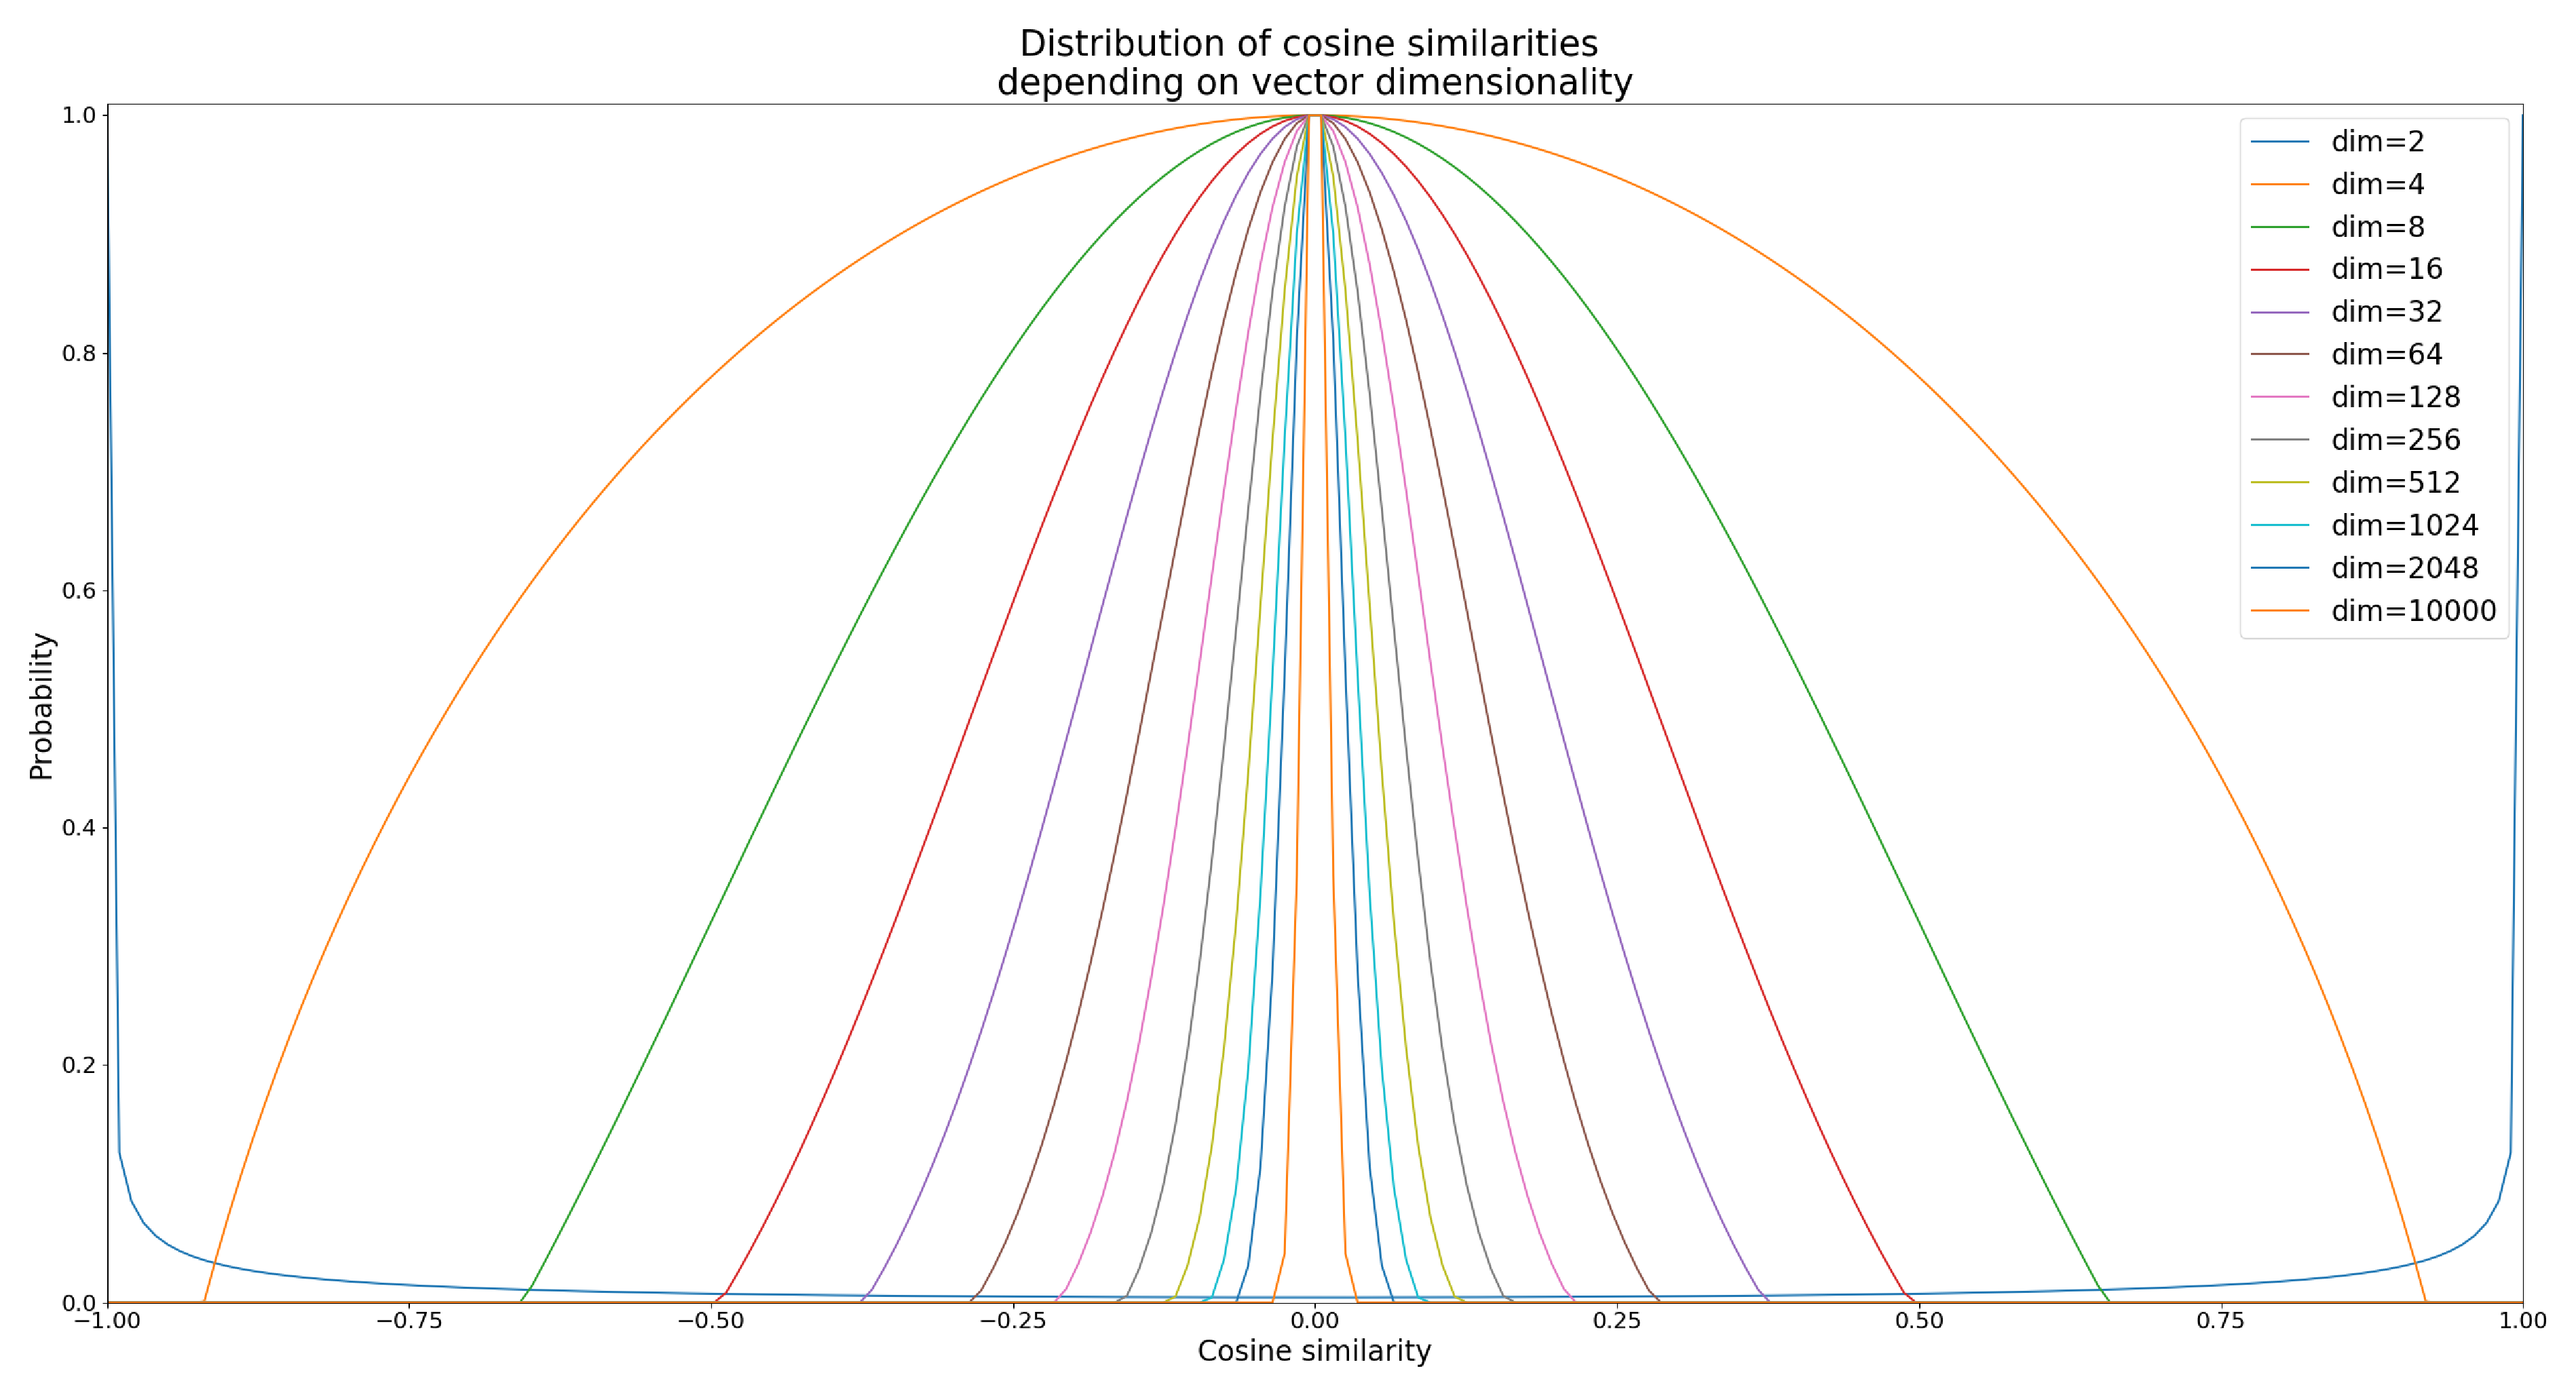
\includegraphics[width=1.\linewidth]{imgs/distributions_cosine_sims.eps}
    \caption{Visualization of the distribution of the cosine similarity between two randomly chosen vectors depending on their dimension.}
    \label{fig:distributions_cosine_sims}
\end{figure}
Figure~\ref{fig:distributions_cosine_sims}, which shows the probability distributions of cosine similarity for different vector dimensions, illustrates this result.
Furthermore, Theorem~\ref{theorem:VSA_cossim_distribution} allows us to give a more formal definition of the term \emph{dissimilar}.
\begin{defn}
	\label{def:similar}
	Let $(V_{D}(N), \varoast, \oplus, \phi)$ be a \acrfull{VSA} of dimension $D$ and $c \in \mathbb{N}$ a constant. We call any two vectors $ \mathbf{v}, \mathbf{w} \in v_{d}(n)$ \emph{dissimilar}, if
    \begin{equation}
    \label{eq:dissmilar}
	\left| \phi( \mathbf{v}, \mathbf{w}) \right| \leq \epsilon, \textrm{ with } \epsilon:=\tfrac{c}{\sqrt{D}}.
    \end{equation}
	Analogously, we call any two vectors $ \mathbf{v}, \mathbf{w} \in V_{D}(N)$ \emph{similar}, if	$\left| \phi( \mathbf{v}, \mathbf{w}) \right| > \epsilon$.
	Similar vectors are denoted by $ \mathbf{v} \approx \mathbf{w}$. 
\end{defn}
Definition~\ref{def:similar} can also be stated as follows: we consider any two vectors similar, if their similarity is higher than what we would expect from two randomly chosen vectors.
Therefore, we make use of the fact that for growing dimension $D$ the cosine similarity follows approximately a normal distribution $\mathcal{N}_{\mu, \sigma}$, with $\mu=0$ and $\sigma=\tfrac{1}{\sqrt{D}}$ and the so-called three-sigma-rule.
This rule, which follows from Chebyshev's inequality, states that the probability $\mathbb{P}\left(\mu-3\sigma \leq X \leq \mu+3\sigma \right) \geq 0.95$ for any unimodal distributed random variable $X$.
For normally distributed $X$, we even have
\begin{align*}
	\mathbb{P}\left(\mu-2\sigma \leq X \leq \mu+2\sigma \right) &\approx 0.954 \\
	\mathbb{P}\left(\mu-3\sigma \leq X \leq \mu+3\sigma \right) &\approx 0.997.
\end{align*}
Given Definition~\ref{def:similar}, the probability of two randomly chosen vectors being similar is below \SI{5}{\percent} for $c=2$ and even below \SI{0.3}{\percent} for $c=3$, while the actual numerical interval $\left[-c\sigma, c\sigma\right]$ only depends on the vector dimension $D$.
Hence, we denote the weaker version of Definition~\ref{def:similar} by $\epsilon_{weak} = \tfrac{2}{\sqrt{D}}$ as \emph{weak similarity threshold} and the stronger version by $\epsilon_{strong} = \tfrac{3}{\sqrt{D}}$ as \emph{strong similarity threshold}.
For lower \ac{VSA} dimensions such as $D \leq 50$, it can be beneficial to work with the weak similarity threshold, whereas for higher dimensions the stronger version can be used.

Based on the definition of similarity, we derive criteria for \enquote{good} multiplication functions in \acp{VSA}.
\begin{defn}
	\label{def:binding}
	Let $(V_{D}(N), \varoast, \oplus, \phi)$ be a \acrfull{VSA} of dimension $D$. We call its multiplication function
	\[\abb{\varoast}{V_{D}(N) \times V_{D}(N)}{K^{D}}{( \mathbf{v}, \mathbf{w})}{\varoast( \mathbf{v}, \mathbf{w}) =: \mathbf{v}\varoast \mathbf{w}}\]
	a \emph{binding function} if
	\begin{enumerate}
		\item for any two vectors $ \mathbf{v}, \mathbf{w} \in V_{D}(N)$, the vector $ \mathbf{v} \varoast \mathbf{w}$ is dissimilar to both $ \mathbf{v}$ and $ \mathbf{w}$, i.e.,
		\[
		\left| \phi( \mathbf{v}, \mathbf{v} \varoast \mathbf{w}) \right| \leq \epsilon \textrm{ and } \left| \phi( \mathbf{w}, \mathbf{v} \varoast \mathbf{w}) \right| \leq \epsilon.
		\]
		\item for any vector $ \mathbf{v} \in V_{D}(N)$, there exists a vector $\bar{\mathbf{v}} \in V_{D}(N)$ with $ \mathbf{v} \varoast \bar{\mathbf{v}} \approx \mathbf{1}$. We call $\bar{\mathbf{v}}$ a \emph{pseudo-inverse} element.
		If furthermore $ \mathbf{v} \varoast \bar{\mathbf{v}} = \mathbf{1}$, we call the vector $\bar{\mathbf{v}}$ \emph{exact inverse}.
	\end{enumerate}
\end{defn}
It is worth noting, that all multiplication operations mentioned in Example~\ref{ex:VSAs} fulfill the criteria for binding functions as stated in Definition~\ref{def:binding}.
The first criteria is intended to allow structured representations in \acp{VSA}.
Representations built solely upon an addition function lack a mechanism to impose structure, as the sum of vectors is similar to all summands.
For continuous \acp{VSA}, this result is straightforward due to the linearity of the dot product, but it holds true for \acp{BSC} as well.
Therefore, summing vectors only allows to encode unordered sets of entities.
The property of binding functions to map two vectors to a vector dissimilar to both inputs enables structured representations.

The second criteria of Definition~\ref{def:binding} for binding functions is the basis to decode or recover the individual vector ingredients from structured representations.
The existence of a (pseudo-) inverse element allows the retrieval of $ \mathbf{v}, \mathbf{w} \in V_{D}(N)$ from $ \mathbf{v} \varoast \mathbf{w}$ by
\begin{equation}
\label{eq:retrieval}
\bar{\mathbf{v}} \varoast \left(\mathbf{v} \varoast \mathbf{w}\right) = \underbrace{\bar{\mathbf{v}} \varoast \mathbf{v}}_{\approx \mathbf{1}} \varoast \mathbf{w} = \tilde{\mathbf{w}} \approx \mathbf{w}.
\end{equation}
In case of exact inverse elements, the right hand side of equation~\eqref{eq:retrieval} becomes an exact equality $\tilde{\mathbf{w}}= \mathbf{w}$.
In most cases, however, the result $\tilde{\mathbf{w}}$ is not exactly equal to $ \mathbf{w}$, but similar.
It is this inherent inexactness of most \acp{VSA} that makes them suitable candidates for cognitive modeling \parencite{Eliasmith2013}.
On the other hand, it imposes a functional demand for a clean-up memory.
A clean-up memory is a mechanism, which maps noisy versions of vectors like $\tilde{\mathbf{w}}$ to their exact counterparts, here $ \mathbf{w}$.
Therefore, we need to have a set of vectors, which represent established concepts or symbols the system has knowledge of.

\begin{defn}
	\label{def:clean-up-mem}
	Let $(V_{D}(N), \varoast, \oplus, \phi)$ be a \acrfull{VSA} of dimension $D$ with binding function $\varoast$.
	We call a finite subset $\vartheta \subsetneq V_{D}(N)$ a \emph{vocabulary}.
	A function $\abbil{\gamma}{K^{D}}{\vartheta}$ is called a \emph{clean-up memory}, if
	\begin{enumerate}
		\item for any vector $v\in K^{D}$ we have
		\[
		\phi\left( \mathbf{v}, \gamma(\mathbf{v})\right) > \phi\left( \mathbf{v}, \mathbf{w}\right), \textrm{ for any vector } \mathbf{w} \in \vartheta, \gamma( \mathbf{v}) \neq \mathbf{w}.
		\]
		\item for any two similar vectors $ \mathbf{v} \neq \tilde{\mathbf{v}} \in K^{D}, \mathbf{v} \in \vartheta$, i.e., $\tilde{\mathbf{v}} \approx \mathbf{v}$, we have $\gamma(\tilde{\mathbf{v}})= \mathbf{v}$.
	\end{enumerate}
\end{defn}
Definition~\ref{def:clean-up-mem} states, that the cleaned-up version of a vector is more similar to the original (noisy) version than any other vector in the vocabulary.

%----------------------------------------------------------------------------------------------------------
\section{The \acl{SPA}}
\label{sec:spa}
%----------------------------------------------------------------------------------------------------------

In this section, we focus on one particular \ac{VSA}, namely the \ac{SPA}, as we will be using it throughout this work.
The \ac{SPA} is an adoption of Plate's previously mentioned \acp{HRR} (cf.\ Example~\ref{ex:VSAs}).
Revisiting Definition~\ref{def:VSA}, the underlying number field of the \ac{SPA} is the field of real numbers, i.e., $N \subseteq \mathbb{R}$, the addition $\oplus$ and multiplication $\varoast$ operations are element-wise addition and circular convolution respectively, and the cosine similarity serves as measure of similarity $\phi$.
We will use $\mathcal{S}(D)$ as a short notation for the $D$-dimensional \ac{SPA} $(V_{D}(\mathbb{R}), \varoast, \oplus, \phi)$.
\textcite{Eliasmith2013} gives an in-depth description of the \ac{SPA}.
However, we recapitulate some important properties, which will be used later in this work.
\begin{figure}[t!]
	\centering
	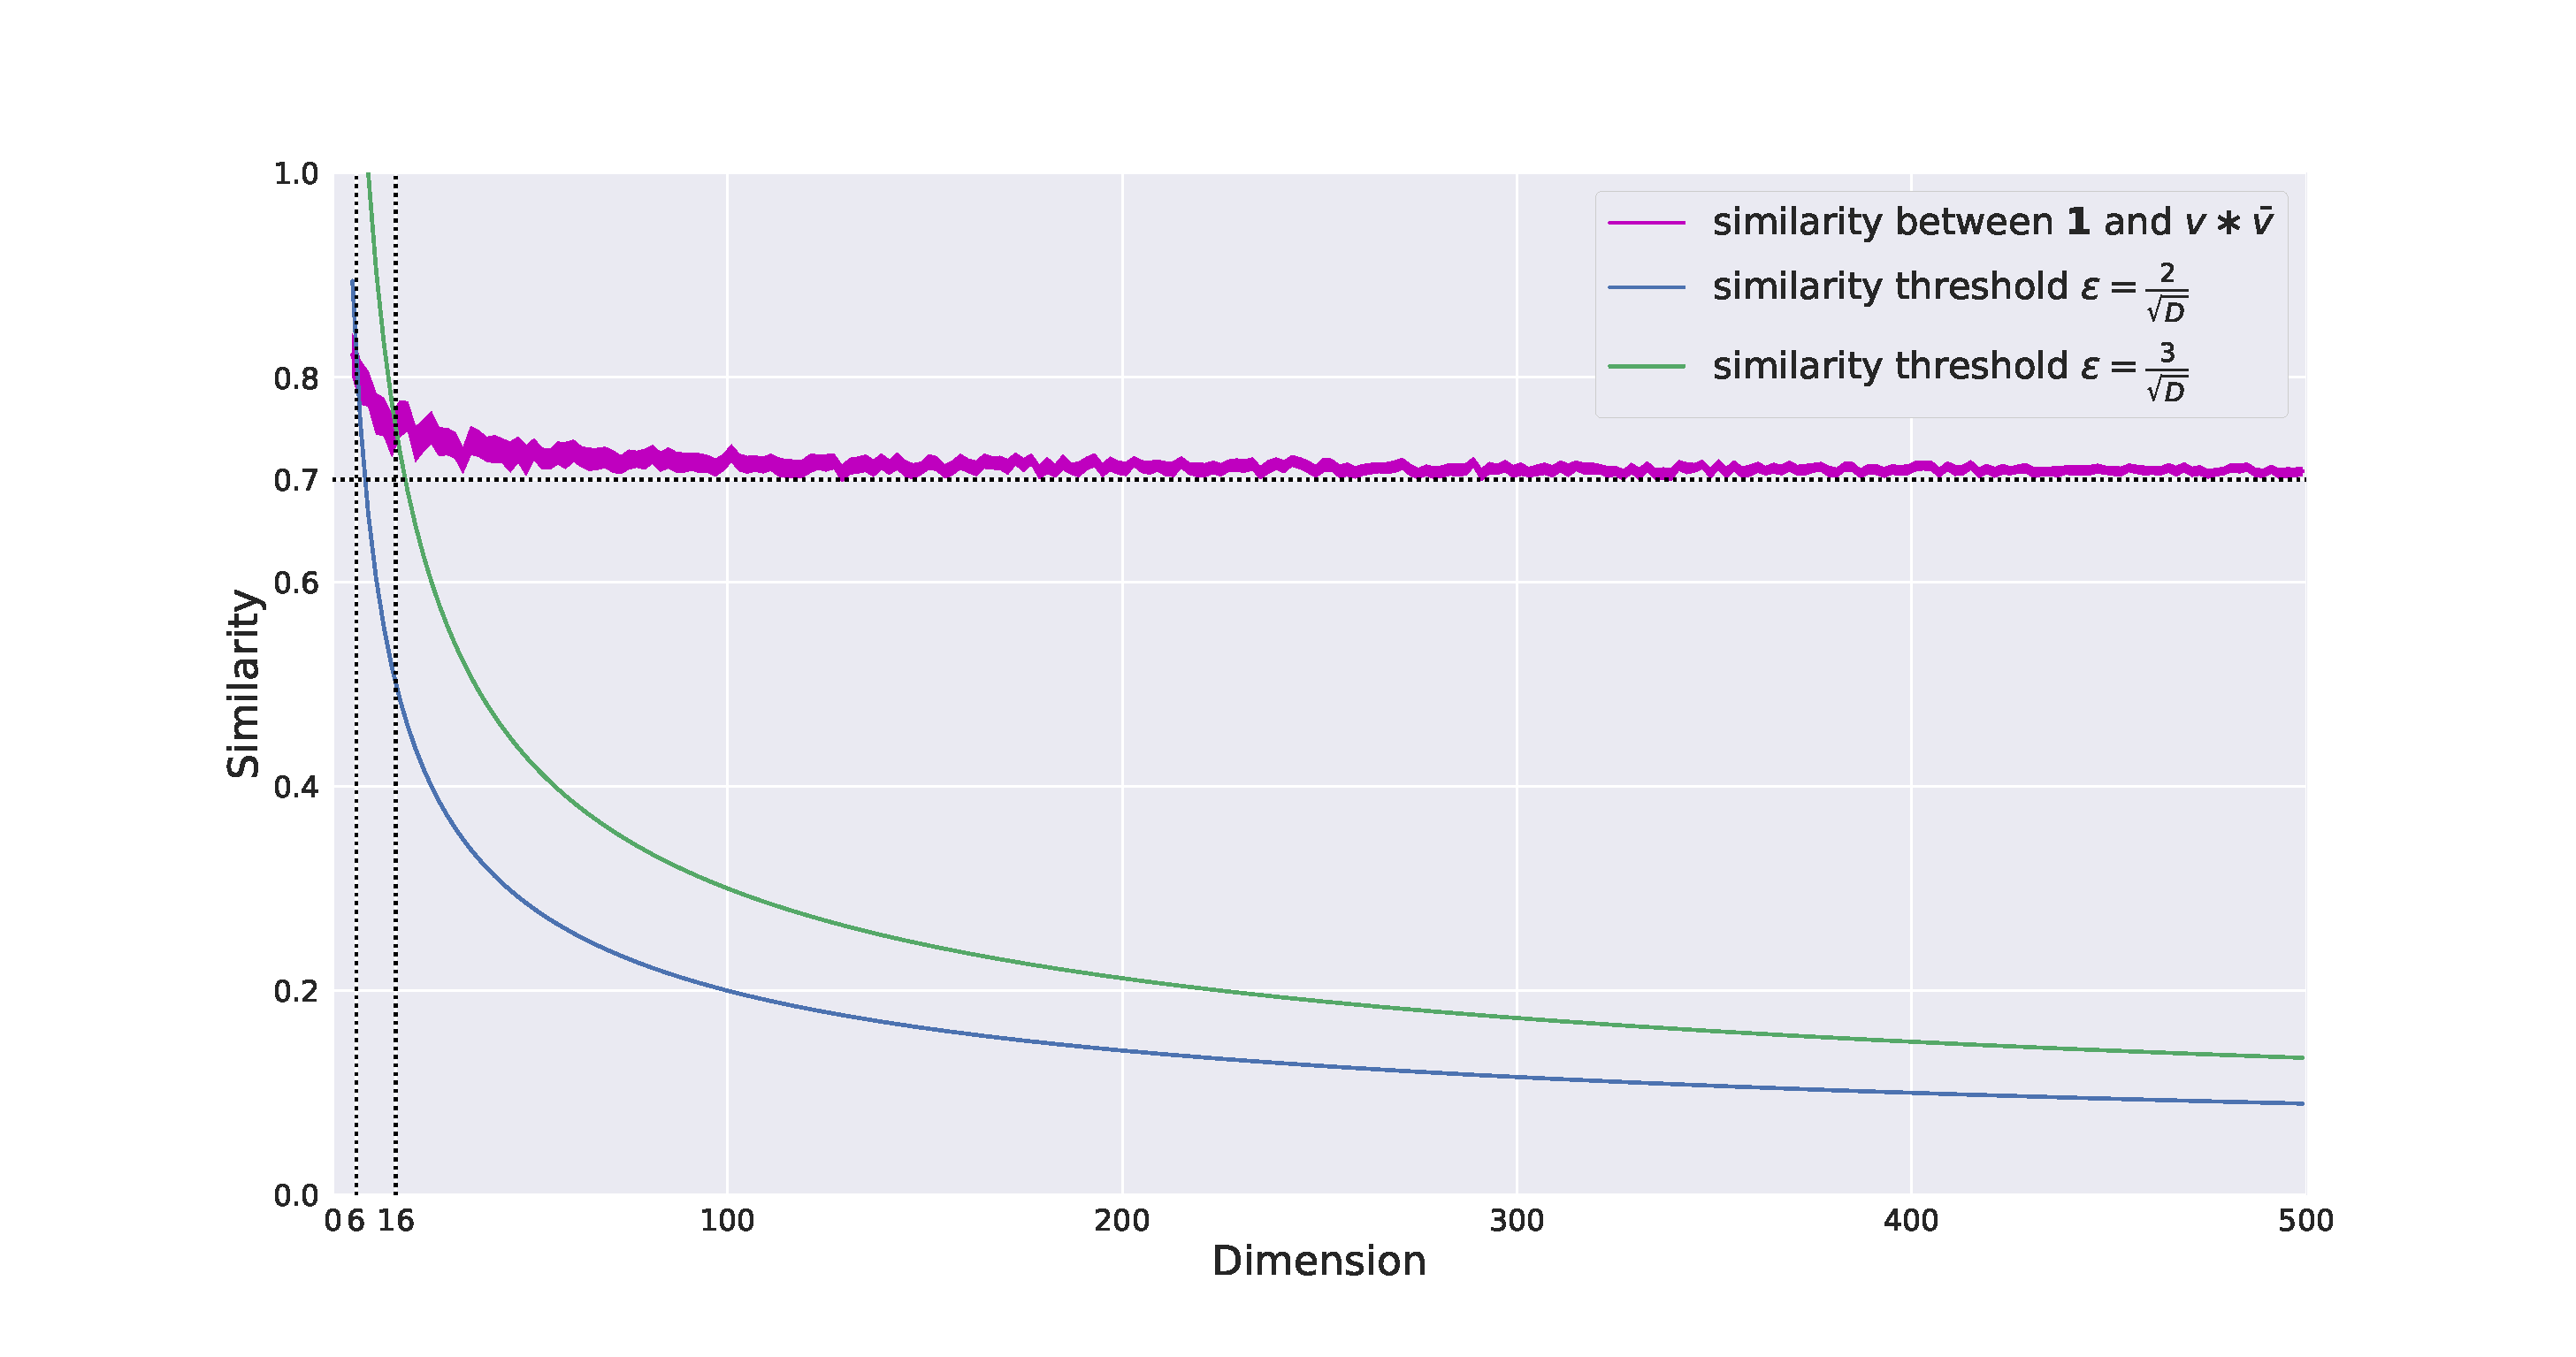
\includegraphics[width=1.0\textwidth]{imgs/pseudo_inverse_tsplot.eps}
	\caption{Visualization of the similarity $\phi\left(\mathbf{1}, v \varoast \bar{v}\right)$ between the neutral element $\mathbf{1}$ and the result of applying the pseudo-inverse to different vectors for varying vector dimensions. This plot shows the result of $100$ samples compared to the similarity threshold $\epsilon$.}
	\label{fig:pseudo_inv}
\end{figure}
\begin{lemma}
	\label{lemma:spa_pseudo_inv}
	Let $ \mathbf{v}=\left(v_0, \ldots, v_{D-1}\right)$ be an element of a $D$-dimensional \ac{SPA} $\mathcal{S}(D)$, i.e., $v_0, \ldots, v_{D-1} \in \mathbb{R}$.
	The vector $\bar{\mathbf{v}}=\left(v_0, v_{D-1}, \ldots, v_{1}\right)$ is a pseudo-inverse element of $ \mathbf{v}$ with respect to circular convolution, i.e., $ \mathbf{v} \varoast \bar{\mathbf{v}} \approx \mathbf{1}$.
\end{lemma}
Here, we skip an explicit proof for this lemma but rather point to \textcite[Section 3.1.2 and 3.1.3]{Plate1994} for a in-depth derivation.
However, we visualize the similarity $\phi\left(\mathbf{1}, \mathbf{v} \varoast \bar{\mathbf{v}}\right)$ between the neutral element $\mathbf{1}$ and the result of applying the pseudo-inverse $ \mathbf{v} \varoast \bar{\mathbf{v}}$ compared to the similarity threshold $\epsilon$ (weak and strong version) in Fig.~\ref{fig:pseudo_inv}.
Therefore, we randomly chose \num{100} sample vectors for various dimensions, convolved them with their pseudo-inverse and compared the result to the neutral element $\mathbf{1}$.
We observe, that this similarity remains almost constant slightly above \num{0.7} and already for low vector dimensions ($D > 20$) way above the strong similarity threshold of $\epsilon=\frac{3}{\sqrt{D}}$.

Lemma~\ref{lemma:spa_pseudo_inv} states that we can find a pseudo-inverse element $\bar{\mathbf{v}}$ for any vector $ \mathbf{v}$ in a $D$-dimensional \ac{SPA} (given the dimension $D$ is sufficiently large).
Although we can also find an exact inverse element $ \mathbf{v}^{-1}$ for most vectors $ \mathbf{v}$, it is often more useful to work with pseudo-inverses instead of exact inverse elements.
We have already seen, that we can use the \acf{DFT} and \acf{IDFT} to calculate circular convolution efficiently by element-wise multiplication  \parencite[this follows from the convolution theorem, see][Chap. 6]{Bracewell2000} in the frequency domain, i.e.,
\begin{equation}
    \mathbf{v} \varoast \mathbf{w} = \ac{IDFT}\left(\ac{DFT}( \mathbf{v}) \odot \ac{DFT}( \mathbf{w}) \right). \tag{\ref{eq:conv_with_dft} revisited}
\end{equation}
Furthermore, the \ac{DFT} of the convolutive neutral element $\mathbf{1} = \left(1, 0, \ldots, 0\right)$ is
\begin{equation}
	\ac{DFT}(\mathbf{1}) = \left(\exp\left(i0\right), \ldots, \exp\left(i0\right)\right) = \left(1, 1, \ldots, 1\right).
\end{equation}
This gives us a way of finding an exact inverse element $ \mathbf{v}^{-1}$ by
\begin{equation}
	\ac{DFT}(\mathbf{1}) = \ac{DFT}( \mathbf{v}) \odot \ac{DFT}( \mathbf{v}^{-1}).
\end{equation}
By denoting the $j$-th element of the Fourier Vector $\ac{DFT}( \mathbf{v})$ with $\ac{DFT}_{j}( \mathbf{v})$, we get
\begin{equation}
\label{eq:inv_elemtwise_fourier}
	\ac{DFT}_{j}( \mathbf{v}) \odot \ac{DFT}_{j}( \mathbf{v}^{-1}) = 1 \quad \textrm{ for } j \in \left\{0, \ldots, D-1\right\}.
\end{equation}
If we express $\ac{DFT}_{j}( \mathbf{v}) \in \mathbb{C}$ in polar coordinates, i.e., $\ac{DFT}_{j}( \mathbf{v}) = r_j \exp\left(i\varphi_j\right)$, we directly get from equation~\eqref{eq:inv_elemtwise_fourier} that $\ac{DFT}_{j}( \mathbf{v}^{-1}) = \frac{1}{r_j} \exp\left(-i\varphi_j\right)$.
By using the symmetry property of the real-valued \ac{DFT}, we can see that the transform $\ac{DFT}_j(\bar{\mathbf{v}})$ of the pseudo-inverse element $\bar{\mathbf{v}}$ from Lemma~\ref{lemma:spa_pseudo_inv} is the complex conjugate of $\ac{DFT}_j( \mathbf{v})$, i.e., we can write $\ac{DFT}_j(\bar{\mathbf{v}}) = r_j \exp\left(-i\varphi\right)$ in polar coordinates.
From those equations, we can see that the pseudo-inverse $\bar{\mathbf{v}}$ has the same norm as the original vector $ \mathbf{v}$, i.e., $\norm{ \mathbf{v}} = \norm{\bar{\mathbf{v}}}$, whereas the norm of the exact inverse $ \mathbf{v}^{-1}$ can become significantly larger than the norm of $ \mathbf{v}$ in some cases.
This is due to the fact that elements of the transform of the pseudo-inverse have the same lengths $r_j$ as the original vector, whereas the transformed elements of the exact inverse have lengths $\frac{1}{r_j}$, which can become significantly large when $r_j$ is close to $0$.
The relation between the vector norm and the magnitudes in the frequency domain is given by Parseval's theorem  \parencite[also known as Rayleigh's theorem, see][Chap. 6]{Bracewell2000}, which states
\begin{equation}
\label{eq:parseval}
\norm{\mathbf{v}}^2 = \sum_{k=0}^{D-1} \left| v_{k} \right|^{2} = \frac{1}{D} \sum_{k=0}^{D-1} \left|\ac{DFT}_{k}\left( \mathbf{v}\right)\right|^{2} = \sum_{k=0}^{D-1} r_{k}^{2}.
\end{equation}
This can lead to additional noise when retrieving vectors from structured representations (cf.\ equation~\eqref{eq:retrieval}).
However, there is a certain class of vectors, for which the pseudo- and exact inverse element coincide.
\begin{defn}
	\label{def:unitary_vec}
	Let $ \mathbf{v}$ be a vector in a $D$-dimensional \ac{SPA} $\mathcal{S}(D)$ with exact and pseudo-inverse elements $ \mathbf{v}^{-1}$ and $\bar{\mathbf{v}}$ respectively.
	We call $ \mathbf{v}$ a \emph{unitary vector}, if and only if $ \mathbf{v}^{-1} = \bar{\mathbf{v}}$.
	We denote the set of unitary vectors by $\mathcal{U} \subset \mathcal{S}(D)$.
\end{defn}
\begin{defn}
	\label{def:conv_power}
	Let $ \mathbf{v}$ be a vector in a $D$-dimensional \ac{SPA} $\mathcal{S}(D)$. We define the \emph{convolutive power} by an exponent $p \in \mathbb{R}$ by
	\[
	\mathbf{v}^{p} := \Re\left(\ac{IDFT} \left(\left(\ac{DFT}_{j}\left( \mathbf{v}\right)^{p}\right)_{j=0}^{D-1}\right)\right),
	\]
	where $\Re$ denotes the real part $a$ of a complex number $a + ib \in \mathbb{C}$.
\end{defn}
Unitary vectors take a special role in the \ac{SPA} as they have some interesting and useful properties.
\begin{lemma}
	\label{lemma:unitary_vec}
	Let $\mathcal{U}$ be the set of unitary vectors in the $D$-dimensional \ac{SPA} $\mathcal{S}(D)$.
    The following statements hold
 	\begin{enumerate}[label=\roman*]
		\item All elements of $\mathcal{U}$ have unit length, i.e., we have $\norm{\mathbf{u}} = 1$ for any vector $ \mathbf{u} \in \mathcal{U}$.
		\item $\mathcal{U}$ is closed under convolutive exponentiation, i.e., $ \mathbf{u}^{p} \in \mathcal{U}$ for any $ \mathbf{u} \in \mathcal{U}$ and $p \in \mathbb{R}$.
        \item The product under circular convolution of two unitary vectors is unitary, i.e.\ $ \mathbf{u}_{1} \varoast \mathbf{u}_{2} \in \mathcal{U} $ for $ \mathbf{u}_{1}, \mathbf{u}_{2} \in \mathcal{U}.$
		\item Convolution with unitary vectors preserves the norm, i.e., $\norm{\mathbf{v}} = \norm{ \mathbf{v} \varoast \mathbf{u}}$ for any $ \mathbf{v} \in \mathcal{S}(D), \mathbf{u} \in \mathcal{U}$.
	\end{enumerate}
\end{lemma}
\begin{proof}
	To show that unitary vectors have unit length, we directly calculate the first component of convolution $ \mathbf{z} := \mathbf{u} \varoast \bar{ \mathbf{u}}$ between a unitary vector $ \mathbf{u}$ and its pseudo-inverse $\bar{ \mathbf{u}}$:
	\[
	z_{0} = \sum_{k=0}^{D-1} u_{k} \bar{u}_{-k \Mod{D}} = \sum_{k=0}^{D-1} u_{k}^{2} = \norm{ \mathbf{u}}^{2}.
	\]
	Since $ \mathbf{u}$ is a unitary vector, we have $ \mathbf{u}^{-1} = \bar{ \mathbf{u}}$ and therefore $ \mathbf{u}\varoast \bar{ \mathbf{u}} = \mathbf{1}$.
	Thus, for the first component of $ \mathbf{z} := \mathbf{u} \varoast \bar{ \mathbf{u}}$, we have 
	\[
	1 = z_{0} = \norm{ \mathbf{u}}^{2},
	\]
	which gives the first result of the lemma.
    
	To show that the set of unitary vectors $\mathcal{U}$ is closed under convolutive exponentiation, we write each component of $\ac{DFT}( \mathbf{u})$ for $ \mathbf{u} \in \mathcal{U}$ in polar coordinates, i.e., $\ac{DFT}_j( \mathbf{u}) = r_j\exp\left(\varphi_j\right)$.
	From previous considerations, we know that $\ac{DFT}_j( \mathbf{u}^{-1}) = \frac{1}{r_j}\exp\left(-\varphi_j\right)$ and $\ac{DFT}_j(\bar{ \mathbf{u}}) = r_j\exp\left(-\varphi_j\right)$, which gives $r_j=1$ for $j=0, \ldots, D-1$ because $ \mathbf{u}$ is a unitary vector.
	Thus, for any $p \in \mathbb{R}$, we have 
	\[
	\ac{DFT}_j\left( \mathbf{u}^{p}\right) = \ac{DFT}_j\left( \mathbf{u}\right)^{p} = r_j^{p}\exp\left(ip\varphi\right) = 1^{p} \cdot \exp\left(ip\varphi\right),
	\]
	which makes $ \mathbf{u}^{p}$ itself a unitary vector, as all magnitudes are $1$.	

    Similarly, we proof that the convolution of two unitary vectors is again unitary. 
    Let $ \mathbf{u}_{1}, \mathbf{u}_{2} \in \mathcal{U}$ be unitary vectors, then we have
    \[
        \ac{DFT} \left( \mathbf{u}_1 \varoast \mathbf{u}_2\right) = \ac{DFT} \left( \ac{IDFT} \left( \ac{DFT} \left( \mathbf{u}_1\right) \odot \ac{DFT} \left( \mathbf{u}_2\right)\right)\right) =  \ac{DFT} \left( \mathbf{u}_1\right) \odot \ac{DFT} \left( \mathbf{u}_2\right).
    \]
    Writing both $\ac{DFT}_j( \mathbf{u}_1) = r_{1j}\exp\left(\varphi_{1j}\right)$ and $\ac{DFT}_j( \mathbf{u}_2) = r_{2j}\exp\left(\varphi_{2j}\right)$ in polar coordinates, we get 
    \[
        \ac{DFT}_j \left( \mathbf{u}_1 \varoast \mathbf{u}_2\right) = r_{1j} \cdot r_{2j} \cdot \exp \left(\varphi_{1j} + \varphi_{2j}\right) = 1 \cdot \exp \left(\varphi_{1j} + \varphi_{2j}\right),
    \]
    as we have $r_{1j}=1$ and $r_{2j}=1$ for all magnitudes since both $ \mathbf{u}_1$ and $ \mathbf{u}_2$ are unitary vectors.
    This in turn makes their product under convolution unitary as well.
    
    To proof that convolution with unitary vectors preserves the norm, we use Parseval's theorem (cf.\ equation~\eqref{eq:parseval}) again.
	For any vector $ \mathbf{v} \in \mathcal{S}(d)$ and  a unitary vector $ \mathbf{u} \in \mathcal{U}$, we denote $ \mathbf{z}:=  \mathbf{v} \varoast \mathbf{u}$ and get
	\begin{equation}
	\label{eq:norm_parseval}
	\norm{ \mathbf{v} \varoast \mathbf{u}}^{2} = \sum_{k=0}^{D-1} \left|z_{k}\right|^{2} = \frac{1}{D} \sum_{k=0}^{D-1} \left|\ac{DFT}_{k}( \mathbf{z})\right|^{2} = \frac{1}{D} \sum_{k=0}^{D-1} \left|\ac{DFT}_{k}( \mathbf{v}) \cdot \ac{DFT}_{k}( \mathbf{u})\right|^{2}.
	\end{equation}
	Writing $\ac{DFT}_{k}( \mathbf{v}) = r_{vk}\exp\left(i\varphi_{vk}\right)$ and $\ac{DFT}_{k}( \mathbf{u}) = r_{uk}\exp\left(i\varphi_{uk}\right)$ in polar coordinates, with $r_{uk} = 1$ for $k=0, \ldots, D-1$ as $ \mathbf{u}$ is unitary, equation~\eqref{eq:norm_parseval} transforms to
	\begin{equation*}
	\norm{ \mathbf{v} \varoast \mathbf{u}}^{2} = \frac{1}{D} \sum_{k=0}^{D-1} \left|r_{vk} \exp\left(i\left(\varphi_{vk} + \varphi_{uk}\right)\right)\right|^{2} = \frac{1}{D} \sum_{k=0}^{D-1} \left|r_{vk}\right|^{2} = \frac{1}{D} \sum_{k=0}^{D-1} \left|\ac{DFT}_k\left( \mathbf{v}\right)\right|^{2} = \norm{ \mathbf{v}}^{2}.
	\end{equation*}
\end{proof}

%----------------------------------------------------------------------------------------------------------
\section{The \acl{NEF}}
\label{sec:neural_eng}
%----------------------------------------------------------------------------------------------------------

In this section, we make a short excursion and give a brief overview of the \acf{NEF}, as we will be making use of it in forthcoming chapters.
The \ac{NEF} \parencite{Eliasmith2003} is a mathematical theory, which provides a set of methods to construct biologically plausible, large-scale neural models.
These methods can be divided into the three main principles of the \ac{NEF}: \emph{representation}, \emph{transformation} and \emph{dynamics}.
The \ac{Nengo} \footfullcite{Nengo} software suite is a python library, which implements the \ac{NEF}'s principles \parencite{Bekolay2014}.
\ac{Nengo} has been used to build a variety of neural models, e.g., models of the Basal Ganglia system \parencite{Stewart2010, Stewart2012} and \acf{Spaun}, a large-scale, functional model of the brain, which is able to perform eight cognitive tasks \parencite{Eliasmith2012}.
Furthermore, \ac{Nengo} has been used to interface neural models with physical, neuromorphic hardware systems and robots \parencites{Conradt2014, Stewart2016}.
Here, we give a brief introduction to the \ac{NEF}'s principles and refer to \textcite{Eliasmith2003, Eliasmith2013, Bekolay2014} for more details.
\subsection{Representation}
\label{subsec:nef_representation}
The first principle of the \ac{NEF}, representation, provides mathematical tools to encode information, namely time-varying real-valued vectors, in the activity of neural populations.
It is based on the assumption, that neurons have a \enquote{preferred direction vector} in the represented space, each neuron responds most strongly to.
This assumption is grounded by the findings of \textcite{Georgopoulos1989} that each neuron in motor cortex of rhesus monkeys has a different preferred arm direction.
The \ac{NEF} expands this idea to neural representations in general.
\begin{figure}[t!]
	\centering
	\subfloat[Tuning curves \label{subfig:nef_rep_tuning_curves}]{%
		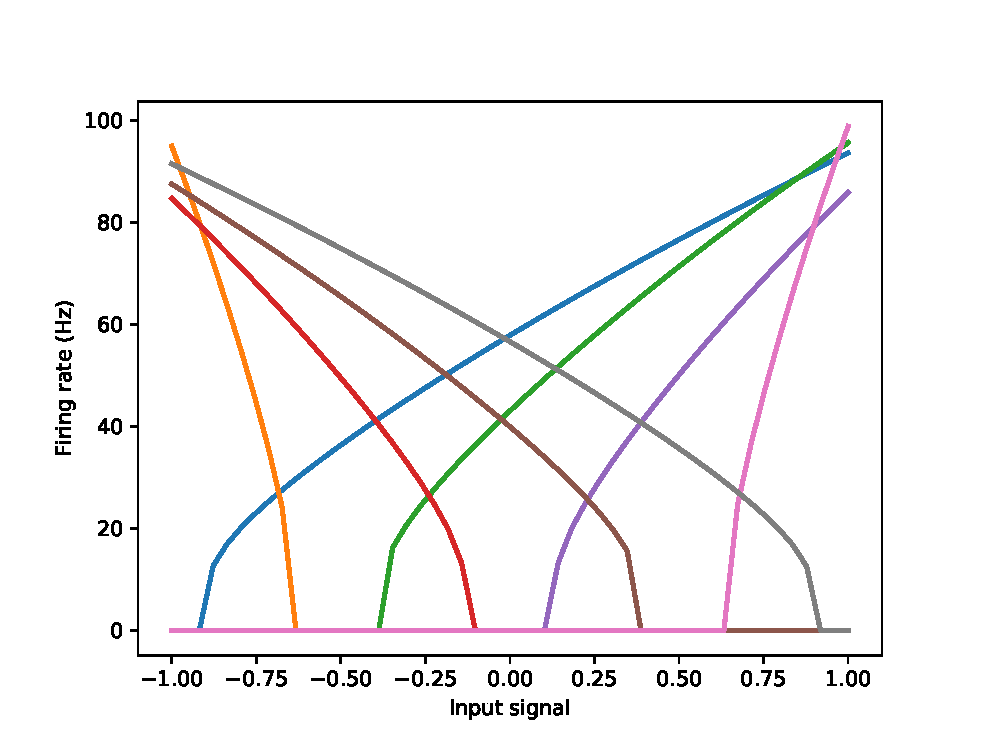
\includegraphics[width=0.45\textwidth]{imgs/NEF_tuning_curves.eps}
	}
	\subfloat[Spike times\label{subfig:nef_rep_spike_raster}]{%
		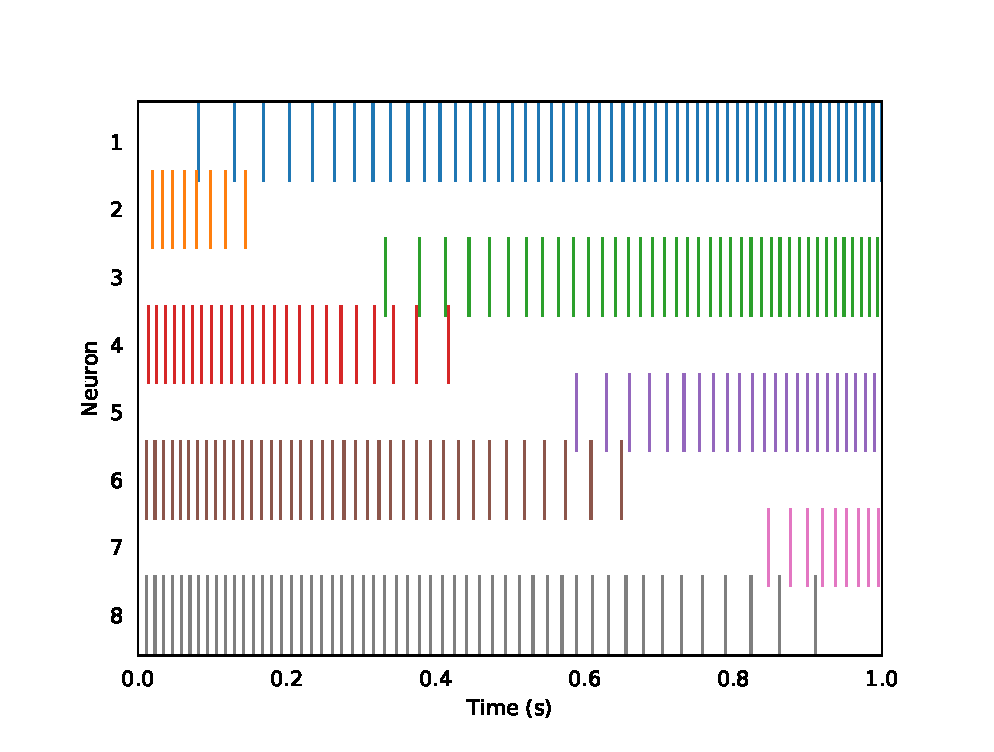
\includegraphics[width=0.45\textwidth]{imgs/NEF_spikes_raster.eps}
	}\\
	\vspace{-0.4cm}
	\subfloat[Decoded output\label{subfig:nef_rep_decoded}]{%
		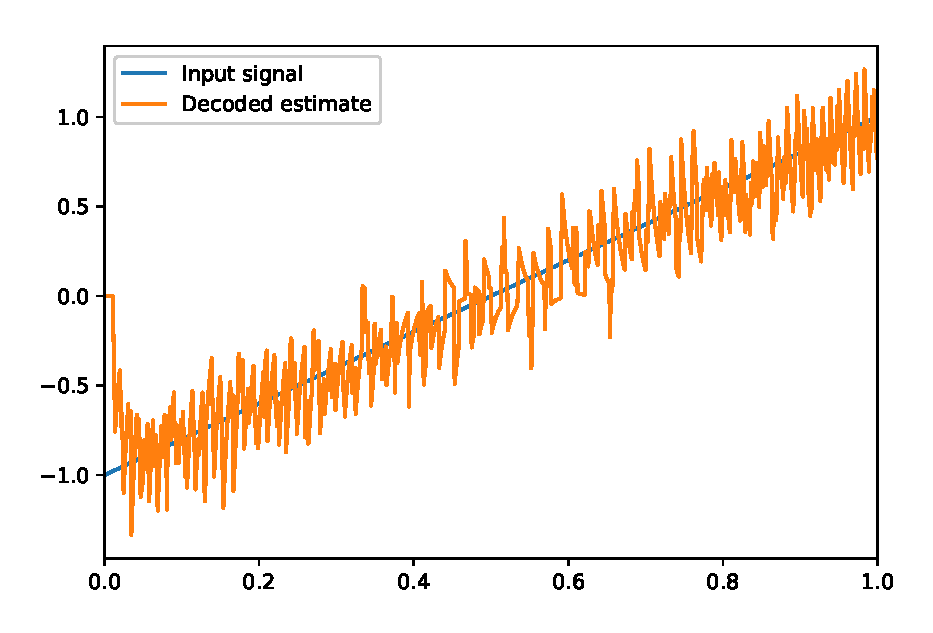
\includegraphics[width=0.45\textwidth]{imgs/NEF_decoded_output.eps}
	}
	\subfloat[Filtered neural activity\label{subfig:nef_rep_spike_filtered}]{%
		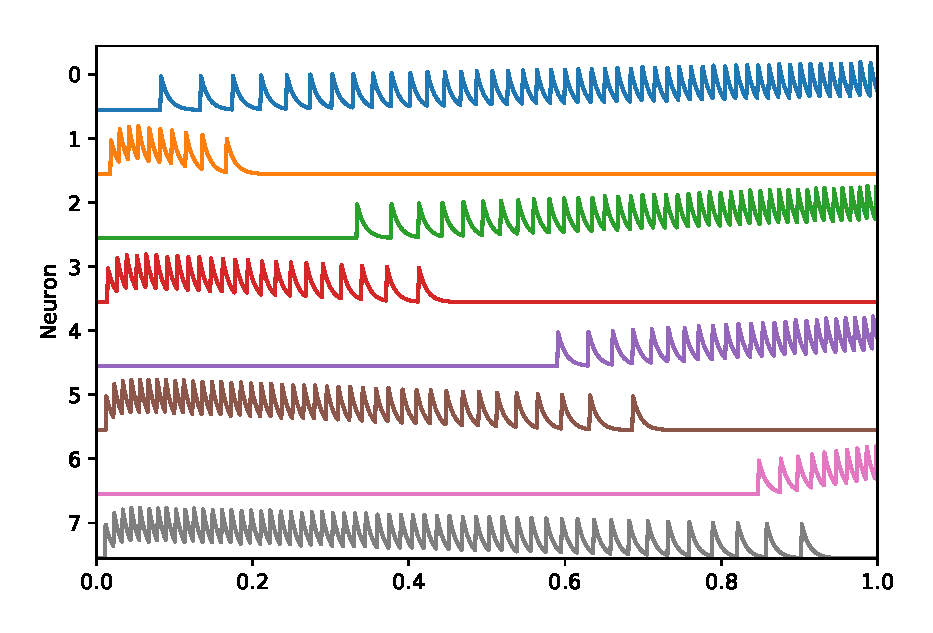
\includegraphics[width=0.45\textwidth]{imgs/NEF_spikes_filtered.eps}
	}
	\caption{The representation principle of the \ac{NEF}. 
    Images adapted from \textcite{Bekolay2014}.}
    \label{fig:nef_representation}
\end{figure}
Let $A$ be a population of $N \in \mathbb{N}$ neurons encoding a subset $V$ of a real-valued vector space, i.e., $V\subseteq \mathbb{R}^{n}$.
Given a function $\abbil{\mathbf{x}}{\mathbb{R}}{V}$, we can write the activity $a_{i}$ of the $i$-th neuron in a neural population encoding a time-varying vector $\mathbf{x}(t)$ as a spike train, i.e., a sum of delta functions
\begin{equation}
a_{i}\left(\mathbf{x}(t)\right) = \sum_{j=1}^{m_{i}} \delta(t - t_{j}) = G_{i}(\underbrace{\alpha_{i}\langle\mathbf{e}_{i},\mathbf{x}(t)\rangle + J_{i}}_{=:c}) \quad \textrm{ for } 1 \leq i \leq N,
\label{eq:nef_encoding}
\end{equation}
where $G_{i}$ is the spiking neural non-linearity, $\alpha_{i}$ is the gain of the neuron, $\mathbf{e}_{i}$ is the neuron's preferred direction or encoding vector and $J_{i}$ is a bias current to account for neural background activity and $t_{j}$ are the $m_{i}$ spike-times of the $i$-th neuron.
Notably, the current flowing into the cell is completely determined by $c$, whereas the spiking behavior of the neuron model is represented by the non-linear function $G_{i}$.
The input current $c$ and therefore the \ac{NEF}'s encoding process is independent of particular spiking neuron models.

To decode the input values $\mathbf{x}(t)$ back out of the neural population $A$, the spike train is convolved with an exponentially decaying filter $\abbil{h}{\mathbb{R}}{\mathbb{R}}$ to simulate the process of neurons generating post-synaptic current after spiking (cf.\ Fig.~\ref{subfig:nef_rep_spike_filtered}) resulting in
\begin{equation}
\tilde{a}_{i}\left(\mathbf{x}(t)\right) = \sum_{j=1}^{m_{i}} h(t) \ast \delta(t - t_{j}) = \sum_{j=1}^{m_{i}} h(t - t_{j}).
\label{eq:nef_filtered_activity}
\end{equation}
A simple model of an exponential decaying filter is the function $\abb{h}{\mathbb{R}}{\mathbb{R}}{t}{e^{\sfrac{-t}{\tau_{p}}}}$, where $\tau_{P}$ denotes the post-synaptic time constant.
We obtain an estimation $\mathbf{\hat{x}}(t)$ of the original input $\mathbf{x}(t)$ as a weighted sum with some decoder values $\mathbf{d}_{i}$
\begin{equation}
\mathbf{\hat{x}}(t) = \sum_{i=1}^{N} \tilde{a}_{i}\left(\mathbf{x}(t)\right) \mathbf{d}_{i}.
\label{eq:nef_decoding}
\end{equation}
To calculate the optimal decoders $\mathbf{d}_{i}$, we need to minimize the error between input $\mathbf{x}(t)$ and decoded output $\mathbf{\hat{x}}(t)$
\begin{equation}
E = \int \left( \mathbf{x}(t) - \sum_{i=1}^{N} \tilde{a}_{i}\left(\mathbf{x}(t)\right) \mathbf{d}_{i}\right)^{2} \diff \mathbf{x}(t).
\label{eq:decoder_calculation}
\end{equation}
\ac{Nengo} solves for the decoders $\mathbf{d}_{i}$ by default using least squares optimization \parencite{Eliasmith2013}[Appendix B1].
Figure~\ref{fig:nef_representation} visualizes this encoding process for $V = \left[ -1, 1\right] \subset \mathbb{R}$ and a population of $8$ neurons.
Figure~\ref{subfig:nef_rep_tuning_curves} shows the tuning curves of individual neurons, which define how these neurons respond to specific input values.
Equation~\eqref{eq:nef_encoding} is depicted in Fig.~\ref{subfig:nef_rep_spike_raster}, which shows a raster plot of the neurons' spike times based on the input signal shown in Fig.~\ref{subfig:nef_rep_decoded}.
Figure~\ref{subfig:nef_rep_spike_filtered}, which shows the filtered neural activity for each neuron, visualizes Equation~\eqref{eq:nef_filtered_activity}.
Finally, Fig.~\ref{subfig:nef_rep_decoded} depicts the original input value as well as the estimated output of the neural populations' activity (cf.\ Equation~\eqref{eq:nef_decoding}).
Note, that the neural population's decoded output is only a noisy approximation of the original input value, whose accuracy can be improved by increasing the number of neurons in the population.
\subsection{Transformation}
\begin{figure}[t]
	\centering
	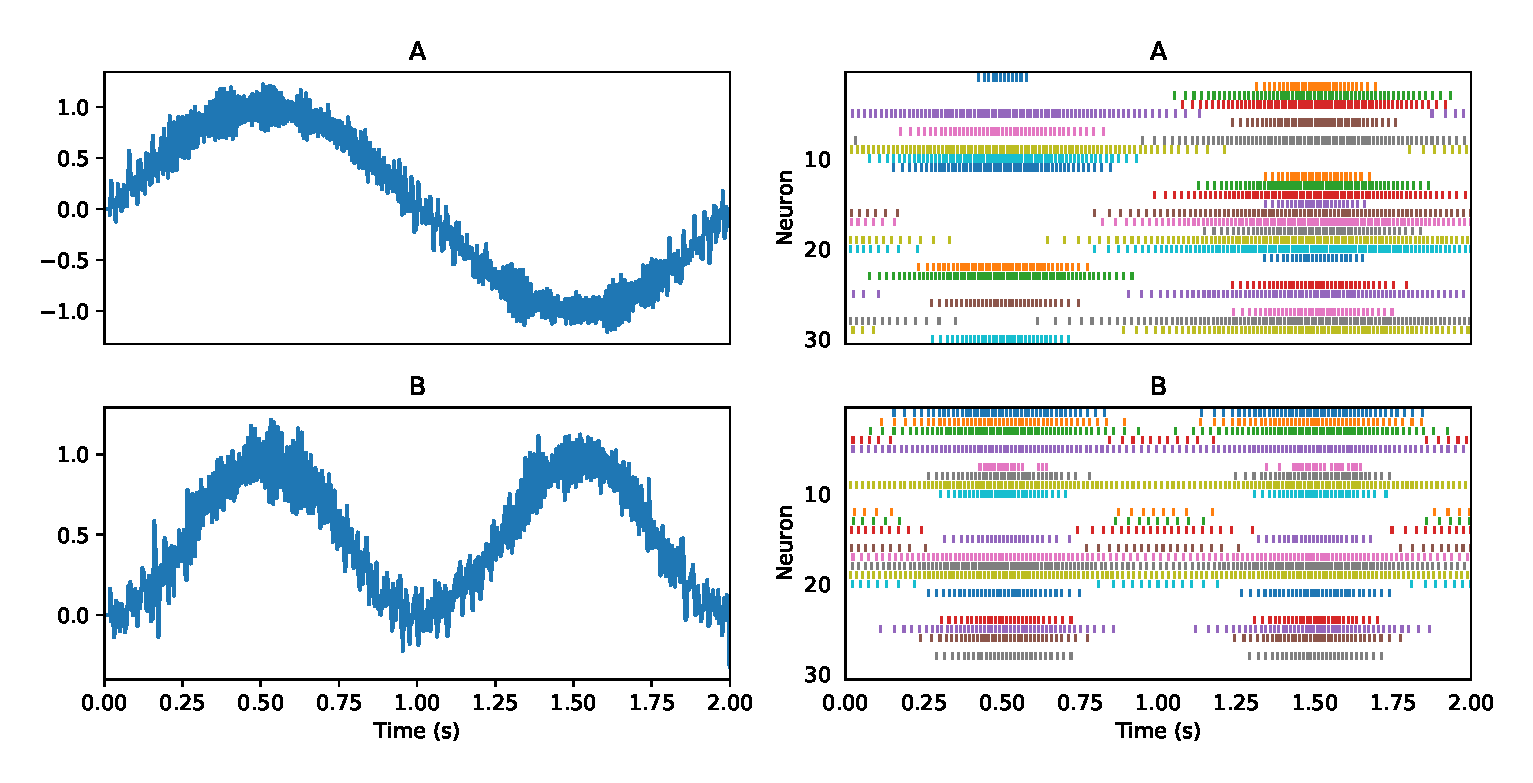
\includegraphics[width=0.95\textwidth]{imgs/NEF_transformation.eps}
	\caption{The transformation principle of the \ac{NEF}.
    Images adapted from \textcite{Nengo}.}
	\label{fig:nef_transformation}
\end{figure}
The second main principle of the \ac{NEF}, \emph{transformation}, provides the mathematical tools to compute functions across connections between populations of neurons.
Let $A$ resp. $B$ be populations of $N$ resp. $M$ neurons encoding a time-varying vector $\mathbf{x}(t) \in V \subset \mathbb{R}^{n}$ resp. $\mathbf{y}(t) \in W \subset \mathbb{R}^{m}$ according to the representation principle and a function $\abbil{f}{V}{W \subset \mathbb{R}^{m}}$.
In order to approximate the function $f$ across a connection from population $A$ to population $B$, we use the tools of the representation principle, but we calculate a different set of decoder values $\mathbf{d}_{i}^{f}$ for population $A$ by minimizing the error
\begin{equation}
\label{eq:nef_transformation}
E = \int \left( f(\mathbf{x}(t)) - \sum_{i=1}^{N} \tilde{a}_{i}\left(\mathbf{x}(t)\right) \mathbf{d}_{i}^{f}\right)^{2} \diff \mathbf{x}(t).
\end{equation}
Given encoders $\mathbf{e}_{j}^{B}$ and gain $\alpha_{j}^{B}$ for $1 \leq j \leq M$ of population $B$, we can derive a weight matrix for the connection from $A$ to $B$ approximating the function $f$ by
\begin{equation}
w_{ij} = \alpha_{j}^{B} \mathbf{d}_{i}^{f} L \mathbf{e}_{j}^{B} \quad \textrm{for } 1 \leq i \leq N \textrm{ and } 1 \leq j \leq M,
\end{equation}
where $L$ is a $M \times N$ linear operator.
Here, the \ac{NEF} makes the assumption, that connection weights can be factored into encoders, decoders and a linear transform.
Figure~\ref{fig:nef_transformation} visualizes the \ac{NEF}'s transformation principle for $V = W = \left[ -1, 1\right] \subset \mathbb{R}$, two neural populations $A$, $B$ containing $30$ neurons each.
The left panel of plots shows the populations' decoded outputs whereas the right panel depicts the neurons' spike times.
Population $A$ uses the representation principle to encode a sine function, whereas the transformation principle was used to calculate the function $\abb{f}{V}{W}{x}{f(x)=x^{2}}$ across the connection from $A$ to $B$.

\subsection{Dynamics}

\begin{figure}[t]
	\centering
\begin{tikzpicture}[%
auto,
%scale=3,
block/.style={
	rectangle,
	draw=blue,
	thick,
	fill=blue!20,
	text width=3em,
	align=center,
	rounded corners,
	minimum height=4em,
},
circ/.style={
	circle,
	draw=orange,
	thick,
	fill=orange!20,
	text width=3em,
	align=center,
	rounded corners,
	minimum height=6em,
}
]
\node[block] (X) at (1,1) {\Huge $\mathbf{x}$};
\node[circ] (A) [right=2cm of X] {\Huge  $A$ \\ \vspace{0.5em} \Large $\ast h(t)$};
\node[block] (Y) [right=2cm of A] {\Huge $\mathbf{y}$};
\draw [thick,->] (X) -- (A) node [midway, below] {\Large $f\left(\mathbf{x}\left(t\right)\right)$};
\draw [thick,->] (A) -- (Y);
% Calculate branch point coordinates
\path (A) -- coordinate (branch) (Y);
\path (X) -- coordinate (branch_end) (A);
\coordinate[above=2cm of branch] (branch_ab);
\coordinate[above=2cm of branch_end] (branch_end_ab);
\draw [thick,->] (branch) -- (branch_ab) -- (branch_end_ab) node [midway, above] {\Large $g\left(\mathbf{y}\left(t\right)\right)$} -- (branch_end);
\end{tikzpicture}
\caption{The dynamics principle of the \ac{NEF} for recurrent connections.}
\label{fig:nef_dynamics}
\end{figure}

%\todo[inline]{check if figure~\ref{fig:nef_dynamics} can be beautified}

The third main principle of the \ac{NEF}, \emph{dynamics}, provides a set of mathematical tools to implement dynamical systems in neural populations through recurrent connections.
Let $A$ be a population of neurons with an incoming connection approximating the function $\abbil{f}{V}{W \subset \mathbb{R}^{m}}$ and a recurrent connection approximating the function $\abbil{g}{W}{W}$ (cf.\ Fig.~\ref{fig:nef_dynamics}).
Thus, the overall function the population is approximating is
\begin{equation}
\mathbf{y}(t) = h(t) \ast \left(f(\mathbf{x}(t)) + g(\mathbf{y}(t))\right)
\label{eq:nef_dyn}
\end{equation}
with exponential decaying filter function $\abb{h}{\mathbb{R}}{\mathbb{R}}{t}{e^{\sfrac{-t}{\tau}}}$.
By applying the Laplace transform to Equation~\eqref{eq:nef_dyn}, we get
\begin{equation}
\label{eq:nef_dyn_laplace}
\mathbf{Y}(s) = \frac{1}{1 + s\tau}\left(F(\mathbf{X}(s)) + G(\mathbf{Y}(s))\right).
\end{equation}
We can rearrange Equation~\eqref{eq:nef_dyn_laplace} to
\begin{equation}
s\mathbf{Y}(s) = \frac{G(\mathbf{Y}(s))-\mathbf{Y}(s)}{\tau} + \frac{F(\mathbf{X}(s))}{\tau}.
\end{equation}
Transforming back leads to the differential equation
\begin{equation}
\frac{\partial \mathbf{y}(t)}{\partial t} = \frac{g(\mathbf{y}(t)-y)}{\tau} + \frac{f(\mathbf{x}(t))}{\tau}.
\end{equation}
Thus, to construct a neural model approximating a differential equation of the form
\begin{equation}
\frac{\partial \mathbf{y}(t)}{\partial t} = a(\mathbf{y}(t)) + b(\mathbf{x}(t))
\label{eq:nef_dyn_diffeq}
\end{equation}
with functions $\abbil{a}{W}{W}$ and $\abbil{b}{V}{W}$, the first two principles of the \ac{NEF} can be used to create a neural population of the form as shown in Fig.~\ref{fig:nef_dynamics}.
By setting the functions $g(\mathbf{y}(t))=\tau a(\mathbf{y}(t)) + \mathbf{y}(t)$ and $f(\mathbf{x}(t))=\tau b(\mathbf{x}(t))$, we obtain a neural model approximating the desired dynamical system described by the differential Equation~\eqref{eq:nef_dyn_diffeq}.

\section{Cognitive Modeling with \aclp{VSA}}%
\label{sec:cognitive_modelling_with_vsa}

In this section, we give a brief introduction of how we can use the theory shown in sections~\ref{sec:math_prop_vsas} and~\ref{sec:spa} to represent (structured) information using \acp{VSA}.
We give a general overview of different ways to establish vocabularies containing atomic vectors and how we can build more complex representations from those elementary ingredients.
\textcite{Gallant2013} refer to these two steps as the first two of three stages for generating structured vector representations: the \emph{pre-processing stage} (generating a vocabulary; see also section~\ref{sec:preprocessing_stage_generating_a_vocabulary}) and the \emph{representation generation stage} (building structured representations from the vocabulary; see also~\ref{sec:representation_generation_stage}).
Furthermore, we will see how these representations can be implemented in \acp{SNN} using the principles of the \ac{NEF} described in section~\ref{sec:neural_eng}.

\subsection{Vocabularies}
\label{subsec:vocabs}

\begin{figure}[t!]
	\centering
	\subfloat[\label{subfig:conceptual_golfball}]{%
		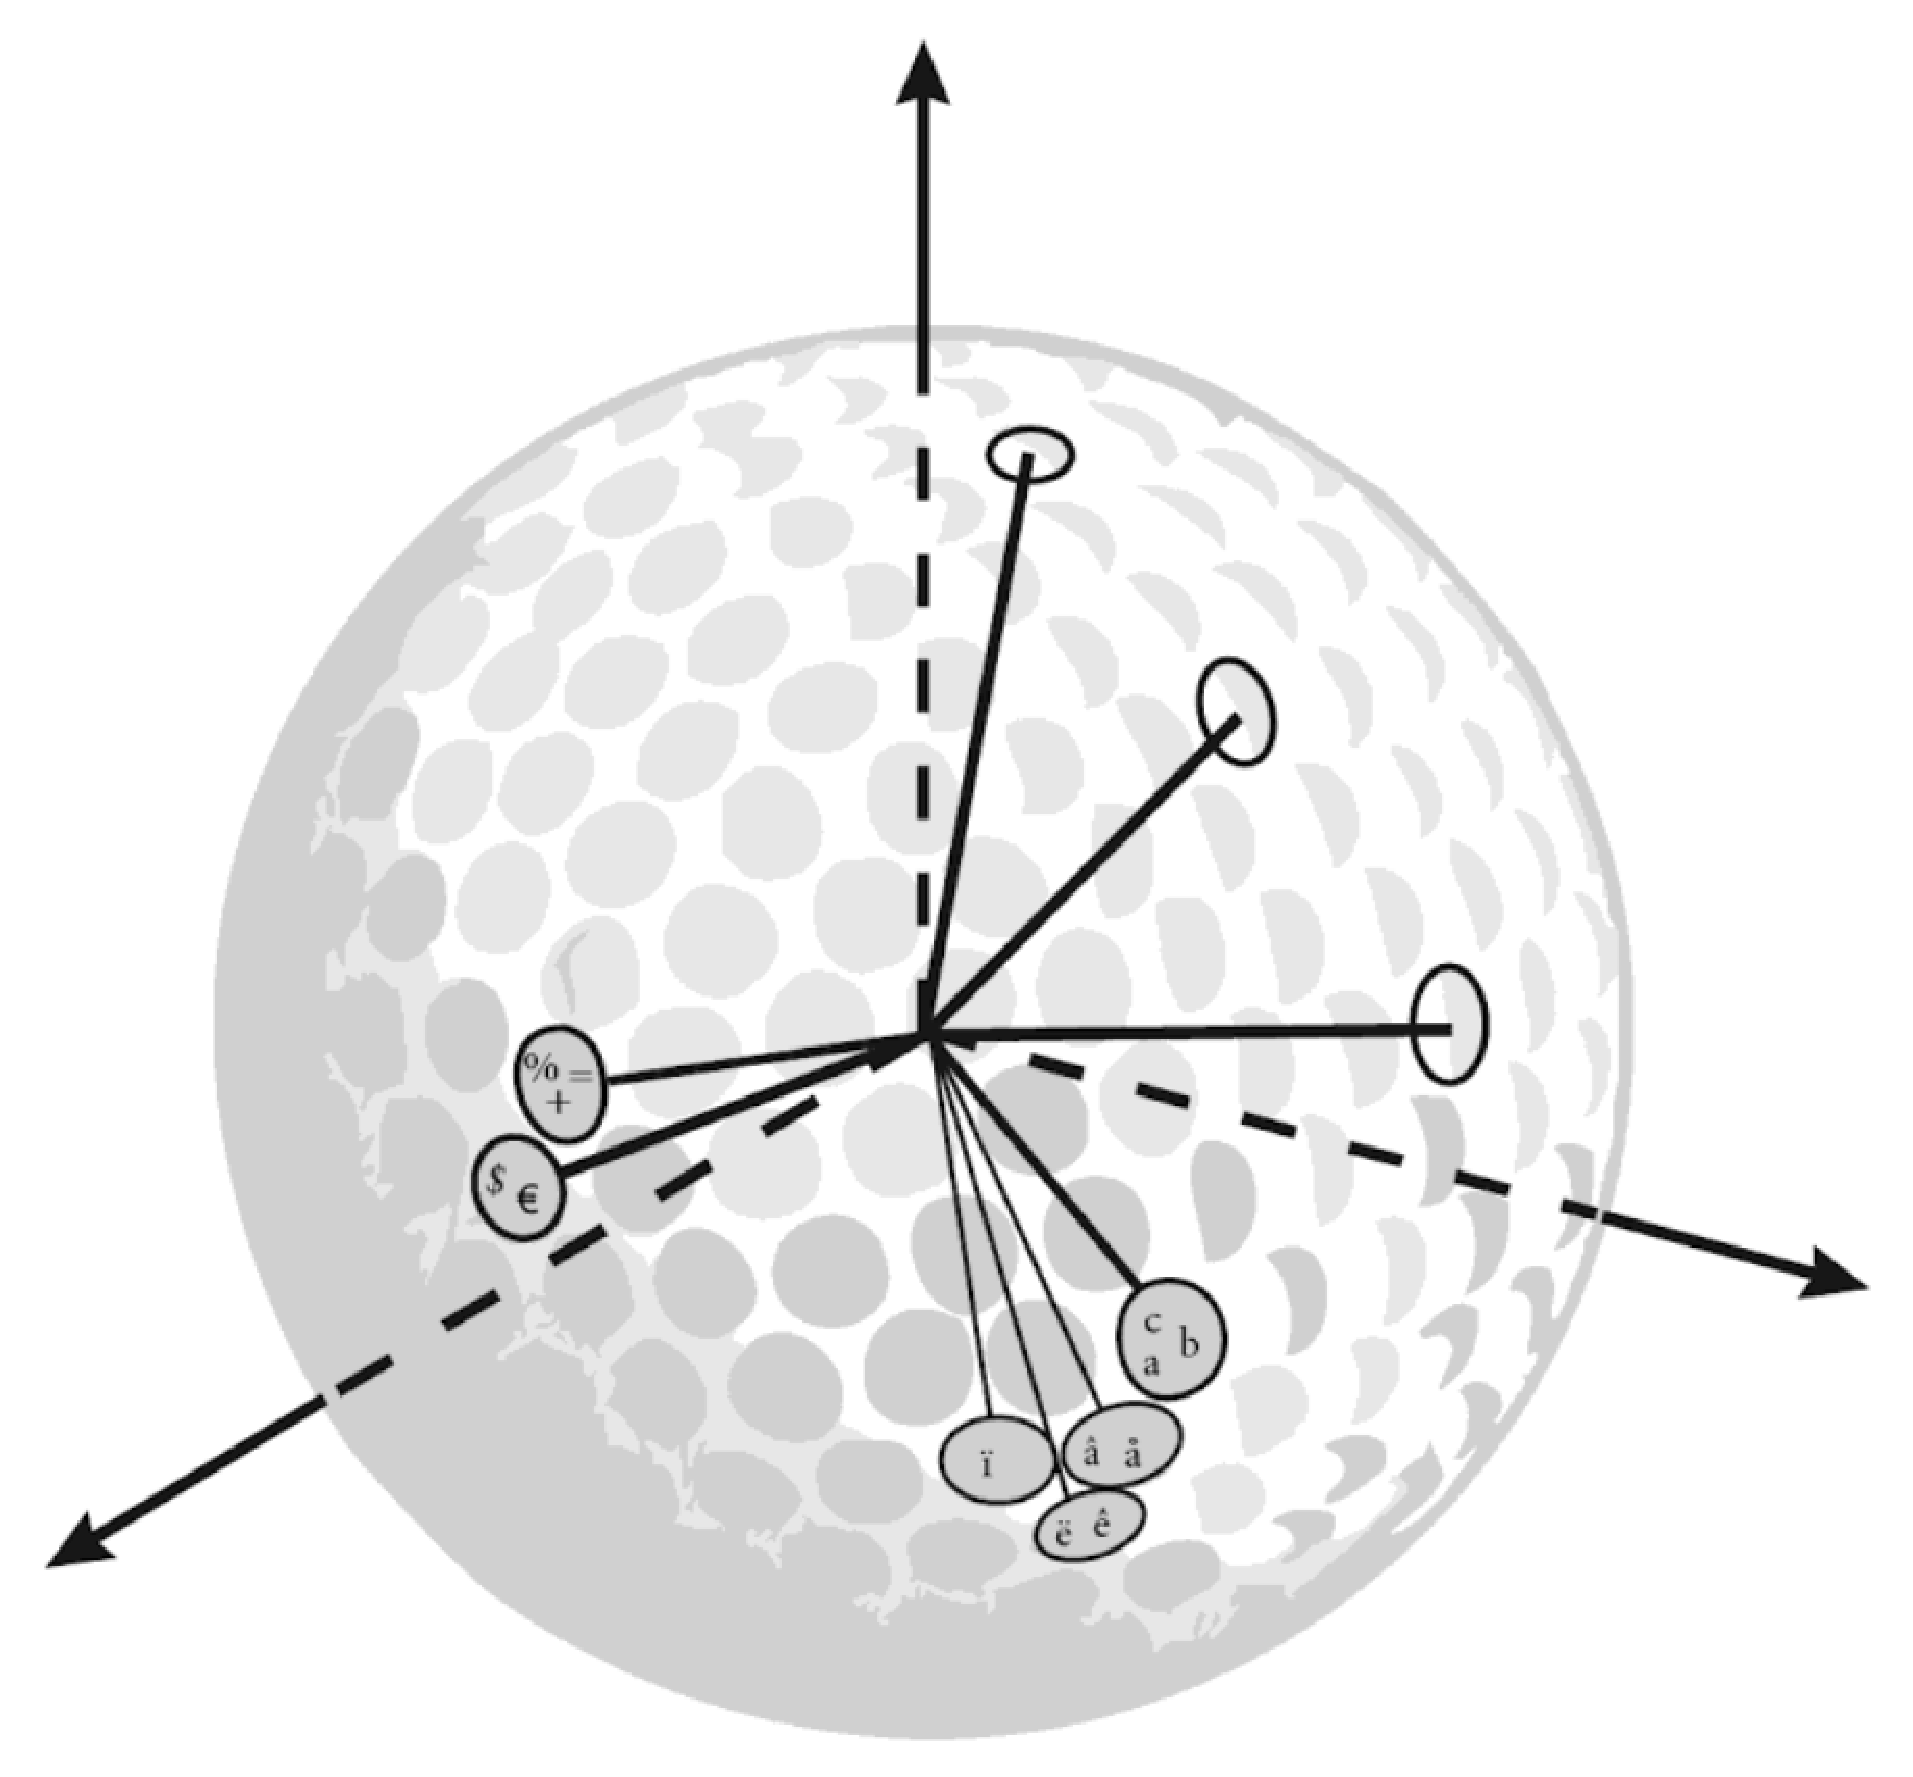
\includegraphics[width=0.45\textwidth]{imgs/conceptual_golfball.eps}
	}
	\subfloat[\label{subfig:constructed_vocab_sims}]{%
		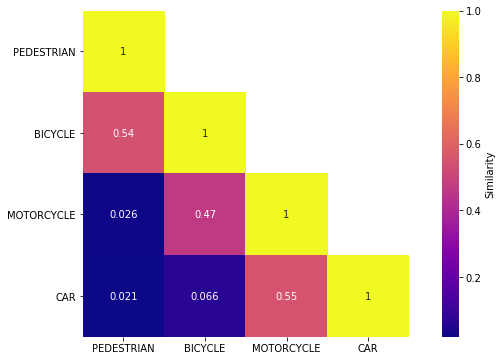
\includegraphics[width=0.45\textwidth]{imgs/SPA_constructed_vocab_sim.eps}
	}
	\caption{Aspects of vector vocabularies:~\protect\subref{subfig:conceptual_golfball} \enquote{Conceptual golf ball} depicting the idea of semantic vectors. Image source: \textcite{Eliasmith2013}.~\protect\subref{subfig:constructed_vocab_sims} Cosine similarities in a small, manually engineered vector vocabulary of dimension $256$.}
    \label{fig:vector vocabs}
\end{figure}

Let $\vartheta \subset \mathcal{S}(D)$ be a vocabulary in the $D$-dimensional \ac{SPA}, where each vector $v \in \vartheta$ represents one item, i.e., a symbol, word or concept, in the representational space.
The content and size, i.e., the items of interest to be represented in such a vocabulary and their number as well as the way the representing vectors are established is highly task-dependent.
In its simplest form, all vectors in the vocabulary are chosen at random.
This approach is feasible due to the properties of high-dimensional vector spaces (cf. Theorem~\ref{theorem:VSA_cossim_distribution} in section~\ref{sec:math_prop_vsas}) that the probability of randomly chosen vectors being dissimilar grows with vector dimension.
Therefore,  we have low probability of unintentionally confusing two different concept vectors.
However, this approach does not capture any similarities between items being represented.
Ideally, the goal is that the similarity between vectors in the vocabulary $\vartheta$ somewhat reflects the similarity between represented items.
Figure~\ref{subfig:conceptual_golfball} depicts this idea: one subset of the space is assigned to vectors representing letters whereas another subset contains vectors representing special characters.
For a small number of items, the simplest way to create a vocabulary respecting some kind of similarity is to manually engineer the desired properties from randomly chosen vectors.
Let us assume we want to derive representative vectors for four different classes of traffic participants, namely \emph{pedestrian}, \emph{bicycle}, \emph{motorcycle},  and \emph{car}.
A simple structured vocabulary could be constructed in the following way

\begin{align*}
\mathbf{PEDESTRIAN} &:= \mathbf{DRIVE} \varoast \mathbf{MUSCLE} + \mathbf{ACTUATOR} \varoast \mathbf{LEG} \varoast \mathbf{TWO} \\
\mathbf{BICYCLE} &:= \mathbf{DRIVE} \varoast \mathbf{MUSCLE} + \mathbf{ACTUATOR} \varoast \mathbf{WHEEL} \varoast \mathbf{TWO}\\
\mathbf{MOTORCYCLE} &:= \mathbf{DRIVE} \varoast \mathbf{MOTOR} + \mathbf{ACTUATOR} \varoast \mathbf{WHEEL} \varoast \mathbf{TWO}\\
\mathbf{CAR} &:= \mathbf{DRIVE} \varoast \mathbf{MOTOR} + \mathbf{ACTUATOR} \varoast \mathbf{WHEEL} \varoast \mathbf{FOUR},
\end{align*}
with $\mathbf{DRIVE}$, $\mathbf{MUSCLE}$, $\mathbf{MOTOR}$, $\mathbf{ACTUATOR}$, $\mathbf{LEG}$, $\mathbf{WHEEL}$, $\mathbf{TWO}$ and $\mathbf{FOUR} \in \mathcal{S}(D)$ all being atomic vectors chosen at random.
Figure~\ref{subfig:constructed_vocab_sims} shows the similarities in an example vocabulary in $\mathcal{S}(256)$ constructed in the aforementioned way.
This vocabulary is designed to map simple motion properties into a vector representation.
Thus, this manually engineered vocabulary yields the desired property that vulnerable road users (in this case pedestrians and bicyclists) are more similar to each other than motor vehicles, whereas there is also similarity between different types of cyclists.
This approach allows the engineer to encapsulate almost any desired kind of similarity without losing transparency during the encoding process, meaning that the reason for certain similarity artifacts is traceable.
However, not only does this approach become impracticable with increasing number of items in the vocabulary, it is also prone to biases imposed by the preferences of the human engineer.

A more sophisticated way to create a vector vocabulary is to learn it automatically from data.
In contrast to purely random vocabularies, the idea here is that the learning system is able to capture the intrinsic similarity between objects in the vector representation.
Again, the choice of learning paradigm (supervised vs.\ unsupervised) and architecture, e.g., \acp{CNN} or \acp{SOM}, depends not only on the given task, but also on the kind of similarity the vectors should encapsulate.
This can be visual similarity (e.g., items or objects that \enquote{look} similar), auditory similarity (e.g., objects producing similar sound), semantic similarity (e.g., words with similar meaning) or similarity in characteristics (e.g., similar motion characteristics).

\begin{figure}[t]
	\centering
	\resizebox{.9\textwidth}{!}{%
	\begin{tikzpicture}[%
	auto,
	multilayer,
	]
	% \Plane[x=0, y=0, width=5, height=2, opacity=1, style={dashed, color=red}, NoFill]
	\node[line width=1mm] (input) at (0,-6)
	{
\includegraphics[width=.15\textwidth]{imgs/mnist.png}};
	\draw[thick] (0,-5) -- (0.75, -3);
	\draw[thick] (0,-5) -- (0.25, -2.8);
	\draw[thick] (0,-5) -- (-0.25, -2.6);
	\draw[thick] (0,-5) -- (-0.75, -2.4);
	% \begin{Layer}[layer=1]
	% 	\draw[very thick] (0,0) rectangle (5,2);
	% 	\node at (-.5,-.5)[below right]{Layer 1};
	% \end{Layer}
	\Vertices{data/cnn_vertices.csv};
	\Vertices[Pseudo]{data/last_cnn_vertices.csv};
	\Edges{data/cnn_edges.csv}
	\Edge[Direct](41)(45)
	\Edge[Direct](42)(46)
	\Edge[Direct](43)(47)
    \Edge[Direct](44)(48)
    \path (36.north) -- (37.south) 
      node[midway, sloped, draw=red, 
           ellipse, 
           rotate=60,
           fit=(35)(38), 
           inner sep=2pt,
           xslant=-0.5,
           yslant=-0.5,
           ]{};
	\end{tikzpicture}
	}
	\caption{A schematic visualization of a \ac{CNN} network architecture with the second to last layer, whose activity can be considered a compressed, lower-dimensional representation of the high-dimensional visual input, highlighted by a red ellipsis.}
	\label{fig:cnn_arch}
\end{figure}

A similar approach to derive vectors representing digits from $0$ to $9$ was used in \textcite{Eliasmith2012} for the network performing the visual digit recognition task as part of the larger \ac{Spaun} model, which was derived by training a \ac{DBN} consisting of four \acl{RBM} layers.
This approach of using the activity of the second to last layer to generate atomic representational vectors can be generalized to any neural network for classification with dense layers at the end.
A typical way of learning a vocabulary whose vectors conserve visual similarity in supervised fashion are \acp{CNN}.
These network architectures are inspired by the human visual cortex and compress high-dimensional visual input to lower dimensional representations.
They usually consist of a series of convolutional and pooling layers followed by one or more fully connected layers, where the last layer provides the classification result (cf.\ Fig.~\ref{fig:cnn_arch}).
The activity of the second to last layer (the last fully-connected one before the actual classification) for each known class in the data set can be considered a representational vector for the current visual input.
A simple way of getting a representative vector for each class is simply calculating the element-wise, normalized mean over all examples in the test set.
We employ this approach in section~\ref{subsec:visual_vocabularies} to generate vocabularies encapsulating the visual similarity of traffic signs and traffic participants.

The aforementioned approach to create vector vocabularies encapsulating similarity by using neural networks, which are trained in supervised fashion, is suitable for capturing visual or auditory similarity structure in a vectors.
The generation of representational vectors for related or similar words or, more generally, semantic similarity in language is a problem often referred to as word embedding, which is a research question related to computational \acf{NLP}.
The most successful approaches such as \textit{word2vec} \parencite{Mikolov2013a, Mikolov2013} or \textit{\ac{GloVe}} \parencite{Pennington2014} typically use large corpora of text as input data and are trained in unsupervised fashion based on co-occurrence statistics of words.
The objective of those procedures aims at maximizing the dot product of word vectors that appear often in similar contexts while minimizing it for negative samples, which do not occur in the training data and thus are sampled at random.
For a given sentence $S=\left\{w_1, \ldots, w_n\right\}$, a context $C(w)$ of a word $w=w_i$ of size $k$ is a dynamic window of the form $C(w) = \left\{ w_{i-k}, \ldots, w_{i-1}, w_{i+1}, \ldots, w_{i+k}\right\}$.
The underlying assumption is that words sharing many contexts are similar to each other such that automated training with the aforementioned objective will produce a good word embedding.
Surprisingly, these learning procedures lead to linguistic regularities and algebraic relations between word vectors \parencite{Mikolov2013b}.
A common example is visualized in Fig.~\ref{fig:word2vec}: subtracting the vector representing $\mathbf{MAN}$ from the one representing $\mathbf{KING}$ and adding the vector representing $\mathbf{WOMAN}$ results in a vector most similar to the one representing $\mathbf{QUEEN}$, i.e., $\mathbf{KING} - \mathbf{MAN} + \mathbf{WOMAN} \approx \mathbf{QUEEN}$.
\begin{figure}[t]
	\centering
	\begin{tikzpicture}[%
	auto,
	scale=5,
	axis/.style={very thick, ->, >=stealth'},
	red line/.style={thick, ->, >=stealth', color=red},
	green line/.style={thick, ->, >=stealth', color=green},
	blue line/.style={thick, ->, >=stealth', color=blue},
	dashed blue line/.style={dashed, thick, color=blue},
	important line/.style={thick},
	dashed line/.style={dashed, thin},
	pile/.style={thick, ->, >=stealth', shorten <=2pt, shorten>=2pt},
	every node/.style={color=black}
	]
	% Draw axes
	% axis
	\draw[axis] (-0.5,0)  -- (1.2,0) node(xline){};
	\draw[axis] (0,-0.1) -- (0,1.1) node(yline){};
	\draw[red line] (0,0) -- (0.3, 0.8) node(King) [above right] {$\mathbf{KING}$};
	\draw[red line] (0,0) -- (0.7, 0.4) node(Man) [above right] {$\mathbf{MAN}$};
	\draw[green line] (0,0) -- (0.7, 0.9) node(Queen) [above right] {$\mathbf{QUEEN}$};
	\draw[green line] (0,0) -- (1.1, 0.5) node(Woman) [above right] {$\mathbf{WOMAN}$};
	\draw[blue line] (0,0) -- (-0.4, 0.4) node(KingMinusMan) [above] {$\mathbf{KING} - \mathbf{MAN}$};
	\draw[dashed blue line] (0.7,0.4) -- (0.3, 0.8);
	\draw[dashed blue line] (0.7,0.9) -- (1.1, 0.5);

	\end{tikzpicture}
	\caption{A typical example illustrating the semantic similarity structure between vectors representing the words \emph{king}, \emph{queen}, \emph{man} and \emph{woman} learned by Word2Vec allowing algebraic manipulation of the encoded entities. 
    Image inspired from \textcite{Mikolov2013b}.}
	\label{fig:word2vec}
\end{figure}
However, \textcite{Goldberg2014, Levy2015} point out that the formal reasons for successful learning of word embeddings of those approaches are not well understood.

\subsection{Encoding structure}
\label{subsec:encoding_struct}

In section~\ref{subsec:vocabs}, we have already seen that there are many ways to create vector vocabularies, that encode different types of similarity.
However, the strength of \acp{VSA} lies in the possibility to build structured representations from atomic vectors.
Unordered sets can be represented by simply adding up atomic vectors.
Through the properties of the similarity measure, the sum is similar to each vector contained in the sum.
The most common approach to incorporate structure is to use so-called role-filler pairs \parencite{Gayler2003}.
Such a pair is combined via the \ac{VSA}'s binding operation, where one vector of the pair takes the role of a variable while the other one can be considered the value of the variable.
We have already seen a simple example of this approach in section~\ref{subsec:vocabs}, where a small vocabulary representing four different classes of traffic participants was manually created.
In \ac{NLP} applications, this approach is useful when building up vectors representing phrases from a word vector vocabulary.
The phrase \textit{The dog chases the boy} could be encoded in a vector as
\begin{equation*}
	\mathbf{agent} \varoast \mathbf{dog} + \mathbf{verb} \varoast \mathbf{chase} + \mathbf{theme} \varoast \mathbf{boy},
\end{equation*}
assuming we already have a vocabulary containing atomic vectors representing those items.
Another typical example of this approach is the encoding of relations between items, such as \enquote{$\mathbf{A}$ is the mother of $\mathbf{B}$}.
This relation could be represented in vectors through
\begin{equation*}
	m \left(\mathbf{A}, \mathbf{B} \right) = \mathbf{motherof} + \mathbf{mother} \varoast \mathbf{A} + \mathbf{child} \varoast \mathbf{B}.
\end{equation*}
The strength of \acp{VSA} is that the vectors representing such relations can subsequently be manipulated and combined using the \ac{VSA}'s algebraic operations.
\textcite{Kanerva2000} shows that this approach can be used to create a system, that is able to infer one relation, which is induced by another relation, through learning from example.
Their example features the aforementioned \textit{mother of} relation, which induces the \textit{parent of} relation
\begin{equation*}
	p \left(\mathbf{A}, \mathbf{B} \right) = \mathbf{parentof} + \mathbf{parent} \varoast \mathbf{A} + \mathbf{offspring} \varoast \mathbf{B},
\end{equation*}
i.e., we have $m\left(\mathbf{A}, \mathbf{B}\right) \Longrightarrow p\left(\mathbf{A}, \mathbf{B}\right)$.
Combining several examples
\begin{equation*}
	M = \sum_{i=0}^{n} m\left(\mathbf{A}_i, \mathbf{B}_i \right) \varoast p\left(\mathbf{A}_i, \mathbf{B}_i \right)
\end{equation*}
yields a transition vector, which gives $ M \varoast m \left(\mathbf{X}, \mathbf{Y} \right) \approx p \left(\mathbf{X}, \mathbf{Y} \right)$ for unseen examples $\mathbf{X}$ and $\mathbf{Y}$.
However, this approach is based on the self-cancellation property (i.e., $\mathbf{X} \varoast \mathbf{X} = \pmb{1}$) in certain \acp{VSA} (in particular  \acp{BSC}), as it leads to $M$ containing the vector $\mathbf{motherof} \varoast \mathbf{parentof} + \mathbf{mother} \varoast \mathbf{parent} + \mathbf{child} \varoast \mathbf{offspring}$ \parencite[see][for details]{Kanerva2000}.
A similar approach was used in \textcite{Kleyko2015a} for a prototype of concept learning.
\textcite{Rasmussen2011} employ a similar approach to encode a rule for inductive learning in a transition vector using the \ac{VSA}'s algebraic operations to solve \acp{CogRPM}.
The authors represent consecutive cells in an \ac{CogRPM} and encode the transition from one cell to another in a particular transition vector and, from a sequence of those, iteratively create a general transition vector encapsulating the general rule for going to the next cell in the matrix.
They implement these vectors as well as their inductive learning system in a \ac{SNN} model, a process we will also briefly discuss in the next section,

\subsection{Implementation in \aclp{SNN}}%
\label{subsec:implementation_in_snns}

In this section, we show how \acp{VSA} and in particular the \ac{SPA} can be implemented in \acp{SNN}.
In section~\ref{subsec:nef_representation}, we have already discussed the representation principle of the \ac{NEF}, that allows to encode time-varying vectors in the activity of populations of spiking neurons using Equation~\eqref{eq:nef_encoding}.
Given that all representations of entities in the \ac{SPA} are vectors, we can directly apply Equation~\eqref{eq:nef_encoding} to encode any vector representation generated using the principles and algebraic operations of the \ac{SPA}.
Similarly, we can employ Equation~\eqref{eq:nef_decoding} to decode back out the original vector from the neurons' activities.
However, to manipulate the encoded vectors into structured representations using the \ac{SPA}'s algebraic operations, we also need to be able to implement these operations in networks of spiking neurons.
Again, the tools of the \ac{NEF} allow this implementation.
The implementation of element-wise addition of vectors is straightforward: assuming we have created populations $A$ and $B$ encoding the vectors $ \mathbf{v}$ and $ \mathbf{w}$ respectively using Equation~\eqref{eq:nef_encoding}, we can now use the transformation principle and Equation~\eqref{eq:nef_transformation} to connect \emph{both} populations $A$ and $B$ to a third population $C$ with both connections approximating the identity function.
The population $C$ receiving input from both populations $A$ and $B$ will end up representing an approximation of the sum $ \mathbf{v}+ \mathbf{w}$.

Similarly, we can use the \ac{NEF}'s principles to implement the \ac{SPA}'s binding operation, circular convolution, in a network of spiking neurons.
Revisiting Equation~\eqref{eq:conv_with_dft}, we can write the circular convolution $ \mathbf{z} = \mathbf{v} \varoast \mathbf{w}$ of two vectors $\mathbf{v},\mathbf{w}$ as

\begin{equation}
    \mathbf{z} = \mathbf{v} \varoast \mathbf{w} = \ac{IDFT}\left(\ac{DFT}( \mathbf{v}) \odot \ac{DFT}( \mathbf{w}) \right). \tag{\ref{eq:conv_with_dft} revisited}
\end{equation}

We can consider the \ac{DFT} and \ac{IDFT} as linear functions given by the matrices

\begin{equation}
\label{eq:dft_mat}
W = \frac{1}{ \sqrt{D-1}} \left(\zeta_{D} ^{i\cdot j}\right)_{i,j=0}^{D-1}, \qquad
W^{-1} = \frac{1}{ \sqrt{D-1}} \left(\zeta_{D} ^{-i\cdot j}\right)_{i,j=0}^{D-1}
\end{equation}
and thus write circular convolution as matrix multiplication

\begin{equation}
\label{eq:circ_conv_mat}
\mathbf{z} = \mathbf{v} \varoast \mathbf{w} = W^{-1} \left( \left(W \mathbf{v}\right) \cdot \left(W \mathbf{w}\right)\right).
\end{equation}
Applying the \ac{NEF}'s transformation principle, we can implement circular convolution in a spiking neuron substrate.
To finally be able to unbind vectors, i.e., calculate $ \mathbf{v} = \mathbf{z} \varoast \bar{\mathbf{w}}$ using the pseudo-inverse element $ \bar{ \mathbf{w}} = \left(w_0, w_{D-1}, w_{D-2}, \ldots, w_{1}\right)$ (cf.\ Lemma~\ref{lemma:spa_pseudo_inv}), we can adapt Equation~\eqref{eq:circ_conv_mat}.
The function transforming a vector into its pseudo-inverse element is a simple permutation of elements given by the matrix 
\begin{equation}
\label{eq:mat}
C_{pinv} = \left(
    \begin{matrix}
        1 & 0 &  \cdots & 0  & 0 \\
        0 & 0 &  \cdots & 0  & 1 \\
        0 & 0 &  \cdots & 1  & 0 \\
        \vdots & \vdots  & \iddots & \vdots  & \vdots \\
        0 & 1 &  0 & \cdots  & 0 
    \end{matrix}
\right),
\end{equation}
which allows us to transform Equation~\eqref{eq:circ_conv_mat} into
\begin{equation}
\label{eq:unbind_mat}
\mathbf{v} \approx \mathbf{z} \varoast \bar{ \mathbf{w}} = W^{-1} \left( \left(W \mathbf{z}\right) \cdot \left(W \cdot C_{pinv} \mathbf{w}\right)\right).
\end{equation}
The implementation of a \ac{SNN} performing a biologically plausible version of a cleanup memory employing the \ac{NEF} is shown in \textcite{Stewart2011}.
Thus, applying the principles of the \ac{NEF}, we can represent the representational vectors of the \ac{SPA} in the activity of populations of spiking neurons and implement its algebraic operations in networks of spiking neuron populations.
A subtle detail worth noting with regard to implementing \acp{VSA} in \acp{SNN} is that the vectors used for representing concepts or entities of interest are \emph{not} vectors of neural activity.
That is, there are two distinct representational vector spaces: the space of neural activities (i.e., measurable properties like spike patterns) and the vector space used to generate the vocabulary and structured representations vectors, which in turn are represented by the activities of populations in the neural space \parencite[see][for further details]{Eliasmith2013}.

There are several reasons for implementing cognitive architectures like the \ac{SPA} in a spiking neuron substrate.
Regarding the application of vector-based representations in cognitive modeling, it makes sense to consider an implementation in neural activity, since the biological systems able to perform cognitive tasks are also systems of neural networks.
Hence, when generating models of some cognitive function or behavior such as the model for inductive rule generation applied to \acp{CogRPM} in \textcite{Rasmussen2011}, implementation in a spiking neuron substrate allows to compare the model's neural activity with neural activity measured in the brain of human subjects performing a similar task.
Such a comparison enables more detailed model analysis and improvements by allowing researchers to draw inspirations from actual biological systems.
Considering applications of the \ac{SPA} in domains such as automated driving as proposed in later chapters~\ref{chap:driving_context_classification},~\ref{chap:behav_pred} and~\ref{chap:mix_online_learning}, the possibility of implementation in a spiking neuron substrate is particularly interesting in terms of energy-efficiency.
As discussed in section~\ref{sec:neuromorphic_HW}, there exists a growing number of neuromorphic hardware devices dedicated to efficiently processing networks of spiking neurons.
Such dedicated computing hardware allows to run \acp{SNN} more efficiently than traditional computing hardware, which often requires several orders of magnitude less energy \parencite{Hunsberger2016}.
This is particularly interesting in mobile applications such as robotic systems or, more particularly, automated driving, which poses increasingly strong restrictions on the energy-budget of individual components due to growing setups of both, on-board sensors and computing hardware.
Since these novel computing devices are not yet available as commercial products but rather prototypes developed in academic research, the deployment of the models developed in this thesis on neuromorphic computing hardware integrated into a vehicle's architecture is unfortunately out of scope of this thesis. 

\section{Summary}
In this chapter, we have introduced the theoretical background and mathematical properties of \aclp{VSA}, which is the basis for subsequent chapters.
Furthermore, we established a formal, mathematical notion for \acp{VSA} in general (section~\ref{sec:math_prop_vsas}), which, to the best or our knowledge, is not available in the literature except for treatments of particular instantiations of \acp{VSA} such as in \textcites{Plate1994}{Gayler1998}{Kanerva2009}.
Then, we shifted our focus to one particular \ac{VSA}, the \ac{SPA}, presenting its most important aspects and properties with respect to subsequent chapters of this thesis.
Furthermore, we gave a brief description of the \acl{NEF}, which is typically used to implement large-scale neural models of spiking neurons such as the one presented in \textcite{Eliasmith2012}.
Finally, we have introduced the basic principles of cognitive modeling using \acp{VSA} in general and the \ac{SPA} in particular.
We showed several general approaches to generate vocabularies of atomic vectors, which form the basis of more complex structured representations, which are built from the vocabulary using the \ac{VSA}'s algebraic operations.
Finally, we connected the mathematical description and theory of both, the \acp{VSA} and the \ac{NEF} by depicting how the \ac{NEF} can be used to implement the \ac{SPA} in a spiking neuron substrate, which offers interesting possibilities regarding energy-efficiency in mobile applications such as automated driving.
We will use the theory and findings shown here in subsequent chapters to derive vector-based representations of automotive data measured and collected in actual driving situations to tackle tasks like classifying the current driving context or prediction the future development of the scene based on past observations.

\chapter{Distributed representations of automotive scenes}%
\label{chap:a_cognitive_approach_to_represent_automotive_scenes}

In chapter~\ref{chap:research_context} and especially in section~\ref{subsec:knowledge_representation}, we have seen that, already today, there is a plethora of \acfp{ADAS} in intelligent vehicles. 
In future vehicles, the number of modules tackling different sub-tasks necessary to enable (semi-) autonomous driving and to interact with humans inside and outside the car will increase even more.
Given the complexity of the physical world and the recent success of \acp{DNN} in diverse applications, a substantial amount of such modules could be data-driven with increasingly large neural networks under the surface.
In a worst case scenario, each of these systems will encapsulate its own representation of knowledge about the data it processes in complete separation from other, potentially related, systems.
Typically, the representations used rely completely on numerical values and lack possibilities to be enriched or combined with symbol-like representations.
On the other hand, increasingly deep neural network architectures are not only hungry for data to generalize sufficiently beyond the examples they have been trained on, but also tend to require a substantial amount of computational resources.
Although this aspect is more severe for the training process, it becomes more important for mobile applications such as automated vehicles during the deployment phase.

In this thesis, we propose a novel representation for automotive scenes based on modern cognitive modeling techniques, namely the \ac{SPA}.
The \ac{SPA} is one particular example from a family of cognitive architectures commonly referred to as \acp{VSA} (see section~\ref{subsec:vector_based_approaches} and chapter~\ref{chap:introduction_to_vsas} for further details).
One of the key components of these cognitive architectures is to use high-dimensional vectors for representation.
This representational approach offers several desirable features.
High-dimensional vectors are one variant of distributed representations in the sense that information is captured over all dimensions of the vector instead of one single number.
This aspect makes distributed representations more robust to noise in the sense that a few noisy entries influence the overall information carried by the vector less compared to low-dimensional representations.
Furthermore, vector representations allow to encode both, symbol-like and numerical structures in a similar and unified way.
Additionally, the algebraic operations enable manipulation and combination of represented entities into structured representations.
One potential advantage of this approach is that the number of dimensions remains fixed independent of the number of entities combined through the architecture's algebraic operations.
Finally, vectors are a suitable representational substrate to be used in combination with neural networks.
On the one hand, vectors are a natural input to classic \acp{ANN}, but they also offer the possibility to be efficiently implemented in \acp{SNN} using the principles of the \ac{NEF} \parencite[see][but also section~\ref{subsec:implementation_in_snns}]{Eliasmith2013}.
Given a widespread implementation of the representations proposed here in combination with \acp{SNN} as algorithmic substrate within intelligent vehicles, the latter offers the potential to deploy such neural representations on dedicated neuromorphic hardware (cf.\ section~\ref{sec:neuromorphic_HW}).
Although neuromorphic computing hardware as well as the corresponding neural algorithms are mainly used in academic research and often lack the technical maturity required by industrial applications, they show promise to be an energy-efficient option for future automated vehicles once reaching the required level of maturity.

\begin{figure}[t]
    \centering
    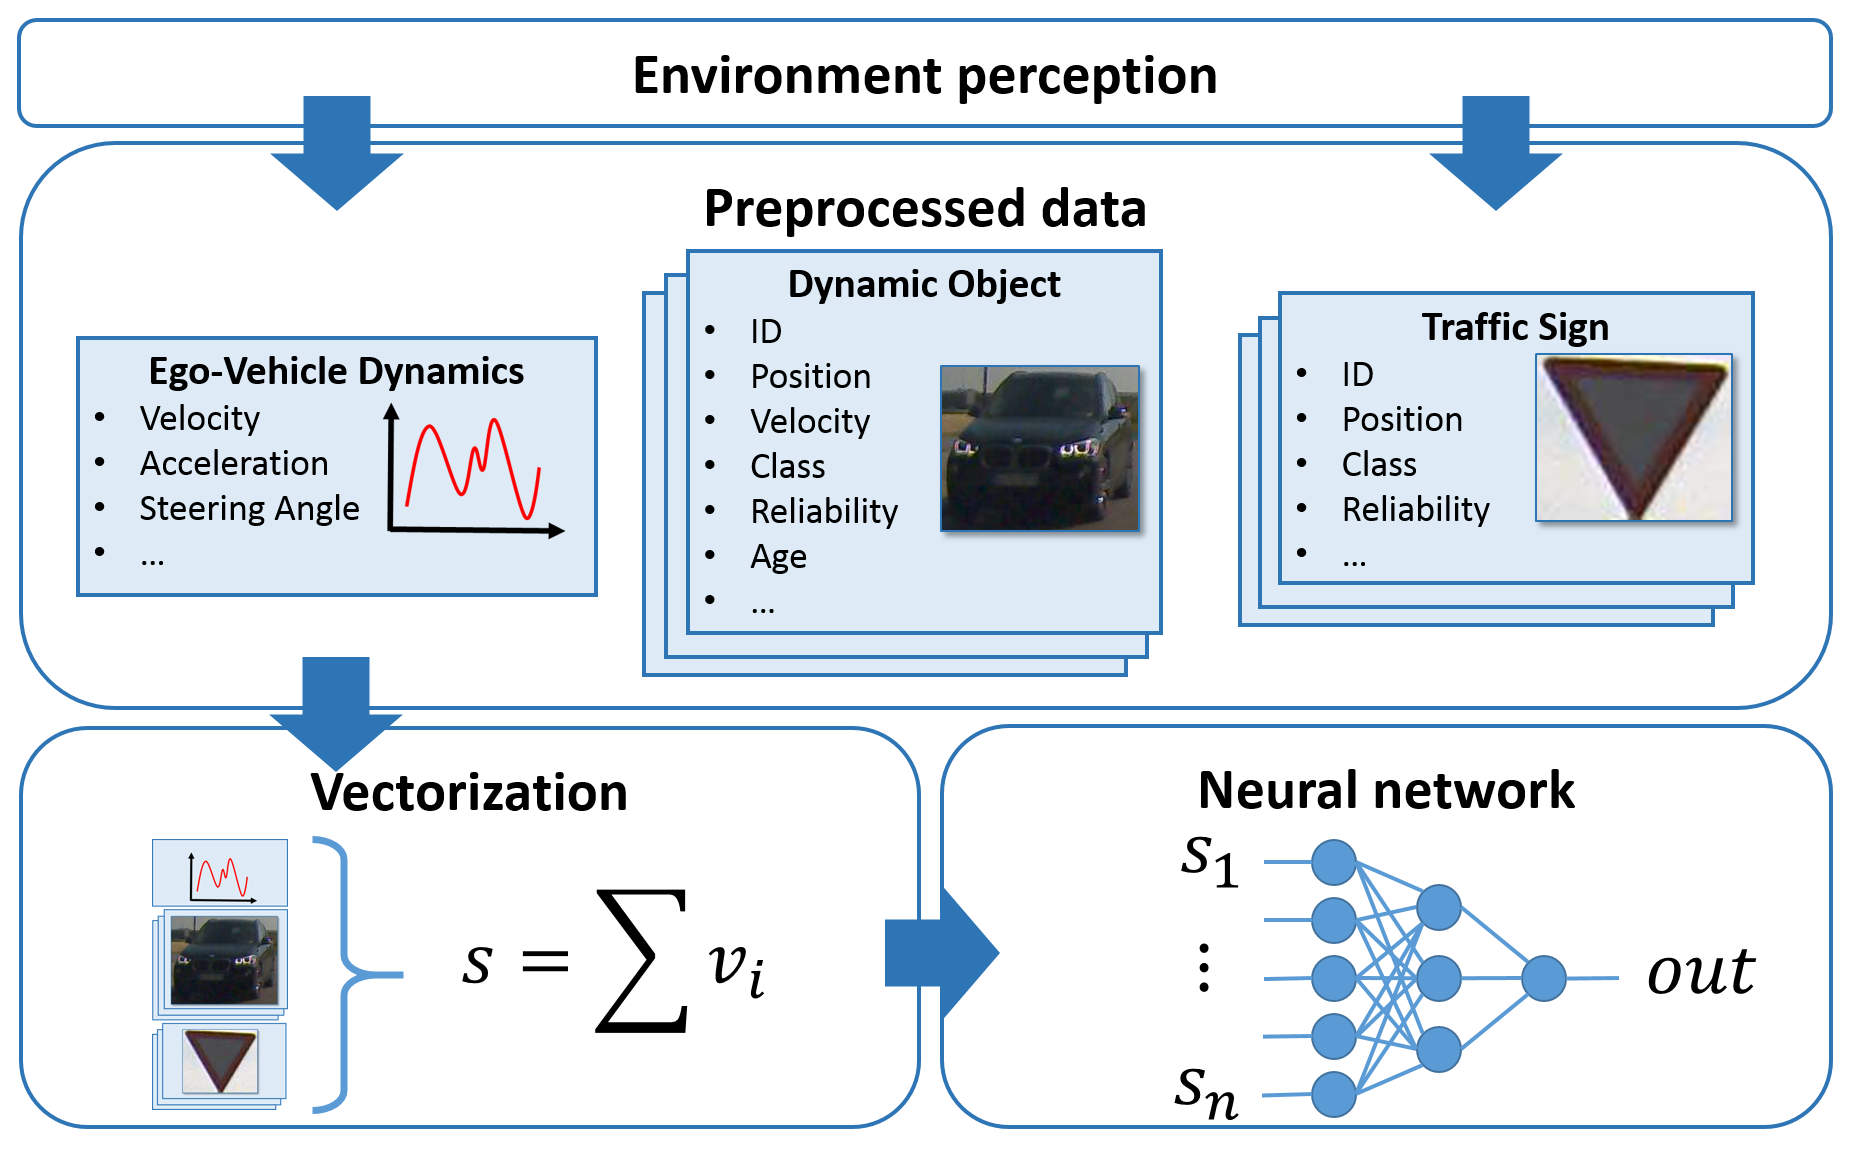
\includegraphics[width=0.8\linewidth]{imgs/system_overview_horizontal.eps}
    \caption{Visualization of the general flow of information of our proposed approach.}
    \label{fig:vectorization}
\end{figure}

In this chapter, we introduce our proposed approach to encapsulate high-level information about automotive scenes in high-dimensional, semantic vectors using the \ac{SPA} as representational substrate.
For this encoding phase, we follow the first two stages, namely \emph{preprocessing} and \emph{representation generation}, of the three-stages process established in \textcite{Gallant2013}.
The third and final stage, \emph{output computation}, will be the subject of subsequent chapters, where we investigate concrete applications and use cases.
The preprocessing stage is the step of creating a suitable vector vocabulary, whereas the representation generation stage is the process of building up structured representations from the atomic vectors within the vocabulary.
Furthermore, we analyze how different types of data could be encoded in such a representation, we show possible variations of how to encapsulate data in vectors and how they influence the final representation.
We also investigate potential limitations imposed by such representations to provide insights into how many concepts can be efficiently encoded in our representations without loss of information.  


\section{Preprocessing stage - generating a vocabulary}%
\label{sec:preprocessing_stage_generating_a_vocabulary}

Figure~\ref{fig:vectorization} visualizes the general flow of information of our proposed system.
To represent high-level information about a scene in an abstract vector representation, we work with already processed data, which comes either from individual sensors performing their own low-level processing, or from a higher-level, central module already fusing information from several sensors.
We simply refer to this step as \emph{environment perception} in Fig.~\ref{fig:vectorization}, whereas its output is referred to as \emph{preprocessed data}.
This data is typically available as lists of objects present in the current scene and is translated into a semantic vector representation by first assigning atomic vectors to entities of interest and then building up more complex, structured representations by using the \ac{SPA}'s algebraic operations.
In this section, we will investigate the first step of assigning atomic vectors to entities of interest, i.e., creating a suitable vector vocabulary.
We have already seen in section~\ref{subsec:vocabs} that such vocabularies can be created in several different ways, which we will here investigate with the specific focus of encoding automotive scenes.

\subsection{What types of data to encode?}%
\label{subsec:what_types_of_data_to_encode_}

The data to be encoded in a semantic vector substrate depends not only on the information available from the current sensor-setup, but also on the task at hand.
For instance, if we want to classify the current driving context (like in chapter~\ref{chap:driving_context_classification}), the relevant information might be different to the task of predicting a vehicle's trajectory (like in chapter~\ref{chap:behav_pred}).
Here, we give an overview of what information in general is available in an intelligent vehicle and how to encode it in a semantic vector substrate.
We distinguish between symbol-like information such as the type of a dynamic object or numerical information such as the current acceleration of the ego-vehicle.
In this section, we focus mainly on the symbol-like information, which is suitable to be represented using a single atomic vector or an algebraic combination of several atomic vectors.
In section~\ref{subsec:different_vector_representations_for_numerical_values}, we will focus on numerical information and different options of encoding them in vectors.
Here, we will closely follow the structure of section~\ref{sec:cognitive_modelling_with_vsa} and present different possibilities to generate a vocabulary of atomic vectors to built structured representations upon.

If the vectors in the vocabulary are not chosen at random, the general goal when creating the vocabulary is to generate atomic vectors that carry inherent structure or meaning.
This meaning is typically reflected by similar concepts being mapped to similar vectors.
However, there are several possible notions of similarity that can be encoded in the vocabulary, which we will specify in this section.

\subsubsection{Visual similarity}%
\label{ssubsec:visual_similarity}

A first simple and comprehensible notion of similarity is visual similarity between two entities: \enquote{do they look similar}. 
Encoding this notion in vectors, we would expect the vector representations to encapsulate this type of similarity within the relation between the vectors, meaning that vectors representing visually similar entities will have large cosine similarity.
In conjunction with other information, this type of similarity could be useful to detect a wrong classification, in case it has high similarity to another one that makes more sense in the situation or context at hand.
An example would be the German traffic signs indicating a speed limit of \SI[per-mode=symbol]{30}{\kilo\meter\per\hour} and \SI[per-mode=symbol]{80}{\kilo\meter\per\hour}, which are both circular with a red frame and a similar looking black number on white background in the middle.
However, encountering a speed limit sign of \SI[per-mode=symbol]{30}{\kilo\meter\per\hour} in an urban situation is more plausible than a sign indicating a speed limit of \SI[per-mode=symbol]{80}{\kilo\meter\per\hour}.

\subsubsection{Similarity of motion}%
\label{ssubsec:similarity_of_motion}

Another notion of similarity, that is a candidate to be encoded in a vector vocabulary, is the similarity of motion properties.
For instance, bicycles and motorcycles have more similar motion properties (dynamics of vehicles with two wheels) than for example a pedestrian and a truck.
Apart from motion properties such as dynamics of the movement, the number of wheels or the mean expected velocity, the direction of movement of traffic participants can be also a notion of similarity to be encoded in the vocabulary.
For instance, traffic participants such as bicycles or cars moving towards us might be encoded more similarly to each other than to parked cars or those moving away.
Furthermore, some entities are more likely to change their motion or direction: while traffic lights frequently alternate and parked cars might start moving, trees, buildings and traffic signs are expected to remain static. 
The notion of similarity of motion can be useful in various ways.
In a first step, knowing the motion of other traffic participants could help in classifying the situation: on a multi-lane highway we would expect cars around us to move in the same direction, whereas in an urban driving situation, the motion of other traffic participants is more diverse. 
Additionally, this notion of similarity could potentially help in focusing the system's attention or, more precisely, use computing power more efficiently on entities that are more relevant to decision making.
For example, a change of the \enquote{motion status} (e.g., when a bus stops) might need particular attention.

\subsubsection{Semantic similarity}%
\label{ssubsec:semantic_similarity}

While visual similarity already captures a significant part of perceivable information about entities in automotive context, there is further information, that could be encoded in the vector vocabulary and that is different, or maybe even contrary to visual similarity. 
Considering automotive situations, we as humans do not only assess them based on visual appearance but also by incorporating underlying and, most likely, previously acquired knowledge about the objects in the scene.
This underlying information can be considered the semantic aspect.
Revisiting the aforementioned example, the speed limit sign for \SI[per-mode=symbol]{30}{\kilo\meter\per\hour} is \emph{visually} more similar to \SI[per-mode=symbol]{80}{\kilo\meter\per\hour} than to \SI[per-mode=symbol]{20}{\kilo\meter\per\hour}.
However, in the context (or semantics) of an automotive situation such as driving in an urban environment, speed limit signs for \num{20} and \SI[per-mode=symbol]{30}{\kilo\meter\per\hour} should be contextually or semantically more similar to each other than signs for \num{30} and \SI[per-mode=symbol]{80}{\kilo\meter\per\hour}, since they are more likely to appear in similar contexts and both describe the traffic rule restricting driving to slow velocities.

Semantic similarity is not quite as intuitive as visual similarity. 
In general, we want to encode objects and concepts sharing similarity in \emph{meaning} in vectors with a high cosine similarity.
However, it is not intuitively clear what similar meaning actually refers to and how to properly define semantic similarity in an automotive context.
In the field of generating word embeddings for natural language processing, the typical assumption is that words sharing similarity in meaning appear in close proximity with high probability within text corpora.
This assumption could be transferred to automotive context as well, for instance, thinking of traffic signs indicating speed limits appearing in similar contexts or driving situations.
For example, traffic signs indicating moderate speed limits are more likely to appear in urban driving situations compared to higher speed limit signs being less likely to appear in such a context.
However, on the one hand, it is not clear how to transfer this approach to other object classes such as traffic participants, whose appearance probability is less context dependent than for traffic signs. 
On the other hand, the process of automatically training a system to learn this form of embedding is not clear as it would probably demand for another learning model to extract contextual information from the rich features of driving contexts.
Therefore, we will now focus on the potential meaning of objects appearing in an automotive environment and how their semantic meaning could be embedded into a vector representation while leaving aside intangible concepts representing vehicle dynamics such as \emph{velocity} or \emph{acceleration}.

\paragraph{Traffic signs}%
\label{par:traffic_signs}

Any traffic sign carries an explicit meaning defined in traffic law and anyone with a driver's license should know its meaning and be able to immediately explain it.
The meaning of a traffic sign is an instruction for the driver's behavior to, for instance, not surpass a certain velocity or to give way to other traffic participants. 
There are sub-groups of signs with similar meanings such as signs indicating speed limits, prescribed direction or warnings for potentially dangerous road conditions or to pay increased attention.
Encoding the semantic structure of traffic signs in a vector vocabulary, we expect not only all traffic signs will be similar but also that all signs within a certain sub-group end up being more similar to one another compared to signs from other subgroups. 
For instance, signs indicating speed limits should be similar to one another, ideally with signs indicating lower velocities such as \SI[per-mode=symbol]{20}{\kilo\meter\per\hour} and \SI[per-mode=symbol]{30}{\kilo\meter\per\hour} should be more similar than \SI[per-mode=symbol]{30}{\kilo\meter\per\hour} and \SI[per-mode=symbol]{130}{\kilo\meter\per\hour}. 
Beside their explicit meaning, the number of traffic signs is finite and limited to a small number compared to the number of words in a typical human-level language vocabulary.
Therefore, it is possible to manually engineer their semantic similarity, which makes it easier to impose our human understanding onto the structure, although the resulting vocabulary will most likely differ from the structure an unsupervised learning model would pick up from the data. 

\paragraph{Traffic participants}%
\label{par:traffic_participants}

While the meaning of traffic signs is clear and explicit, it is far more difficult to derive a meaning of a traffic participant such as a car or a pedestrian or a measure of similarity between them.
It is unclear if a truck is semantically more similar to a motorcycle or to a car without considering any contextual information while ignoring similarity of motion properties, which have already been discussed in section~\ref{ssubsec:similarity_of_motion}.
However, if we do consider contextual information, we as humans decide intuitively if a truck and a motorcycle are more similar when compared to a pedestrian by, e.g., considering their velocity of motion or their vulnerability.
We also know from experience that the meaning of a car approaching from the right potentially means that it has the right of way when we encounter a situation at a crossroads without traffic signs indicating other right of way rules. 
Hence, the situational context has a significant impact on comprehending the \emph{meaning} of traffic participants, which in most cases directly results in appropriate driving actions to take such as decelerating or changing the lane.
However, such a situational understanding is impossible to derive without additional information such as position, velocity or direction of each traffic participant.
Consequently, it is impossible to encapsulate such semantic or contextual similarity in a vector vocabulary directly but rather encode another notion of similarity for atomic vectors of traffic participants and built situational similarity through structured representations using the \ac{VSA}'s algebraic operations.

\subsubsection{Summary on similarity}%
\label{ssubsec:summary_similarity}

All of the aforementioned notions cover a certain aspect of similarity.
Ideally, it is desirable for a vector vocabulary to encapsulate more than one notion of similarity comparable to a human understanding all these different aspects of similarity.
However, it is not clear if it is helpful or even possible, to encapsulate several notions of similarity into one coherent vector vocabulary or if it is more suitable to have separate vocabularies for each similarity of interest and combine them in structured representations using the \ac{VSA}'s algebraic operations as mentioned, e.g., in \textcite{Crawford2016}.
For the remainder of this section, we give an overview over different options of how to generate vector vocabularies encoding their own notion of similarity.

\subsection{Random and manually engineered vocabularies}%
\label{subsec:basic_random_vocabularies}

The simplest possible option to generate a vocabulary of atomic vectors is to sample them randomly, in case of continuous \acp{VSA} such as the \ac{SPA}, from the $D$-dimensional unit sphere \parencite{Voelker2017}.
Naturally, randomly chosen atomic vectors do not carry semantic meaning or any intended notion of similarity.
However, given a sufficiently large dimension $D$ of the chosen \ac{VSA} and its theoretical properties (see chapter~\ref{chap:introduction_to_vsas}), we can assume that randomly chosen vectors will be dissimilar enough to avoid accidentally mistaking them for one another.
Another advantage of this simple approach is that it is comparatively easy to create a vocabulary avoiding any complex learning system to embed the concepts of interest in semantic vectors.
On the other hand, if specific applications demand for the vectors to actually carry semantic information meaning that similar concepts need to be mapped to similar vectors for the application to succeed, this simple approach can be extended by manually engineering a vocabulary reflecting the desired similarity structure.
This is typically achieved by randomly choosing a set of auxiliary vectors and building atomic vectors with the desired similarity from them through the \ac{VSA}'s algebraic operations (cf.\ section~\ref{subsec:vocabs}).
However, this approach is only feasible and appropriate for rather small sized vocabularies since manually designing semantic vectors with certain similarity properties becomes intractable quickly with an increasing number of concepts to be embedded.
Furthermore, manually designing vocabularies involves design choices by human engineers, which is sensitive to potentially undesired biases in the similarity structure of the vectors.
For instance, the example vocabulary created in section~\ref{subsec:vocabs} solely focused on the motion characteristics and typical actuators of different traffic participants.
However as mentioned before, there are many other possible similarity structures such as visual (or auditory), motion or semantic similarity, to be considered when designing the vocabulary.

\subsection{Visual vocabularies}%
\label{subsec:visual_vocabularies}

The next step to generate vocabularies with an inherent similarity structure is to encapsulate visual similarity in a vector embedding.
Visual similarity is an intuitive concept and we can make an educated guess that this notion of similarity could be beneficial for several tasks when encoded directly in the vector vocabulary. 
However, it is preferable to automatically learn to embed visual similarity in vectors instead of manually engineering the similarity between entities as this approach does not scale well for an increasing number of items to be encoded.
One option for such an automated learning system to generate a structured vocabulary encoding visual similarity is to adapt a \acf{DNN} for image classification.
Such a neural network can be thought of as an efficient image compression machine.
While earlier and intermediate layers learn sensibility to visual features such as edges and shapes, the information in the image is compressed into a single dimension, namely the label, at the final classification layer.
Considering the special case of a \acf{CNN}, one option would be to simply use the output of one of the later fully-connected layers and regard it as a vector since we expect the vectors of visually similar images to be similar regarding their cosine similarity.
Here, we focus our efforts of generating a visual vector vocabulary on items of interest to automated driving, namely the aforementioned categories of traffic signs and traffic participants.

\subsubsection{Traffic signs}%
\label{ssubsec:traffic_signs}

\begin{figure}[t]
    \centering
    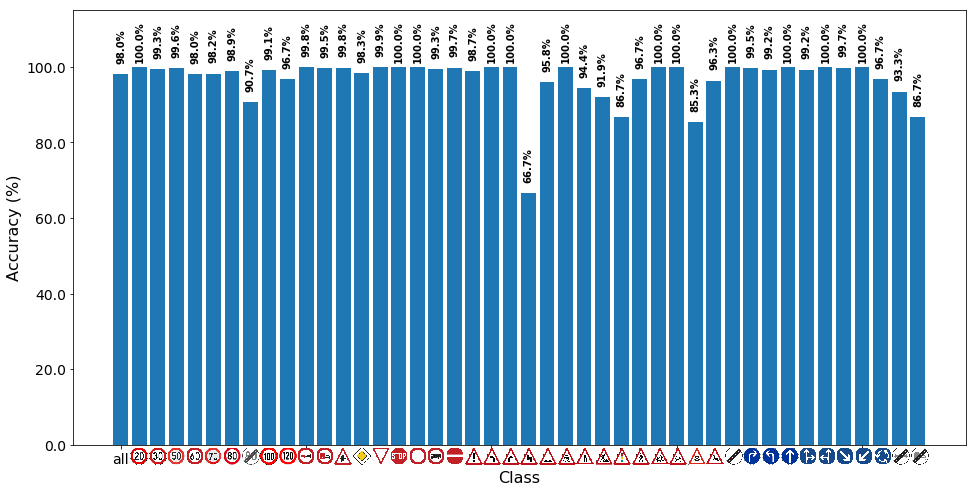
\includegraphics[width=1.\linewidth]{imgs/CNN_GTSRB_performance_plot.eps}
    \caption{Accuracy performance of the \ac{CNN} for traffic sign classification on the test part of the \ac{GTSRB} data set for all traffic signs (most left bar) and all individual traffic signs.}
    \label{fig:CNN_GTSRB_performance_plot}
\end{figure}

To achieve the task of encoding traffic signs encountered by an automated vehicle, we employ a variant of the state-of-the-art \ac{CNN} for traffic sign classification proposed by \textcite{Ciresan2012}.
We train a simplified version of this network on the \acf{GTSRB} \parencite{Stallkamp2012}, which is a data set including a total of \num{51840} images of \num{43} different classes of traffic signs.
Although the \ac{GTSRB} data set does not contain all possible traffic signs, it is a suitable and sufficiently large data set for our purposes of learning a visual vector vocabulary.
The original multi-column network proposed by \textcite{Ciresan2012} combines several variants of the same network architecture trained on the original input images as well as four different, high-contrast normalized versions of the input images by averaging the predictions of all individual networks.
For simplicity, we only use a single-column version of this network to generate a visual vector vocabulary. 
Figure~\ref{fig:CNN_GTSRB_performance_plot} shows the classification accuracy of our network on the test part of the \ac{GTSRB} data set for all traffic signs (most left bar) and all individual signs.
The network achieves competitive results with \SI{98}{\percent} classification accuracy on all traffic signs while detecting all but four traffic signs with accuracy values way above \SI{90}{\percent}, which is sufficient for our purposes.

\begin{figure}[t]
    \centering
    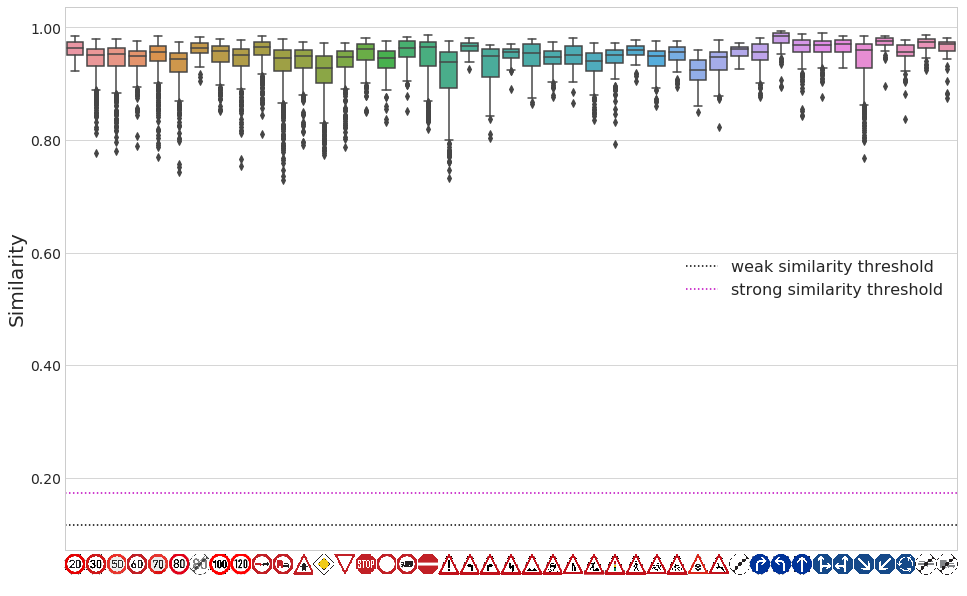
\includegraphics[width=1.0\linewidth]{imgs/Visual_vocab_traffic_signs_similarity_with_representative_vecs.eps}
    \caption{Boxplots depicting the cosine similarities between the representative (mean) vector for each traffic sign class and all individual vector samples it has been created from.}
    \label{fig:visual_vocab_traffic_signs_similarity_with_representative_vecs}
    \vspace{-0.4cm}
\end{figure}

To generate our vocabulary vectors, we cut off the classification layer with softmax activation and use the previous \num{300}-dimensional, fully connected layer as output.
With this simple adaptation, the \ac{CNN} produces a \num{300}-dimensional vector as output for each image fed into the network. 
To generate a representative vector for each class of traffic signs, several approaches are conceivable, including (weighted) mean and median by dimension or regarding whole vectors.
In this work, we choose the simple mean to create this representative from several examples.
To select the example vectors to calculate the representative mean vector from, we select only instances for which the network produces correct classification predictions alongside high confidence values from the test subset of the \ac{GTSRB} data set.
The great majority of examples even satisfies the restriction of \SI{100}{\percent} confidence, hence we use that strict confidence value to avoid including examples the network is doubtful about, which might deteriorate the properties of the representative vector. 
This procedure leads to a representative vector that \enquote{points} to the center of mass of all (high confidence) vectors of each class of traffic signs.
However, we still need to confirm that these representative vectors fulfill the properties they have been constructed for, namely sharing a high cosine similarity with all individual samples from the respective traffic sign class.
Figure~\ref{fig:visual_vocab_traffic_signs_similarity_with_representative_vecs} shows the cosine similarity between each vocabulary vector encoding one traffic sign class with all individual vector samples it has been created from.
As expected, we observe high similarity values close to the maximum value of \num{1} and way above both, weak and strong, similarity thresholds for \num{300}-dimensional vectors.

\begin{figure}[t]
    \centering
    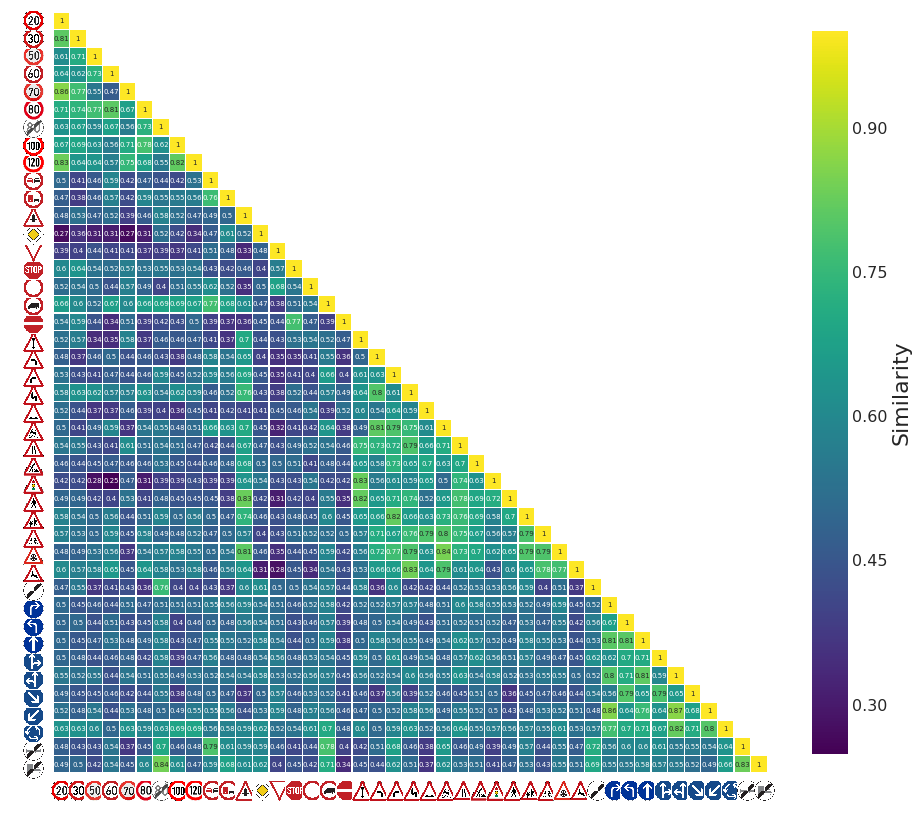
\includegraphics[width=1.0\linewidth]{imgs/visual_vocab_traffic_signs_internal_similarities.eps}
    \caption{Pairwise similarities between representative vectors encoding traffic signs in a visual vector vocabulary.}
    \label{fig:visual_vocab_traffic_signs_internal_similarities}
    \vspace{-0.5cm}
\end{figure}

Furthermore, we expect these representative vectors, which are now our vocabulary vectors encoding the respective traffic signs, to resemble the visual similarity structure of the image classes. 
To confirm this inherent similarity structure, we calculate pairwise similarities between all vectors in the vocabulary, which are visualized in Fig.~\ref{fig:visual_vocab_traffic_signs_internal_similarities}.
We observe similarities in groups of signs indicated by green areas in the heat map visualization.
Most prominent are the high similarities in three groups of traffic signs forming green triangles in the heat map.
These groups are round signs with red borders (top left corner), triangular warning signs with red borders (middle right) and blue signs indicating driving directions (close to bottom right).
Furthermore, several signs stand out particularly: The traffic sign indicating \enquote{Priority ahead}, which is a red triangle just like any warning signs, indeed shows high similarity to all warning signs.
Similarly, the traffic sign indicating no entry for trucks, a red circle with a black truck inside, looks a lot like speed limit signs and indeed shows a high similarity to all speed limit signs.
Consequently, we conclude that it is possible to encode visual similarity with an automatic learning approach using \acp{CNN} to encapsulate the visual features of a given data set into a vocabulary of semantic vectors.

\subsubsection{Traffic participants}%
\label{ssubsec:traffic_participants}

To encode the object categories for traffic participants \emph{Bicycle}, \emph{Car}, \emph{Motorcycle}, \emph{Pedestrian}, \emph{Truck} necessary to properly represent dynamic automotive scenes in visual vectors, we employ an approach similar to the one used for traffic signs.
We adopt a general purpose image data set, the Imagenet data set \parencite{Deng2009}, which includes suitable categories for all of these classes.
As an additional advantage, Imagenet is a widely used data set, so there already exists a number of successful classification networks, which can be adapted for our purposes.
Concretely, we employ the following categories as they appear visually most suitable for the objects categories we want to encode:
We use the original labels 'SAFETY BICYCLE' to learn visual vectors for \emph{Bicycle}, 'USED CAR' for \emph{Car} (other car categories include ambulances and many sports / racing cars), 'MOTORCYCLE', 'PERSON' for \emph{Pedestrian} (since there is no special category for people in the vicinity of roads) and 'TRUCK'.
For each category, there are at least \num{1200} images available in the data set.


\begin{figure}[t]
    \centering
    \resizebox{.95\textwidth}{!}{%
        \subfloat[\label{subfig:visual_vocab_traffic_participants_similarity_with_representative_vecs}]{%
            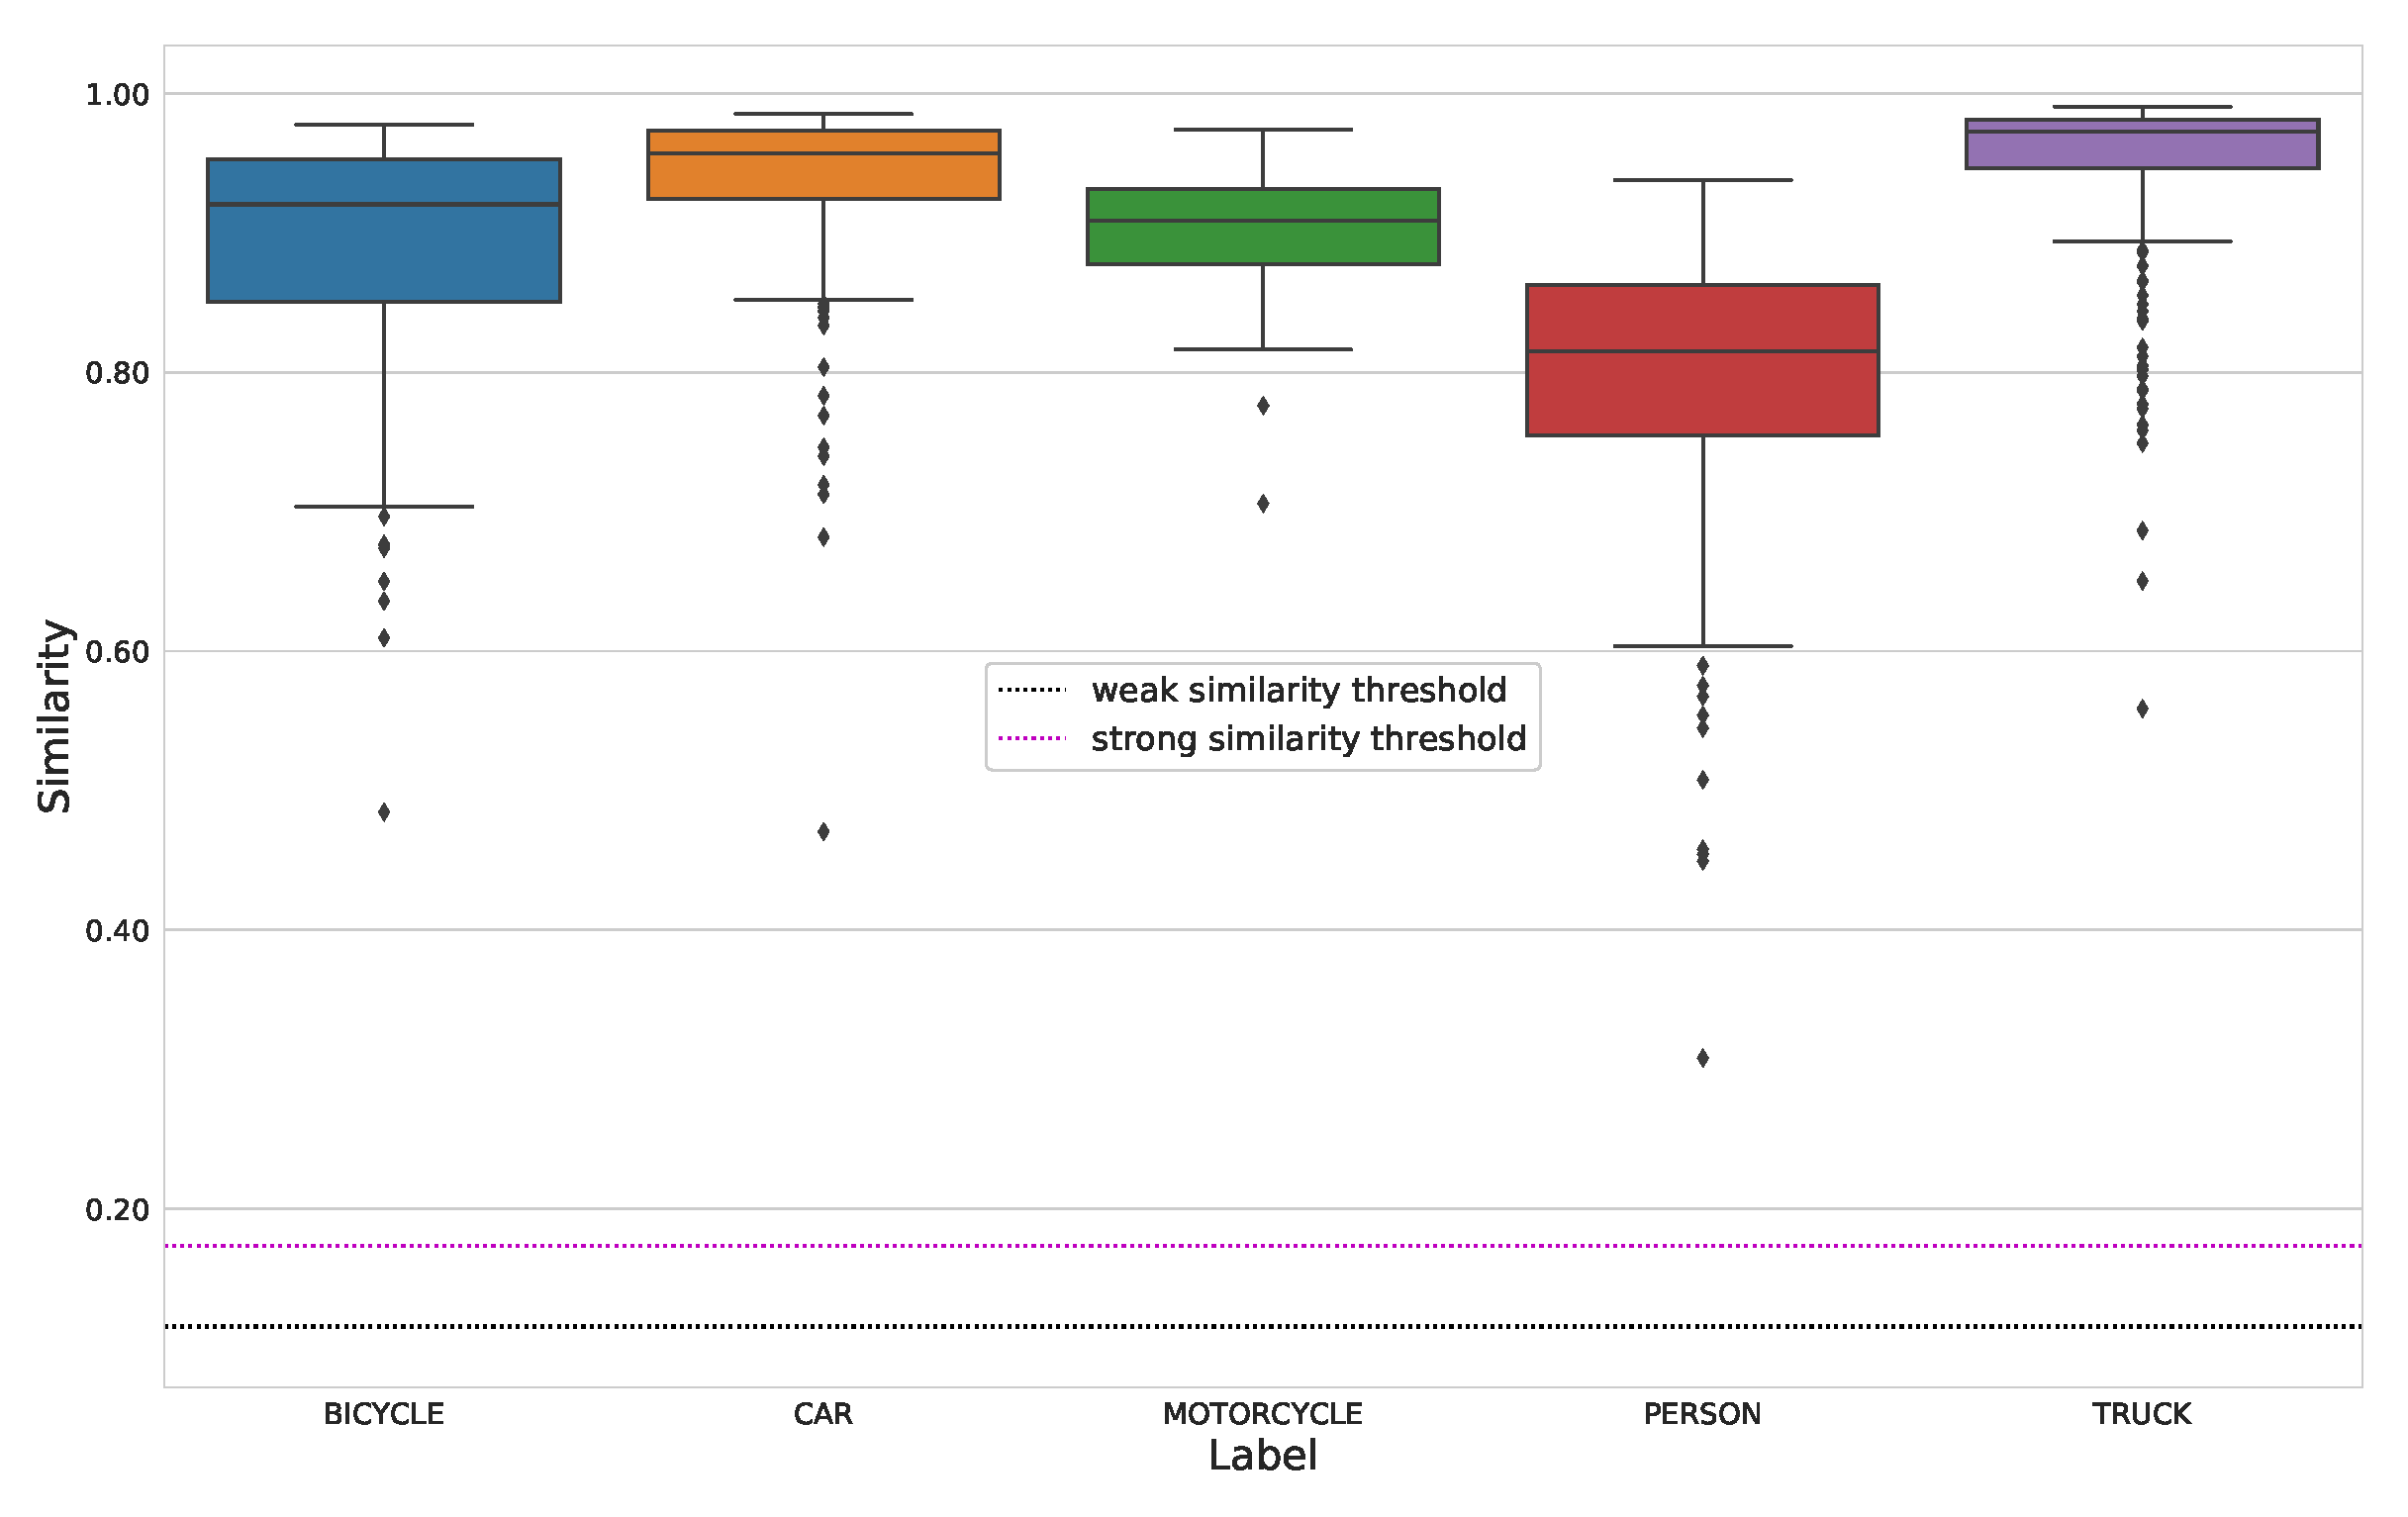
\includegraphics[height=3.5cm]{imgs/Visual_vocab_traffic_participants_similarity_with_representative_vecs.eps}
        }
        \subfloat[\label{subfig:visual_vocab_traffic_participants_internal_similarities}]{%
            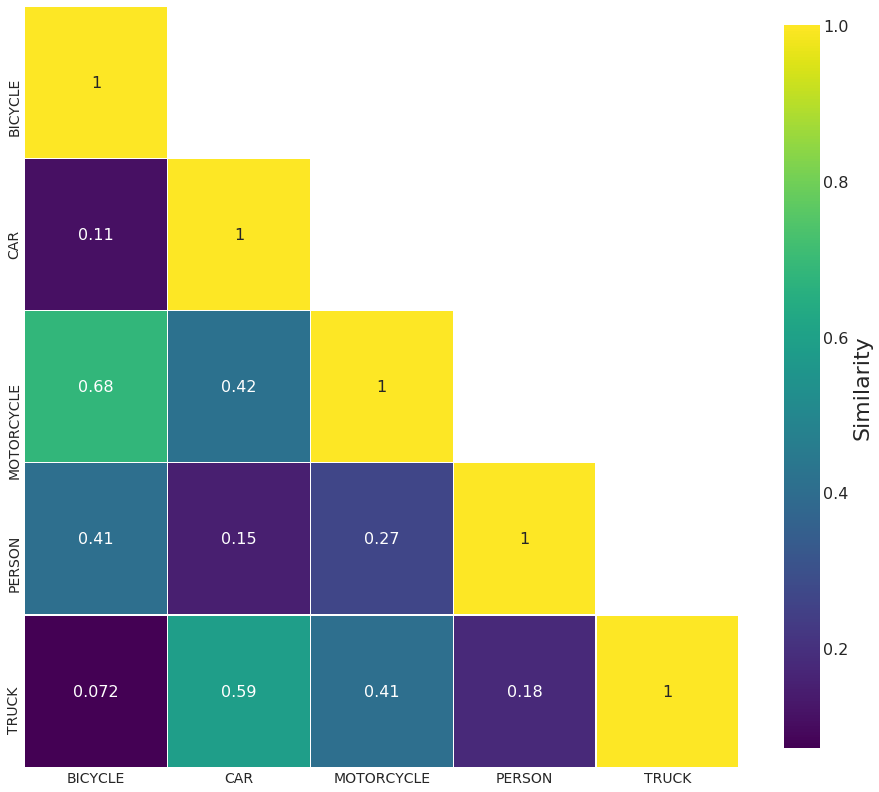
\includegraphics[height=3.5cm]{imgs/visual_vocab_traffic_participants_internal_similarities.eps}
        }
    }
    \caption{Similarity plots for the visual vocabulary vectors representing traffic participants.~\protect\subref{subfig:visual_vocab_traffic_participants_similarity_with_representative_vecs} Boxplots depicting the cosine similarities between the representative (mean) vector for each traffic participant class and all individual vector samples it has been created from.~\protect\subref{subfig:visual_vocab_traffic_participants_internal_similarities} Pairwise similarities between representative
    vectors encoding traffic participants in our visual vector vocabulary.}
    \label{fig:visual_vocab_traffic_participants}
    \vspace{-0.6cm}
\end{figure}

While there is a number of state-of-the-art classification networks available achieving good results on the Imagenet data set, we are looking for a network with only moderately complex structure for the sake of implementation simplicity and ease of adaptation, while performance is of secondary priority.
VGG19 is a deep \acf{CNN} proposed by \textcite{Simonyan2014} with a decent performance on the Imagenet data set (top 1 performance \SI{73}{\percent} and top 5 performance \SI{91}{\percent}) and a comparatively simple layer by layer architecture that allows easy extraction of results from intermediate layers.
Our goal is to train a variant of the VGG19 network on these \num{5} classes and extract feature vectors of an intermediate layer to use them as vocabulary vectors.
Therefore, we adapt the original network architecture in the following way:
We cut off the last two fully connected layers as well as the classification layer and replace them with a fully connected, \num{300}-dimensional layer and a \num{5} dimensional classification layer. 
We train the modified network using the categorical cross entropy loss and \enquote{standard} stochastic gradient descent optimization.

Table~\ref{tab:traffic_participant_visual_accuracy} depicts the classification performance of our adapted VGG19 network for the \num{5} selected traffic participant categories.
Except for the \enquote{MOTORCYCLE} class, the network achieves decent classification results above \SI{75}{\percent}, which is sufficient for our purposes.
Similar to the creation of the visual vocabulary for traffic signs, we calculate the mean of vectors produced by the second to last of the network's layers when making correct predictions with \SI{100}{\percent} confidence.
Even for the \enquote{MOTORCYCLE} class, there are at least \num{139} of such vectors available, whereas for all other classes, we have at least \num{200} of such vectors.
To confirm that the vocabulary vectors created in this fashion are visually representative enough for each class, we calculate the cosine similarity between the vocabulary vectors and all vector samples they have been created from.
Figure~\ref{subfig:visual_vocab_traffic_participants_similarity_with_representative_vecs} visualizes these similarities as box plots.
Similar to the traffic sign vocabulary, we observe high similarity values close to the maximum value of \num{1} and way above both, weak and strong, similarity thresholds for \num{300}-dimensional vectors.
We also calculated pairwise similarities between all vocabulary vectors encoding traffic participants, which are visualized in Fig.~\ref{subfig:visual_vocab_traffic_participants_internal_similarities}.
As expected, visually similar classes such as \enquote{BICYCLE} and \enquote{MOTORCYCLE} as well as \enquote{CAR} and \enquote{TRUCK} share relatively high cosine similarities.
Less similar, but still significantly higher than the similarity thresholds, are traffic participants sharing the visual features of persons such as \enquote{PERSON} and \enquote{BICYCLE}, \enquote{PERSON} and \enquote{MOTORCYCLE} as well as \enquote{BICYCLE} and \enquote{MOTORCYCLE}.
All other pairs have similarity values in the order of magnitude or below the similarity thresholds and are therefore considered dissimilar while we do not attach the greatest importance to the actual (low) numbers.
Consequently, we can conclude, that we are able to encode visual similarity of traffic signs as well as traffic participants in a visual vector vocabulary.
\begin{center}
	\begin{tabular}{|c|c|c|c|c|c|}
		\hline
		 & BICYCLE & CAR & MOTORCYCLE & PERSON & TRUCK\\ \hline
        Classification accuracy & \SI{94.3}{\percent} & \SI{76}{\percent} & \SI{55}{\percent} & \SI{82.6}{\percent}& \SI{99}{\percent}\\ \hline
	\end{tabular}
	\captionof{table}{Classification accuracy of the adapted VGG19 network for our selected \num{5} classes of traffic participants.}
	\label{tab:traffic_participant_visual_accuracy}
\end{center}

\subsection{Semantic vocabularies}%
\label{subsec:semantic_vocabularies}

\begin{figure}[t]
    \centering
    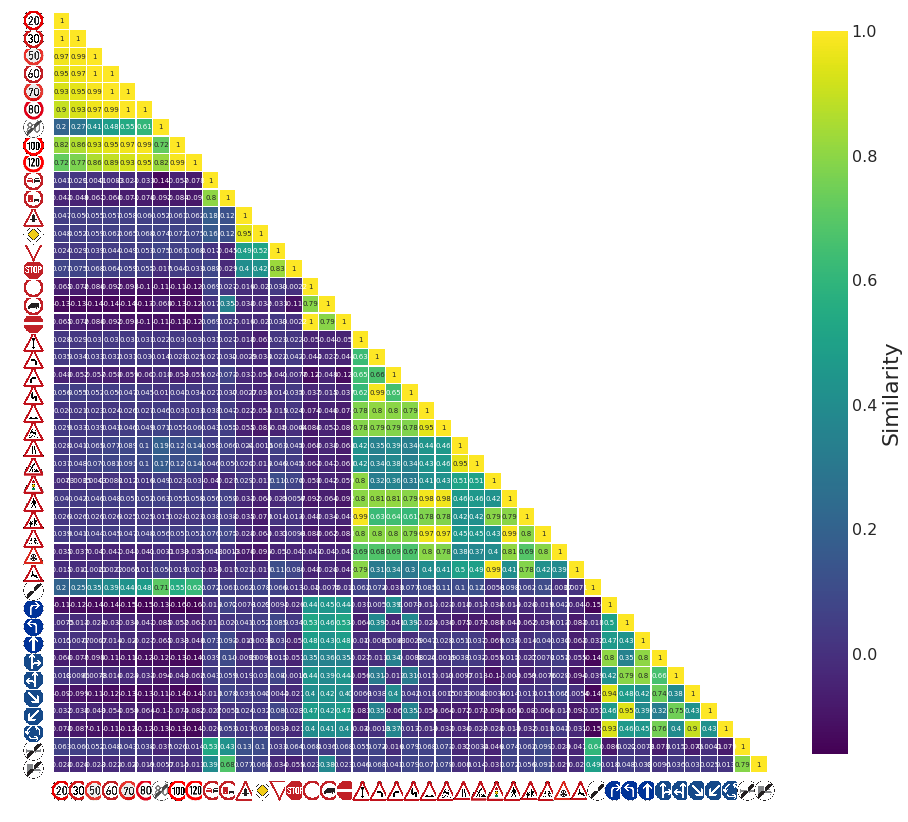
\includegraphics[width=1.\linewidth]{imgs/semantic_vocab_traffic_signs_internal_similarities.eps}
    \caption{Pairwise similarities between representative vectors encoding traffic signs in a manually designed semantic vector vocabulary.}
    \label{fig:semantic_vocab_traffic_signs_internal_similarities}
\end{figure}
In this section, we go one step further and try to encapsulate semantic similarity structures within a vector vocabulary.
As discussed in section~\ref{ssubsec:semantic_similarity}, semantic similarity as a concept is comparatively intuitive for traffic signs and less obvious for other objects, such as traffic participants.
Furthermore, we also highlighted in that section that semantic similarity in other domains such as language modeling typically unfolds through proximity, i.e., that similar words appear in similar contexts or proximity within the text.
While this could give a hint towards what kind of learning procedure could be used to automatically generate a semantic vocabulary in automotive context, availability of suitable data sets is rather limited.
Analogously to the visual vocabulary, we consider the encoding of traffic signs and traffic participants separately in this section as well. 

\subsubsection{Traffic signs}%
\label{ssubsec:traffic_signs}

Our goal is to encode the meaning of traffic signs, i.e., the driving instruction or traffic rule they indicate to the driver in a semantic vector vocabulary.
As with visual similarity, this goal could be achieved by either manually engineering the similarity structure through the \ac{VSA}'s algebraic operations from randomly chosen atomic vectors or through some automated learning approach.
If we were to learn this similarity structure automatically, there are two possible approaches. 
Similar to word embedding algorithms for language, we could either learn the meaning of traffic signs explicitly from a large  corpus of text that describes traffic signs and their meanings in context.
Alternatively, we could try to learn the semantic meaning of traffic signs implicitly from many dynamic driving situations.
Unfortunately, there are no suitable data sets available for either of the aforementioned learning approaches.
Additionally, an implementation of the latter, implicit learning approach would be quite complex, as it would require additional steps to extract structural understanding from the driving scene, which would be necessary for the vocabulary generation system to create suitable vectors.
To our knowledge, such a system does not exist.
Consequently, the only remaining option is to manually design the desired similarity structure as described in section~\ref{subsec:basic_random_vocabularies}.

To encode the semantic meaning of traffic signs, we choose atomic vectors for the basic building blocks of the representation at random and create semantic structure by employing the algebraic operations of the \ac{SPA}.
We apply the role-filler pair approach described in section~\ref{subsec:encoding_struct}.
We randomly choose vectors for the roles \textbf{TYPE} and \textbf{MEANING} encoding the type and the meaning of a particular traffic sign.
For some traffic signs, we need an additional role \textbf{REASON} giving further information to the vocabulary vector in order to distinguish similar traffic signs from one another.
As potential filler vectors for the \textbf{TYPE} role, we choose random vectors representing the following traffic sign classes included in the \ac{GTSRB}: \textbf{LIMIT}, \textbf{PASSING}, \textbf{PRIORITY}, \textbf{DIRECTION} and \textbf{ATTENTION}.
Similarly, we create filler vectors for the \textbf{MEANING} role like \textbf{RIGHTOFWAY}, \textbf{GIVEWAY}, \textbf{SLOW}, \textbf{PREPARETOSTOP}, \textbf{CONCENTRATE}, \textbf{LEFT}, \textbf{RIGHT}, \textbf{STRAIGHT}, \textbf{OVERTAKING}.
Finally, we create filler vectors for the \textbf{REASON} role indicating the reason for increased attention or other additional information such as \textbf{PEDESTRIANS}, \textbf{CHILDREN} or \textbf{SLIPPERYROAD}, \textbf{ROADWORKS}.
Given these role and filler vectors, we generate semantic vocabulary vectors encoding the meaning of traffic signs in the following way

\begin{equation}
    \label{eq:semantic_vocab_traffic_signs}
    \mathbf{SIGN} = \mathbf{TYPE} \varoast \mathbf{FT} + \mathbf{MEANING} \varoast \left( \sum\limits_{i=0}^{n} \beta_{i} \cdot  \mathbf{FM}_{i}  \right) + \gamma \cdot \mathbf{REASON} \varoast \mathbf{FR}, 
\end{equation}
where \textbf{FT}, $\mathbf{FM}_{i}$ for $i = 0, \ldots, n$ and \textbf{FR} are placeholders for the filler vectors and $\beta_{i} \in \mathbb{R} $ for $i = 0, \ldots, n$ and $\gamma \in \mathbb{R} $ are weighting factors.
In case, the additional \textbf{REASON} role is not needed for a particular traffic sign, the corresponding weight factor $\gamma$ is set to \num{0}.
For instance, the vocabulary vector encoding the traffic sign indicating danger is calculated as

\begin{equation}
\label{eq:semantic_vocab_traffic_sign_example}
\mathbf{DANGER} = \mathbf{TYPE} \varoast \mathbf{ATTENTION} + \mathbf{MEANING} \varoast  \left(\mathbf{SLOW} + \mathbf{PREPARETOSTOP}\right).
\end{equation}

Traffic signs indicating speed limits form somewhat of a special case, as we want to encode them in such a way, that signs indicating lower speed limits are more similar to one another than to signs indicating higher speed limits.
To achieve that, we need to encode numerical values that are closer to one another more similarly than numerical values with larger intervals.
Here, we employ a very simple encoding scheme using the function 
\begin{equation}
\label{eq:cosin_vec_func}
\abb{\varphi}{\mathbb{R}}{\mathbb{R}^{D}}{x}{\left(\sin(x), \cos(x), 0, \ldots, 0\right)}.
\end{equation}
In other words, we create a vector representing the numerical value of the speed limit by setting the first two dimensions to $\sin(x)$ and $\cos(x)$ for the encoded numerical value $x \in [0,\frac{\pi}{2}]$ and all other entries to \num{0} (note that we will discuss other, more complex approaches to encode numerical values in vectors in section~\ref{subsec:different_vector_representations_for_numerical_values}).
We use \SI[per-mode=symbol]{200}{\kilo\meter\per\hour} as general speed limit, i.e., we map all speed limit values between \num{0} and \num{200} to the interval $\left[0, \frac{\pi}{2}\right]$ with \SI[per-mode=symbol]{200}{\kilo\meter\per\hour} $\equiv \frac{\pi}{2}$.

Figure~\ref{fig:semantic_vocab_traffic_signs_internal_similarities} shows the pairwise similarities between the manually designed semantic vectors encoding traffic signs in the \ac{GTSRB} created in the aforementioned fashion.
As expected, we see a highly structured area in the top left corner, the speed limit signs.
The other groups of signs (overtaking, priority, warning and direction) are also visible as triangles on the right hand side.
All non-related entities have low similarities of less than \num{0.1}.
Brighter spots in the large dark area to the left represent similarities across sign groups, especially, for signs related to trucks and curves or bends.
Consequently, we were successful in manually designing a vocabulary encapsulating semantic similarity of traffic signs as an alternative to the visual vocabulary created in section~\ref{subsec:visual_vocabularies}.

\subsubsection{Traffic participants}%
\label{ssubsec:traffic_participants}

\begin{figure}[t]
    \centering
    \resizebox{.9\textwidth}{!}{%
        \subfloat[\label{subfig:semantic_vocab_traffic_participants_word2vec_internal_similarities}]{%
            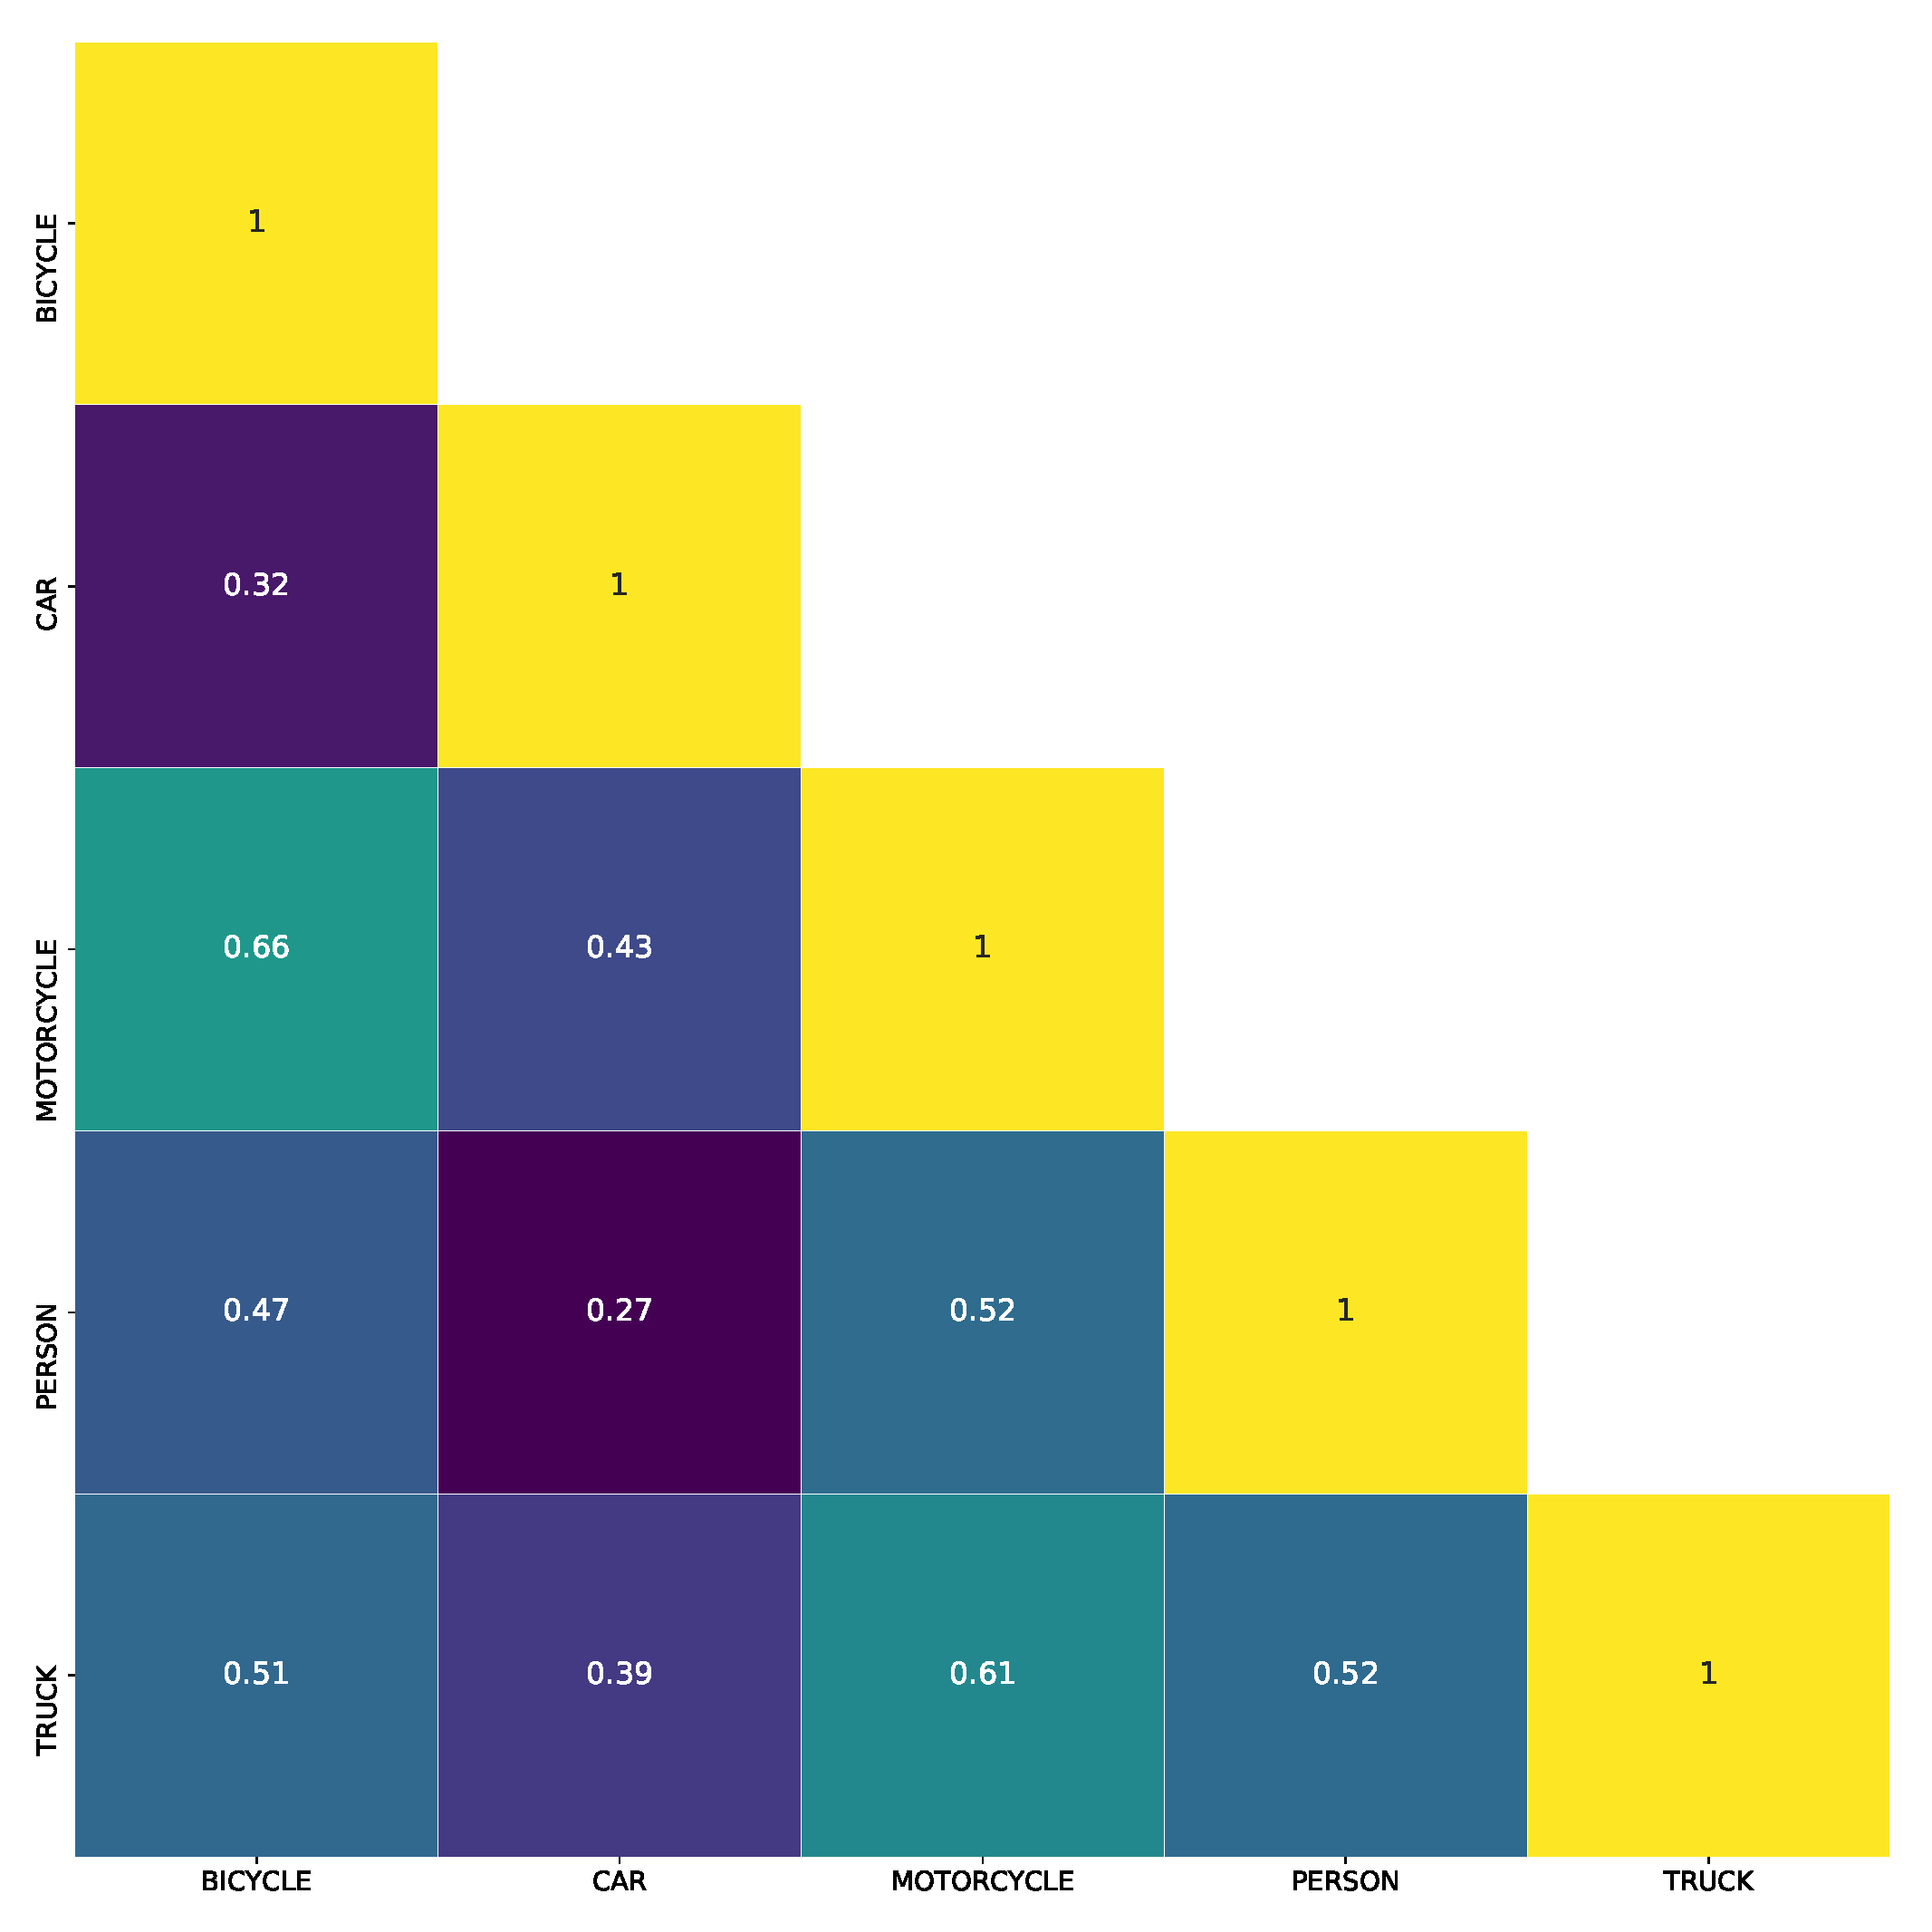
\includegraphics[height=3cm]{imgs/semantic_vocab_traffic_participants_word2vec_internal_similarities.eps}
        }
        \subfloat[\label{subfig:semantic_vocab_traffic_participants_manual_internal_similarities}]{%
            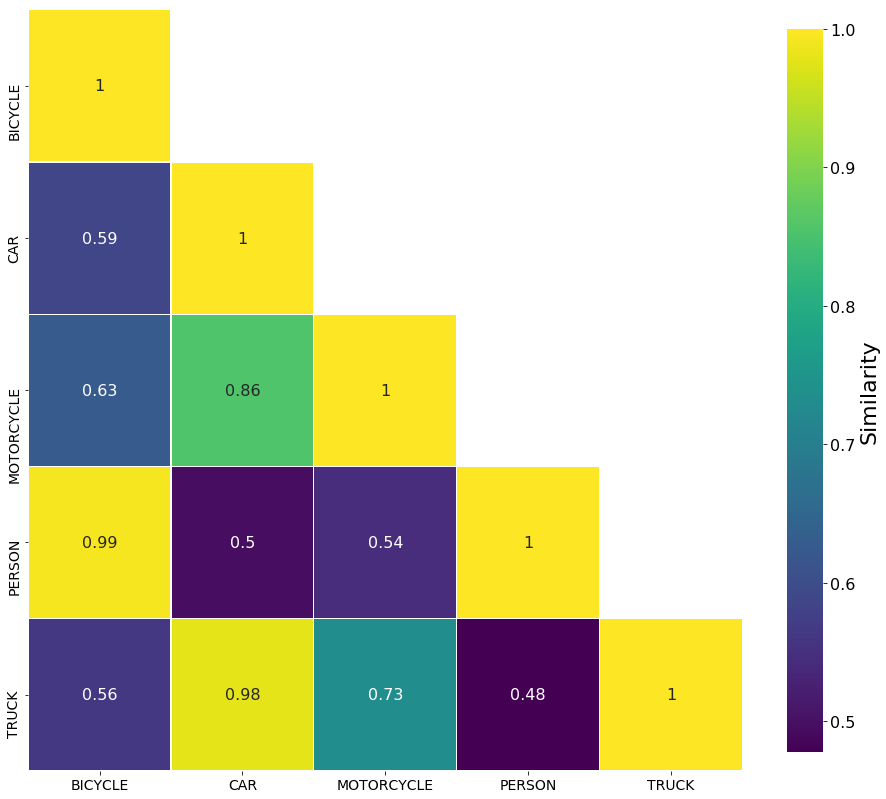
\includegraphics[height=3cm]{imgs/semantic_vocab_traffic_participants_manual_internal_similarities.eps}
        }
    }
    \caption{Pairwise similarities between representative vectors encoding traffic participants in a semantic vector vocabulary.~\protect\subref{subfig:semantic_vocab_traffic_participants_word2vec_internal_similarities} Learned with word2vec~\protect\subref{subfig:semantic_vocab_traffic_participants_manual_internal_similarities} manually designed.}
    \label{fig:semantic_vocab_traffic_participants_internal_similarities}
\end{figure}

As discussed in section~\ref{subsec:what_types_of_data_to_encode_}, semantic similarity for traffic participants is hard to capture intuitively.
We concluded that the general meaning of traffic participants is highly context-dependent, which in turn can only be learned from dynamic driving data or from a text corpus describing traffic situations.
However, such data sets are either not available or do not even exist.
Hence, as a first step towards the goal of encoding semantic similarity, we will therefore encapsulate the similarity between the five classes of traffic participants already discussed in section~\ref{subsec:visual_vocabularies}, namely \emph{Bicycle}, \emph{Car}, \emph{Motorcycle}, \emph{Pedestrian}, \emph{Truck}.
Here, we employ two different approaches: an automated learning approach making use of the well-established word embedding of the word2vec algorithm \parencite{Mikolov2013} trained on the Google News data set and, similar to the semantic vocabulary of traffic signs, manual design, which is only possible due to the small size of our vocabulary.
Word2vec is an unsupervised learning approach generating a word embedding, i.e., vectors representing every word encountered in the training text, where words that appear in similar context, i.e., close proximity within the text, are mapped to similar vectors. 
For our purposes, we simply extract the (\num{300}-dimensional) vectors representing the objects of interest (traffic participants) from the learned vocabulary.
The manually designed semantic vocabulary is generated similarly to the aforementioned vocabulary of traffic signs using the \ac{SPA}'s algebraic operation and the role-filler-pairs approach based on two key properties, which give good yet simple descriptions of the traffic participant's semantic properties: speed and vulnerability represented by randomly chosen atomic vectors \textbf{SPEED} and \textbf{VULNERABILITY}.
Hence, we encode the five classes of traffic participants through

\begin{equation}
\label{eq:semantic_vocab_traffic_participants}
\mathbf{PARTICIPANT} = \mathbf{SPEED} \varoast \varphi(s) + \mathbf{VULNERABILITY} \varoast \varphi(v),
\end{equation}
using the encoding function $\varphi$ from Equation~\eqref{eq:cosin_vec_func}.

Figure~\ref{fig:semantic_vocab_traffic_participants_internal_similarities} depicts the pairwise similarities of both, the semantic vocabulary using word2vec vectors (Fig.~\ref{subfig:semantic_vocab_traffic_participants_word2vec_internal_similarities}) and the manually designed vocabulary vectors (Fig.~\ref{subfig:semantic_vocab_traffic_participants_manual_internal_similarities}).
We observe that the pre-trained word vectors from word2vec are not entirely successful to capture the kind of semantic similarity we are interested in.
While vectors are similar to each other, the individual similarities do not always match our human understanding, especially when considering an automotive context.
For instance, the vector encoding \emph{person} is significantly more similar to the one representing \emph{truck} than to the one representing \emph{car} 
Furthermore, \emph{car} is the traffic participant least similar to \emph{truck}. 

For the manually designed vocabulary (Fig. \ref{subfig:semantic_vocab_traffic_participants_manual_internal_similarities}), results are more convincing.
We are able to achieve a higher similarity between vectors encoding \emph{car} and \emph{truck} as well as \emph{bicycle} and \emph{person} with lower similarities between \emph{person} and \emph{truck} as well as \emph{bicycle} and \emph{truck}.
This vocabulary is also not an ideal representation but gets much closer to the desired semantic structure between these entities in an automotive context. 

\subsection{Visual-semantic vocabularies}%
\label{subsec:visual_semantic_vocabularies}
 
After having created vector vocabularies encoding visual (section~\ref{subsec:visual_vocabularies}) and semantic similarity (section~\ref{subsec:semantic_vocabularies}) structures, we aim to generate a vector vocabulary, which combines both aforementioned similarities in one comprehensive vocabulary.
The idea is that for high or low similarity in both, visual and semantic domain we want the resulting vectors to preserve or even increase that similarity structure.
For a diverging similarity in the two domains, the fusion process should somewhat dilute the two extremes resulting in vectors with medium similarity.
Contrary to other visual-semantic fusion methods, these properties can be achieved employing again the algebraic operations of the \ac{SPA} and the role-filler-pair approach.
Therefore, we randomly choose two additional role vectors, \textbf{VISUAL} and \textbf{SEMANTIC} and construct the visual-semantic vocabulary vectors as
\begin{equation}
\label{eq:visual_semantic_vocab}
\mathbf{VISUALSEMANTIC} = \mathbf{VISUAL} \varoast \mathbf{V} + \mathbf{SEMANTIC} \varoast \mathbf{S},
\end{equation}
where \textbf{V} and \textbf{S} are placeholders for the visual and semantic vocabulary vectors to be fused.
Given the mathematical properties of the \ac{SPA}'s algebraic operations (cf.\ chapter~\ref{chap:introduction_to_vsas}), this fusion procedure guarantees that for two similar vectors in either of the input domains, the resulting visual-semantic vectors will preserve that similarity.

\subsubsection{Traffic signs}%
\label{ssubsec:traffic_signs}

\begin{figure}[t]
    \centering
    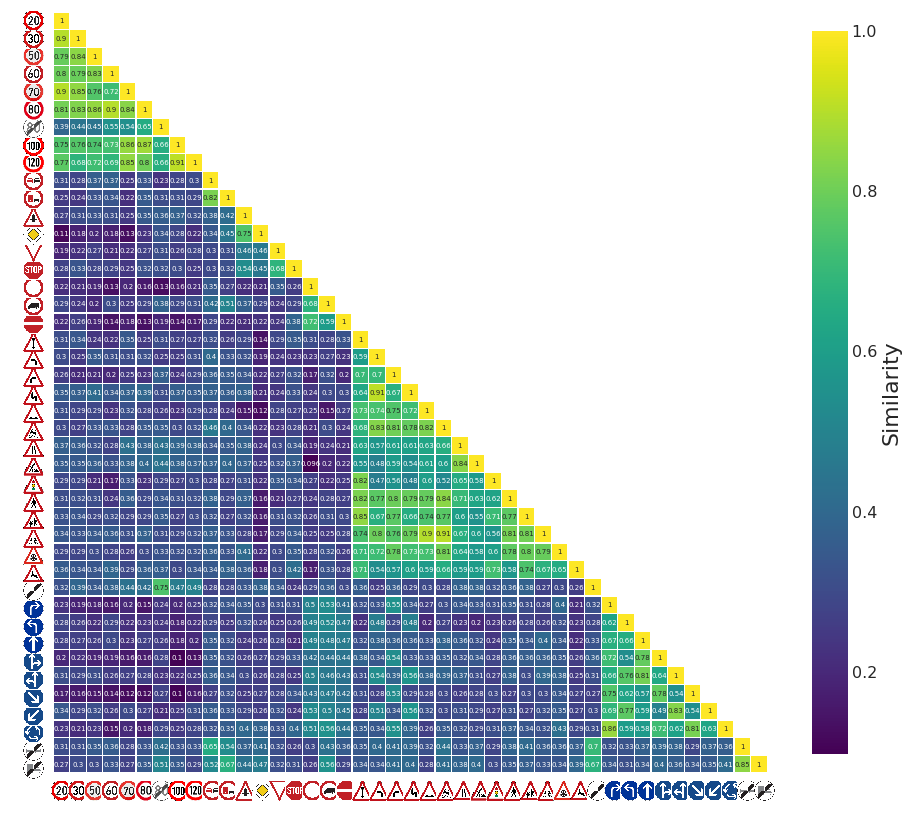
\includegraphics[width=1.0\linewidth]{imgs/visual_semantic_vocab_traffic_signs_internal_similarities.eps}
    \caption{Pairwise similarities between vectors encoding traffic signs in a visual-semantic vocabulary.}
    \label{fig:visual_semantic_vocab_traffic_signs_internal_similarities}
\end{figure}

Figure~\ref{fig:visual_semantic_vocab_traffic_signs_internal_similarities} shows the pairwise similarities of the visual-semantic vocabulary vectors representing traffic signs.
We observe that opposite similarities from the input domains are smoothed out through the convolution-based fusion process.
For instance, the strong visual similarity between the traffic sign indicating \enquote{Priority ahead} and all attention signs (triangular shape, red border, black symbol in the middle), which has been clearly visible in Fig.~\ref{fig:visual_vocab_traffic_signs_internal_similarities}, does not correspond to a large semantic similarity and was canceled during the fusion procedure.
The same holds true for the clearing signs as well as for the similarities between signs indicating \enquote{No entry trucks} and \enquote{roundabout} and the speed limits.
On the other hand, for those traffic signs with high semantic similarity such as between signs indicating overtaking rules for trucks and the sign indicating no entry for trucks, this similarity is preserved in the joint visual-semantic vocabulary. 
Particularly for the speed limits, we observe that a high similarity in both domains translates into a high joint similarity, whereas in other cases, the manually designed semantic similarity is partly \enquote{overwritten} with the visual information.
In general, many signs from different groups with very low semantic similarity (the dark blue block in the bottom left of Fig.~\ref{fig:visual_semantic_vocab_traffic_signs_internal_similarities}) are increased by the visual part. 

\subsubsection{Traffic participants}%
\label{ssubsec:traffic_participants}

\begin{figure}[t]
    \centering
    \resizebox{.9\textwidth}{!}{%
        \subfloat[\label{subfig:visual_semantic_vocab_traffic_participants_word2vec_internal_similarities}]{%
            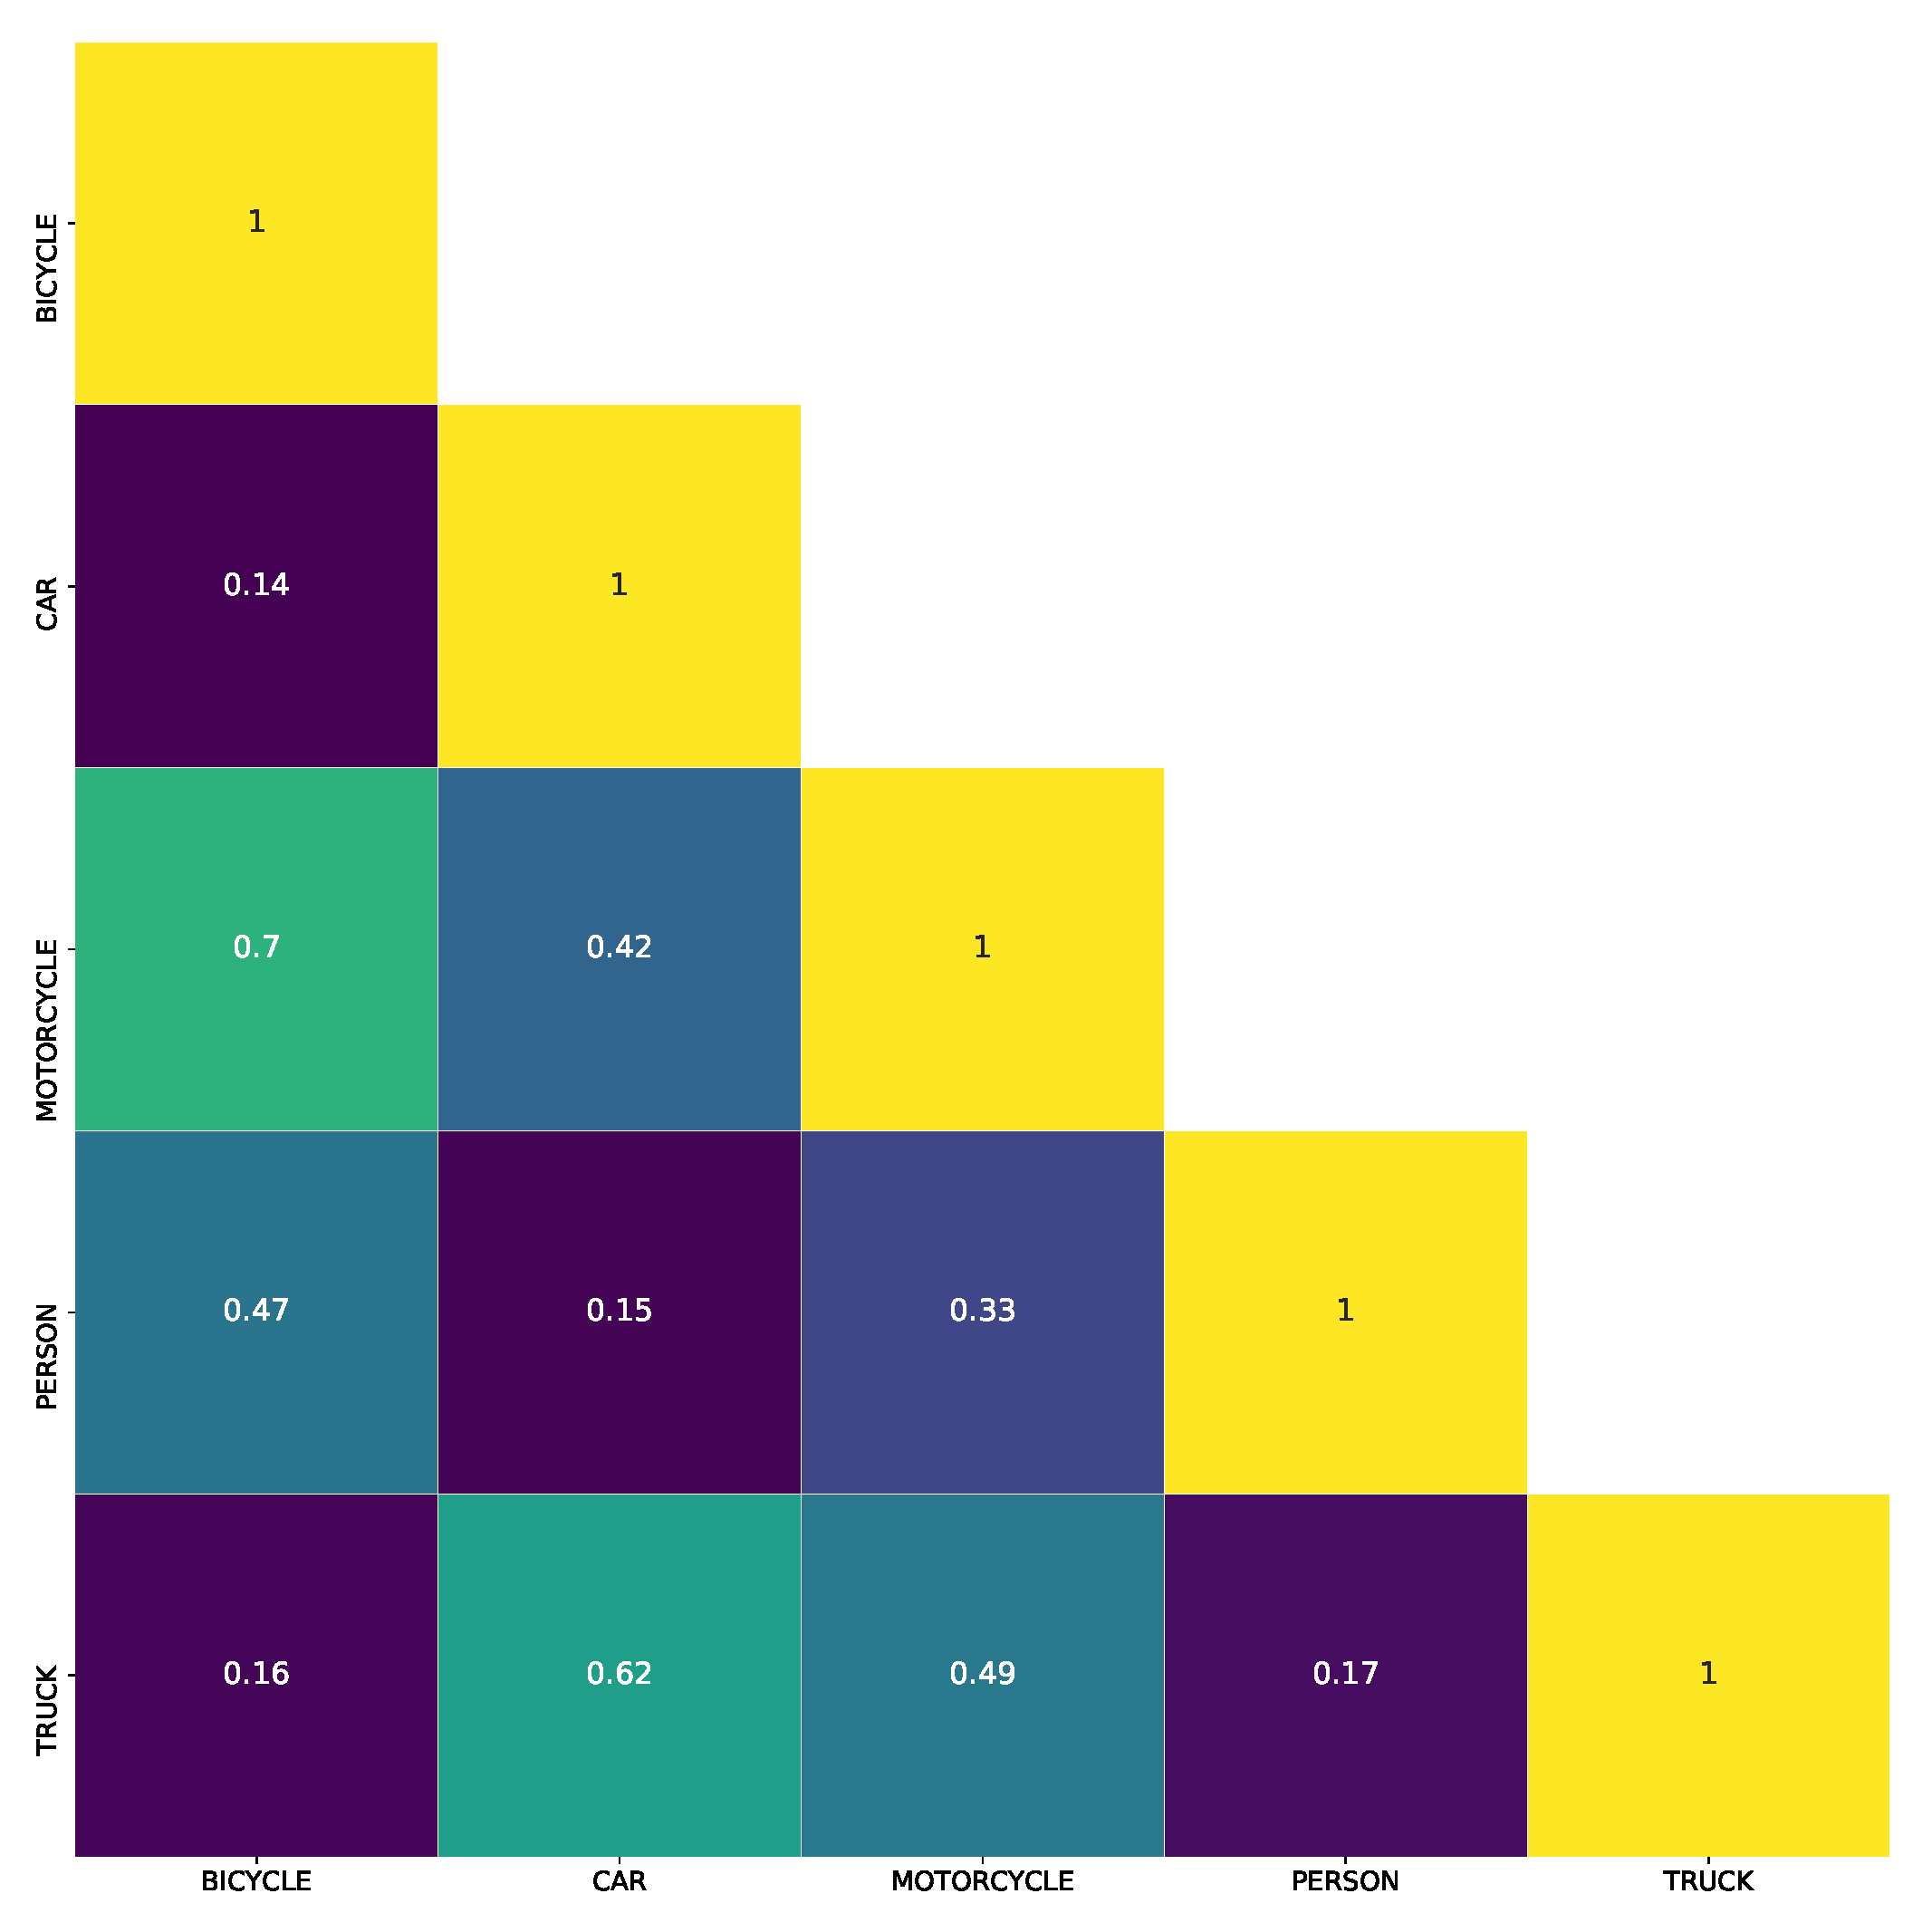
\includegraphics[height=3cm]{imgs/visual_semantic_vocab_traffic_participants_word2vec_internal_similarities.eps}
        }
        \subfloat[\label{subfig:visual_semantic_vocab_traffic_participants_manual_internal_similarities}]{%
            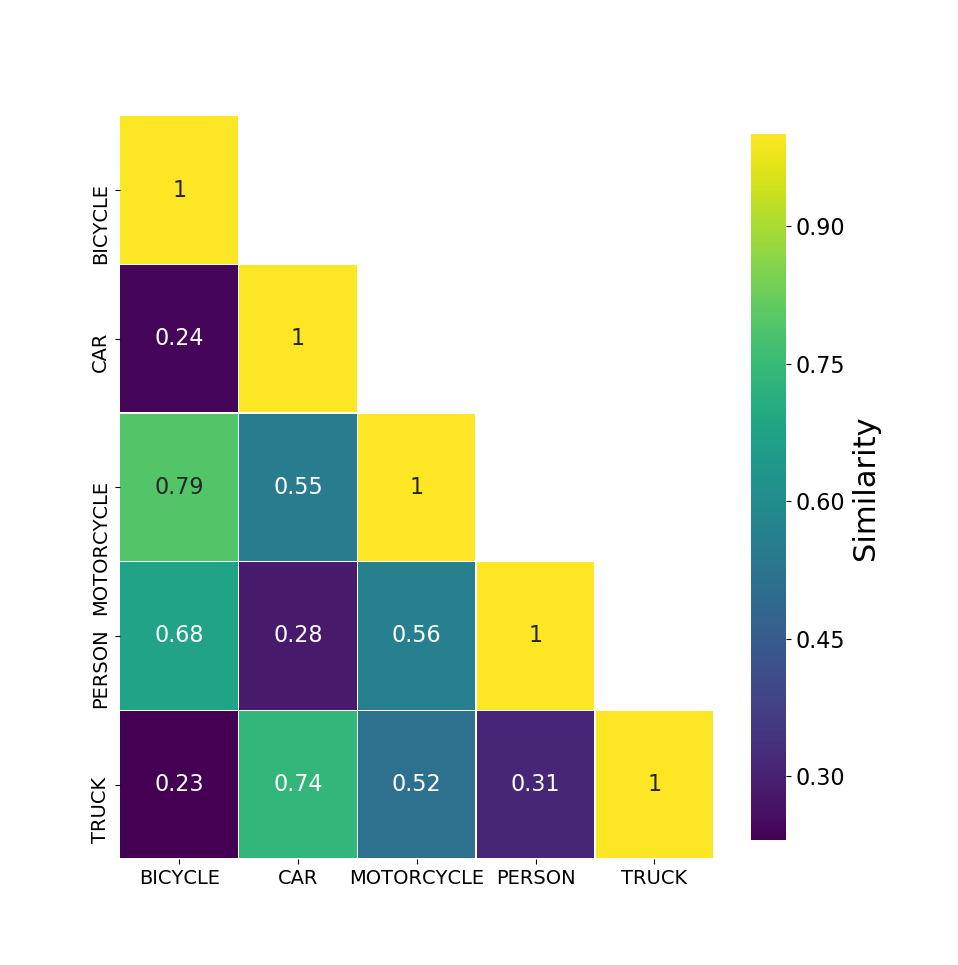
\includegraphics[height=3cm]{imgs/visual_semantic_vocab_traffic_participants_manual_internal_similarities.eps}
        }
    }
    \caption{Pairwise similarities between vocabulary vectors encoding traffic participants in a visual-semantic vocabulary, where the semantic part is~\protect\subref{subfig:semantic_vocab_traffic_participants_word2vec_internal_similarities} learned with word2vec~\protect\subref{subfig:semantic_vocab_traffic_participants_manual_internal_similarities} manually designed.}
    \label{fig:visual_semantic_vocab_traffic_participants_internal_similarities}
\end{figure}

In section~\ref{subsec:semantic_vocabularies}, we created two semantic vocabularies, which have been learned with word2vec and manually designed.
Figure~\ref{fig:visual_semantic_vocab_traffic_participants_internal_similarities} depicts the pairwise similarities of two visual-semantic vocabularies, where the two different vocabularies from section~\ref{subsec:semantic_vocabularies} are used for the semantic part.
We observe fusion results similar to those for the visual-semantic traffic sign vocabulary, where opposite similarities from the input domains are smoothed out through the convolution-based fusion process while differences in semantic structure between the two methods remain visible in the complete vocabulary.
Consequently, the visual-semantic encoding based on manually designed semantics appear to be a convincing vector representation for the similarity structure expected for traffic participants in an automotive context.

\subsection{Summary on vocabularies}%
\label{subsec:summary_on_vocabularies}

In this section, we investigated several options of generating a suitable vector vocabulary for entities of interest in an automotive context.
We have shown a way of learning a visual structure for two classes of categories appearing in an automotive context, namely traffic signs and traffic participants using \acp{CNN}.
Furthermore, we were able to create a learned semantic vocabulary for traffic participants, but not traffic signs due to lack of suitable training data sets.
Hence, we designed the semantic vocabulary for traffic signs manually using the mathematical properties and algebraic operations of the \ac{SPA}.
Furthermore, we also generate an alternative semantic vocabulary for traffic participants as a baseline to compare the learned semantic structure, which has not been adapted to the automotive context, to.
Finally, we successfully generated a visual-semantic vocabulary encapsulating both, visual and semantic similarity by using the \ac{SPA}'s algebraic operations and the role-filler-pair approach.
This visual-semantic vocabulary appears to represent the expected similarity structure between the entities of interest in automotive context.

It is worth noting however that the manual generation process of the semantic vocabularies, as mentioned in~\ref{subsec:basic_random_vocabularies}, imposes a significant amount of design choices biased by the human engineer.
However, the choice of generating some of the semantic vectors in this context manually is due to the fact that on the one hand, the vocabulary is comparatively small while on the other hand, there are no suitable data sets available to learn the desired semantic structure from.
Furthermore, the described procedure to fuse visual and semantic similarities into one coherent vocabulary is only one of several available options.
It would have also been possible to try to automatically learn such a fusion process by projecting the visual vocabulary to the semantic one by combining visual properties and language descriptions like for instance in \textcite{Karpathy2017}.
However, such a learning approach again would require a suitable, sufficiently large data set, which in turn is not available for the entities investigated here.

Finally, the process of generating structured representations from an available vocabulary created with any of the techniques described in this section is independent from the particular vocabulary at hand.
Hence, although it seems intuitive and useful to encode similarities of potential interest to the task to be solved using the vector representation, it remains to be seen, if using a vocabulary encapsulating any form of similarity actually improves task performance.
Furthermore, the choice which similarity structure to use naturally appears to be heavily task-dependent.
Thus, we will investigate the influence of the vocabulary structure on the task performance for the selected task of driving context classification in chapter~\ref{chap:driving_context_classification} by simply evaluating the same models with changing underlying vocabularies.

\section{Representation generation stage}%
\label{sec:representation_generation_stage}

After having created a vector vocabulary suitable for a specific application of interest as shown in section~\ref{sec:preprocessing_stage_generating_a_vocabulary}, we focus our attention in this section to the second stage of the encoding process proposed by \textcite{Gallant2013}, the \emph{representation generation stage}.
This second step is the process of actually generating structured vector representations from a given vocabulary of atomic vectors.
As mentioned by \textcite{Gallant2013}: \enquote{Although the preprocessing and output computation stage can involve significant machine learning, there are reasons for the representation generation stage to \emph{avoid} machine learning}.
Using machine learning in the stage of representation generation means to adjust the representation to the specific set of applications, which restricts them to be used for different, but related sets of problems.
Furthermore, involving learning in the representation generation might slow down the whole system prohibiting practical usage of the representation in application scenarios.
However, in certain situations it could make sense to involve a learning step at the representation generation stage, for example if the system should detect novelties and assign them to new vectors or representations and/or needs to memorize them.

In this work however, we will focus our efforts mainly on representations which are manually designed without involving machine learning models.
Thereby, we aim to generate representations that are general enough to be applied to a variety of different problems with only moderate modifications necessary when being applied to one particular task.
One crucial aspect in the field of automotive scene representation is encoding dynamic data such as positions or velocities, which constitutes a significant part of the situational context.
This context is essential for the representation to capture the semantics of the scene and gather a comprehensive understanding of the situation at hand.
Depending on the application, different requirements on such a representation might be necessary.
For instance, for some applications it might be necessary that the encoded numerical values need to be decoded back out exactly from the representing vector while for others an approximate recovery might be sufficient.
Other tasks might demand for the representational vectors to have unit length independent from the encoded value.
We therefore investigate several possible options of how to encode numerical values in semantic vectors focusing on different aspects of possible requirements.

Encoding numerical values, although an important one, is only one aspect of representing automotive scenes in high-dimensional vectors.
The second crucial aspect of the representation generation stage is that of how to build up vectors representing structured information and complex interrelations encountered in automotive scenes.
We need to combine several pieces of information into one or a set of scene vectors of fixed length representing the semantics of the situation.
We will investigate how the \ac{SPA}'s algebraic operations can be used to combine numerical and symbol-like information to build such complex representations.

However, given the mathematical properties of \acp{VSA} in general and the \ac{SPA} in particular, there are natural limitations to the amount of information that can be encoded in such a vector representation.
Every algebraic operation, addition and circular convolution, will introduce a certain amount of noise into the representation, which imposes the functional demand for a clean-up memory (cf.\ chapter~\ref{chap:introduction_to_vsas}) for some applications.
These limitations are actually not a flaw of such architectures, but rather a feature for being able to model limitations of cognitive functions of living beings, who are also not able to store unlimited amounts of information.
The limitations of the modeling architecture are strongly connected to the chosen dimension of the underlying vector space.
Therefore, we will finally analyze what kind of limitations these architectures impose on us and how much information can effectively be encoded in such a vector representation before noise reaches a critical level.

\subsection{Different vector representations for numerical values}%
\label{subsec:different_vector_representations_for_numerical_values}

In this section, we investigate different approaches to map numerical information to semantic vectors.
We have already seen one simple option for such an encoding in section~\ref{subsec:semantic_vocabularies}, where we used the function $\varphi$ from Equation~\eqref{eq:cosin_vec_func}.
Here, we will show a more complex adoption of this encoding again making use of the sine and cosine functions alongside two more possibilities of how to represent numerical values.

\subsubsection{Sine-Cosine-based representations}%
\label{ssubsec:sine_cosine_based_representations}

The idea behind using the sine and cosine functions to encode numerical values in high-dimensional vectors is their property of adding up to \num{1} when being squared, the Pythagorean identity
\begin{equation}
\label{eq:pythagorean_identity}
\sin^{2}(x) + \cos^{2}(x) = 1.
\end{equation}

For the simple encoding given in Equation~\eqref{eq:cosin_vec_func} 
\begin{equation}
\abb{\varphi}{\mathbb{R}}{\mathbb{R}^{D}}{x}{\left(\sin(x), \cos(x), 0, \ldots, 0\right)},
\tag{\eqref{eq:cosin_vec_func} revisited}
\end{equation}
Equation~\eqref{eq:pythagorean_identity} leads to the resulting vector $\varphi(x)$ having unit length, which is a desirable feature for many representations.

Since most of the dynamic data to be encoded in automotive context such as positions and velocities is two-dimensional, we also show a more complex adaptation of this simple trigonometrical encoding for two numerical values using different spatial frequencies and offsets.
Therefore, we define the following auxiliary functions
\begin{align}
    &\abb{f_{\left(m,i\right)}}{\mathbb{R}^2}{\mathbb{R}^4}{\left(x,y\right)}{\left(\cos\frac{m\cdot \pi + x}{i + 1}, \sin\frac{m\cdot \pi + x}{i + 1}, \cos\frac{m\cdot \pi + y}{i + 1}, \sin\frac{m\cdot \pi + y}{i + 1}\right)}, \label{eq:cos_aux_1} \\
    &\abb{\psi_i}{\mathbb{R}^2}{\mathbb{R}^4}{\left(x,y\right)}{\left(f_{\left(0,i\right)}\left(x,y\right), f_{\left(\frac{1}{2},i\right)}\left(x,y\right), f_{\left(1,i\right)}\left(x,y\right), f_{\left(\frac{3}{2},i\right)}\left(x,y\right)\right)} \label{eq:cos_aux_2}
\end{align}
and obtain the final vector representation of two-dimensional values via the function 
\begin{equation}
\label{eq:cosin_2d_enc}
\abb{\lambda}{\mathbb{R}^2}{\mathbb{R}^D}{\left(x,y\right)}{\frac{1}{\sqrt{\frac{D}{2}}}\left(\psi_0\left(x,y\right), \cdots, \psi_{\frac{D}{16}-1}\left(x,y\right)\right).}
\end{equation}

The encoding $\lambda\left(x, y\right)$ leads to non-zero vectors having unit length with information distributed over all elements (in contrast to a simple encoding like $\left(x, y, 0 \ldots, 0\right)$).
Although for both trigonometrical encoding schemes shown here there is a way of decoding back out the input values exactly from resulting vector by using either the inverse trigonometrical functions or the $\atantwo$ function, both approaches have certain drawbacks.
For instance, the simple encoding (cf.\ Equation~\eqref{eq:cosin_vec_func}) uses only two of a typically large number of dimensions and thus somewhat neglects the architectural strength of \acp{VSA} being \emph{distributed} representations.
On the other hand, the encoding of two-dimensional values based on different spatial frequencies and offsets of the trigonometrical functions uses all of the available dimensions, but is constructed for vector space dimensions being a multiple of \num{16}.
Although this is true for all sufficiently large powers of \num{2} such as $512=2^{9}, 1024=2^{10}, \ldots$ it still imposes significant restrictions on the potential dimensions of the vector spaces to be used.

\subsubsection{Scalar multiplication encoding}%
\label{ssubsec:scalar_multiplication_encoding}

\begin{figure}[t]
    \centering
    \subfloat[\label{subfig:scalar_encoding_decoding_rmse}]{%
        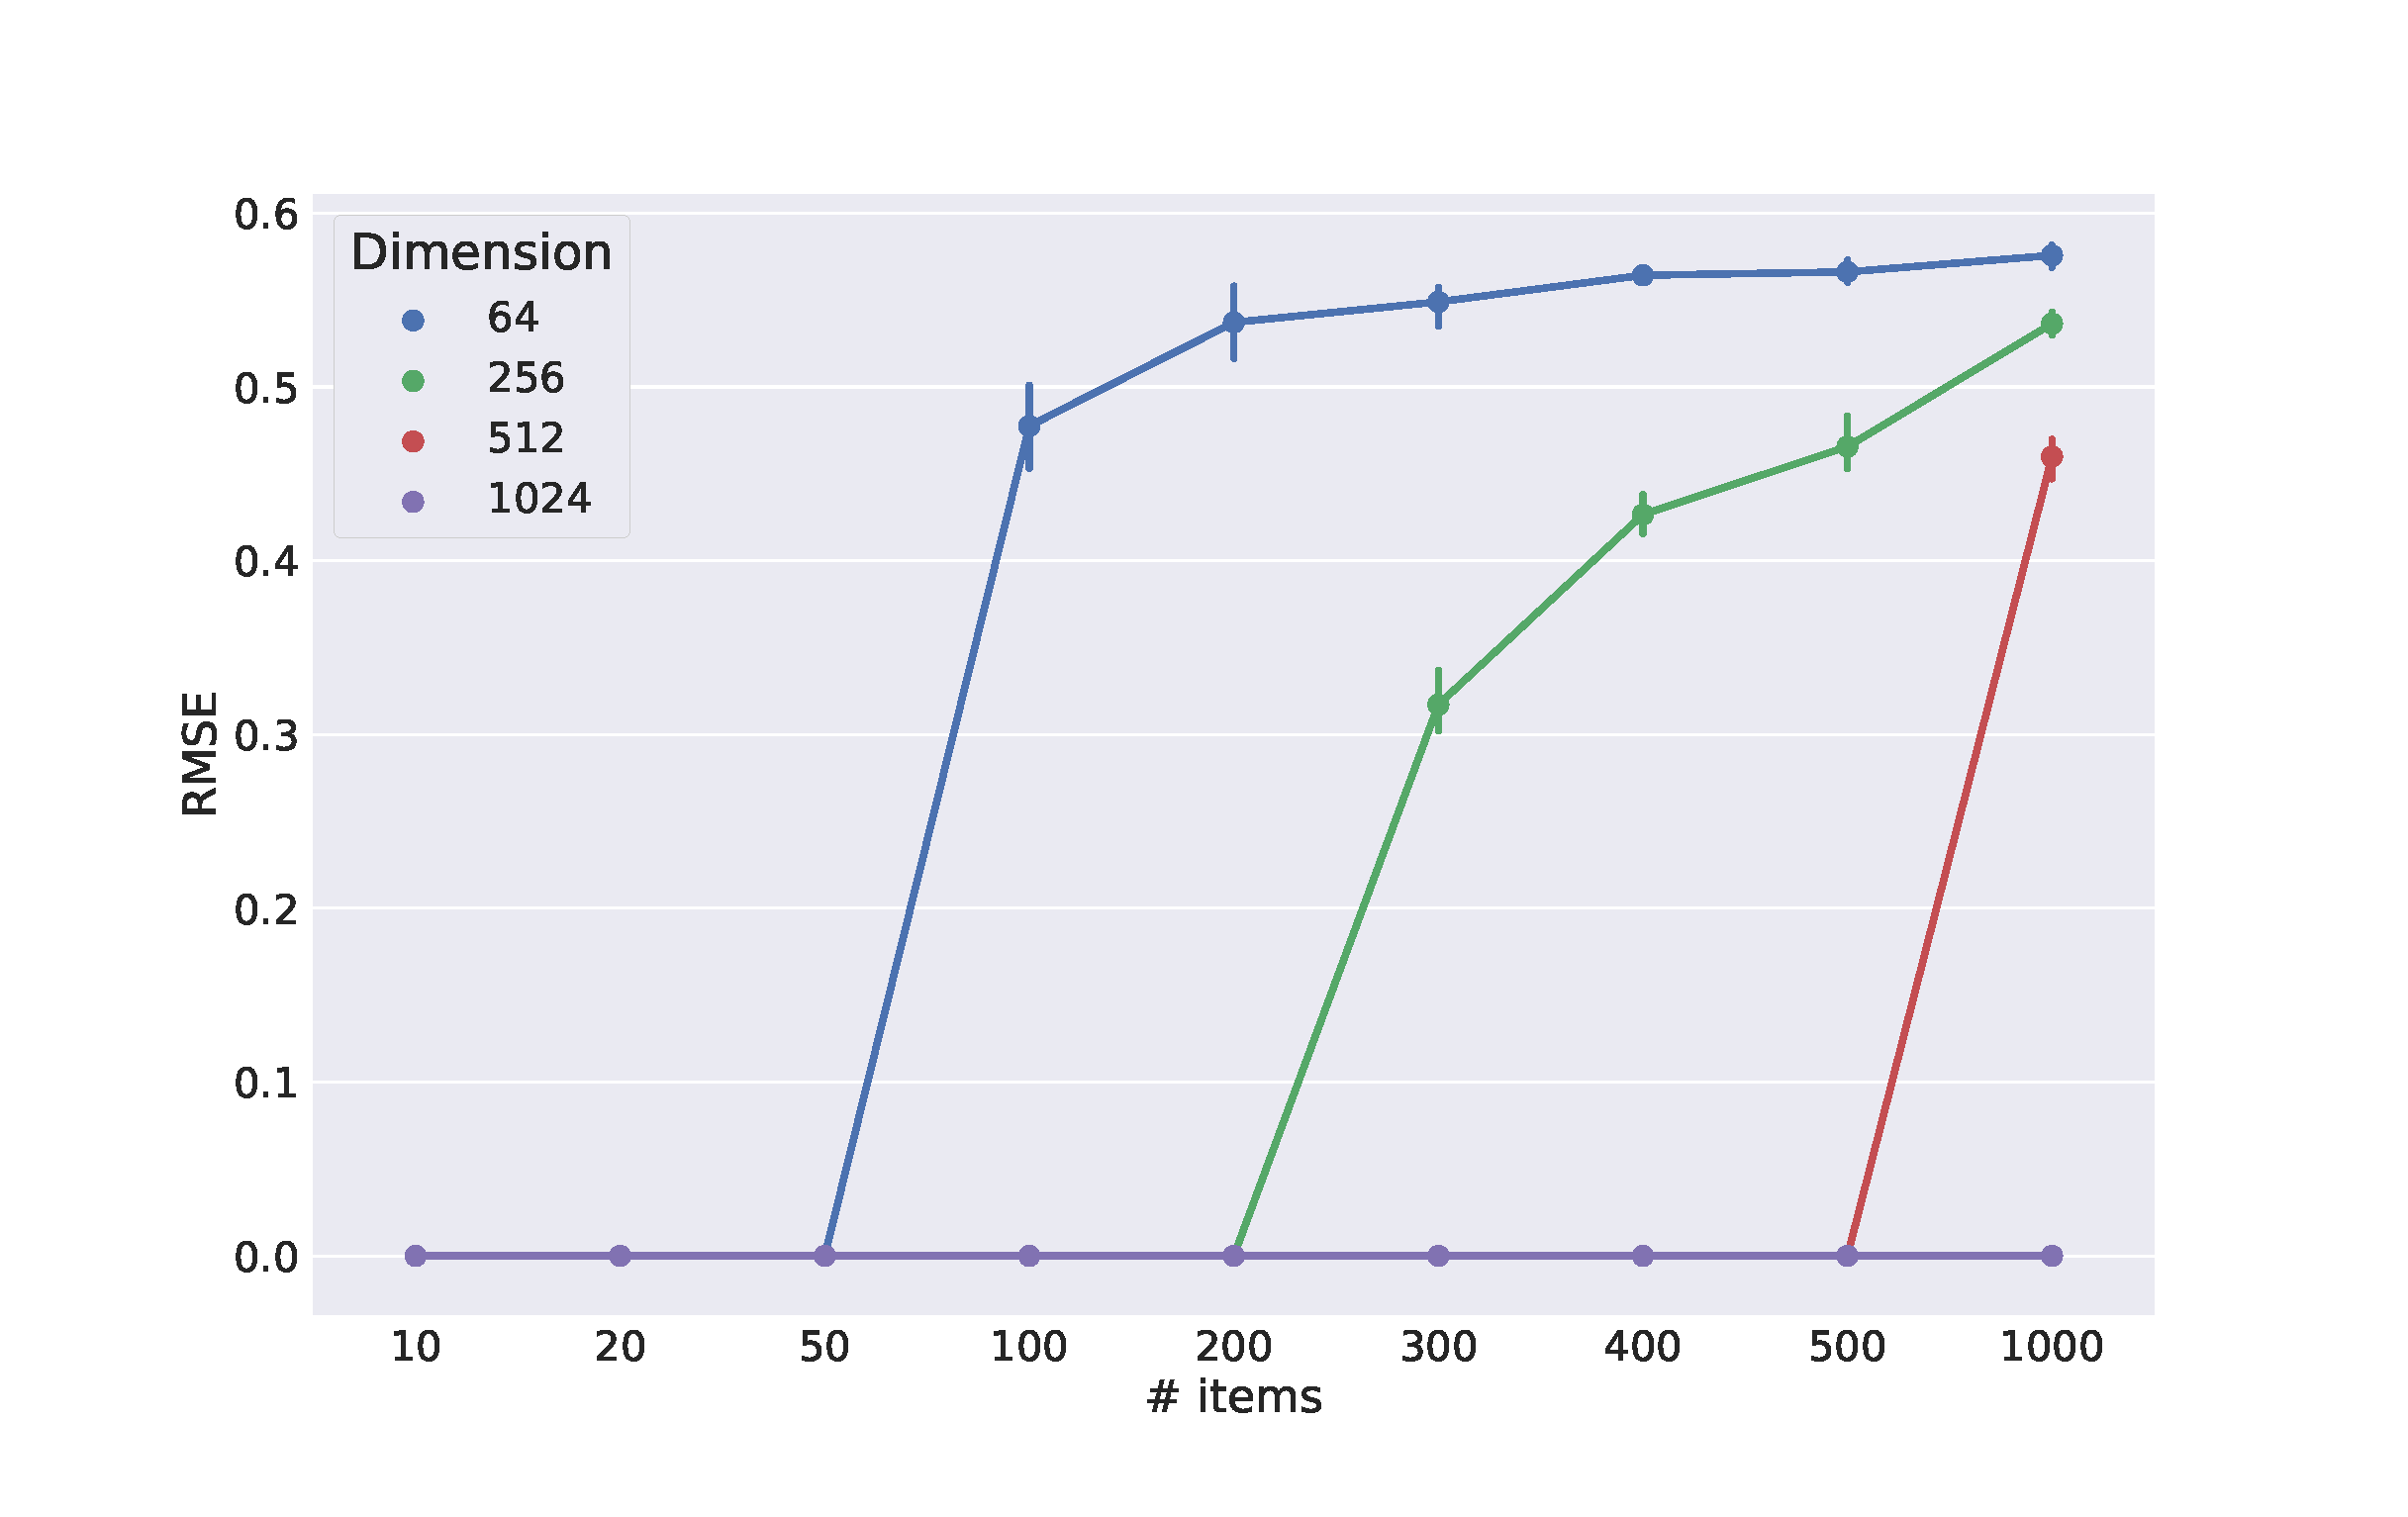
\includegraphics[width=0.5\linewidth]{imgs/scalar_encoding_decoding_rmse.eps}
    }
    \subfloat[\label{subfig:scalar_encoding_norm}]{%
        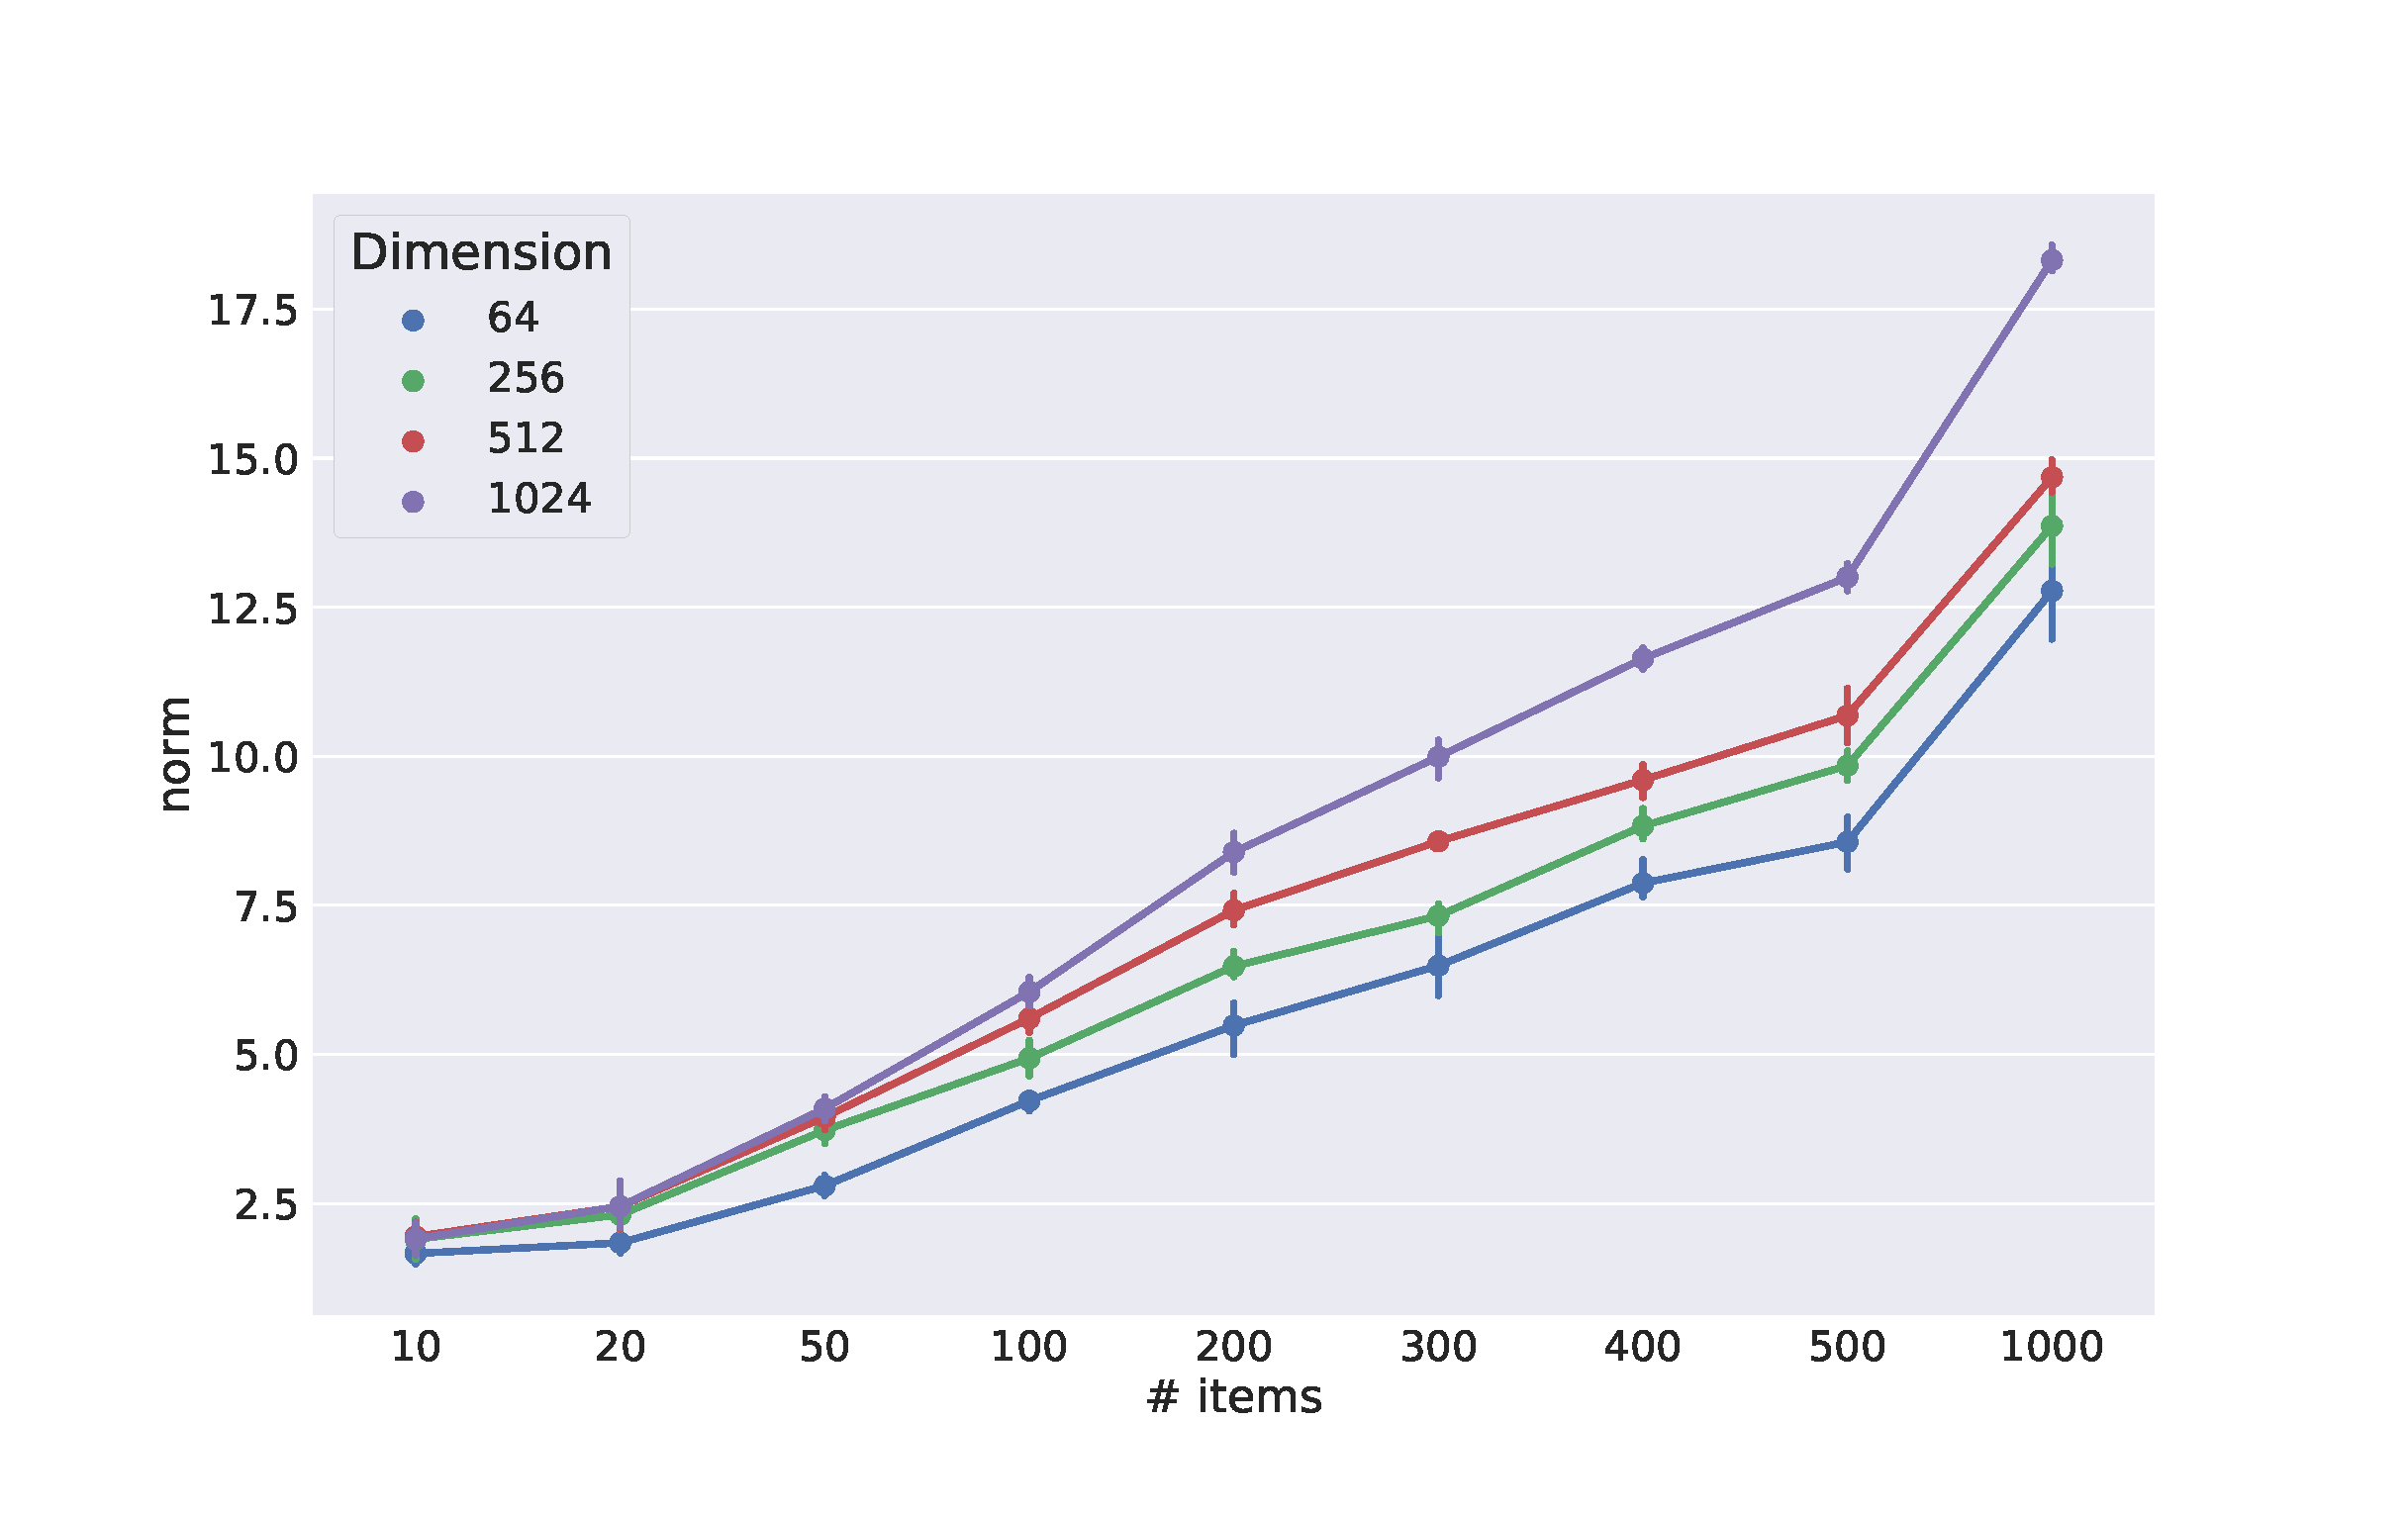
\includegraphics[width=0.5\linewidth]{imgs/scalar_encoding_norm.eps}
    }
    \caption{Properties of the simple scalar multiplication encoding of numerical values in vectors.~\protect\subref{subfig:scalar_encoding_decoding_rmse} shows the \ac{RMSE} when decoding back out an approximation of the original numerical values from the vector representation.~\protect\subref{subfig:scalar_encoding_norm} shows the norm of the representation vectors.}
    \label{fig:scalar_multiplication_encoding}
\end{figure}
Apart from encoding numerical values in vectors as the only non-zero elements within a vector containing only zero elements elsewhere, possibly the simplest encoding is to (for instance, randomly) choose vectors representing the desired entity/unit to be encoded and simply multiply all elements of that vector with the number the vector should represent.
Hence, to encode a sequence $a_{1}, \ldots, a_{n}$ of numerical values in vectors, we create a vocabulary of vectors $\mathcal{V}=\left\{ \mathbf{X}_{1}, \ldots, \mathbf{X}_{n} \right\}$ representing the corresponding units and multiply them by the scalar values with the vectors representing the units $a_{i}\cdot \mathbf{X}_{i}$.
Finally, summing up all of these vectors generates one single vector encoding all of the numerical values $a_{1}, \ldots, a_{n}$ 
\begin{equation}
\label{eq:scalar_mult_encoding}
\mathbf{V} = \sum\limits_{i=1}^{n} a_{i}\cdot \mathbf{X}_{i}. 
\end{equation}

For $\mathbf{X}_{i} = \left(x_{i0}, \ldots, x_{iD-1}\right)^{\intercal}$, this encoding is equivalent to the linear map given by the matrix $ \mathbf{M} $ consisting of the elements of the vectors $ \mathbf{X}_{i}$ column-wise concatenated

\begin{equation}
\label{eq:scalar_encoding_linear_map}
\mathbf{V} = \underbrace{\left(
\begin{matrix}
    x_{10} & \ldots & x_{n0} \\
    \vdots & \ddots & \vdots \\
    x_{1D-1} & \ldots & x_{nD-1} \\
\end{matrix}
\right)}_{=: \mathbf{M} } \cdot \left(
\begin{matrix}
a_{1} \\
\vdots \\
a_{n}\\ 
\end{matrix}
\right)
\end{equation}

Hence, we can use the inverse matrix $ \mathbf{M}^{-1}$ to decode back out an approximation $\hat{a}_{1}, \ldots, \hat{a}_{n}$ of the original numerical values $a_{1}, \ldots, a_{n}$ from the vector $ \mathbf{V}$ by $ \mathbf{V} \cdot \mathbf{M}^{-1}$.

The error of that approximation depends on the dimension $D$ of the underlying vector space and the number of numerical values encoded in the representation.
To analyze this error, we randomly choose numerical values $a_{1}, \ldots, a_{n}$ uniformly from the interval $ \left[0, 1\right)$ for $n=10, 20, 50,100,200,300,400,500,1000$ to be encoded as well as random, unit-length vectors $\mathbf{X}_{1}, \ldots, \mathbf{X}_{n}$ representing the numerical units, decode back out the approximations $\hat{a}_{1}, \ldots, \hat{a}_{n}$ of the original values and calculate the \ac{RMSE} between the actual values and their decoded approximations.
Figure~\ref{subfig:scalar_encoding_decoding_rmse} visualizes the results of this analysis for four different random trials for each vector dimension  $D=64, 256, 512, 1024$.
We observe that we can reliable decode back out up to $50, 200, 500$ and \num{1000} numerical values from the scalar multiplication encoding for vectors of dimension $64, 256, 512$ and \num{1024} respectively with an error in the order of magnitude of \num{e-14}, which is more than enough for our purposes.
However, Fig.~\ref{subfig:scalar_encoding_norm} shows one of the drawbacks of the scalar multiplication encoding scheme.
Although we choose the numerical values to be encoded to be lower than \num{1}, the norm of the resulting vectors becomes comparatively large for increasing vector dimension and number of numerical values encoded.
This makes sense, as we sum up an increasingly large number of vectors having the numerical values as their length.
This behavior will be reinforced if we use larger numerical values to be encoded.
Another potential drawback is that we need to calculate an entire inverse matrix to decode back out the original information from the vector representation, whereas one of the key strengths of \acp{VSA} is that of decoding back out information using the \ac{VSA}' binding operation and (pseudo-) inverse vectors (see Equation~\eqref{eq:retrieval}).

\subsubsection{Convolutive power encoding}%
\label{ssubsec:convolutive_power_encoding}

In this section, we present the final and, for this work most important, encoding scheme for numerical values, which we call the \emph{convolutive power encoding}.
The basic idea is to encode a numerical value $p \in \mathbb{R} $ as the power of a vocabulary vector $ \mathbf{X} $ representing the corresponding unit, i.e., $ \mathbf{X}^{p} $.
While defining the power of a vector $ \mathbf{X}^{n} $ is straightforward for an integer exponent $ n \in \mathbb{N} $,
\begin{equation}
\label{eq:vector_power_integer}
\mathbf{X}^{n} := \underbrace{ \mathbf{X} \varoast \mathbf{X} \varoast \ldots \varoast \mathbf{X} }_{\textrm{$n$ times}},
\end{equation}
it is not as intuitive for real-valued exponents $a \in \mathbb{R} $.
Therefore, we revisit the convolutive vector power given in definition~\ref{def:conv_power} 
\begin{equation}
\label{eq:conv_power}
v^{p} := \Re\left(\acs{IDFT} \left(\left(\acs{DFT}_{j}\left(v\right)^{p}\right)_{j=0}^{D-1}\right)\right),
\end{equation}
where $\Re$ denotes the real part $a$ of a complex number $a + ib \in \mathbb{C}$.
Equation~\eqref{eq:conv_power} enables us to encode numerical, real-numbered values $p \in \mathbb{R} $ as convolutive power $ \mathbf{X}^{p}$ and multiple numerical values $ p_{1}, \ldots, p{n}$ as
\begin{equation}
\label{eq:conv_power_several}
\mathbf{V} = \mathbf{X}_{1}^{p_{1}} \varoast \mathbf{X}_{2}^{p_{2}} \varoast \ldots \varoast \mathbf{X}_{n}^{p_{n}}.
\end{equation}
However, as we aim to avoid the issue of growing vector lengths when encoding a increasing number of numerical values mentioned for the scalar multiplication encoding, we restrict the vectors representing the units of the numerical values to be \emph{unitary} vectors.
Revisiting definition~\ref{def:unitary_vec} and lemma~\ref{lemma:unitary_vec}, a vector $ \mathbf{U}$ whose inverse element $ \mathbf{U}^{-1} $ is equal to its pseudo-inverse element $ \bar{\mathbf{U}} $ is called unitary.
Regarding the encoding of numerical values through their power, unitary vectors have some desirable properties (cf.\ lemma~\ref{lemma:unitary_vec}): 
\begin{itemize}
    \item unitary vector have unit length, i.e., $\norm{ \mathbf{U} }=1$,
    \item the power of a unitary vector is again unitary, i.e., the set of unitary vectors $ \mathcal{U} $ is closed under convolutive exponentiation,
    \item the product of two unitary vectors is again unitary,
    \item convolution with unitary vectors preserves the norm of the vector they are convolved with.
\end{itemize}

Given these properties, any vector created using Equation~\eqref{eq:conv_power_several} representing numerical values is a unitary vector with all its desirable properties.
Hence, we indeed avoid the problem of growing vector norm posed by the scalar multiplication encoding.

\begin{figure}[t]
    \centering
    \subfloat[\label{subfig:spa_power_representation_one_item}Convolutive power encoding for one two-dimensional numerical entity]{%
        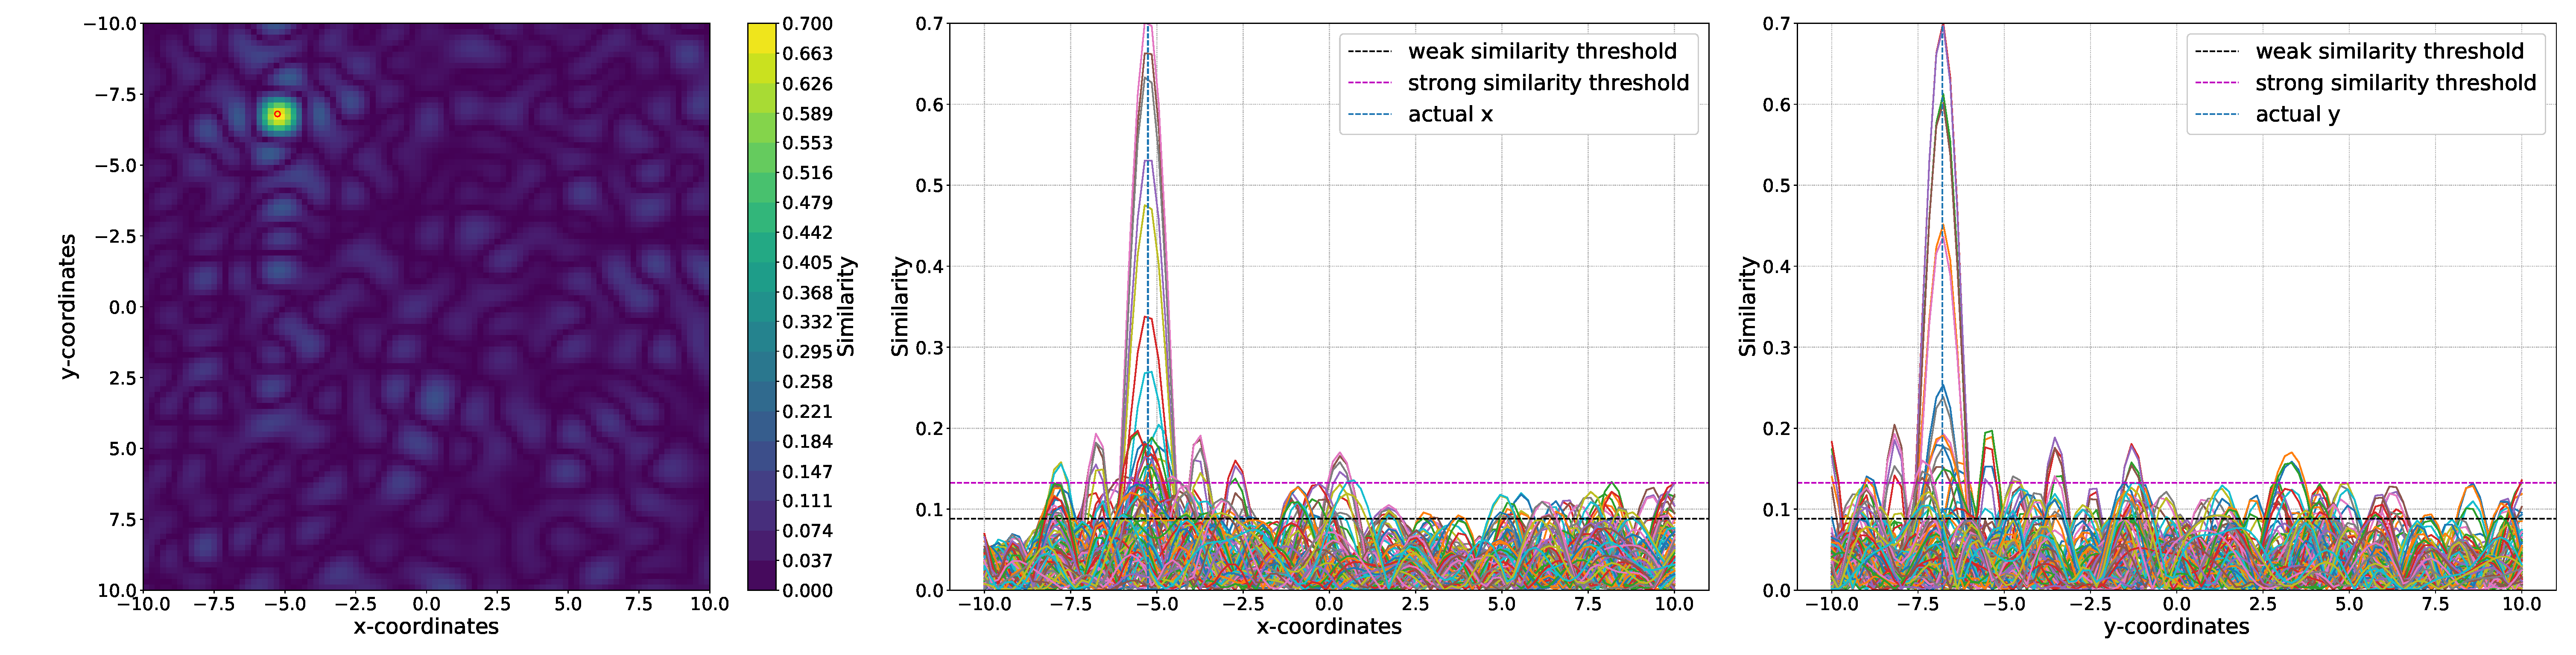
\includegraphics[width=0.9\linewidth]{imgs/spa_power_representation_one_item.eps}
    }\\
    \subfloat[\label{subfig:spa_power_representation_two_items}Convolutive power encoding for two two-dimensional numerical entities]{%
        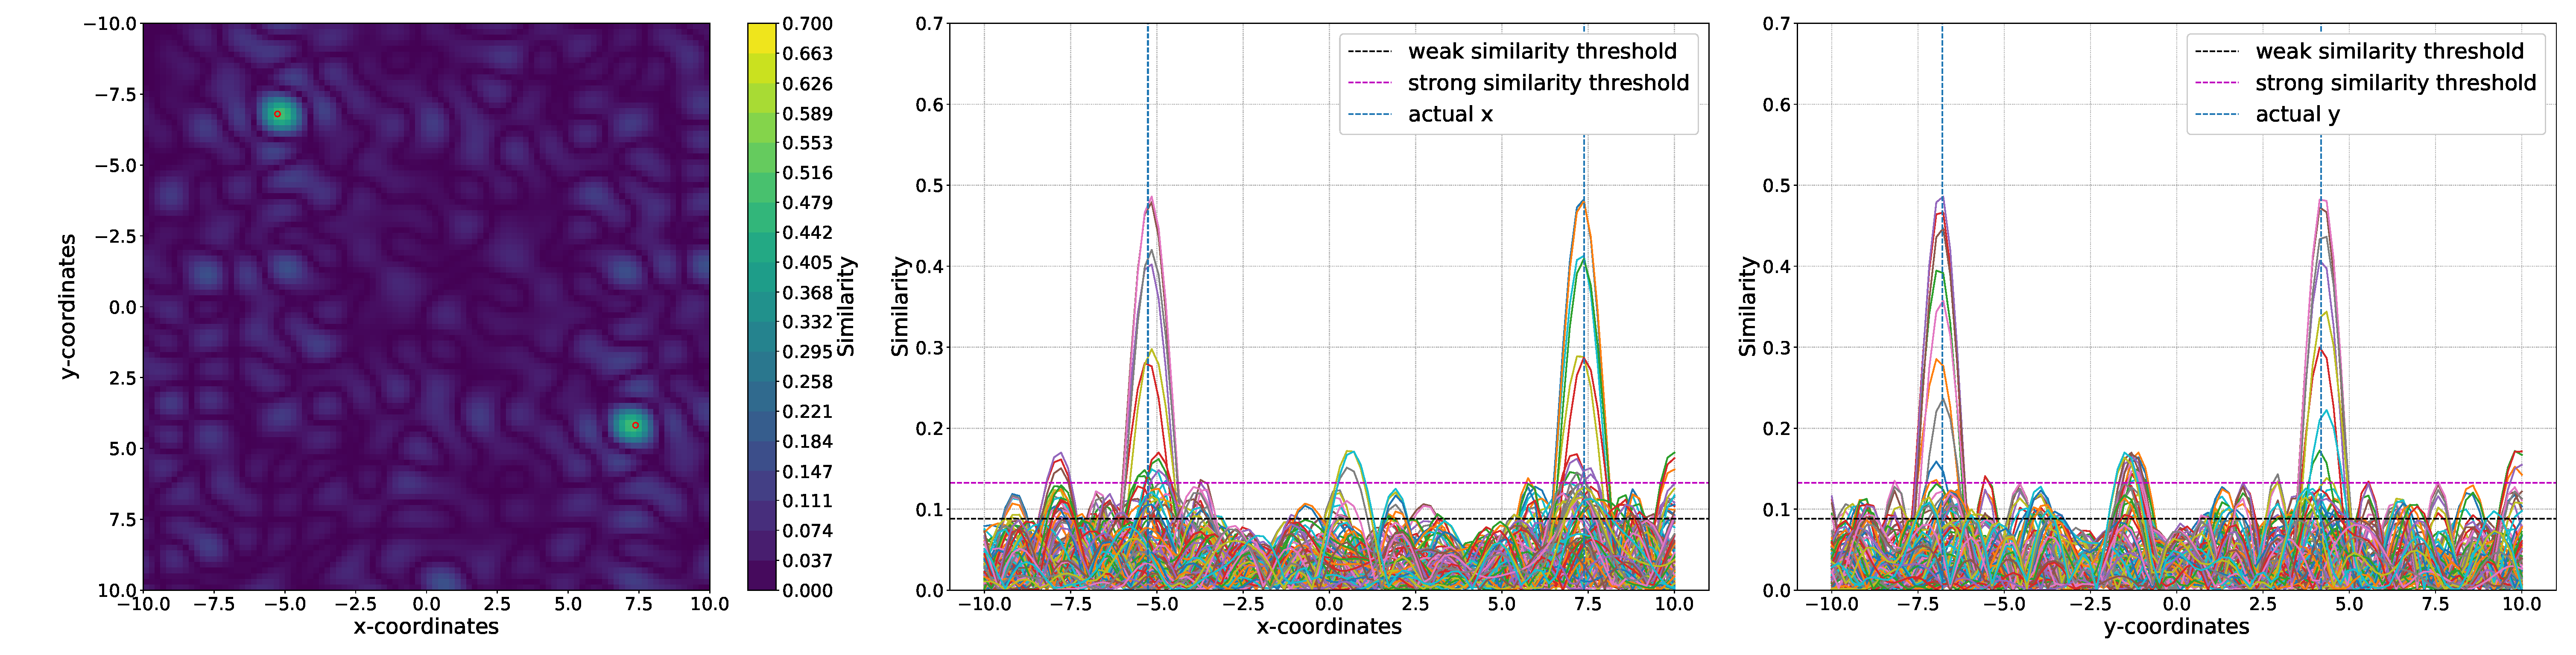
\includegraphics[width=0.9\linewidth]{imgs/spa_power_representation_two_items.eps}
    }
    \caption{
        Visualization of the convolutive power encoding scheme for \num{512}-dimensional representation vectors depicting the similarity between the representation vector and auxiliary comparison vectors created from a sequence of discrete values.
        The left plot in both rows shows a two-dimensional grid of the similarities, while the middle and right plot show the individual entities respectively.
        The red circles in the left plot and the dashed blue lines in the middle and right plots indicate the
    actual encoded values.}
    \label{fig:spa_power_encoding}
\end{figure}

As mentioned previously, we are primarily interested in a way of encoding two-dimensional values in vectors, which is why we focus our analysis of the convolutive power encoding scheme on this case.
Hence, we encode two numerical values $x,y$, i.e., a two-dimensional entity, by generating two random, unitary vectors $ \mathbf{X}, \mathbf{Y} $ representing the corresponding units and applying Equation~\eqref{eq:conv_power_several} 
\begin{equation}
\label{eq:conv_power_2d}
\mathbf{V} = \mathbf{X}^{x} \varoast \mathbf{Y}^{y}.
\end{equation}
To encode a sequence $ \left(x_{i}, y_{i}\right) $ for $i=1, \ldots, n$ of two-dimensional numerical values all sharing the same units, we simply sum up a their individual encoding vectors generated via Equation~\eqref{eq:conv_power_2d}, which leads to
\begin{equation}
\label{eq:conv_power_sum}
\mathbf{V} = \sum\limits_{i=1}^{n} \mathbf{X}^{x_i} \varoast \mathbf{Y}^{y_i}
\end{equation}
Figure~\ref{fig:spa_power_encoding} visualizes vectors encoding one (cf.\ Fig.~\ref{subfig:spa_power_representation_one_item} and Equation~\eqref{eq:conv_power_2d}) and two numerical entities (cf.\ Fig.~\ref{subfig:spa_power_representation_two_items} and Equation~\eqref{eq:conv_power_sum}) given by two units within one vector.
To generate the similarities shown in Fig.~\ref{fig:spa_power_encoding}, we calculate the dot product between the vectors actually representing the encoded values and vectors $ \tilde{\mathbf{V}}_{i} = \mathbf{X}^{\tilde{x}_{i}} \varoast \mathbf{Y}^{\tilde{y}_i} $ encoding a sequence of discrete sample values $ \left( \tilde{x}_{i}, \tilde{y}_{i} \right)$ for $i=1, \ldots, m$.
The left plot in each row of Fig.~\ref{fig:spa_power_encoding} depicts the similarities as heat map over a two-dimensional grid. 
The middle and right plots in Fig.~\ref{fig:spa_power_encoding} visualize the similarities of each unit, which is similar to plotting the heat map in three dimensions as ridges and slicing them through one of the ground axes.
In both rows, we observe high similarity peaks way above both similarity thresholds at the actual encoded values and significantly lower similarity values everywhere else.
However, we already encounter one of the problems of this encoding scheme.
Comparing the similarities at the positions of the encoded values, we observe a drop of similarity values from roughly \num{0.7} to \num{0.5} when encoding two two-dimensional numerical values instead of only one.
Thus, there is a limit of how many values can effectively be encoded in such a representation before noise becomes predominant and the encoded values can not be properly recovered anymore.
Such limitations regarding the number of concepts that can be represented in one vector depending on its dimension are a recurrent theme in the field of \acp{VSA}. 
Furthermore, we picked a $20 \times 20$ grid to encode numerical values using the convolutive power, which shows promising representational features here.
Although we are dealing with real-world sensor measurements in our applications, which are naturally limited by the sensors' range or other physical constraints and/or can be re-scaled to a suitable numerical range, we still need to analyze further, if and why the chosen size of the grid is reasonable.
We will further investigate these limiting factors of our representation in section~\ref{subsec:capacity_analysis_limitations_to_vector_representations}.

\subsection{Structured representations}%
\label{subsec:structured_representations}

Assuming we have generated a suitable vocabulary of atomic vectors encoding the entities and concepts of interest in an automotive context (cf.\ section~\ref{sec:preprocessing_stage_generating_a_vocabulary}) as well as several options of how to encode numerical values in vectors, we are now in the position to encapsulate the content and context of driving situations in semantic vectors.
In general, we employ the \ac{SPA}'s algebraic operations to bind connected items and concepts together through circular convolution and to sum up independent concepts appearing alongside one another.
More particularly, we combine all principles for structured representations presented so far in this thesis: simple superposition to generate unordered sets of items by summing the representational vectors, encoding of bound concepts through role-value pairs as shown in section~\ref{subsec:encoding_struct} and the several approaches to encode numerical values in structured vector representations as shown in section~\ref{subsec:different_vector_representations_for_numerical_values}.
However, the setup of such a vector representation is highly dependent on the actual task to be solved as well as the data available to be encoded.
Thus, we will present and investigate our structured representations in detail for two particular tasks in automotive context, namely driving context classification and vehicle trajectory prediction, in separate chapters~\ref{chap:driving_context_classification} and~\ref{chap:behav_pred}.
However, before we proceed to applying our vector representations to specific automotive tasks, we need to analyze their systematical limitations regarding the amount of information that can effectively be encoded in semantic vectors.

\subsection{Capacity analysis - limiting factors to vector representations}%
\label{subsec:capacity_analysis_limitations_to_vector_representations}

In section~\ref{subsec:different_vector_representations_for_numerical_values} and on several other occasions, we have already seen that there are general and systematical limits for the amount of information that can be encoded in and effectively decoded from vector representations in \acp{VSA}.
Such limits are a reoccurring theme and an essential feature of such architectures as they allow for the modeling of realistic cognitive phenomena.
Considering human subjects for instance, the capacity to process and store information or concepts in short-term memory as well as other cognitive tasks is subject to numerical restrictions \parencite{Miller1956}.
Hence, numerical limitations of cognitive architectures like the \ac{SPA} or \acp{VSA} in general are one way of modeling the numerical restrictions to cognition observed in human subjects.
In the context of automated driving however, we need to analyze these restrictions imposed by the cognitive architecture applied to provide upper borders regarding the amount of information that can be stored in our vector representation.
In this section, we analyze these limits with the goal of finding bounds for, e.g., the number of concepts that can effectively be stored in a single vector before the accumulation of noise makes it impossible to retrieve the original individual vectors.

\subsubsection{Superposition capacity}%
\label{ssubsec:superposition_capacity}

\begin{figure}[t]
	\centering
	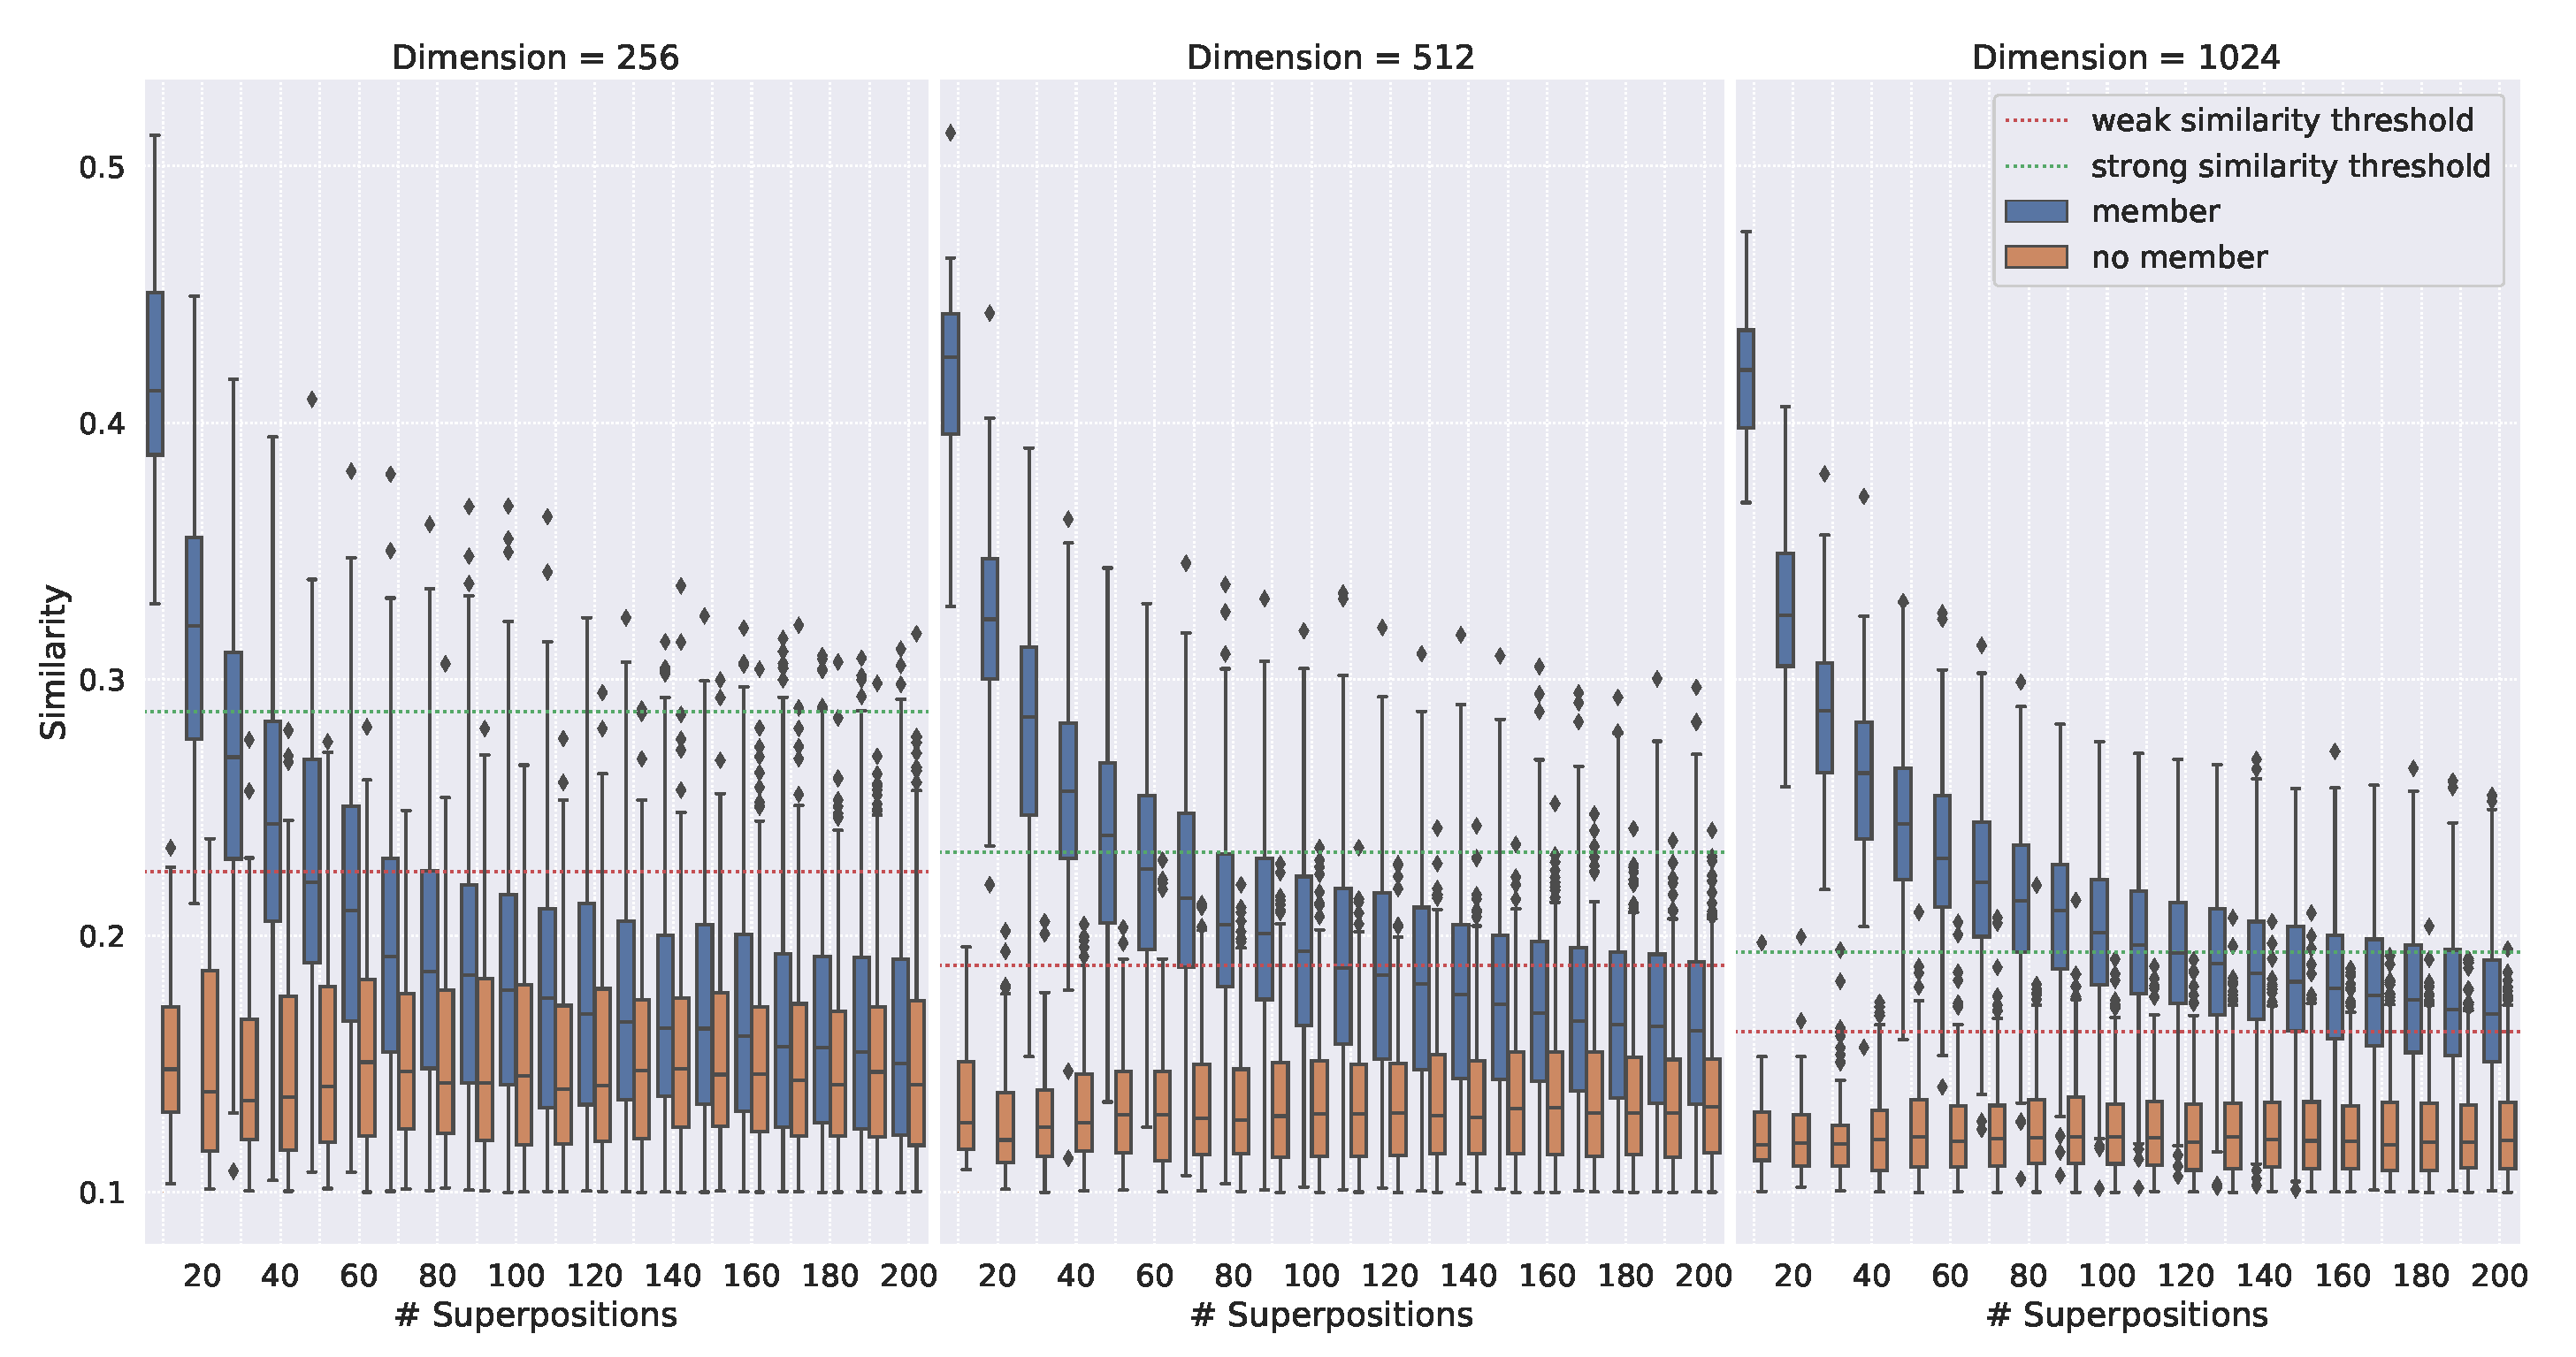
\includegraphics[width=0.95\textwidth]{imgs/spa_superposition_capacity.eps}
	\caption{Visualization of the \ac{SPA}'s superposition capacity for vector dimensions \num{256}, \num{512} and \num{1024}.
    The blue boxes indicate the similarity between the superposition vector and its summands, the orange boxes illustrate the similarity between the superposition vector and other randomly generated vectors.
    The dotted lines visualize the similarity threshold based on the vector dimensionality for reference.}
	\label{fig:spa_superposition_capacity}
\end{figure}

First, we evaluate the capacity of superposition, i.e., the addition operation of the \ac{SPA}.
Superposition is used to store and combine several concept vectors $ \mathbf{v}_i$ for $i=0, \ldots, n$ in an unordered set
\begin{equation}
\label{eq:superposition}
\mathbf{s} = \sum\limits_{i=0}^{n} \mathbf{v}_{i}.
\end{equation}
Given the properties of the \ac{SPA}, we can determine if a vector of interest $\mathbf{w}$ belongs to that ordered set by calculating the similarity $\phi\left( \mathbf{s}, \mathbf{w}\right)$ between the superposition vector and the vector of interest.
For sufficiently high-dimensional vectors, the similarity $\phi\left( \mathbf{s}, \mathbf{w}\right)$ will be close to \num{0} in case the vector $ \mathbf{w}$ is not part of the sum.
However, the more vectors we add to the superposition vector $ \mathbf{s}$, the more noise accumulates in the representation and thus decreases the similarity between the superposition vector $ \mathbf{s}$ and its individual ingredients $ \mathbf{v}_i$.
In order to analyze how many vectors can be added together by superposition before individual vectors become irretrievable, we conducted the following experiment: assuming we want to add $n$ vectors $ \mathbf{v}_i$ for $i=1, \ldots, n$ into a superposition vector $ \mathbf{s}$ as in Equation~\eqref{eq:superposition}, we randomly generate a vocabulary of $2n$ vectors $ \mathbf{v}_i$ for $i=1, \ldots, 2n$ and sum up the first $n$ members to create our superposition vector $ \mathbf{s}$.
Then we calculate the cosine similarity $\phi\left(\mathbf{s}, \mathbf{v}_i\right)$ between the superposition vector $ \mathbf{s}$ and every vector $ \mathbf{v}_{i}$ for $i=1,\ldots, 2n$ in the vocabulary.
A similar but slightly different experiment has been conducted by \textcite{Wahle2012}: the atomic vocabulary vectors,  referred to as elemental vectors in \textcite{Wahle2012}, are sparse in the sense, that they mostly contain \num{0} elements, and the superposed vectors are normalized after adding them.
Furthermore, \textcite{Wahle2012} only compare the similarity $\phi\left(\mathbf{s}, \mathbf{v}_1\right)$ between the superposition and the original vector with the similarity $\phi\left(\mathbf{v}_1, \mathbf{v}_n\right)$ between the original vector $ \mathbf{v}_1$ and the most recently added random vector $ \mathbf{v}_{n}$ as baseline for the expected similarity between randomly chosen vectors.
In contrast, although we have already analytically derived a threshold $\epsilon= \tfrac{c}{\sqrt{D}}$ for the expected similarity of randomly chosen vectors in definition~\ref{def:similar}, we calculate the similarity between the superposition vector and $n$ other random vectors for reference.

Figure~\ref{fig:spa_superposition_capacity} shows the result of our experiment for \num{3} random vocabularies per superposition length containing vectors of dimension \num{256}, \num{512} and \num{1024}.
The blue boxes in each figure illustrate the similarity between the superposition vector $ \mathbf{s}$ and each of the individual vectors $ \mathbf{v}_i$ for $i=1, \ldots, n$ it contains, i.e., the members of the unordered superposition set.
The orange boxes depict the similarity between $ \mathbf{s}$ and the other vocabulary vectors $ \mathbf{v}_i$ for $i=n+1, \ldots, 2n$ it does not contain, i.e., the non-members.
The dotted red and green lines indicate the \ac{SPA}'s weak and strong similarity threshold depending on the dimension of the vector space.
Considering the weak similarity threshold $\epsilon_{weak} = \tfrac{2}{\sqrt{D}}$, we observe that for a vector dimension of \num{256} the \ac{SPA} allows roughly \num{50} items to be stored in a superposition vector.
For higher vector dimensions \num{512} and \num{1024}, the number of items that can be superposed increases to roughly \num{100} and \num{200} respectively.
Considering the strong similarity threshold $\epsilon_{strong} = \tfrac{3}{\sqrt{D}}$, the upper borders for the number of items being stored in a superposition vector are slightly more conservative with \num{25}, \num{50} and \num{100} for vector space dimensions of \num{256}, \num{512} and \num{1024} respectively.
We also observe in our experiments that the similarity between the superposition vector and non-member random vectors is consistently below the weak similarity threshold $\epsilon_{weak}$ for the majority of the samples.
However, once the similarity between the superposition vector and its members drops below either of the similarity thresholds for the majority of the samples, we can not distinguish between members and non-members with a sufficiently high probability.
For \num{256} dimensional vectors for instance, we even observe that the members and non-members become nearly indistinguishably when adding more than \num{80} vectors.
Thus, we have to choose rather conservative bounds for the number of items to be encoded in a superposition vector.

\subsubsection{Capacity of structured representations involving convolutive powers}%
\label{ssubsec:capacity_of_structured_representations_involving_convolutive_powers}

\begin{figure}[t]
    \centering
    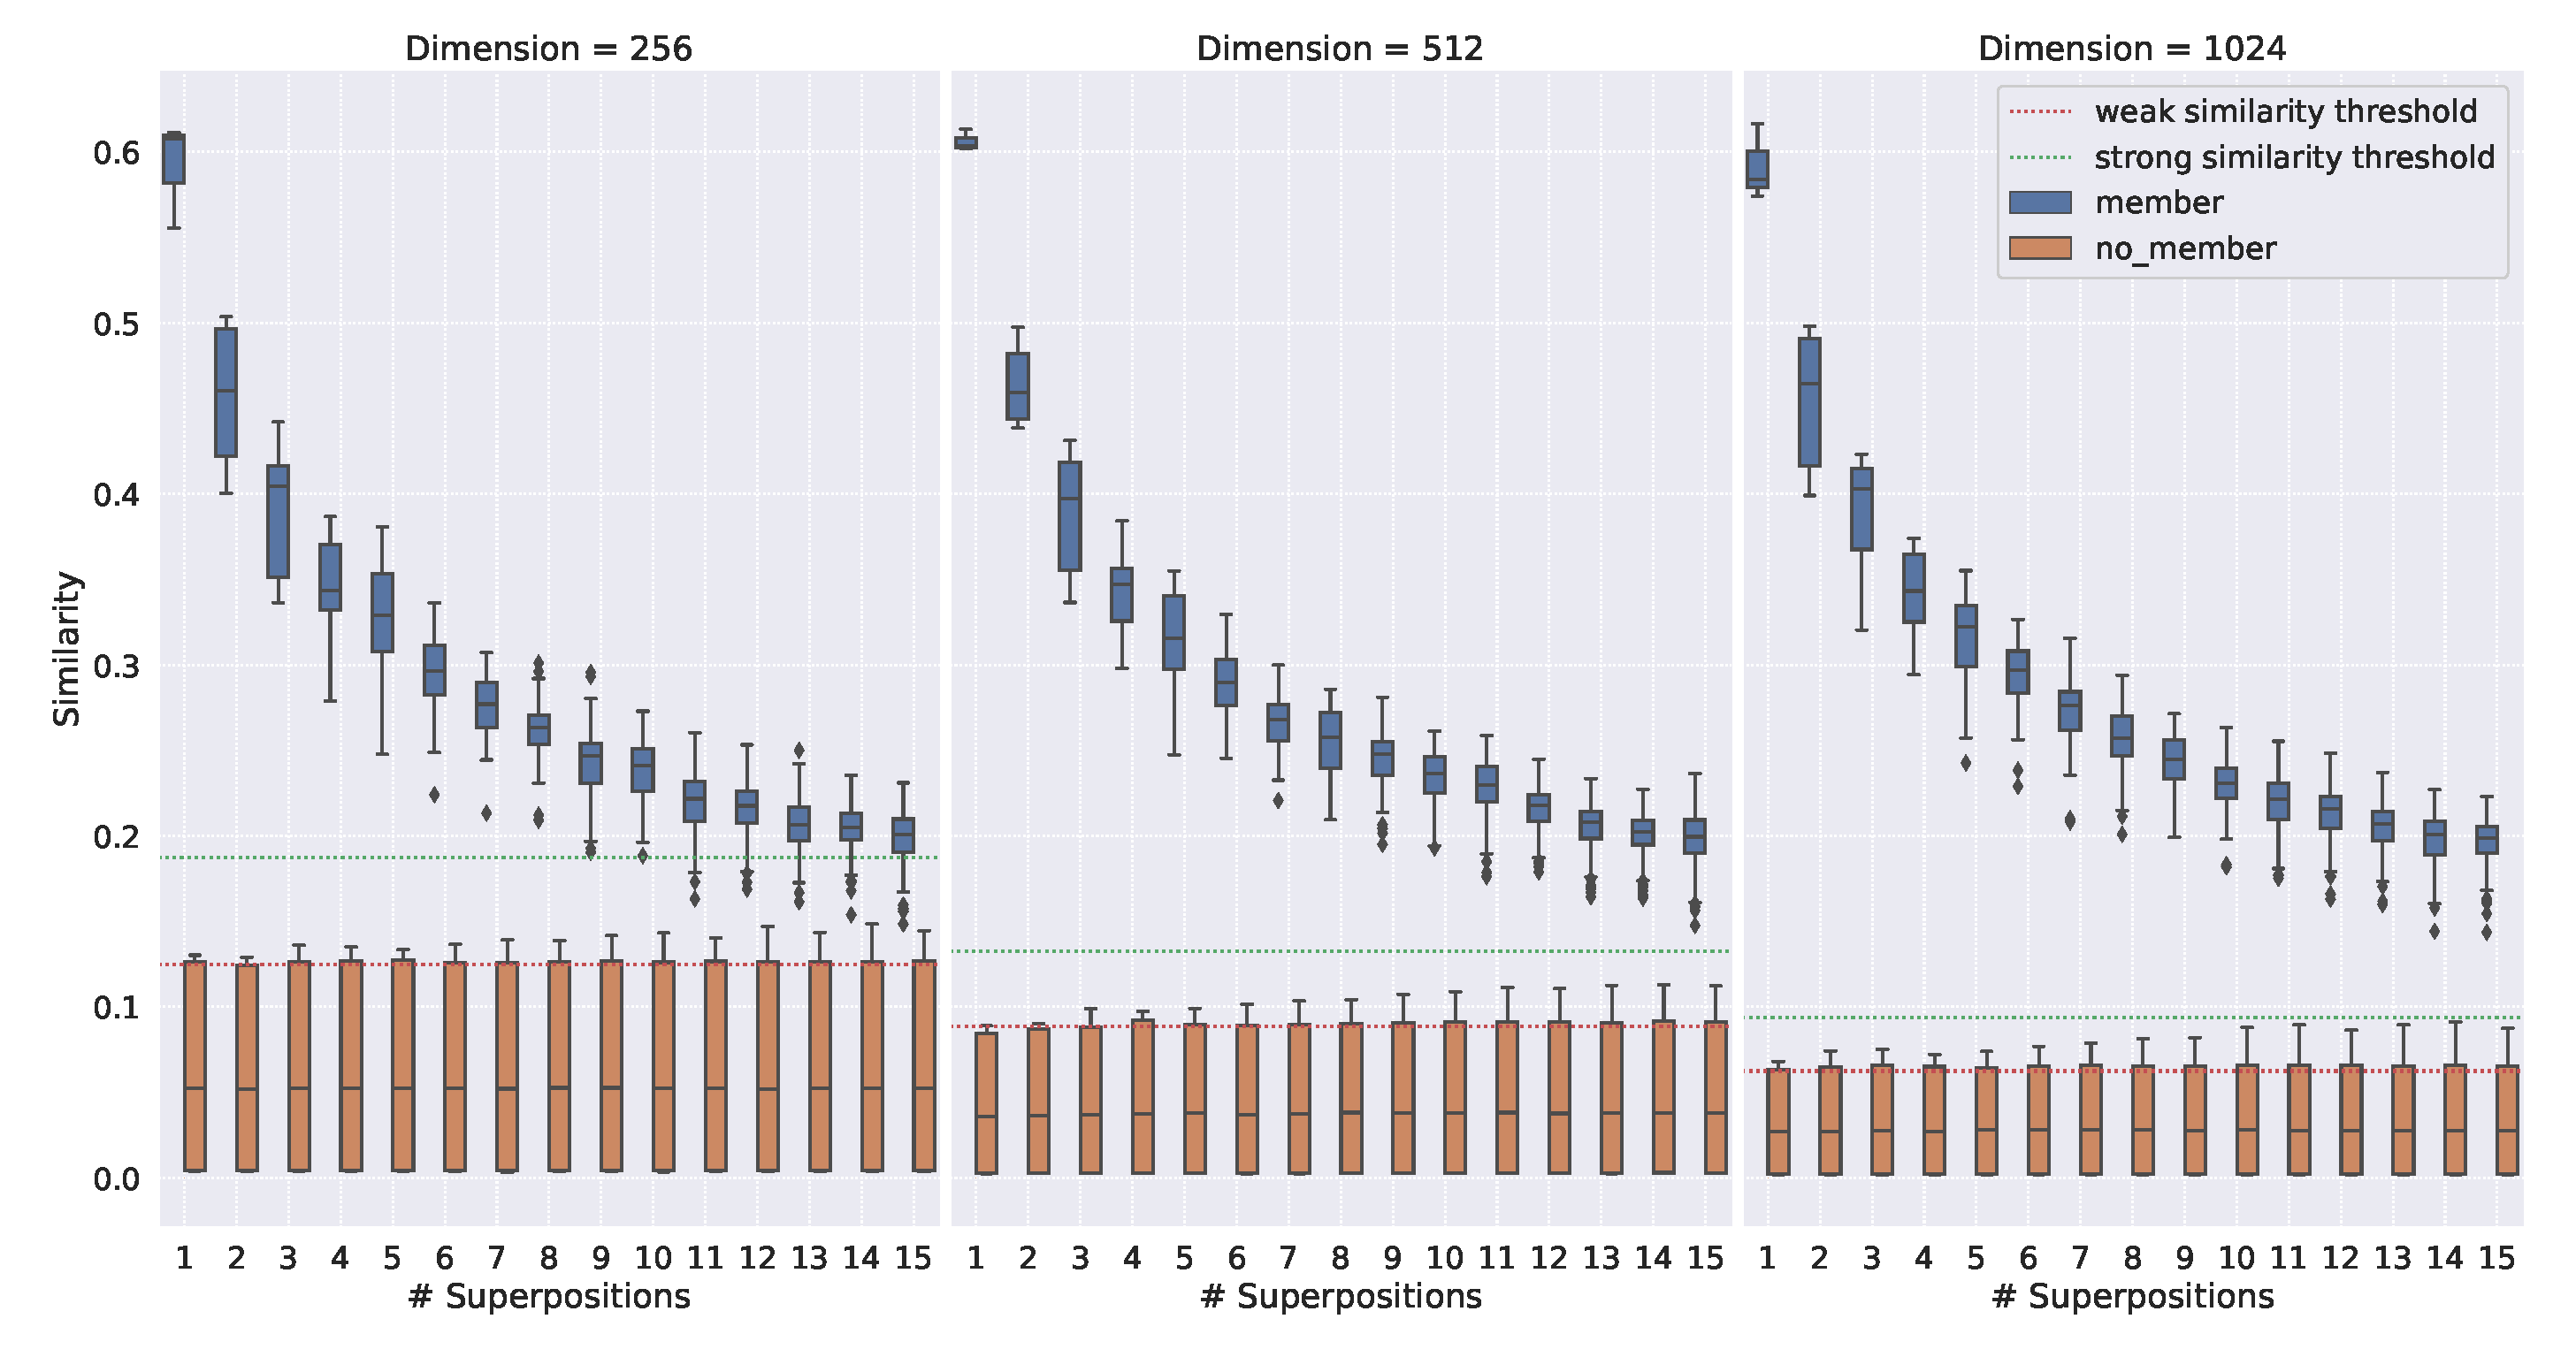
\includegraphics[width=0.95\linewidth]{imgs/spa_power_capacity.eps}
    \caption{Capacity analysis for the superposition of vectors encoding spatial positions using the convolutive vector-power for varying vector dimensions.}
    \label{fig:spa_power_capacity}
\end{figure}

In the previous section, we have analyzed the \ac{SPA}'s capacity regarding the number of items that can be stored in an unordered set using superposition.
For encoding driving situations in a semantic vector substrate, we will most likely employ more complex representation than superposition of single items alone.
In this section, we thus analyze the \ac{SPA}'s capacity regarding the structured representations involving the convolutive vector-power representation presented in section~\ref{subsec:different_vector_representations_for_numerical_values}.
Figure~\ref{fig:spa_power_encoding} has already shown, that unbinding positions back out by querying the representation vector with sample vectors encoding discrete position examples yields high similarities for samples in the region of the encoded values and low similarities elsewhere.
These low similarities for the particular examples shown in Fig.~\ref{subfig:spa_power_representation_one_item} and~\ref{subfig:spa_power_representation_two_items} are below or at most in the order of magnitude of the \ac{SPA}'s similarity thresholds.
However, we also observe, that encoding several entities of the same type in one position vector as in Fig.~\ref{subfig:spa_power_representation_two_items}, the similarities of the true positive positions decrease compared to the encoding of only one item as in Fig.~\ref{subfig:spa_power_representation_one_item}.
Hence, our capacity analysis not only has to cover the amount of objects encoded in one vector, but also the number of items per object class.

\begin{figure}[t]
    \centering
    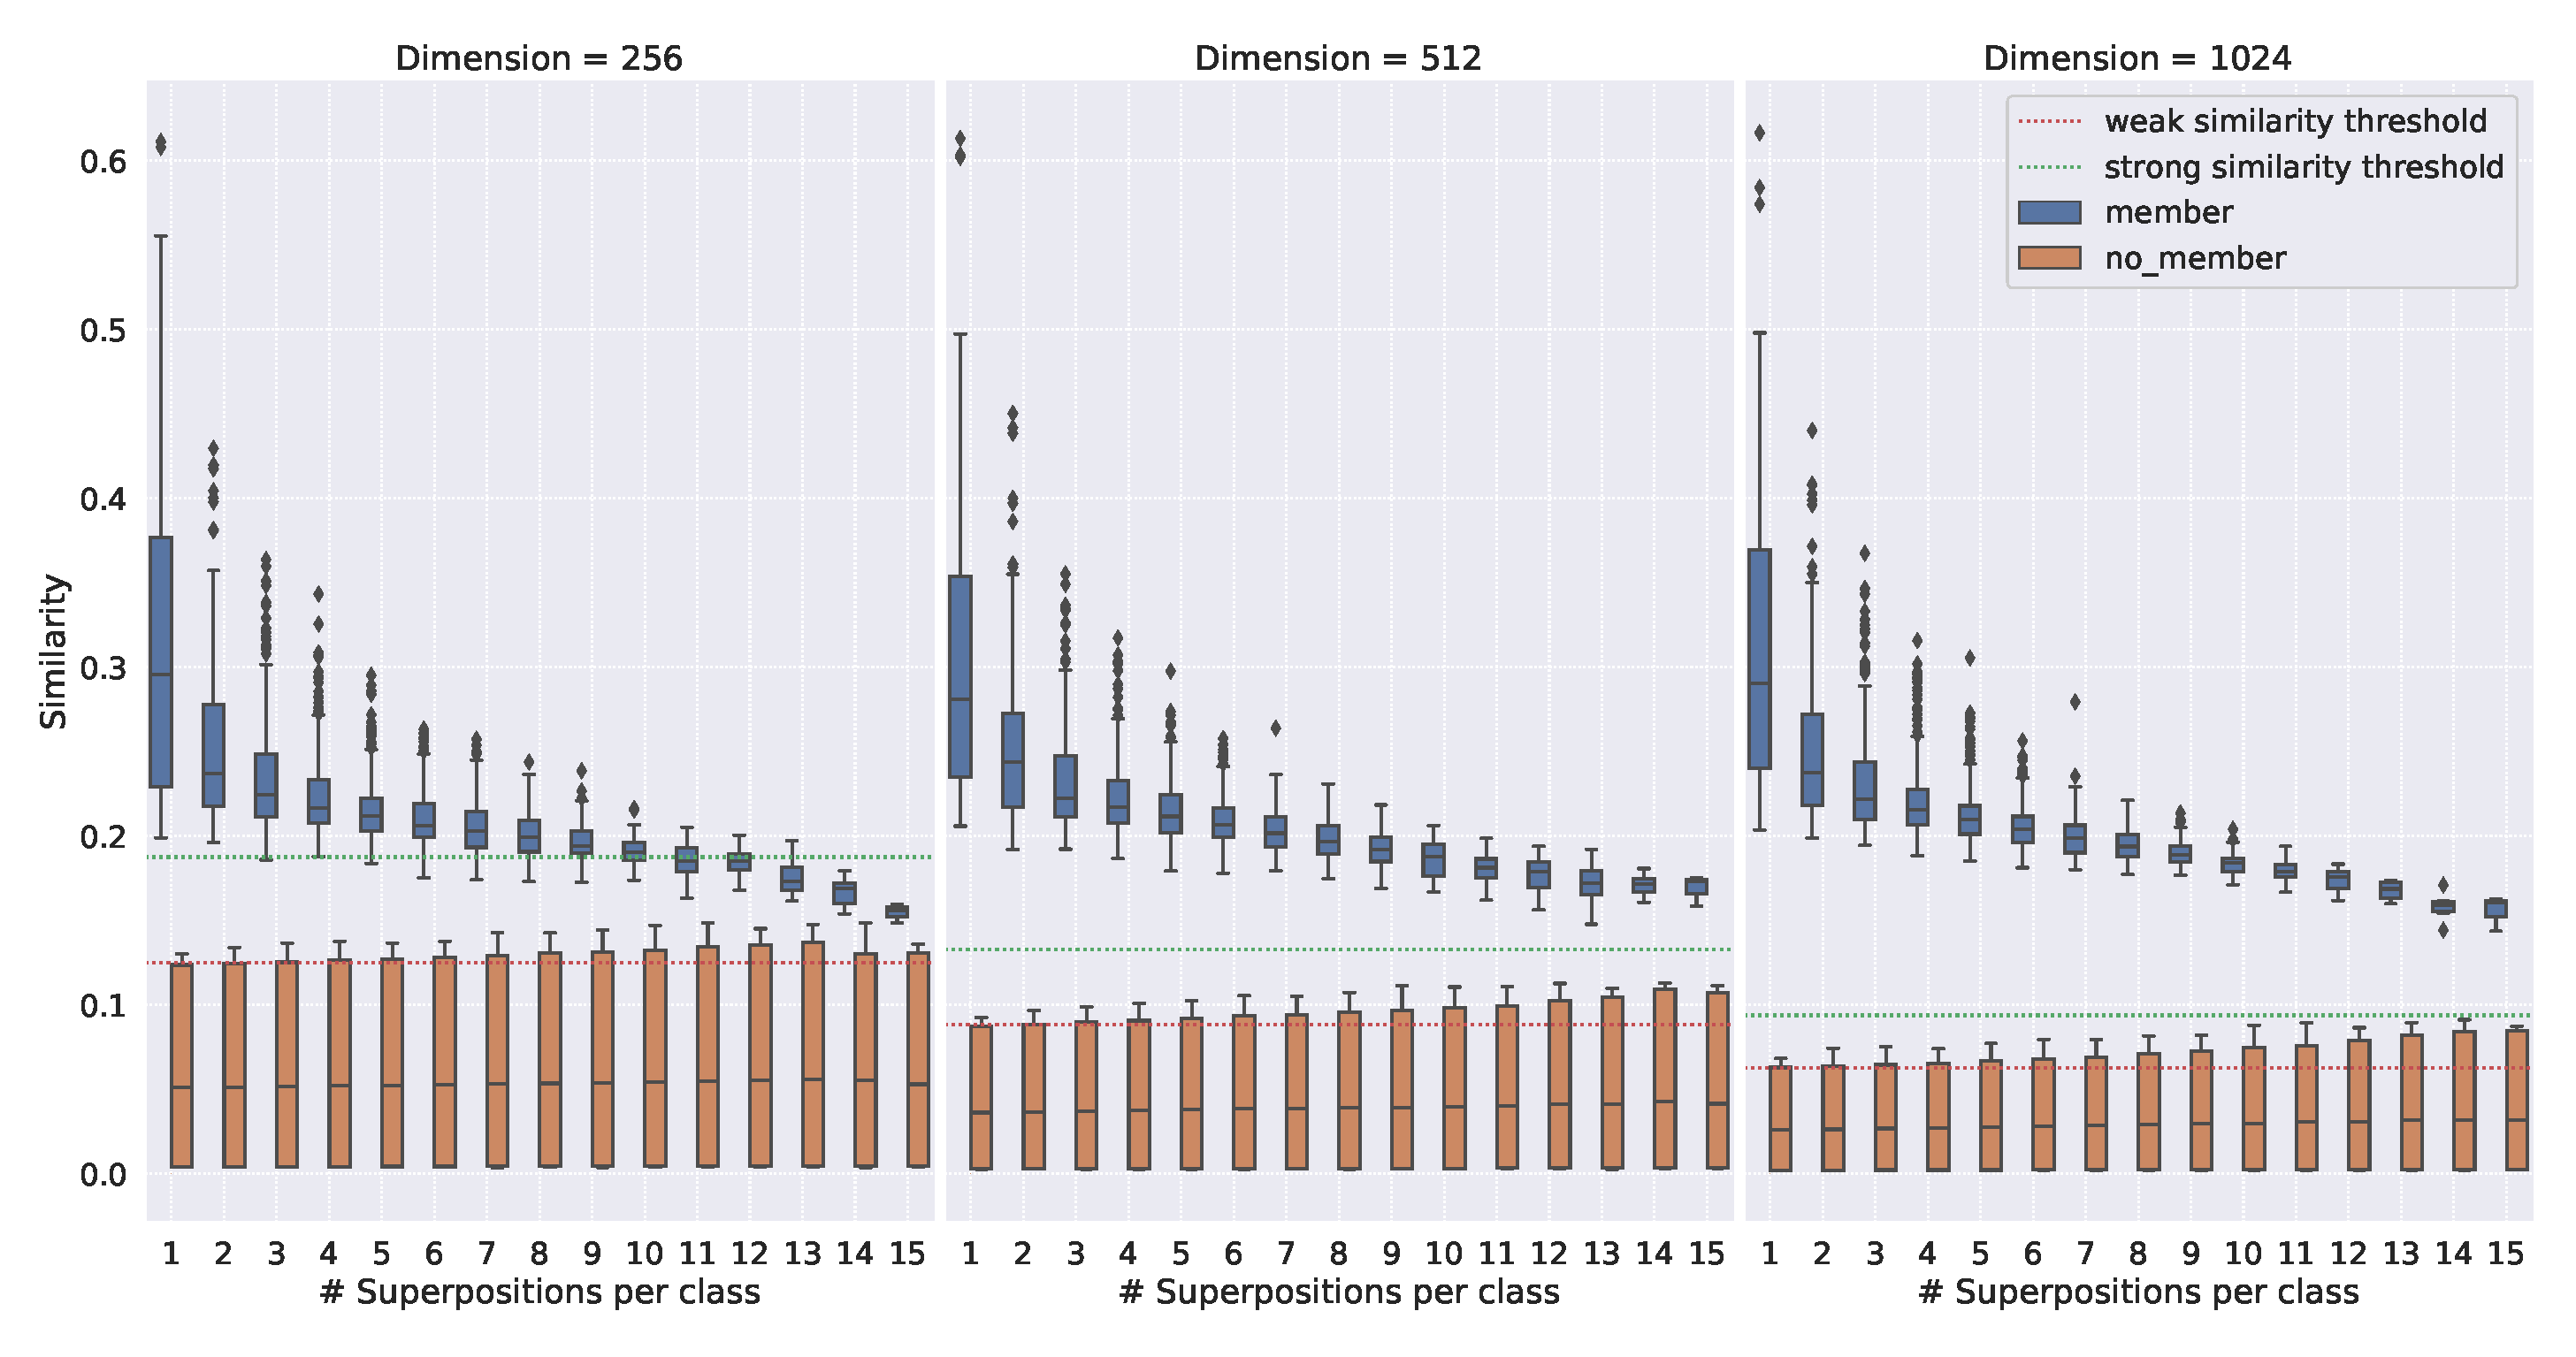
\includegraphics[width=0.95\linewidth]{imgs/spa_power_capacity_superpositions_per_class.eps}
    \caption{Capacity analysis for the superposition of vectors encoding spatial positions using the convolutive vector-power for varying vector dimensions.
        In contrast to Fig.~\ref{fig:spa_power_capacity}, this figure illustrates the similarity for vectors containing spatial information for several objects of the same class.
    }
    \label{fig:spa_power_capacity_superpositions_per_class}
\end{figure}

Therefore, we conduct the following experiment: assuming we want to encode $n$ spatial entities, i.e., objects $o_{i}$ with two-dimensional location information $ \left(x_{i}, y_{i}\right)$ for $i=1, \ldots, n$ as shown in Fig.~\ref{fig:spa_power_encoding} for $n=1$ (Fig.~\ref{subfig:spa_power_representation_one_item}) and $n=2$ (Fig.~\ref{subfig:spa_power_representation_two_items}), into a single representation vector $ \mathbf{s}$, we generate a vocabulary of random vectors $
\mathbf{v}_{i}$ for $i=1, \ldots, n$ encoding object class labels and random unitary vectors $ \mathbf{X}, \mathbf{Y}$ to encode the units of the spatial information.
In contrast to the previous experiment, where we simply summed up a certain number of random vectors, we are interested in a more specific analysis, since there are several possibilities to distribute the positional values $ \left(x_{i}, y_{i}\right)$ over the available object class vectors $ \mathbf{v}_{i}$.
For instance, for a total number of two superpositions, i.e., $n=2$, there are two possibilities to generate our representation vector, namely
\begin{align}
    \mathbf{s}_{1} &= \mathbf{v}_{1} \varoast \mathbf{X}^{x_{1}} \varoast \mathbf{Y}^{y_{1}} + \mathbf{v}_{1} \varoast \mathbf{X}^{x_{2}} \varoast \mathbf{Y}^{y_{2}}, \label{eq:spa_power_exp_v1} \\
    \mathbf{s}_{2} &= \mathbf{v}_{1} \varoast \mathbf{X}^{x_{1}} \varoast \mathbf{Y}^{y_{1}} + \mathbf{v}_{2} \varoast \mathbf{X}^{x_{2}} \varoast \mathbf{Y}^{y_{2}}. \label{eq:spa_power_exp_v2} 
\end{align}
The vector $ \mathbf{s}_{1}$ in Equation~\eqref{eq:spa_power_exp_v1} encodes two objects of the same type, while the vector $ \mathbf{s}_{2}$ encodes occurrences of two different object types at the given locations.
As we are working with random vectors in this experiment, we can, without loss of generality, skip the vector encoding two objects of type represented by the vector $ \mathbf{v}_{2}$, which would yield a result equivalent to Equation~\eqref{eq:spa_power_exp_v1}.
More generally, we are interested in all sets
\begin{equation}
\label{eq:sum_combinations}
C_{m,j} = \left\{0 < k_{1}, \ldots, k_{m} \leq n \quad | \quad m \leq n \textrm{ and } \sum\limits_{i=1}^{m} k_{i} = n \right\}
\end{equation}
of natural numbers $k_{i}$ summing up to $n$ ignoring permutations of the $k_{i}$. 
We index the sets with $j$, since there potentially exist several possibilities to decompose $n$ into sums of $m$ natural numbers.

In our experiments, for each number $n$ of total objects to be encoded in the vector representation, we calculate all possible sets $C_{m,j}$ (ignoring permutations) and generate random position values $ \left(x_{i}, y_{i}\right)$ for $i=1, \ldots, n$ and a random vocabulary as described above.
For each set $C_{m,j}$, we generate a representation vector 
\begin{equation}
\label{eq:spa_power_exp_v_gen}
\mathbf{s}_{m,j} = \sum\limits_{i=1}^{m} \sum\limits_{l=1}^{k_{i}} \mathbf{v}_{i} \varoast \mathbf{X}^{x_{i}} \varoast \mathbf{Y}^{y_{i}}
\end{equation}
as well as query vectors $ {\mathbf{P}}_{i} = \mathbf{X}^{\tilde{x}_{i}} \varoast \mathbf{Y}^{\tilde{y}_i} $ encoding a sequence of discrete sample values $ \left( \tilde{x}_{i}, \tilde{y}_{i} \right)$ for $i=1, \ldots, M$ evenly distributed over the length of the positional encoding grid.
In other words, Equation~\eqref{eq:spa_power_exp_v_gen} states, that each class label $ \mathbf{v}_{i}$ appears $k_{i}$ times yielding a sum of $n$ objects.
We query the representation vector for the position of each class by binding it to the pseudo-inverse element $ \bar{ \mathbf{v}}_{i}$ for each class label vector, i.e., 
\begin{equation}
\label{eq:spa_power_query}
\mathbf{s}_{m,j} \varoast \bar{ \mathbf{v}}_{i} \approx \sum\limits_{l=1}^{k_{i}} \mathbf{X}^{{x}_{i}} \varoast \mathbf{Y}^{{y}_i}, 
\end{equation}
and calculate the similarity with the discretized position vectors $ \mathbf{P}_{k}$ to get
\begin{equation}
\label{eq:text}
s_{i,k} = \left|\phi \left( \mathbf{s}_{m,j} \varoast \bar{ \mathbf{v}}_{i}, \mathbf{P}_{k}\right) \right|.
\end{equation}
For samples close to the originally encoded positions, i.e., $\left| x_{i} - \tilde{x}_{i}\right| < \epsilon$ and $\left| y_{i} - \tilde{y}_{i}\right| < \epsilon$ for a certain threshold $\epsilon$, we label $s_{i,k}$ as positive similarity denoting a member of the representation vector.
Otherwise, we consider the similarity $s_{i,k}$ at position $\left( \tilde{x}_{i}, \tilde{y}_{i} \right)$ not a member of the representation vector $ \mathbf{s}_{m,j}$.

Figure~\ref{fig:spa_power_capacity} shows the results of this capacity analysis regarding the total number of superposed objects within the representation vector for varying vector dimensions.
The blue boxes in each column illustrate the positive similarity values, i.e., for positions considered members of the representation vector, whereas the orange boxes indicate the negative similarity values of the non-member positions.
The dotted red and green lines visualize the weak and strong similarity threshold for each dimension respectively.
Similar to Fig.~\ref{fig:spa_power_encoding}, we observe that the similarity of the non-members is in the order of magnitude of the similarity thresholds while the similarity for the member position decreases with a growing number of spatial items encoded in the vector.

Figure~\ref{fig:spa_power_capacity_superpositions_per_class} shows a different evaluation of the same data showing the number of addition operations per class on the $x$-axis.
In contrast to Fig.~\ref{fig:spa_power_capacity}, Fig.~\ref{fig:spa_power_capacity_superpositions_per_class} illustrates the similarity for vectors containing spatial information for several objects of the same class.
That is, Fig.~\ref{fig:spa_power_capacity_superpositions_per_class} illustrates the similarity of vectors containing a specific number $n$ of superpositions per class on its $x$-axis independent of the total number of superpositions.
We observe, that not only the similarity of the members decreases with growing number of superpositions per class, but the similarity of the non-member increases beyond the weak similarity threshold.
Similar to the simple superposition capacity analysis, we consider the point in the plots where the member similarities fall below the strong similarity threshold the upper border for the maximal number of spatial objects per class to be encoded in this representational substrate.
For instance, this upper bound for \num{256} dimensional vectors is \num{10} superpositions per class, which is roughly half of the upper bound for the number of simple superpositions.

\section{Summary}%
\label{sec:vector_representations_automotive_summary}

In this chapter, we presented the general approach of creating structured vector representations to encode automotive scenes.
After showing the theoretical tool set in chapter~\ref{chap:introduction_to_vsas} independent of particular applications, we focused our attention to scene representation in automotive context.
The chapter's structure followed the process established by \textcite{Gallant2013} and is split into two main subsections focusing on the creation of vocabularies of atomic vectors (section~\ref{sec:preprocessing_stage_generating_a_vocabulary}) and generating structured, more complex representations from the atomic vectors in the vocabulary (section~\ref{sec:representation_generation_stage}).
We showed several approaches to generate vector vocabularies of entities encountered in automotive scenes such as traffic participants and traffic signs based on either manual design or automated learning.
Thereby, we were able to encapsulate different similarity structures such as visual similarity, semantic similarity and a fusion of both.
We were able to demonstrate, that we can successfully encapsulate the desired similarity structure within our vocabulary of atomic vectors.
Finally, we pointed out advantages and problems for both approaches to generate these structured vocabularies with the bias imposed by human engineers and limits regarding sufficiently large and available data sets being the main issues for manual and learned vocabularies respectively.
Since we consider the choice of a suitable vocabulary to be highly dependent on the particular task to be solved, we analyze the influence of varying the underlying vocabulary for the specific task of classifying the current driving context based on a vector representation of the current scene in section~\ref{subsec:the_influence_of_varying_vocabularies}.

In section~\ref{sec:representation_generation_stage}, we proceeded to investigate the creation of more complex, structured representations from atomic vocabulary vectors.
One of the most important aspects was the representation of numerical values in high-dimensional vectors, where we presented three different approaches and showed their individual strengths and limitations.
Particularly, we presented a novel approach to encode numerical values based the convolutive power of vectors.
The biggest advantage of this representation of numerical values is that it can be bound further to other vectors as well as be used to query representation vectors about location information using pseudo-inverse elements.
This approach is the main building block of the scene representation used as input to the learning models for vehicle trajectory prediction proposed in chapter~\ref{chap:behav_pred}.
Finally, we analyzed the capacity of structured vector representations based on simple superposition and superposition combined with the convolutive power encoding of spatial information.
Thereby, we found upper bounds for the amount of information that can effectively be encoded in such representations.
These bounds have to considered in subsequent chapters to evaluate if the amount of information to be encoded in the vector representation is compliant with the bounds.
This will allow a conclusive assessment of the limits of structured vector representations in automotive context.
In the next chapter, we now turn our focus towards a concrete application scenario, namely the classification of the current driving context based on a structured vector representation of the current scene.


\chapter{Instantiating a cognitive model for driving context classification}
\label{chap:driving_context_classification}

In this chapter, we describe the first application task or our driving scene representation based on semantic vectors: the classification of the current driving context.
We use the tools of the \ac{SPA} and the representation approaches shown in section~\ref{subsec:structured_representations} to generate semantic vectors describing the current scene.
Given this representation of the driving situation, we aim to classify the current driving context, i.e., if we are currently driving on a highway, in a city or on an interurban road.
We have already discussed in section~\ref{subsec:driving_context_classification}, that high-accuracy digital maps could be used in combination with the vehicle's current position measured using \ac{SensGPS} to detect the driving context, which is probably the most accurate approach to driving context classification.
However, inferring contextual information from on-board sensory data is appealing as either a fallback option in situations when \ac{SensGPS} is not available of if keeping an updated map with driving context information is not feasible.
Furthermore, it is an interesting option and a good candidate to firstly investigate our vector representation for automotive scenes, as it seems to be a moderately complex task in the context of automated driving, yet still challenging fitting enough, since we need to combine symbol-like processing with numerical data.

Fig.~\ref{subfig:system_overview_horizontal} shows a schematic overview of our approach to driving context classification  and the general flow of information within the system.
Environment perception happens through the ego-vehicle's on-board sensors such as cameras, \ac{RADAR} and \ac{LIDAR} sensor providing data either in the form of either already preprocessed object-lists or unprocessed raw sensory data.
From this data, we generate our vector representation encapsulating the structure and semantics of the current scene, which will be used as input for the classification system.
In the subsequent sections, we will describe the data sets used for driving context classification alongside the preprocessing steps performed to prepare the data for the task at hand, our vector representation for the current driving scene and the models used for classifying the current driving context.
Finally, we will evaluate the systems performance and compare it to two performance baselines.
In the evaluation stage, we will also investigate the influence of variations in the vocabulary of atomic vectors on the performance of the classification system.

\section{Data and preprocessing}%
\label{sec:data_and_preprocessing_context_classification}

The input data used for training and evaluating the driving context classification models is real-world data gathered during test drives in the region of Munich, Germany.
Depending on the test vehicle's sensor setup \parencite{Aeberhard2015}, a subset of the following extrospective sensor systems is available: cameras, \ac{RADAR} and \ac{LIDAR} sensors.
Furthermore, the dynamics of the ego-vehicle such as velocity, acceleration or the steering angle are measured using introspective sensors.
While all extrospective sensors provide preprocessed lists of dynamic objects such as cars or pedestrians, the camera system additionally detect static objects such as traffic signs.
Furthermore, the raw images of both, the front and rear camera are also available. 

In this chapter, we focus on the ego-vehicle's dynamics and the information provided by the camera-system as the only extrospective sensor, since there are no object-lists with information fused from several sensor sources available.
Furthermore, the camera-system is present in all available test traces and its data is most informative regarding categories of dynamic objects while being the only system that provides information about traffic signs.
The camera provides class labels for each object such as \emph{car} or \emph{pedestrian} for dynamic objects as well as the type of each detected traffic sign.
Apart from these object classification labels, the camera sensor provide estimations for other object features such as position and orientation relative to the ego-vehicle and furthermore dynamic information such as velocity or acceleration for moving objects only.
We divide the available data into a training and a test set, which contain roughly \SI{27}{\minute} and \SI{18}{\minute} of driving data respectively.

\subsection{Data labeling}%
\label{subsec:data_labeling}

\begin{figure}[t]
    \centering
    \subfloat[\label{subfig:context_class_city_end_interurban_start_img}]{%
        \includegraphics[width=0.5\linewidth]{imgs/context_class_city_end_interurban_start_img.png}
    }
    \subfloat[\label{subfig:context_class_highway_start}]{%
        \includegraphics[width=0.5\linewidth]{imgs/context_class_highway_start.png}
    }
    \caption{Two example images illustrating a change of the current driving context as indicated by~\protect\subref{subfig:context_class_city_end_interurban_start_img} a traffic sign marking the exit of city and~\protect\subref{subfig:context_class_highway_start} a traffic sign marking the entrance to a highway.
    The traffic signs are highlighted by a red rectangle.}
    \label{fig:context_class_manual_labeling}
\end{figure}

To enable automated training of any supervised learning system, the training data needs to be labeled. 
Since there is no labeled data set publicly available neither was the driving data labeled regarding the current driving context, we had to use and label our own data set.
In this chapter, we focus on three driving context labels only, namely \emph{city}, \emph{interurban} and \emph{highway}.
Hence, the goal is to assign one of these labels to all data points in our driving data set.
We achieved this goal by manually labeling the driving context by inspecting the images provided by the ego-vehicle's on-board camera systems.
To avoid including human bias into the labeling regarding what sorts of situations belong to each of the labels, we restricted the labeling process to finding traffic signs indicating a change of driving context and assign the respective labels to all data points between these context switches.
Figure~\ref{fig:context_class_manual_labeling} shows two example situations where the ego-vehicle transitions from one driving context to another, namely from city driving to interurban driving as indicated by the city exit traffic sign in~\ref{subfig:context_class_city_end_interurban_start_img} and from interurban context to highway driving as indicated by the highway entrance traffic sign in~\ref{subfig:context_class_highway_start}.
This manual labeling process yields \SIlist{53.6;18.9;27.5}{\percent} of the samples in the training set belonging to \emph{city}, \emph{interurban} and \emph{highway} driving respectively while \SIlist{23.3;5;25.9}{\percent} of the samples in the test set belong to the same driving context labels.

\section{Representation and models}%
\label{sec:representation_and_modelsi_context_classification}

In this section, we describe our approach to encode driving situations in semantic vectors to classify the current driving context from them.
We present the different types of information we encode in the vector representation using several underlying vocabularies to evaluate their impact on the model classification performance.
Finally, we describe the models trained to produce the actual context classification.

\subsection{Scene representation in vectors}%
\label{subsec:scene_representation_in_vectors_context_classification}
\begin{figure}[t]
    \centering
    \resizebox{.9\textwidth}{!}{%
        \subfloat[\label{subfig:Example_scene}]{%
            \includegraphics[height=3cm]{imgs/Example_scene.eps}
        }
        \subfloat[\label{subfig:system_overview_horizontal}]{%
            \includegraphics[height=3cm]{imgs/system_overview_horizontal.eps}
        }
    }
    \caption{Overview of the driving context classification system.
    ~\protect\subref{subfig:Example_scene} shows one example scene with objects of interest such as cars and traffic signs highlighted by colored bounding boxes.
~\protect\subref{subfig:system_overview_horizontal} illustrates the learning system's architecture and flow of information.}
    \label{fig:context_class_sys_arch}
\end{figure}

For the task of classifying the current driving context from measurements provided by the ego-vehicle's on-board sensors, we encapsulate three types of information in our vector-based scene representation, namely certain dynamics of the ego-vehicle, dynamic objects and traffic signs.
Information on all of these entities if provided as preprocessed object-lists as described in section~\ref{sec:data_and_preprocessing_context_classification}.
In subsequent sections, we describe the process of converting the input data into a vector representation for each of these categories of information.

\subsubsection{Ego-vehicle dynamics}
\label{subsubsec:ego-veh-dyn}

Regarding the dynamics of the ego-vehicle, we encapsulate the current velocity $\nu$, acceleration $(a_x, a_y)$ split in lateral and longitudinal direction with respect to the ego-vehicle's coordinate system  as well as the angle $\alpha_{steering}$ of the steering wheel, and the steering angle $\alpha_{axle}$ of the front axle.
Since all of these units are intangible concepts, we encode them by assigning a random vocabulary vector to it.
To represent the numerical value corresponding to each unit, we employ the simple scalar multiplication encoding introduced in section~\ref{ssubsec:scalar_multiplication_encoding}.
We illustrate this procedure for the current velocity of the ego-vehicle: let $ \mathbf{VELOCITY} = \left(v_0, \ldots, v_{D-1}\right)$ with $v_i \in \mathbb{R}$ for all $i=0, \ldots, D-1$ be the randomly chosen, normalized vocabulary vector representing the unit velocity, we encode the value $\nu$ of the ego-vehicle's velocity as $\nu \cdot \mathbf{VELOCITY}$.
Furthermore, we normalize all scalar values to the range $\left[-2,2\right]$ to keep the length of our vectors limited.
For vectorization of the two-dimensional acceleration values in longitudinal ($x$) and lateral ($y$) direction, we use the encoding based on sine and cosine functions with different spatial frequencies and offsets employing the function $\lambda$ introduced in equation~\eqref{eq:cosin_2d_enc} in section~\ref{ssubsec:sine_cosine_based_representations}.
Hence, to obtain a vector representation of acceleration in longitudinal ($x$) and lateral ($y$) direction $(a_x, a_y)$, we use the encoding $\lambda\left(a_x, a_y\right)$, leads to normalized, nonzero, similar vectors with information distributed over all elements.
To achieve the encoding of all dynamics of the ego-vehicle, we sum up the vectors representing the individual values, i.e.,
\begin{align}
\label{eq:ego_dynamics}
\mathbf{EGO}_{t} &= \nu \cdot \mathbf{VELOCITY} + \alpha_{steering} \cdot\mathbf{STEERING} \nonumber \\
             &+ \alpha_{axle} \cdot\mathbf{AXLE} + \lambda\left(a_x, a_y\right) \varoast \mathbf{ACCELERATION}
\end{align}
\subsubsection{Traffic participants}%
\label{ssubsec:traffic_participants_context_class}

The camera-based classification system is able to distinguish five different traffic participant categories, namely \emph{bicycle}, \emph{car}, \emph{motorcycle}, \emph{pedestrian} and \emph{truck}.
Furthermore, there are additional categories \emph{stationary} for stationary objects and \emph{unknown} for objects, where none of the aforementioned labels can be assigned to.
We generate vocabulary vectors for each traffic participant class.
In the simplest form of a vector representation, we could simply add the vocabulary vector once for each appearence of the corresponding object in the scene to the current representation vector. 
However, this representation just encodes that there are certain objects present somewhere in the current scene without any additional information.
To encode a more detailed representation of the current scene with additional information on each traffic participants position, we use the function $\lambda$ from equation~\eqref{eq:cosin_2d_enc} again to map each dynamic object's position $(p_x, p_y)$ in longitudinal ($x$) and lateral ($y$) direction relative to the ego-vehicle's coordinate system to vector form $ \lambda(p_x, p_y)$.
Subsequently, we bind the resulting vector encoding the object's position to the vector representing the object's category.
However, positional information for each traffic participant might not be informative enough regarding the task of distinguishing between several driving contexts.
One quite unique feature of for instance, highway driving is the fact that almost all other traffic participants drive in similar direction as the ego-vehicle.
Therefore, we create additional vocabulary vectors encoding the orientation of dynamic objects relative to the ego-vehicle for three discretized categories, namely $\mathbf{SAME}$, $\mathbf{OPPOSITE}$ and $\mathbf{OTHER}$  bind this orientation information to each dynamic object as we did for position information.
If we want to jointly attach those two pieces of information to one object, we need to generate two additional vocabulary vectors $\mathbf{POSITION}$ and $\mathbf{ORIENTATION }$ to impose structure.
For instance, a car detected at position $\left(p_x,p_y\right)$ with approximately the same orientation as the ego-vehicle would lead to the following vector representation
\begin{equation}
\label{eq:pos_orientation_context_class}
\mathbf{CAR} + \mathbf{CAR}\varoast\mathbf{POSITION}\varoast\lambda\left(p_x,p_y\right) + \mathbf{CAR}\varoast\mathbf{ORIENTATION}\varoast\mathbf{SAME}.
\end{equation}

Given all traffic participants in the current scene as $obj_{i}$ for $i=0, \ldots, n$, we get the vector encoding traffic participants as
\begin{align}
\label{eq:traffic_participants_context_class}
\mathbf{OBJ}_{t} &= \sum\limits_{i=0}^{n} \mathbf{TYPE}_{obj_i} + \mathbf{TYPE}_{obj_i} \varoast \mathbf{POSITION} \lambda\left(p_{x,i},p_{y,i}\right) \nonumber \\
                 &+ \mathbf{TYPE}_{obj_i}\varoast\mathbf{ORIENTATION}\varoast\mathbf{ORIENT}_{obj_i},
\end{align}
with $ \mathbf{TYPE}_{obj_i}$ denoting the vector representing the object's category and $ \mathbf{ORIENT}_{obj_i}$ denoting the vector representing the object's orientation.

\subsubsection{Traffic signs}%
\label{ssubsec:traffic_signs}

The ego-vehicle's camera-system is able to recognize a significant amount and variety of traffic signs.
We assign a vocabulary vector to each possible traffic sign label representing the corresponding traffic sign.
However, to generate a vector representation of all traffic signs relevant for the current driving context, it is not sufficient to simply add each currently visible sign to the current scene representation.
In contrast to traffic participants, there are many traffic signs, which are not only valid while being visible but stay relevant for the current driving context until withdrawn or overwritten by another sign.
For instance, if we observe a traffic sign indicating a speed limit of \SI[per-mode=symbol]{30}{\kilo\meter\per\hour}, that speed limit is valid and relevant until we encounter another traffic sign indicating a different speed limit.
Therefore, we implemented a simple form of memory for a certain subset of traffic signs relevant to the task of driving context classification even after disappearing such as traffic signs indicating speed limits or traffic signs indicating the entrance or exit of a city or highway.
Due to the fact, that the camera system is not immune to false detections, we implemented a decaying memory, to avoid relying too much on false detections and to allow the system to consider other cues as well.
We realized this decay by the function 
\begin{equation}
\label{eq:context_class_decay}
\sigma(t, \tilde{t}) = \gamma^{(\tilde{t} - t)},
\end{equation}
with a scaling factor $\gamma < 1$ and $ \tilde{t} > t$.
Furthermore, we include a simple logic to replace traffic signs in the representation if they are overwritten by more recently perceived ones, for instance, observed traffic signs indicating a new speed limit overwrite previously seen speed limits and a sign indicating a city entrance withdraws a memorized highway sign.
Assuming we have encountered a particular sign $\mathbf{S}_{i}$ at time $t_{i}$, we achieve the vector encoding the traffic signs at time $t$ through
\begin{equation}
\label{eq:traffic_sign_context_class}
\mathbf{SIGNS}_{t} = \sum\limits_{i=0}^{n} \sigma(t, t_{i}) \cdot \mathbf{S}_{i} + \sum\limits_{j=0}^{m} \mathbf{\tilde{S}}_{j},
\end{equation}
for traffic signs $ \mathbf{S}_{i}$, which need to be memorized and traffic signs $ \mathbf{ \tilde{S}}_{i}$, which are only valid while they are visible.

\subsubsection{Putting it all together}%
\label{ssubsec:putting_it_all_together}

In the previous sections, we have presented the encoding process at time $t$ to generate vectors representing the dynamics of the ego-vehicle $ \mathbf{EGO}_{t}$, the traffic participants or dynamic objects in the scene $ \mathbf{OBJ}_{t}$ as well as the traffic signs currently visible as well as memorized ones from previous observations $ \mathbf{SIGNS}_{t}$.
To finally generate the vector representing the current scene, we simply sum up these individual pieces of information
\begin{equation}
\label{eq:context_class_scene_vec}
\mathbf{SCENE}_{t} = \mathbf{EGO}_t + \mathbf{OBJ}_t + \mathbf{SIGNS}_t.
\end{equation}

We us these scene vectors as input for our classification model to classify the current driving context based on the current representation of the driving scene.

\subsection{Classification model}%
\label{subsec:classification_model}

In this section, we describe the model we use for classifying the driving context based on the vector representation of the current scene.
Our main model is a simple single-layer neural network implemented using the \ac{Nengo} \parencite{Bekolay2014} software suite, which is typically used to create large-scale neural models \parencite{Eliasmith2013} but also allows the implementation of traditional feed-forward neural networks.
For the task of driving context classification, we use the \ac{LIF} neuron model and $N$ neurons in the hidden layer.
We employ supervised learning, i.e., we present the model with the vector representation as input and our manually generated driving context labels as output.
That is, we input the vectors encoding the current driving scene $\mathbf{v} = \left(v_{0}, \ldots, v{D-1}\right)$ into $N$ neurons (encoding), and the output of the network (decoding) will be the $\mathbf{c}$ classification of the current driving context.
To encode the current scene vector in the activity $ \mathbf{a}_{i}$ of the $N$ neurons, we employ the principles of the \ac{NEF}:
\begin{equation}
  \mathbf{a}_{i} = \mathbf{G} \left(\sum_{j} \mathbf{e}_{i,j} v_j+\beta_i\right),
  \label{eq:context_class_encoding}
\end{equation}
where $ \mathbf{G}$ is the non-linearity of the neuron model and $\mathbf{e}_{i,j}$ and $\beta_i$ are randomly generated to produce a uniformly distributed range of maximum firing rates and intercepts.
To decode the classification of the current driving context from the neurons' activity $ \mathbf{a}_{i}$, we employ
\begin{equation}
  \mathbf{c} = \sum_{i} \mathbf{d}_{i}\mathbf{a}_i
  \label{eq:context_class_decoding}
\end{equation}
We leave $\mathbf{e}_{i,j}$ and $\beta_i$ at their randomly initialized values and use \ac{Nengo}'s default least-squares optimization to calculate the optimal decoder values $ \mathbf{d}_{i}$.

\section{Experiments}%
\label{sec:experiments_context_classificaiton}

In this section, we describe the experimental setup, models and metrics to analyze and evaluate our driving context classification model.
We present several reference models and human performance on the task of driving context classification in order to compare our model to.
Furthermore, we analyze the influence variations in the underlying vector vocabularies on the classification accuracy.

\subsection{Performance baselines}%
\label{subsec:performance_baselines}

To get a better understanding of the quality the driving context classification model achieves based on our vector representation, we compare it to several other performance baselines.
In this section, we describe these reference models and the kind of data they use in comparison to the information encoded within our vector representation of the driving scene.
We use three baselines to compare our models performance to: human performance, a multi-layer neural network implemented using the Keras library \parencite{Chollet2015keras} using our vector representation as input data as well and a \ac{CNN} using raw images to classify the current driving context.

\subsubsection{Human performance}%
\label{ssubsec:human_performance}

\begin{figure}[t]
    \centering
    \includegraphics[width=1.0\linewidth]{imgs/context_class_human_train_test.eps}
    \caption{Classification performance of \num{2} human subjects on \num{50} examples selected randomly from each the training and test set.}
    \label{fig:context_class_human_train_test}
\end{figure}

One of the best and most competitive baselines for any learning model is the performance of humans in the task given the learning system.
Hence, we also aim to compare our classification models performance to that of human subjects on the same task.
However, we need to make sure that the data provided to the human subjects is as similar as possible to the information exposed to the learning system to make the results as comparable as possible.
The most intuitive way for human subjects to perceive and hence classify the current driving context would be through visual information, i.e., raw camera images.
However, the vector representation of the driving scene abstracts away most of the unnecessary visual features provided by the camera images and thus is very different information.
On the other hand, the raw numerical values of the vector representation are hard if not impossible to comprehend for human subjects.
Another intuitive way for human to perceive information is language.
Therefore, we created human-readable versions of our input vectors in the form of written text by concatenating the label of the vocabulary vector followed by the encoded numerical value.
We presented a subset of \num{50} random samples for each data set to two human subjects asking for their classification guess.
To make this process as similar to the automated learning process pursued by the neural network, the human subjects had to classify samples from the training data set first.
After every sample, the subject was informed if the provided classification was correct or, in case of wrong classifications, which label would have been the correct answer.
In this way, we aim to provoke a steep learning curve for the human subjects before switching to the test set and replicate the learning process of the neural models as closely as possible.
Figure~\ref{fig:context_class_human_train_test} shows the performance for the two human subjects on both the training and test sets on the individual labels and their overall performance.
These results indicate that an overall classification performance of roughly \SI{92}{\percent} and at least \SI{80}{\percent} for the individual driving context labels are a reasonable baseline for the neural models to be compared to.

\subsubsection{Multi-layer neural network}%
\label{ssubsec:multi_layer_neural_network}

The first reference model to compare our spiking neuron based driving context classification model to is a more traditional feed-forward, multi-layer neural networks of rate neurons.
This model also uses our representation of the current driving scene as input and is trained in supervised fashion to classify the current driving context.
Here, we use a network consisting of several fully-connected hidden layers followed by a classification layer producing the models predictions.
This model is quite similar to our classification network with the most significant differences being the neuron models, i.e., \ac{ReLU} in contrast to the spiking \ac{LIF} neuron model in the \ac{Nengo} network version and the training procedure.
Both models employ supervised learning techniques and while the \ac{Nengo} model employs simple least squares optimization, the multi-layer Keras-model employs the classical backpropagation algorithm using gradient descent.

\subsubsection{Visual driving context classification using a \acs{CNN}}%
\label{ssubsec:visual_classification_using_cnn}

As mentioned earlier, a very intuitive way for us as human to classify the current driving context is by using visual information, i.e., raw images of the ego-vehicle's camera systems.
Many deep learning models, especially \acp{CNN}, are inspired by the structure of the human visual cortex and have achieved remarkable results on visual classification tasks.
Hence, we use a \ac{CNN} using the raw camera images as input data as our third and final reference model to compare our context classification network to.
We use a network architecture similar to the one employed in section~\ref{subsec:visual_vocabularies} to classify traffic signs based on visual input since this network architecture has been used successfully for classification tasks based on visual input.
The model is a multi-layer neural network with three convolutional layers each followed by a pooling layer with one additional fully connected layer and the final classification layer.
The network is trained using backpropagation and the classical gradient descent.

\subsection{Model training}%
\label{subsec:model_training}

In this section, we describe the process of training our context classification model as well as the aforementioned reference models.

\subsubsection{Nengo model training}%
\label{ssubsec:nengo_model_training}

As mentioned in section~\ref{subsec:classification_model}, we use \ac{Nengo}'s default least squares optimization to solve for the decoders $ \mathbf{d}_{i}$ in equation~\eqref{eq:context_class_decoding}.
However, in order to generate the optimal decoders for the complete training set, we need to solve equation~\eqref{eq:context_class_decoding} for all samples, i.e., each pair of scene vectors and true context labels  $ \left( \mathbf{v}_{j}, \mathbf{c}_j\right)$ for $j=0, \ldots, M$ in the training data set.
By default, this results in a matrix $A = \left( \mathbf{a}_{i,j}\right)$ for $i=0, \ldots, N$ and $j=0, \ldots, M$, with $N$ being the number of neurons in the population encoding the current scene vector and $M$ being the number of samples in the training set, which in our case is roughly \num{350000} samples.
Hence, in order to solve for the optimal decoders, \ac{Nengo} needs to generate a giant matrix $A$ of neural activities and store it in the system's memory in addition to the high-dimensional vectors in the training set.
That results in high memory requirements for the training process, which imposes restrictions on the computational hardware and could thus be prohibitive.
Therefore, we also implemented a variant of the training process, that calculates the matrix $A$ in blocks for subsets of the training samples of size $b < M$ and thus solves iteratively for the decoders $ \mathbf{d}_{i}$ for $i=0, \ldots, b-1$ and then for the next block $i=b, \ldots, 2b-1$ until we have calculated all decoders.
That slight adjustment is mathematically equivalent to the default least squares optimization process to solve for the decoders, but only consumes memory resources in the order of $ \mathcal{O}\left(N\cdot b\right)$ instead of $ \mathcal{O}\left(N \cdot M\right)$.
The only other difference is that we use regularization in the default least squares optimization method.
This is typically used to impose a certain amount of noise to make the learning population generalize better.
In our case however, we found that dropping this regularization leads to improved classification results (see section~\ref{subsec:evaluation_of_the_classification_performance})

\subsubsection{Multi-layer neural network training}%
\label{ssubsec:multi_layer_neural_network_training}

We implemented the multi-layer, feed-forward neural network as a reference model to compare our \ac{Nengo} classification model to using the Keras library \parencite{Chollet2015keras}.
We chose a simple feed-forward network architecture with two fully connected hidden layers consisting of \num{1500} and \num{500} \ac{ReLU} neurons respectively each followed by a dropout layer and a final classification layer.
In contrast to the \ac{Nengo} model, we use backpropagation and stochastic gradient descent to adjust the networks neural weights.

\subsubsection{\acs{CNN} training}%
\label{ssubsec:cnn_training}

The \ac{CNN} for image-based context classification is implemented using the Tensorflow library \parencite{Abadi2016}.
We use a similar architecture as the one used for traffic sign classification in section~\ref{subsec:visual_vocabularies} with \num{9} layers.
\begin{center}
    \begin{tabular}{c|c|c|c}
         Layer & Type & \# maps and neurons & kernel \\
		\hline
         0 & input & \num{3} maps of $256 \times 144$ neurons & \\ 
         1 & convolutional & \num{100} maps of $250 \times 138$ neurons & $7 \times 7$ \\
         2 & pooling & \num{100} maps of $125 \times 69$ neurons & $2 \times 2$ \\
         3 & convolutional & \num{150} maps of $123 \times 67$ neurons & $3 \times 3$ \\
         4 & pooling & \num{150} maps of $61 \times 33$ neurons & $2 \times 2$ \\
         5 & convolutional & \num{250} maps of $59 \times 31$ neurons & $3 \times 3$ \\
         6 & pooling & \num{250} maps of $29 \times 15$ neurons & $2 \times 2$ \\
         7 & fully connected & \num{300} neurons & $1 \times 1$ \\
         8 & fully connected & \num{3} neurons & $1 \times 1$ 
    \end{tabular}
	\label{tab:context_class_cnn_arch}
    \captionof{table}{Layer by layer architecture of our reference \ac{CNN} for driving context classification.}
\end{center}
This architecture is shown in table~\ref{tab:context_class_cnn_arch} consisting of three consecutive convolutional layers each followed by a max-pooling layer and two fully-connected layers for the final classification.
The network has two additional dropout layers, one after the convolutional layer part of the network dropping \SI{25}{\percent} of the neurons activity and one before the final classification layer dropping \SI{50}{\percent} activity.
The model is trained using backpropagation and the classical gradient descent algorithm.
We also employed early stopping since the model's validation loss did not significantly decrease after roughly \num{3500} epochs and the model's performance did not improve for longer training phases.

\subsection{Evaluation of the classification performance}%
\label{subsec:evaluation_of_the_classification_performance}

\begin{figure}[t]
    \centering
    \includegraphics[width=1.\linewidth]{imgs/context_class_approaches.eps}
    \caption{Visualization of the performance of our driving context classification model and the comparison baselines for reference.}
    \label{fig:context_class_approaches}
\end{figure}

In this section, we analyze and evaluate the performance of our context classification model and compare it to the several baselines established in section~\ref{subsec:performance_baselines}.
Figure~\ref{fig:context_class_approaches} shows the classification performance for the \ac{Nengo} model, the multi-layer neural network implemented in Keras, the \ac{CNN} network based on raw camera images as well as the performance of our human subjects for reference.
In this section, we use random vocabularies of dimension \num{512} as basis for all the context classification models using our vector representation as input data.
The two variants of the \ac{Nengo} model referred to as \emph{nengo} and \emph{nengo improved} in figure~\ref{fig:context_class_approaches} differ in calculating the decoders on the complete set of training samples (\emph{nengo}) and on blocks of sample subsets (\emph{nengo improved}).
Furthermore, the \emph{nengo} variant uses regularization in the least squares optimization, namely \SI{10}{\percent} of the neurons activity instead of no regularization in the \emph{nengo improved} model.
We observe that all automated learning models perform overall worse than the human performance baseline with the \ac{Nengo} model with improved and memory-efficient decoder calculation performs best with roughly \SI{62.6}{\percent} classification accuracy overall.
The second best classification performance achieves the Keras multi-layer neural neural network trained also on our vector representation performing just slightly worse than the best \ac{Nengo} model with a total classification accuracy of \SI{56.4}{\percent}.

\begin{figure}[t]
    \centering
    \subfloat[Complete test data set\label{subfig:context_class_prediction_vs_true_label}]{%
        \includegraphics[width=0.5\linewidth]{imgs/context_class_prediction_vs_true_label.eps}
    }
    \subfloat[Subset of the test data set\label{subfig:context_class_prediction_vs_true_label_test_subset}]{%
        \includegraphics[width=0.5\linewidth]{imgs/context_class_prediction_vs_true_label_test_subset.eps}
    }\\
    \subfloat[Complete vs. test subset\label{subfig:context_class_test_subset}]{%
        \includegraphics[width=1.\linewidth]{imgs/context_class_test_subset.eps}
    }
    \caption{Visualization of the driving context predictions made by the \ac{Nengo} model compared to the true labels. 
        Figure~\protect\subref{subfig:context_class_prediction_vs_true_label} shows the results for the complete test data set, while figure~\protect\subref{subfig:context_class_prediction_vs_true_label_test_subset} shows the model's predictions on the test subset compared to the true labels.
    Figure~\protect\subref{subfig:context_class_test_subset} shows the model's performance on the subset in comparison to the complete test set.
}
    \label{fig:context_class_test_subset}
\end{figure}
However, analyzing these results in more detail, we observe that the decreased overall classification performance for both, the \ac{Nengo} and Keras models is due to their poor classification performance on the \emph{interurban} context category achieving only \SI{27}{\percent} and \SI{18.6}{\percent} in comparison to the \SI{87}{\percent} classification accuracy achieved on average by the human subjects.
For the other context categories, \emph{city} and \emph{highway}, both models achieve competitive results comparable to the human classification performance baseline.
In order to further analyze this performance issue, we have a look at the composition of our data set.
The most critical problem is that our data is limited.
There are only \SI{18}{\minute} of test data available, which are recorded from just two test drives.
The first are \SI{4}{\minute} are continuous, mostly in the 'city' environment, with \SI{30}{\second} of interurban, that are perfectly recognized.
The second part of the test set, again a continuous drive, contains, after starting in the city, a long stretch of about \SI{8}{\minute} interurban with heavy stop-and-go traffic at low speed.
The training set, however, does not contain data samples with driving situations comparable to that interurban part in the test set.
Furthermore, the interurban category is probably the most difficult to predict since there are interurban samples that could be mistaken with either of the other two context classes depending on the situation.
Figure~\ref{subfig:context_class_prediction_vs_true_label} visualizes the amount predictions of the \ac{Nengo} network for all the context classes compared to the true label of the data sample and supports this observations.
Although the majority of false classifications of the interurban category is misclassified as \emph{city}, there is also a significant amount of samples mistaken for \emph{highway}.
On the other hand, \emph{interurban} is the category with the least amount of samples in the training data set as only \SI{18.9}{\percent} of the training samples belong to the interurban class.
Thus, we assume that a more balanced and/or larger data set could be essential to tackle this issue.

Hence, we evaluated our classification model on a subset of the test set simply removing that interurban part both model variants struggle to predict.
Figure~\ref{subfig:context_class_test_subset} shows the results of the original \ac{Nengo} classification network (i.e., trained without the memory-efficiency and regularization improvements) on the complete test set as well as on the subset, while figure~\ref{subfig:context_class_prediction_vs_true_label_test_subset} shows a similar evaluation for the subset of the training set as figure~\ref{subfig:context_class_prediction_vs_true_label} for the complete test set.
We observe that, even for this non-optimized model variant, the classification accuracy of the \emph{interurban} category significantly increases from \SI{8.1}{\percent} to \SI{79.5}{\percent} when switching from the complete test set to the smaller subset.
Thus, we consider this a strong hint that a more balanced and larger training data set will be able to improve the poor classification performance on the \emph{interurban} driving context category and therefore the overall accuracy of the model.

\begin{figure}[t]
    \centering
    \subfloat[\label{subfig:context_class_interurban_img} Interurban]{%
        \includegraphics[width=0.5\linewidth]{imgs/context_class_interurban_img.png}
    }
    \subfloat[\label{subfig:context_class_city_img} City]{%
        \includegraphics[width=0.5\linewidth]{imgs/context_class_city_img.png}
    }
    \caption{Examples of similar looking images in the test set with different driving context labels. }
    \label{fig:context_class_similar_image_examples}
\end{figure}

Revisiting figure~\ref{fig:context_class_approaches}, the \ac{CNN} classification model based on the raw camera images performing poorly in comparison to the other models achieving only \SI{35.7}{\percent} overall classification accuracy is sort of an exception.
While the model achieves \SI{90.7}{\percent} classification accuracy on the \emph{city} context label, its performance deteriorates down to \SI{19.2}{\percent} and \SI{10.5}{\percent} for the \emph{interurban} and \emph{highway} labels respectively.
This is even the best classification performance we were able to achieve with this model: when training the network for a larger amount of epochs, which, in theory, should improve the model's performance, its performance even deteriorates further.
Instead of generalizing better, the model tends to overfit and just learns to simply assign the same context label to all samples.
We assume, that there are too few and too similar images in the training data set for the model so sufficiently generalize from these samples.
For instance, figure~\ref{fig:context_class_similar_image_examples} shows two raw images from the training data set with rather similar visual features but with different labels, i.e., figure~\ref{subfig:context_class_interurban_img} showing a training sample of the \emph{interurban} category while~\ref{subfig:context_class_city_img} shows a \emph{city} sample.
Hence we conclude, that for the particular task of driving context classification performed on a rather small data set, it is beneficial to omit unnecessary visual features and complexity and use our abstract vector representation of the scene instead as input for an automated learning system.

\subsection{The influence of varying vocabularies}%
\label{subsec:the_influence_of_varying_vocabularies}

In section~\ref{sec:preprocessing_stage_generating_a_vocabulary}, we have already seen several ways to generate a vocabulary of atomic vectors for scene representation in automotive context.
For the evaluation in section~\ref{subsec:evaluation_of_the_classification_performance}, we focused solely on randomly generated vector vocabularies for the sake of simplicity.
Here, we are interest how varying vector vocabularies encapsulating a similarity structure on the encoded entities influence the performance on the task of driving context classification.

\subsubsection{Random vocabulary baseline}%
\label{ssubsec:random_vocabulary_baseline}

\begin{figure}[t]
    \centering
    \includegraphics[width=1.\linewidth]{imgs/context_class_random_512_vs_random_300_dim_vocab.eps}
    \caption{Comparison of the driving context classification model for \num{300}-dimensional and \num{512}-dimensional vectors.}
    \label{fig:context_class_random_512_vs_random_300_dim_vocab}
\end{figure}

The evaluation in section~\ref{subsec:evaluation_of_the_classification_performance} was conducted on randomly generated vocabularies containing \num{512} dimensional vectors.
However, the structured vocabularies generated in section~\ref{sec:preprocessing_stage_generating_a_vocabulary} consist of \num{300} dimensional vectors.
Therefore, we first analyze how the reduced dimensionality of the underlying vector vocabulary influences the classification performance of our model.
Figure~\ref{fig:context_class_random_512_vs_random_300_dim_vocab} illustrates the performance of our \ac{Nengo} driving context classification model for \num{10} different randomly chosen vocabularies containing \num{300}-dimensional and \num{512}-dimensional atomic vectors.
Although, we observe a slight deterioration of the classification accuracy when reducing the dimension of the vocabulary vectors, the difference is not significant.
Hence, we use the classification performance on the \num{300}-dimensional random vector vocabularies as baseline for comparison for models built upon structured vocabularies encoding different types of similarity.

\subsubsection{Structured vocabularies}%
\label{ssubsec:structured_vocabularies}

\begin{figure}[t]
    \centering
    \includegraphics[width=1.\linewidth]{imgs/context_class_vocabularies_tp_and_ts.eps}
    \caption{Visualization of the \ac{Nengo} model's classification performance for several structured vocabularies compared to the baseline performance on randomly generated vocabularies.}
    \label{fig:context_class_vocabularies_tp_and_ts}
\end{figure}

In this section, we analyze the impact of encapsulating a similarity structure within the vocabulary of atomic vectors used to generate the scene representation vectors.
We hypothesize, that encapsulating a similarity structure within the vocabulary of atomic vectors is beneficial in terms of performance for our driving context classification model based on the scene representation built upon these vocabularies.
We use the different vocabularies presented in section~\ref{sec:preprocessing_stage_generating_a_vocabulary} to impose different similarity structures to the vocabulary, namely a manually generated semantic vocabulary (see section~\ref{subsec:semantic_vocabularies}), a learned visual vocabulary (see section~\ref{subsec:visual_vocabularies}) as well as a fused visual-semantic vocabulary combining the visual and semantic similarity structures in one vocabulary (see section
~\ref{subsec:visual_semantic_vocabularies}).
However, the aforementioned structured vocabularies do not contain all entities encoded in the random vocabularies.
For instance, the \ac{GTSRB} data set, which was used to generate the visual vocabulary for traffic signs, contains only \num{42} traffic sign classes, which covers only $\frac{1}{6}$ of the traffic signs the ego-vehicle's camera system is able to detect.
This allows us to encode structure of, foe example, speed limit signs as well as priority signs, which occur both in our structured vocabulary and the driving data.
On the other hand, we do not encode the traffic sign indicating a speed limit \SI[per-mode=symbol]{130}{\kilo\meter\per\hour} (as it is not contained in the \ac{GTSRB} data set), nor the signs indicating a highway entrance, which occur in the driving data and have a significant impact on the driving context classification.
Hence, we adapt the baseline random vocabularies by replacing the vectors with their counterpart within the structured vocabulary if such a vector exists and otherwise leave it unchanged.
Thus, we are only able to encode the desired structure for the subset of entities encoded in the vocabularies.

Figure~\ref{fig:context_class_vocabularies_tp_and_ts} illustrates the classification performance of our driving context classification model for the three different approaches to generate structured vocabularies as well as the random vocabularies as baseline. 
It shows the performance over \num{10} randomly generated vocabularies used as baseline as well as the starting point for structured vocabularies.
We observe the general trend that both, the manually generated semantic vocabulary as well as the vocabulary encapsulating visual similarity deteriorate the model's classification accuracy.
While the semantic similarity is able to slightly improve the classification accuracy at least for the \emph{highway} category, the classification performance for the model using the visual vocabulary decreases significantly for all context categories.
On the other hand, the vectors combining visual and semantic similarity in one vocabulary are able to slightly improve the model's accuracy over the random vocabularies.
Although the model's performance based on this visual-semantic vocabulary decreases slightly for the \emph{city} category, its performance on the \emph{highway} class is comparable and, on average, slightly improved for the \emph{interurban} context category.
For some individual vocabularies, the additional structure significantly improves results.
In the most extreme case, we observe an unchanged \SI{96}{\percent} prediction accuracy of \emph{city}, while \emph{interurban} increases from \SI{23}{\percent} to \SI{30}{\percent} and \emph{highway} from \SI{95}{\percent} to \SI{99}{\percent}. 
On the other hand, there are also vocabularies without substantial changes and, in some cases, even decreased classification performance.
For the most pronounced example accuracy decreases in all three classes, with a deterioration of \num{1} and \num{2} percentage points for \emph{city} and \emph{highway} respectively and even \num{5} percentage points for the \emph{interurban} category.

In conclusion, encapsulating visual semantic structure produces a measurable effect on the model's classification performance for several vocabularies and improves average results compared to the vocabularies encoding individual parts of the structure (i.e., only visual or semantic).
We observe a difference in classification accuracy of up to \SI{7}{\percent}.
However, the impact varies depending on the underlying original vocabulary: for some vocabularies, accuracy decreases over all classes, in others it decreases.
On the other hand, since this average is only based on \num{10} vocabularies (due to computational limitations), this visual-semantic structure does not perform significantly better than the baseline case.
Furthermore, there is no  clear pattern, such as an increase in accuracy especially for vocabularies that underperformed without additional structure, or a decrease for vocabularies that performed well using the original randomly generated vectors.

\section{Summary}%
\label{sec:summary_context_classification}

In this chapter, we have presented a novel approach to a data-driven driving context classification model based on our vector representation of driving scenes.
We proposed a vector representation of the current driving situation encapsulating a mixture of symbol-like information such as traffic signs or the type of traffic participants as well as numerical information such as position or velocity.
We showed that our learning model using \acp{SNN} in the \ac{Nengo} framework outperformed the feed-forward reference neural network implemented in Keras as well as a \ac{CNN} based on raw camera images.
We assume, that we successfully abstracted away unnecessary and too complex visual features from the representation for being able to learn driving context classification from a rather small vocabulary.
The \ac{CNN} would most likely require a much larger training data set containing a great variety of different examples of driving context examples under several conditions (e.g., daylight and night, heavy or flowing traffic etc.).
All data-driven models presented here performed worse than the baseline of human level performance, but mainly because of the \emph{interurban} category.
For this category, the test data set contains a significant amount of samples, which are unlike any samples present in the training data such that all models, unlike our human subjects, are unable to make sense out of them.
Therefore, we evaluated the models' performance on a subset of the test set removing this chunk of data boosting the classification accuracy of our model.
Thus, we conclude that on the one hand, our data set is too small and too limited for our model to generalize sufficiently from it.
On the other hand, we assume that a larger and more balanced data set will improve the performance of all models (including the \ac{CNN}). 
However, there are also general issues regarding the process of encoding the current driving scene into a vector representation.
For instance, while we encode many traffic signs (\num{243} of the total \num{258} atomic entities), the great majority of them is not that useful for driving context classification, as they occur rather rarely.
Although our implementation of a traffic sign memory partially absorbs this effect, there is still a significant amount of traffic signs which are not memorized and furthermore are not that informative regarding the current driving context.
Considering this, we are left with a very small vocabulary since only \num{5} classes of traffic participants are encoded.
Therefore, we might want to include more categories such as the number of lanes or road markings.
Another method could be to try to encode at a higher level directly, for instance, entities with motion properties such as a vector for a pedestrian that will cross the road or for a \emph{fast car driving towards us}.

Regarding the impact of structured vocabularies on the model's classification accuracy, we achieved a partial success.
We showed that a visual-semantic structure can be successfully encoded and, in principle, be learned given suitable data.
We were able to show that different vocabularies do have a measurable effect on the resulting classification accuracy.
However, we could not find a guiding principle to generally improve results such as using visual-semantic vocabularies improves classification accuracy over all random vocabularies by a certain margin.
The reasons for these results are manifold:
While we do argue that knowledge about visual similarity might improve scene classification, this kind of information alone is rather limited especially with the current implementation.
That is especially true for traffic participants, since encoding their visual similarity simply does not add beneficial information to better distinguish between driving context.
Trying to expand with semantic content, we are relatively successful with traffic signs, as their meaning is clear, explicit and unchanging.
However, semantics of traffic participants, even if we succeed in encoding a structure, are again not that helpful regarding the task of driving context classification as performed here.
Although the combined visual-semantic vocabulary is successful in encapsulating the underlying information, this information is too little to improve performance significantly with the given tasks.
However, other types of semantic information can be conceived but would require a more complex algorithm as well as a large data  set.

Furthermore, we only encode structure for a part of the original vocabularies and leave vectors representing entities, for which we have no suitable structured data available, unchanged at their random initialization.
The measured impact on classification performance might be larger if all entities were part of the structured representation.
On the other hand, there is no data set available to learn a semantic embedding of traffic signs.
Therefore, the semantics had to be manually designed.
Due to these data limitations, we do not succeed in establishing a comprehensive learning algorithm.
Learning would make the approach more independent from human design choices and biases, which would not only enable generalization, but also allow the algorithm to learn the kind of structure it 'needs' rather than us as humans imposing our understanding on it.


\chapter{Instantiating a cognitive model for predicting vehicle behavior}
\label{chap:behav_pred}

Predicting future behavior and positions of other traffic participants from observations is a key problem, that needs to be solved by human drivers and automated vehicles alike to safely navigate their environment and to reach their desired goal.
Therefore, we picked behavior prediction as another task for investigating the potential of vector representations in automotive context.
In contrast to the task of classifying the current driving context presented in chapter~\ref{chap:driving_context_classification}, predicting future positions of vehicles is a regression problem, i.e., we are predicting continuous values such as spatial positions instead of discrete class labels.
However, future positions of vehicles not only depend on each vehicle's own past positions and dynamic data such as velocity and acceleration but also on the behavior of the other traffic participants in the vehicle's surroundings.
For instance, in a situation as shown in Fig.~\ref{fig:on_board_data_example}, the behavior of the target vehicle, as depicted by a solid blue and dotted orange line for past and future positions respectively, is influenced by the surrounding vehicles, as illustrated by solid and dotted gray lines for past and future positions respectively.
The target vehicle is approached from behind by a faster vehicle causing it to eventually change its lane to the right, which, for now, is still occupied by the ego-vehicle and another vehicle.
All of these external influences have an impact on the target vehicle's motion (and vice versa).
We hypothesize that structured vector representations will be able to capture these relations and mutual influence between traffic participants, which is necessary for reliable predictions.
As we aim for a model-free data representation, we avoid introducing any physical constraints or restrictions regarding our data-representation or the predicting models.
Although this allows for physically unrealistic or even impossible trajectory predictions, we want our neural network models to figure out the best predictions on their own without biasing them in any direction.
In this section, we present a representation of spatial information for multiple objects in semantic vectors of fixed length using the convolutive power introduced in Definition~\ref{def:conv_power}.
In contrast to other representations of spatial data, the dimensionality of our vectors is independent of the number of encoded entities.
We use this representation as input for simple feed-forward neural networks and more sophisticated \ac{LSTM}-based models and compare them against each other and a linear prediction model as the simplest baseline.
We conduct a thorough and detailed analysis and evaluate our  models on two different data sets, namely one proprietary data set recorded with an automated vehicle prototype and one publicly available trajectory data set.

We analyze our models with respect to the context, i.e., which model performs best depending on the current driving situation.
Furthermore, we investigate the influence of the composition of the training data on the models' performance.
Additionally, we show that by using our vector representation with a simple network architecture we can achieve results comparable to more complex models.

\section{Data and preprocessing}
\label{sec:data_preproc}

In this chapter, we use two different data sets for training and evaluation of our behavior prediction models, which we describe in more detail in subsequent sections.
We refer to those data sets as \emph{On-board} or $D_1$ (see section~\ref{subsec:onboard-dataset}), which is our main data set, and \emph{\acs{NGSIM}} or $D_2$ (see section~\ref{subsec:ngsim-dataset}), which is a publicly available data set used for reference and comparability.
In this section, we describe both data sets regarding available features, available sources of information as well as their key differences and the preprocessing procedure.

\subsection{On-board-sensors data set}
\label{subsec:onboard-dataset}

\begin{figure}[t!]
	\centering
	\includegraphics[width=\textwidth]{imgs/on_board_example_with_imgs_target.png}
    \caption{Data visualization of one driving situation example from the \emph{On-board} data set $D_1$.
        The dots in the left plot indicate the position of the vehicles and color-code the vehicle type (red=motorcycle, green=car, blue=truck, black=ego-vehicle), blue and orange lines show past and future motion of the target vehicle whereas gray lines depict the other vehicles' motion.
        The right figures show raw images of the ego-vehicle's front and rear camera with the target vehicle
    highlighted by a red rectangle.}\label{fig:on_board_data_example}
\end{figure}

This is our main data set used in this chapter.
It contains real-world data gathered using the on-board sensors of an automated vehicle prototype, which we refer to as the \emph{ego-vehicle}, during test drives mainly on highways in the area of Munich, Germany.
Therefore, we refer to this data set as the \emph{On-board} data set.
The data set contains object-lists with a variety of features obtained by fusing different sensor sources.
Apart from features about motion and behavior of the dynamic objects in the scene such as position, velocity and acceleration, which are estimated from \ac{LIDAR} sensors, there is also visual information like object type probabilities or lane information, which is acquired from additional camera sensors \parencite[see][for further information on the sensor setup]{Aeberhard2015}.
Table~\ref{tab:target_data_features} gives an overview and detailed description of the data features available in this data set, which are relevant for our models.
\begin{center}
	\begin{tabular}{|l | p{12cm}|}
		\hline
		\textbf{Data label} & \textbf{Description}\\ \hline
		Position & Lateral/Longitudinal position absolute/relative to the ego-vehicle's position estimated from range sensor readings \\ \hline
		Velocity& Lateral/Longitudinal velocity absolute/relative to the ego-vehicle's velocity estimated from range sensor readings \\ \hline
		Acceleration & Lateral/Lateral acceleration absolute/relative to the ego-vehicle's velocity estimated from range sensor readings \\ \hline
		Lane & Information about the lane relative to the ego-vehicle estimated from fused sensor reading (camera and range sensors) \\ \hline
		LaneBorderDistance & Distance to left/right border of the current lane estimated from fused sensor reading (camera and range sensors) \\ \hline
		LaneCurvature & Information about the lane curvature estimated from fused sensor reading (camera and range sensors) \\ \hline
		TypeProbability & Probability for the object being a of certain type (e.g., car or truck) estimated from camera sensors \\ \hline
	\end{tabular}
	\captionof{table}{Table depicting different features for dynamic objects within the training data}
	\label{tab:target_data_features}
\end{center}
In contrast to the data set used in chapter~\ref{chap:driving_context_classification}, the object-lists of the data set used here contain already preprocessed information as a fusion from the different available sensor sources.
This fused information about objects is available at a frequency of roughly \SI{5}{\hertz}.
The main feature of this data set is that all information (position, velocity, etc.) about vehicles other than the ego-vehicle is measured with respect to that ego-vehicle and its coordinate system.
Figure~\ref{fig:on_board_data_example} shows one example situation from this data set: the left plot depicts the already preprocessed) positional information of all vehicles detected by the ego-vehicle's on-board sensors.
The dots indicate the current position of the vehicles and color-code the vehicle type (red=motorcycle, green=car, blue=truck, black=ego-vehicle).
The blue and orange lines illustrate \SI{5}{\second} of past and future motion of the target vehicle respectively.
Solid and dashed gray lines depict the other vehicles' past and future motion respectively.
On the right-hand side, the raw images from the front and rear camera give an impression of the driving situation at hand with the target vehicle highlighted by a red box.
In total, the \emph{On-board} data set contains \num{3891} vehicles, which yield a total length of roughly \SI{28.3}{\hour} when adding up the time each individual vehicle is visible.

\subsection{\acs{NGSIM} US-101 data set}
\label{subsec:ngsim-dataset}

\begin{figure}[t!]
	\centering
	\resizebox{.95\textwidth}{!}{%
		\subfloat[\label{subfig:ngsim_highway_top_view}]{%
			\includegraphics[height=4cm]{imgs/ngsim_highway_top_view.jpg}
		}
		\subfloat[\label{subfig:ngsim_example_xy}]{%
			\includegraphics[height=4cm]{imgs/ngsim_example_xy.eps}
		}
	}
    \caption{Visualization of \emph{\ac{NGSIM}} data set:~\protect\subref{subfig:ngsim_highway_top_view} depicts the highway segment from top view perspective indicating the camera's position. Image source: \textcite{NGSIM-US101}.~\protect\subref{subfig:ngsim_example_xy} visualizes the data of one particular driving situation from the data set.}\label{fig:ngsim_dataset}
\end{figure}

The \ac{NGSIM} US-101 data set \parencite{NGSIM-US101} is a publicly available data set recorded on a segment of approximately \SI{640}{\meter} length with \num{6} lanes on the US-101 freeway in Los Angeles, California.
Although the data set was originally intended for driver behavior analysis and traffic flow models \parencite{He2017}, it has also been used to train trajectory prediction models, for instance proposed by \textcite{Altche2018, Deo2018}.
The data set was recorded using cameras observing freeway traffic from rooftops with trajectory-data being extracted later from the obtained video footage.
Figure~\ref{fig:ngsim_dataset} shows the recorded highway segment from top view perspective indicating the camera's position (Fig.~\ref{subfig:ngsim_highway_top_view}) as well as the visualization of one example driving situation (Fig.~\ref{subfig:ngsim_example_xy}).
The data set contains a total of \SI{45}{\minute} of driving data split into three \SI{15}{\minute} segments of mild, moderate and congesting traffic conditions.
Apart from positional information in lateral and longitudinal direction (in a global and local coordinate system), additional features such as instantaneous velocity, acceleration, vehicle size as well as the current lane are available for each vehicle.
The trajectory data is sampled with a frequency of \SI{10}{\hertz}.
The main difference to the \emph{On-board} data set is the fact that the \emph{\ac{NGSIM}} data set is recorded with external stationary cameras instead of a driving vehicle's on-board sensors.
Thus, there is no ego-vehicle present in the data and all information is available in absolute coordinates instead of being measured relative to one particular ego-vehicle.
In total, the \emph{\ac{NGSIM}} data set contains \num{5930} vehicles and therefore a total time of roughly \SI{91.3}{\hour} when adding up the time each individual vehicle is visible.

\subsection{Preprocessing}
\label{subsec:preproc}

In this section, we describe the preprocessing steps performed before training our models to prepare the trajectory information contained in our two data sets as input for neural networks.
Although we aim to keep these preprocessing steps as consistent as possible across both data sets, there are some mild differences, which we will point out here.
We aim to anticipate positions of dynamic objects \SI{5}{\second} into the future based on past positions \SI{5}{\second} prior to their current location for one object at a time.
As the two data sets are sampled at different frequencies, we interpolate the available data over \num{20} equidistant steps to achieve intervals of \SI{0.25}{\second} to improve consistency and comparability.
Furthermore, we translate the current position of the target vehicle, i.e., the vehicle to be predicted, to be the origin of the reference coordinate system.
That is, the current position of the target vehicle will be at position $\left(0,0\right)$ for all data samples consistently across both data sets (see Fig.~\ref{fig:on_board_data_example} and~\ref{subfig:ngsim_example_xy}).
The reason for this design choice is two-fold: on the one hand, we make samples from both data sets, which originally have different coordinate frames (global vs.\ ego-vehicle) as reference, more comparable and consistent.
On the other hand, by moving the current position of the target vehicle to the origin of the reference coordinate system of the sample, we prevent our models from treating similar trajectories differently due to positional variations.
Finally, to improve suitability of the data as input for neural networks, we divide all $x$-positions by a factor of \num{10} such that $x$-/$y$-values are scaled to a similar order of magnitude.
Since the \emph{\acs{NGSIM}} data set $D_2$ is sampled at a high frequency of \SI{10}{\hertz} and contains more data than the \emph{On-board} data set, we use only every \num{10}th data point.
Thereby, we avoid the creation of too many overlapping, and therefore too similar, data samples for the \emph{\ac{NGSIM}} data set.
Furthermore, we swapped the dimensions of the positions in the \emph{\ac{NGSIM}} data set such that for both data sets $x$- and $y$-direction correspond to longitudinal and lateral positions respectively.
For training and evaluating our models, we split both data sets into two distincts subset containing training $T_i \subset D_i$ and validation data $V_i \subset D_i$.
Those training and validation subsets contain \SI{90}{\percent} and \SI{10}{\percent} of the objects within the data sets respectively with $T_i \cap V_i = \varnothing$ to avoid testing our models on vehicles they have been trained with.

\subsection{Data set peculiarities}%
\label{subsec:data_set_peculiarities}

\begin{figure}[t]
    \centering
    \includegraphics[width=0.9\linewidth]{imgs/on_board_lane_change_example_with_imgs.png}
    \caption{Data visualization of one data sample from the \emph{On-board} data set $D_1$ containing a future lane change of the target vehicle.
        The dots in the left plot indicate the position of the vehicles and color-code the vehicle type (red=motorcycle, green=car, blue=truck, black=ego-vehicle), blue and orange lines show past and future motion of the target vehicle whereas gray lines depict the other vehicles' motion.
        The images in the top row show raw images recorded using the ego-vehicle's front and rear camera with the target vehicle highlighted by a red bounding box.}
    \label{fig:on_board_lane_change_example_with_imgs}
\end{figure}

In this section, we analyze the composition of our data sets regarding the amount of \enquote{interesting} behavior of the target vehicle.
Both, the \emph{On-board} and \emph{\ac{NGSIM}} data set consist of mainly highway driving, where we would expect mainly straight driving with the most interesting situations being the target vehicle, i.e., the vehicle whose motion we aim to predict, performing a lane change.
Hence, we are interested in the amount of situations where the target vehicle actually performs a lane change and how much more prominent normal straight driving is in both our data sets.
For the \emph{On-board} data set, we have information about the current lane as well as the distance to the lane borders estimated from the ego-vehicle's cameras available for all vehicles.
The \emph{\ac{NGSIM}} data set contains information about the current lane for each vehicle extracted from the external camera's video footage.
Thus, the selection process for the examples containing a lane change is straightforward for both data sets.
Figure~\ref{fig:on_board_lane_change_example_with_imgs} shows one data sample from the \emph{On-board} data set containing a lane change performed by the target vehicle in its future motion to be predicted.
Comparing this example to the one shown in Fig.~\ref{fig:on_board_data_example}, which shows mainly straight driving for all vehicles present in the scene, we observe that a lane change mainly influences the vehicle's motion in lateral ($y$) direction.

\begin{figure}[t]
    \centering
    \includegraphics[width=1.\linewidth]{imgs/data_set_lane_change_distribution.eps}
    \caption{Visualization of the composition of both data sets regarding lane changes of the target vehicle.}
    \label{fig:data_set_lane_change_distribution}
\end{figure}

Figure~\ref{fig:data_set_lane_change_distribution} shows the amount of situations where the target vehicle performs a lane change in comparison to the amount of situations where no such behavior occurs for both, the \emph{On-board} and \emph{\ac{NGSIM}} data set.
For the \emph{On-board} data set, in \SI{86.1}{\percent} of all data samples the target vehicle does not perform a lane change, i.e., only \SI{13.8}{\percent} of all data samples contain a lane change performed by the target vehicle.
We further distinguish between lane changes performed during the trajectory history, i.e., the past \SI{5}{\second} before the current time step (labeled as \emph{past} in Fig.~\ref{fig:data_set_lane_change_distribution}) and lane changes that are performed in the future, i.e., during the future \SI{5}{\second} from the current time step (labeled as \emph{future} in Fig.~\ref{fig:data_set_lane_change_distribution}).
We consider the lane changes in the future part of data samples to be the most interesting and challenging ones, since any model making predictions about the future trajectory needs to be able to anticipate these lane changes.
For the \emph{On-board} data set, \SI{7}{\percent} of all data samples contain a lane change in the trajectory history, while \SI{8.2}{\percent} of the samples contain a future lane change performed by the target vehicle.
In comparison to the \SI{86.1}{\percent} of data samples not containing a lane change, the amount of samples with interesting behavior other than straight driving within the data set is significantly less present.
For the \emph{\ac{NGSIM}} data set, the discrepancy between the amount of samples without the target vehicle performing a lane change and the number of samples containing a lane change is even more significant.
The percentage of samples without a target vehicle lane change is \SI{95.1}{\percent} while only \SI{4.9}{\percent} of the samples contain a lane change performed by the target vehicle at all.
The amount of samples containing a future lane change performed by the target vehicle is only \SI{2.6}{\percent} of all samples in the \emph{\ac{NGSIM}} data set.
Hence, there is a significant imbalance in both data sets between examples containing mainly straight driving by the target vehicle, namely \SI{86.1}{\percent} and \SI{95.1}{\percent} of all samples in the \emph{On-board} and \emph{\ac{NGSIM}} data set respectively, where most likely already simple prediction approaches are able to achieve reasonable results.

\subsection{Performance baselines}
\label{subsec:baselines}

\begin{figure}[th!]
	\centering
	\subfloat[Overtaking maneuvre at $t=\SI{90}{\second}$\label{subfig:overtaking1}]{%
		\includegraphics[clip,width=\columnwidth]{imgs/Vis_overtaking_maneuvre_t1.png}
	}
	\vspace{-0.3cm}
	\subfloat[Overtaking maneuvre at $t=\SI{94}{\second}$\label{subfig:overtaking2}]{%
		\includegraphics[width=\columnwidth]{imgs/Vis_overtaking_maneuvre_t2.png}
	}
	\vspace{-0.3cm}
	\subfloat[Overtaking maneuvre at $t=\SI{98}{\second}$\label{subfig:overtaking3}]{%
			\includegraphics[width=\columnwidth]{imgs/Vis_overtaking_maneuvre_t3.png}
	}
	\vspace{-0.3cm}
	\subfloat[Overtaking maneuvre at $t=\SI{100}{\second}$\label{subfig:overtaking4}]{%
			\includegraphics[width=\columnwidth]{imgs/Vis_overtaking_maneuvre_t4.png}
	}
	\caption{An example scene visualizing the data of an overtaking maneuver in a highway situation at selected time steps.}
    \label{fig:overtaking}
\end{figure}

In this section, we present and discuss the models we aim to use as performance baselines for our \ac{SPA}-based trajectory prediction approaches.
Therefore, we begin with an example:
Figure~\ref{fig:overtaking} shows an overtaking maneuver in a highway situation from the \emph{On-board} data set at four different selected time steps.
The ego-vehicle is overtaken by another car, the target vehicle to be predicted, approaching from behind.
During that overtaking maneuver, the ego-vehicle itself performs a lane change from the middle to the most right of the three lanes.
Figures~\ref{subfig:overtaking1}--~\ref{subfig:overtaking4} show different times of the situation.
Solid lines indicate previous positions whereas dashed lines indicate future positions or predictions.
The solid blue line depicts the past motion of the target vehicle overtaking the ego-vehicle, while solid gray lines visualize the past positions of other vehicles in the scene.
The dashed green line illustrates predictions from a simple linear model based on a constant velocity assumption.
This example illustrates the general trend we observe for both data sets used in this chapter that already simple linear prediction models achieve solid prediction accuracy, especially in $x$-direction.
This makes sense as both data sets almost exclusively contain highway driving situations, which in turn consists of significantly more straight driving and rather rare lane-change maneuvers as analyzed in section~\ref{subsec:data_set_peculiarities}.
For straight driving, linear prediction based on a constant velocity assumption is already a solid prediction approach, especially if all dynamic information (position, velocity etc.) is given relative to an already moving ego-vehicle like with the \emph{On-board} data set $D_1$.
Hence, we use these linear prediction models based on a constant velocity assumption as the simplest baseline models to compare our neural models using our distributed vector representations as input to.

The analysis of related research on trajectory prediction in automotive context given in section~\ref{subsec:trajectory_prediction} suggests, that the most successful current state-of-the-art approaches rely mainly on \ac{LSTM}-based neural network architectures.
They are typically combined with other neural networks such as convolutional layers or classification networks \parencite{Deo2018a} to improve model performance.
In this chapter, we use \ac{LSTM}-based models as well as simpler feed-forward neural networks to predict trajectories based on our semantic vector representation of the current driving situation.
Hence, we use the same models just employing a different encoding (see section~\ref{subsec:scene_representation_in_vectors} for further details on the reference encoding schemes) of the input data avoiding further complexity of additional networks or layers to make the models as comparable as possible.

\section{Representation and models}
\label{sec:repr_models}

In this section, we describe the models we use for the behavior prediction task.
The input data for our models are sequences of positional data either as raw numerical values or in the form of semantic vectors as described in section~\ref{subsec:scene_representation_in_vectors}.
\ac{LSTM}-based neural network architectures have proven to be powerful tools for sequential data analysis and are widely used for behavior, or more generally, motion prediction.
We also investigate much simpler feed-forward neural networks constructed using the principles of the \acf{NEF} (c.f.\ section~\ref{sec:neural_eng}) to evaluate the performance gains achieved by the more complex \ac{LSTM} models.
To encode spatial information of driving situations in sequences of semantic vectors of fixed length, we employ the convolutive vector power introduced in Definition~\ref{def:conv_power} and analyzed in sections~\ref{subsec:different_vector_representations_for_numerical_values} and~\ref{subsec:capacity_analysis_limitations_to_vector_representations}.
For reference, we also describe a simpler vector representation employing the scalar multiplication encoding of numerical values also shown in section~\ref{subsec:different_vector_representations_for_numerical_values} as well as a raw numerical representation encoding only the positional information of the target vehicle.  
Furthermore, we describe the architecture of the learning models used for behavior prediction from that input data.
Importantly, here we use our models to predict one particular target vehicle at a time instead of trying to jointly predict the progress of the entire scene.
To achieve a forecast of the development of all vehicles in the scene, we would deploy several instantiations of the same network.
Using this approach, we only have to train one model while we can use each detected vehicle as training example, which significantly increases the amount of training data. 

\subsection{Scene representation in vectors}%
\label{subsec:scene_representation_in_vectors}

We use three different encoding schemes of the positional input data in this chapter.
Our main encoding scheme is the semantic vector representation as depicted in the following section making use of the convolutive vector power to encode numerical values (see also section~\ref{subsec:different_vector_representations_for_numerical_values}).
We also apply two other encoding schemes using the scalar multiplication encoding of numerical values in vectors (see also~\ref{subsec:different_vector_representations_for_numerical_values} as well as simply using the raw numerical values of the input data.

\subsubsection{Convolutive power representation}%
\label{ssubsec:convolutive_power_representation}

\begin{figure}[t!]
  \centering
  \includegraphics[width=0.95\textwidth]{imgs/spa_power_representation_in_time_viridis.eps}
  \caption{Visualization of the convolutive vector-power representation of one particular driving situation over time at selected time-steps as a heat map of similarity values for \num{512}-dimensional vectors. 
  The red circles indicate the measured position of the target vehicle.}
  \label{fig:spa_power}
\end{figure}

In this section, we investigate the expressive power of encoding the spatial positions of multiple vehicles using the convolutive vector-power introduced in Definition~\ref{def:conv_power}.
Given the results of section~\ref{subsec:the_influence_of_varying_vocabularies} that the impact of similarity structures in rather small vocabularies is neglectable, we create a random vocabulary $V$ of atomic vectors here.
We assign a random real-valued vector from the unit sphere to each category of dynamic objects (e.g., car, motorcycle, truck) as well as random unitary vectors (c.f.\ Definition~\ref{def:unitary_vec}) $\mathbf{X}$ and $\mathbf{Y}$ to encode the units of spatial positions in vectors.
We use unitary vectors $\mathbf{X}$ and $\mathbf{Y}$ since they have unit length and are closed under convolutive exponentiation as shown in Lemma~\ref{lemma:unitary_vec}.
Therefore, by encoding spatial positions with powers of unitary vectors, we avoid exploding lengths of our final scene vectors, which would lead to additional noise and unwanted behavior when using them as input for neural networks.
Furthermore, we use additional random ID-vectors $\mathbf{TARGET}$ and $\mathbf{EGO}$ representing the target object to be predicted and, if applicable, the ego-vehicle.
Given a situation as shown in Fig.~\ref{fig:on_board_data_example} with a sequence of prior positions $(x_{t}, y_{t})$ for the target vehicle at time step $t \in \left\{t_{0}, \ldots, t_{N} \right\}$ and equivalent sequences $(x_{obj,t}, y_{obj,t})$ for other traffic participants, we encapsulate this information in a scene vector

\begin{equation}
	\label{eq:conv_power_enc}
  \mathbf{S}_{t} = \underbrace{\mathbf{TARGET}\varoast \mathbf{TYPE}_{target} \varoast \mathbf{X}^{x_{t}} \varoast \mathbf{Y}^{y_{t}}}_{\textrm{target-vehicle}} \oplus \underbrace{\sum_{obj} \mathbf{TYPE}_{obj} \varoast \mathbf{X}^{x_{obj,t}} \varoast \mathbf{Y}^{y_{obj,t}}}_{\textrm{other objects}},
\end{equation}

This yields a sequence of semantic scene vectors $\mathbf{S}_{t}$ for $t \in \left\{t_{0}, \ldots, t_{N} \right\}$ encoding the past spatial development of objects in the current driving situation.
An alternative option could be to simply sum up the vectors at each past time step to encode the complete motion history within a single vector.
However, given the results regarding the capacity of the convolutive power encoding shown in section~\ref{subsec:capacity_analysis_limitations_to_vector_representations}, we decided for a sequence of individual vectors instead, which is also a more suitable input to neural networks employing \ac{LSTM} units.
Figure~\ref{fig:spa_power} depicts the aforementioned scene vector representation: the left plots show similarities (depicted as heat map) between the vector $\mathbf{S}_{t}$ encoding the scene from Fig.~\ref{fig:on_board_data_example} and the vectors $ \mathbf{v}_{i}=\mathbf{TARGET}\varoast \mathbf{TYPE}_{target} \varoast \mathbf{X}^{\bar{x}_{i}} \varoast \mathbf{Y}^{\bar{y}_{i}}$ for a sequence of discrete position samples ${\bar{x}_{i}, \bar{y}_{i}}$.
Similarly, the right plots show similarities between $\mathbf{S}_{t}$ and $\mathbf{CAR} \varoast \mathbf{X}^{\bar{x}_{i}} \varoast \mathbf{Y}^{\bar{y}_{i}}$ visualizing all other objects in the scene of type \emph{car}.
Importantly, each vector in the sequence $ \mathbf{S}_{t}$, i.e., each plane in the sequence of heat maps shown in Fig.~\ref{fig:spa_power} is a spatial encoding vector of the type depicted Fig.~\ref{fig:spa_power_encoding}
Hence, we can encode spatial information of several different objects in a sequence of semantic vectors and reliably decode it back out.
This allows us to encode automotive scenes with varying number of dynamic objects in a vector representation of fixed dimension.
Note that by using this vector representation as input data for a neural network (or any other predictor), we predict the future position of one other traffic participant at a time.
The indication vector $\mathbf{TARGET}$ bound to the target vehicle, i.e., the object we want the model to predict, indicates the network the current focus.
To predict all objects present in a scene during deployment, multiple instantiations of the same network can be used.
Thereby, the amount of training data generated per file increases with the number of objects while we only need to train one network.

To avoid accumulation of noise in the vectors (cf.\ section~\ref{subsec:capacity_analysis_limitations_to_vector_representations}) while focusing on the vehicles most relevant for prediction, we only use objects closer than \SI{40}{\meter} to the target vehicle in the \emph{On-board} data set.
For the \emph{\ac{NGSIM}} data set $D_2$, we additionally include only objects on the same lane as the target vehicle and on adjacent lanes.
Thereby, we aim for consistency across both data sets and we keep the input data as comparable as possible to what a driving vehicle could be able to detect using its on-board sensors.

For the \emph{On-board} data set $D_1$, we use two different variants of this representation, which differ in that the ego-vehicle's position is used or excluded in the \emph{other objects} part of Equation~\eqref{eq:conv_power_enc}, yielding two sequences $(\mathbf{S}_{t}^{ego})_{t_0}^{t_N}$ and $(\mathbf{S}_{t})_{t_0}^{t_N}$.
We used \acs{Nengo}'s \ac{SPA} package for implementation and therefore refer to these two encoding schemes $(\mathbf{S}_{t})_{t_0}^{t_N}$ and $(\mathbf{S}_{t}^{ego})_{t_0}^{t_N}$ as \emph{\ac{SPA}-power} and \emph{\ac{SPA}-power-with-ego} respectively.
As the \emph{\ac{NGSIM}} data set $D_2$ does not contain an ego-vehicle, we only investigate the \emph{\ac{SPA}-power} encoding scheme there.

\subsubsection{Reference encoding schemes}%
\label{ssubsec:reference_encoding_schemes}

For a simple reference vector-representation, we employ the scalar multiplication encoding for numerical values shown in section~\ref{subsec:different_vector_representations_for_numerical_values}.
Therefore, we add the positional vectors $\mathbf{X}$ and $\mathbf{Y}$ scaled with the target vehicle's prior positions $(x_{t}, y_{t})$ at each time step $t$, yielding the sequence $\tilde{\mathbf{S}}_{t} =  x_{t} \cdot \mathbf{X} + y_{t}\cdot \mathbf{Y}$.
We refer to this simpler encoding scheme based on the scalar multiplication encoding as \emph{\ac{SPA}-simple}.
Finally, we also use plain numerical position values $p_t = (x_{t}, y_{t})$ as another reference encoding scheme of the input data to our learning models, which we refer to as \emph{numerical}.
Importantly, only the \emph{\ac{SPA}-power} representation variants $(\mathbf{S}_{t})_{t_0}^{t_N}$ and $(\mathbf{S}_{t}^{ego})_{t_0}^{t_N}$ contain positional information about vehicles other than the target.

\subsection{\acs{LSTM}-based prediction models}%
\label{subsec:lstm_based_prediction_models}

\begin{figure}[t!]
  \centering
  \includegraphics[width=0.95\textwidth]{imgs/lstm_arch.eps}
  \caption{Visualization of our \ac{LSTM}-based learning architecture. Modules that change with varying encoding scheme of the input data are highlighted through dashed red borders whereas parts that change when varying the data set are highlighted through dashed blue borders.}\label{fig:lstm_arch}
\end{figure}

In this section, we use a \acf{LSTM} \parencite{Hochreiter1997} network-architecture for the prediction of vehicle positions.
Our network consists of one \ac{LSTM} encoder and decoder cell for sequence to sequence prediction, which means that the input and the final result of our model is sequential data.
The encoder \ac{LSTM} takes positional data for $20$ past, equidistant time frames as input.
That is, the input data is a sequence of \num{20} items of either positions of the target vehicle or a sequence of high-dimensional vectors encoding this positional data.
The resulting embedding vector encodes the history of the input data over those time frames.
This embedding vector is concatenated with additional auxiliary information to aid the model when predicting the future trajectory of the target vehicle.
This auxiliary data is information, that is available to the system when the prediction is to happen, i.e., sensory data available at prediction time or future data about the ego-vehicle such as its own planned trajectory (see section~\ref{subsec:evaluation_of_the_lstm_based_prediction_models} for further details on this auxiliary data).
Finally, the embedding vector is used as input for the decoder \ac{LSTM} to predict future vehicle positions.
The output of each model is a sequence of \num{20} positions of the target vehicle predicted over a certain temporal horizon into the future.
We use the same network architecture for all encoding schemes of the input data and for both data sets.
However, the dimensionality of the input and the information used as auxiliary information to enrich the embedding vector vary over different encoding schemes and data sets respectively.
Figure~\ref{fig:lstm_arch} visualizes the architecture of our \ac{LSTM} models indicating modules that change when varying the encoding scheme by a dashed red border whereas parts that change with the data set are highlighted through a dashed blue border.

\subsection{Simple feed-forward \acs{NEF}-based prediction models}%
\label{subsec:simple_feed_forward_nef_based_prediction_models}

As an alternative to the \ac{LSTM}-models, we also considered a much simpler single-hidden-layer network defined using the \acf{NEF} \parencite{Eliasmith2003}.
While this is usually used for constructing large-scale biologically realistic neuron models \parencite{Eliasmith2012}, the \ac{NEF} software toolkit \acs{Nengo} \parencite{Bekolay2014} also allows for traditional feed-forward artificial neural networks using either spiking or non-spiking neurons.
For these \ac{NEF} networks, we use a single hidden layer, with randomly generated (and fixed) input weights, and use least-squares optimization to compute the output weights.
We employ the principles of the \ac{NEF} as shown in section~\ref{sec:neural_eng} to instantiate and train these models.
As with any traditional network, we can have any number of input, output, and hidden neurons, all following this same process.
The goal here is to provide a simple baseline for comparison to the \ac{LSTM} networks, to see what (if any) performance gain is produced by the more complex network approach.
However, these simpler networks are unable to process sequential data in the same way as the \ac{LSTM} models.
Therefore, we will have to slightly adapt our data, especially the semantic vector sequences, to make it suitable as input for the feed-forward networks.

\subsection{Excursion on unsupervised anomaly detection}%
\label{subsec:excursion_on_unsupervised_anomaly_detection}

In this section, we take a brief detour on anomaly detection.
We are further interested in the information encapsulated within our semantic vector representation and if it can be used to detect potentially dangerous driving situations from just the vector representation.
\acp{VSA} in general already have an intrinsic mechanism of comparing vectors with one another through the measure of similarity $\phi$.
However, it is not clear if simply comparing vectors in terms of similarity to, for instance, the mean pairwise-similarity of all known vectors, or a subset of vectors considered \enquote{normal}, will differentiate outliers from the \enquote{normal data}.
A-priori, it might not even be clear what vectors belong to the baseline set of normal data or how to define vectors to be considered as inliers.
One option could be to manually define metrics such as the number of vehicles in the scene or a threshold for the distance between the vehicles to detect crowded and potentially dangerous situations.
However, such an approach suffers from the typical issues of manual engineering such as biases introduced by the human designer as well as poor scaling.
Therefore, we employ an unsupervised learning approach based on fully-connected autoencoder neural networks similar to the one proposed in \textcite{Chen2017}.
We train an autoencoder neural network on the latest vector in the sequence $(\mathbf{S}_{t})_{t_0}^{t_N}$ of our scene vectors based on the convolutive vector-power representation in unsupervised fashion.
Thereby, the network is trained to reconstruct, i.e., generate replicates of, the data it is given.
Once the network is trained on a sufficiently large data set, we can calculate the element-wise error between the original vector $ \mathbf{v} = \left(v_{0}, \ldots, v_{D-1}\right)$ and the replicate vector $ \tilde{\mathbf{v}} = \left(\tilde{v}_{0}, \ldots, \tilde{v}_{D-1}\right)$ generated by the neural network autoencoder, i.e.,
\begin{equation}
\label{eq:anom_error}
\epsilon_{ \mathbf{v}} = \sqrt{ \frac{1}{D} \sum\limits_{i=0}^{D-1} \left(v_{i} - \tilde{v}_{i}\right)^{2}}.
\end{equation}
Vectors exceeding a certain threshold $c$ for this reconstruction error, i.e., $\epsilon_{ \mathbf{v}} > c$ will be considered as outliers or anomalies.
The threshold $c$ is generated from the percentage of examples we expect to be anomalies within the data set, which is typically chosen in the range of \SIrange{5}{15}{\percent}.

\section{Experiments and results}
\label{sec:experiments}

In this section, we describe the training process and parameters of all our models and give a detailed analysis and evaluation of the results achieved.
The \ac{LSTM} models are implemented in Tensorflow \parencite{Abadi2016} whereas the \ac{NEF} models are implemented using the \acs{Nengo} software suite \parencite{Bekolay2014}.
We use the \ac{RMSE} as our main metric for evaluation purposes.
In contrast to earlier work, we inspect the \ac{RMSE} for lateral and longitudinal directions separately to give more detailed insights into the models' behavior.
Calculating the \ac{RMSE} of the Euclidean distance would absorb the influence of the lateral \ac{RMSE} since it is an order of magnitude smaller than the longitudinal \ac{RMSE}, while we consider both directions to be at least equally important.
The lateral \ac{RMSE} is even more informative regarding the models' performance on, for instance, lane change maneuvers.
For all evaluations in this section, we refer to the longitudinal and lateral direction as $x$- and $y$-direction respectively.
Furthermore, we investigate where the models show their best performance looking for correlations between prediction accuracy and specific driving situations.

For both model types, we follow the same order of analyzing steps: firstly, we perform an investigation of the model's hyperparameters to find the best possible configuration for each model.
Secondly, we describe the process of training each model with all peculiarities corresponding to the data used or the training process itself.
Finally, we evaluate the trained models and compare their performance.
For the hyperparameter analysis, we conduct a thorough investigation on both our network architectures using only numerical input data for simplicity and to keep the time needed for training limited.
Systematically, we only analyze one parameter at a time and fix the best value for that parameter for the subsequent analysis of other parameters.
However, we also inspect certain parameter pairs jointly if there are correlations or mutual influences between the parameters to be expected.
All hyperparameter analyses in this section on both model types are performed on the \emph{On-board} data set $D1$.
If not declared otherwise, all figures show the performance of the investigated models on the validation part $V_1 \subset D_1$ of the \emph{On-board} data set.
The training process however is intended to be kept as coherent as possible between the data sets and differences having an impact on the training process will be highlighted where necessary.
Finally, we evaluate both model types' performance on both available data sets and, especially for the \ac{LSTM}-based models, we give a thorough analysis on which model performs best depending on the current driving context.
Thereby, we will identify strengths and weaknesses of each particular model.

\begin{center}
    \resizebox{\textwidth}{!}{%
        \begin{tabular}{cccccccc}
            \toprule
            \thead{Short name} & \thead{Input} & \thead{Position \\ encoding} & \thead{Network \\ architecture} & \thead{Training} & \thead{Number of \\ Units/Neurons} & \thead{Data set}\\ 
            \midrule
            linear & \makecell{current position \\ and velocity} & - & Linear regression & - & - & both \\ 
            \midrule
            LSTM numerical & sequence of positions & - & \makecell{\acs{LSTM} with one \\ encoder/decoder cell each} & \makecell{Offline, \\ backpropagation} & \makecell{\num{150} units \\ per cell} & both \\ \midrule
            LSTM \acs{SPA} \num{1} & semantic vector sequence & convolutive power & \makecell{\acs{LSTM} with one \\ encoder/decoder cell each} & \makecell{Offline, \\ backpropagation} & \makecell{\num{150} units \\ per cell} &both \\ 
            \midrule
            LSTM \acs{SPA} \num{2} & semantic vector sequence & scalar multiplication & \makecell{\acs{LSTM} with one \\ encoder/decoder cell each} & \makecell{Offline, \\ backpropagation} & \makecell{\num{150} units\\  per cell} &both \\ 
            \midrule
            LSTM \acs{SPA} \num{3} & semantic vector sequence & \makecell{convolutive power \\ incl.\ ego-vehicle} & \makecell{\acs{LSTM} with one \\ encoder/decoder cell each} & \makecell{Offline, \\ backpropagation} & \makecell{\num{150} units \\ per cell} &\emph{On-board} \\ 
            \midrule
            \acs{NEF} numerical & sequence of positions & - & \acs{NEF} Single-layer & \makecell{Offline, \\ least-squares} & \num{3000} neurons & both \\ 
            \midrule
            \acs{NEF} \acs{SPA} \num{1} & semantic vector sum & \makecell{convolutive power \\ incl.\ ego-vehicle} & \acs{NEF} Single-layer & \makecell{Offline, \\ least-squares} & \num{3000} neurons  &\emph{On-board} \\ 
            \midrule
            \acs{NEF} \acs{SPA} \num{2} & semantic vector sum & convolutive power & \acs{NEF} Single-layer & \makecell{Offline, \\ least-squares} & \num{3000} neurons &\emph{\ac{NGSIM}}\\ 
            \bottomrule
        \end{tabular}
    }
	\captionof{table}{Summary of the evaluated models regarding architecture, input data, encoding and training.}
	\label{tab:evaluated_models}
\end{center}

Table~\ref{tab:evaluated_models} summarizes the models evaluated in this section.
The models \ac{LSTM} \ac{SPA} \num{1} - \num{3} as well as \ac{LSTM} numerical employ the same network architecture as described in section~\ref{subsec:lstm_based_prediction_models} with sequential information as input data (using the different encoding schemes presented in section~\ref{ssubsec:reference_encoding_schemes}) and are analyzed in section~\ref{subsec:evaluation_of_the_lstm_based_prediction_models}.
The models \ac{NEF} \ac{SPA} \num{1} and \num{2} employ the simpler, single-layer, feed-forward architecture as described in section~\ref{subsec:simple_feed_forward_nef_based_prediction_models} with a vector obtained as partial sum of vectors from the whole sequence used as input for the \ac{LSTM} models (see section~\ref{subsec:evaluation_of_nef_based_feed_forward_prediction_models} for further details).
The models will be denoted in legends of the figures in this chapter by their short name given in table~\ref{tab:evaluated_models}.

In section~\ref{subsec:scene_representation_in_vectors}, we have described the different encoding schemes we will use to evaluate our models.
We mentioned that the models employing the convolutive power to encode the input data (i.e., \ac{LSTM} \ac{SPA} \num{1}, \num{3} and \ac{NEF} \ac{SPA} \num{1} and \num{2}) are the only ones having access to information about objects other than the target vehicle.
Although these models therefore have access to more data than the other reference models such as \ac{LSTM} numerical, we are interested in evaluating the benefits of encoding the interconnections between vehicles implicitly in the input data using our semantic vector encoding instead of introducing a more complex network architecture.
Therefore, we focus on the same network architecture for all encoding schemes in this chapter and leave a comparison with more sophisticated network architectures, for instance, ones combining \acp{LSTM} with social pooling layers as in \textcite{Deo2018a} or \textcite{Alahi2016} for future work.

\subsection{Evaluation of the \acs{LSTM}-based prediction models}%
\label{subsec:evaluation_of_the_lstm_based_prediction_models}

In this section, we will investigate the \ac{LSTM}-based prediction models.

\subsubsection{Hyperparameter analysis}%
\label{ssubsec:hyperparameter_analysis_lstms}

\begin{figure}[t!]
  \centering
  \includegraphics[width=0.95\textwidth]{imgs/lstm_input_data_analysis.eps}
  \caption{Analysis of the \ac{RMSE} for different variations of numerical input to our \ac{LSTM} model trained on the \emph{On-board} data set for \num{8} epochs.}
  \label{fig:lstm_input_data_analysis}
\end{figure}

For the \ac{LSTM}-models, we firstly investigated the composition of the input data to the model to get an idea, what kind of information is useful for the task of motion prediction.
Therefore, we trained several instantiations of our \ac{LSTM}-network architecture on the \emph{On-board} data set $D_1$ for different variations of the input data, for \num{8} epochs each.
Table~\ref{tab:input_data_setups} summarizes the different setups and shows what kind of data is included in each setup shown in Fig.~\ref{fig:lstm_input_data_analysis}.
The simplest setting (setup \num{1}) is using only the positional information of the target vehicle as input and its instantaneous velocity as additional information in the embedding without including any information about the ego-vehicle.
We refer to this setting as the default setting in this section.
In addition, we also analyze settings, where additional information like velocity (setups \num{6}-\num{15}) and acceleration (setups \num{11}-\num{15}) of the target vehicle are available to the system.
Furthermore, if all dynamic information is available relative to the ego-vehicle, there are other features that could be useful for motion prediction such as the current curvature of the road or the current velocity or steering values of the ego-vehicle itself.
For instance, if the ego-vehicle performs a lane change or the road bends, this will influence the relative motion of all other vehicles while this information most likely will not be available from just the positions of the target vehicle. 
On the other hand, if such information is available to the system, it would improve the model's capability of abstracting and inferring correlations between the available information in such situations.
In this evaluation, we include the history of the ego-vehicle's information to the input data and future values to the embedding, whereas we include additional information about the target vehicle to the input data only. 

Figure~\ref{fig:lstm_input_data_analysis} depicts the \ac{RMSE} ($y$-axis) for each input data setup given in table~\ref{tab:input_data_setups} on the $x$-axis at each prediction time step.
Each tick on the $x$-axis corresponds to one input setup, whereas each group of \num{5} ticks from left to right corresponds to one fixed setup for the target vehicle.
The left group contains only the default data about the target vehicle (setups \num{1}-\num{5} in table~\ref{tab:input_data_setups}), the middle group contains the history of the target vehicle's velocity (setups \num{6}-\num{10} in table~\ref{tab:input_data_setups}) and the right group contains additionally the history of the target vehicle's acceleration (setups \num{11}-\num{15} in table~\ref{tab:input_data_setups}).
\begin{center}
    \resizebox{\textwidth}{!}{%
        \begin{tabular}{cccccccc}
            \toprule
            \multirow{2}{1in}{\thead{Setup \#}} & \multicolumn{3}{c|}{\thead{Included target vehicle data}} & \multicolumn{4}{|c}{\thead{Included ego-vehicle data}} \\ 
            \cmidrule{2-8}
             & \thead{Position} & \thead{Velocity} & \thead{Acceleration} & \thead{Acceleration} & \thead{Lane Border} & \thead{Lane Curvature} & \thead{Steering}\\ 
            \midrule
            1 & \checkmark & & & & & &  \\
            \midrule
            2 & \checkmark & & & \checkmark& & &  \\
            \midrule
            3 & \checkmark & & & \checkmark& \checkmark& &  \\
            \midrule
            4 & \checkmark & & & \checkmark& \checkmark& \checkmark&  \\
            \midrule
            5 & \checkmark & & & \checkmark& \checkmark& \checkmark& \checkmark \\
            \midrule
            6 & \checkmark & \checkmark& & & & &  \\
            \midrule
            7 & \checkmark & \checkmark& & \checkmark& & &  \\
            \midrule
            8 & \checkmark & \checkmark& & \checkmark& \checkmark& &  \\
            \midrule
            9 & \checkmark & \checkmark& & \checkmark& \checkmark& \checkmark&  \\
            \midrule
            10 & \checkmark & \checkmark& & \checkmark& \checkmark& \checkmark& \checkmark \\
            \midrule
            11 & \checkmark & \checkmark& \checkmark& & & &  \\
            \midrule
            12 & \checkmark & \checkmark& \checkmark& \checkmark& & &  \\
            \midrule
            13 & \checkmark & \checkmark& \checkmark& \checkmark& \checkmark& &  \\
            \midrule
            14 & \checkmark & \checkmark& \checkmark& \checkmark& \checkmark& \checkmark&  \\
            \midrule
            15 & \checkmark & \checkmark& \checkmark& \checkmark& \checkmark& \checkmark& \checkmark \\
            \bottomrule
        \end{tabular}
    }
    \captionof{table}{Summary of the input data setups of the different models evaluated in Fig.~\ref{fig:lstm_input_data_analysis}.}
	\label{tab:input_data_setups}
\end{center}
Each tick within one group corresponds to one setting for the ego-vehicle, whereas again from left to right the amount of available information increases.
Therefore, the rightmost tick contains information about the ego-vehicle's acceleration, distance to the lane border as well as the curvature of the current lane and its current steering values (setup \num{15} in table~\ref{tab:input_data_setups}). 
We observe that adding more information about both, the ego- and target vehicle, indeed improves prediction accuracy significantly: the difference between the best and worst setting is more than \SI{1}{\meter} in $x$-direction and more than \SI{0.1}{\meter} in $y$-direction.
For both dimensions, setup \num{15} using all available information outperforms the simpler setups.
However, there are some interesting peculiarities visible in this analysis that are worth noting.
For instance, the input information improving performance in $x$-direction the most appears to be the target vehicle's velocity (setups \num{1}-\num{5} vs. setups \num{6}-\num{10}). 
\begin{figure}[t!]
	\centering
    \subfloat[\label{subfig:lstm_units_analysis}]{%
        \includegraphics[width=\columnwidth]{imgs/lstm_units_analysis.eps}
    }
    \vspace{-0.3cm}
    \subfloat[\label{subfig:lstm_layers_analysis}]{%
        \includegraphics[width=\columnwidth]{imgs/lstm_layers_analysis.eps}
    }
    \caption{Visualization of the \ac{RMSE} for different parameter tests of our \ac{LSTM}-model trained on the \emph{On-board} data set for \num{8} epochs:~\protect\subref{subfig:lstm_units_analysis} depicts the \ac{RMSE} when varying the number of dimensions in each \ac{LSTM} cell~\protect\subref{subfig:lstm_layers_analysis} visualizes the \ac{RMSE} when varying the number of layers, i.e., the number of encoder and decoder \ac{LSTM} cells are used in the network.}
    \label{fig:lstm_units_layers_analysis}
\end{figure}
Furthermore, the target vehicle's acceleration does not yield further significant improvements given its velocity is available.
Interestingly, setup \num{6} using only the target vehicle's velocity as additional information is closely behind the best setting in $x$-direction.
Furthermore, the performance boost of the setting using all available information (setup \num{15} or the rightmost tick) over the prior setting comes from the ego-vehicle's steering, which only appears when its acceleration information is also available.
For the $y$-direction, we observe similar trends in that the target vehicle's acceleration does not yield significant improvements if its velocity is already given.
Here however, the information about the ego-vehicle's distance to the lane borders appears to be the input that gives the most significant improvements in $y$-direction (setup \num{2} vs. \num{3}, setup \num{7} vs. \num{8} and setup \num{12} vs. \num{13}).
That makes sense, since these inputs encode information about the ego-vehicle's motion in $y$-direction when, for instance, performing lane changes.
As setup \num{15} using all available information (the rightmost tick in Fig.~\ref{fig:lstm_input_data_analysis}) is by far outperforming all other settings in $x$-direction and is on par with the best in $y$-direction, we use this data setup for further analyzing the hyperparameters of the \ac{LSTM}-model.

\begin{figure}[t!]
  \centering
  \includegraphics[width=0.9\textwidth]{imgs/lstm_layers_epochs_analysis.eps}
  \caption{Analysis of the \ac{RMSE} varying the number of layers and epochs of our \ac{LSTM} model trained on the \emph{On-board} data set. The left column shows the \ac{RMSE} of a model with only one layer trained for \num{5}, \num{20} and \num{50} epochs, while the right column shows the \ac{RMSE} of a model with \num{10} layers trained for \num{5}, \num{20} and \num{50} epochs.}
  \label{fig:lstm_layers_epochs_analysis}
\end{figure}

We continue our hyperparameter analysis by inspecting the number of dimensions within the \ac{LSTM} cells.
In our initial experiment, we used \num{80} dimensions in each of the \ac{LSTM} encoder and decoder cell.
Here, we investigate if adding more dimensions improves the models' prediction performance.
Again, we train the model for \num{8} epochs.
Figure~\ref{subfig:lstm_units_analysis} depicts the \ac{RMSE} for models with \num{80}, \num{150}, \num{200} and \num{500} dimensions in the \ac{LSTM} cells.
We observe that the model with \num{150} dimensions performs best in $x$-direction whereas all models show comparable performance in $y$-direction.
However, increasing the number of dimensions beyond \num{150} per \ac{LSTM} does not improve the models' accuracy but rather deteriorates the performance.
Therefore, we fix the number of dimensions within the \ac{LSTM} cells to \num{150} for further investigation.

In the next step, we inspect how the number of layers in our network architecture influences the model's performance.
Here, one layer is a pair of one \ac{LSTM} encoder and decoder cell each.
Thus, a model with \num{2} layers consists of a sequence of \num{2} \ac{LSTM} encoder cells followed by a sequence of again \num{2} \ac{LSTM} decoder cells.
Figure~\ref{subfig:lstm_layers_analysis} visualizes the \ac{RMSE} of models with \num{1} up to \num{9} layers trained for \num{8} epochs.
This analysis shows that the model using only one layer performs best and that increasing the number of layers and thus using a deeper network architecture does not improve the model's performance.
On the contrary, more layers lead to worse accuracy in both dimensions.
However, we trained all models for a fixed number of \num{8} epochs whereas deeper network architectures might demand a longer training process.

In the next step, we therefore analyze the number of layers and number of epochs jointly to investigate if larger network architectures trained for more epochs improve prediction performance.
Figure~\ref{fig:lstm_layers_epochs_analysis} visualizes the results of this experiment: the left column depicts the \ac{RMSE} of a model with only one layer trained for \num{5}, \num{20} and \num{50} epochs, whereas the right column shows the \ac{RMSE} of a model with \num{10} layers trained for \num{5}, \num{20} and \num{50} epochs. 
We observe that training a deeper model for more epochs does improve its accuracy.
However, if we compare the left and right plots in Fig.~\ref{fig:lstm_layers_epochs_analysis}, we also find that by training a model with \num{10} layers for \num{50} epochs we only achieve the accuracy of the simpler single-layer \ac{LSTM} model trained for \num{5} epochs.
We conclude, that using more layers even with a longer training process (i.e., increased number of epochs) does not lead to improved prediction results.
Thus, a \ac{LSTM} model with one encoder and decoder cell each is not only the simplest network architecture but also the best in terms of accuracy and time needed for training.

\begin{figure}[t!]
  \centering
  \includegraphics[width=0.95\textwidth]{imgs/rmse_dev_over_epochs.eps}
  \caption{Development of the \ac{RMSE} at every prediction time step during the training process of the \ac{LSTM} \acs{SPA} \num{3} model for each epoch on the training (left column) and validation part (right column) of the \emph{On-board} data set.
  One observes comparable trends on both, training and validation set and that the \ac{RMSE} does not significantly decrease after \num{10} epochs.}\label{fig:rmse_dev_over_epochs}
\end{figure}

We briefly summarize the findings of this section and fix the following set of parameters for subsequent sections: we use a \ac{LSTM} model with one encoder and one decoder cell with \num{150} hidden dimensions each.

\subsubsection{Model training}%
\label{ssubsec:model_training_lstms}

Using the aforementioned network architecture and hyperparameter set, we train one model instantiation for each encoding scheme mentioned in section~\ref{subsec:scene_representation_in_vectors}, whereas only the input dimensionality of the encoder cell changes when varying the representation of the input data.
Importantly, we focus on positional information as the only input for our \ac{LSTM} models in this work for reasons of consistency to make all models as comparable as possible.
Hence, we neglect for example the history of the target (or ego-) vehicle's velocity or acceleration as input here.
Between the two data sets, the only difference between models is the auxiliary data, that is used as additional input to the \ac{LSTM} decoder cell at each time step.
For both data sets, we use the instantaneous velocity of the target vehicle to aid the model predicting the future trajectory at every time step.
As there is no ego-vehicle present in the \emph{\ac{NGSIM}} data set $D_2$, we use no further auxiliary data.
For the \emph{On-board} data set $D_1$, we use the ego-vehicle's predicted acceleration and the estimated curvature of the ego-vehicle's current lane.
Although this is future information, we argue that it is solely about the ego-vehicle, which we expect to be available at the time the prediction is to happen.
We assume, that an automated vehicle, in order to safely navigate, will have an estimation of the future lane curvature as well as the acceleration values of its own planned trajectory.
Furthermore, we employed early stopping, that is, we trained our models for \num{10} epochs as we found that the models' performance stagnate on both, training and validation data sets, when training for up until a total \num{20} epochs.
Figure~\ref{fig:rmse_dev_over_epochs} visualizes this result by showing the development of the \ac{RMSE} of the \ac{LSTM} \acs{SPA} \num{3} model using the \ac{SPA}-power-with-ego vector representation $(\mathbf{S}_{t}^{ego})_{t_0}^{t_N}$ as input for the training (Fig.~\ref{fig:rmse_dev_over_epochs} left column) and validation part (Fig.~\ref{fig:rmse_dev_over_epochs} right column) of the \emph{On-board} data set $D_1$.
On the $y$-axis of each sub-figure, we have the \ac{RMSE} while the $x$-axis from left to right depicts the result after each epoch during the training process.
Each colored line illustrates the \ac{RMSE} of the model for one particular prediction time step while all points with the same value on the $x$-axis depict the model's performance after the respective epoch during the training process.

\subsubsection{Evaluation}%
\label{ssubsec:evaluation_lstms}

\begin{figure}[t!]
	\centering
    \subfloat[\label{subfig:lstm_rmse_all_on_board}]{%
        \includegraphics[width=0.5\columnwidth]{imgs/rmse_large_all.eps}
    }
    %\vspace{-0.3cm}
    \subfloat[\label{subfig:lstm_rmse_subset_on_board}]{%
        \includegraphics[width=0.5\columnwidth]{imgs/rmse_large_subset.eps}
    }
    \caption{Visualization of the \ac{RMSE} of all \ac{LSTM} models on the \emph{On-board} data set:~\protect\subref{subfig:lstm_rmse_all_on_board} shows the complete validation set $V_1 \subset D_1$~\protect\subref{subfig:lstm_rmse_subset_on_board} shows the subset of situations with at least \num{3} other vehicles present and distance between the target and ego-vehicle lower than  \SI{20}{\meter} and between target and closest other vehicle lower than \SI{10}{\meter}.}\label{fig:rmse_on_board_all}
\end{figure}

Figure~\ref{fig:rmse_on_board_all} visualizes the \ac{RMSE} of all \ac{LSTM}-based models on the validation-set $V_1 \subset D_1$ of the \emph{On-board} data set using \num{512}-dimensional vectors.
Figure~\ref{subfig:lstm_rmse_all_on_board} shows the performance on the complete validation-set, whereas Fig.~\ref{subfig:lstm_rmse_subset_on_board} depicts only situations with at least \num{3} other vehicles present, the distance between the target and the ego-vehicle being lower than \SI{20}{\meter} and the distance between the target and the closest other vehicle being less than \SI{10}{\meter}.
We observe that all approaches yield comparable results with notable differences in certain situations.
Although the models employing the \ac{SPA}-power encoding schemes tend to perform worst in $x$-direction, we observe that they perform better in $y$-direction in crowded situations with closely driving vehicles with the \acs{LSTM} \acs{SPA} \num{3} model ranking best along the \acs{LSTM} numerical model.
\begin{figure}[t!]
    \centering
    \subfloat[\label{subfig:histogram_on_board_1}]{%
        \includegraphics[width=0.95\linewidth]{imgs/histogram_on_board_1.eps}
    }\\
    \subfloat[\label{subfig:histogram_on_board_2}]{%
        \includegraphics[width=0.95\linewidth]{imgs/histogram_on_board_2.eps}
    }
    \caption{Metric evaluation specifying situations where the \ac{LSTM} \acs{SPA} \num{3} model outperforms all other approaches regarding the \acs{RMSE} in $y$-direction on the \emph{On-board} data set $D_1$.
      In the upper row~\protect\subref{subfig:histogram_on_board_1}, blue bars illustrate samples where \ac{LSTM} \ac{SPA} \num{3} performs better than all other models while the orange bars depict samples where one of the other models performs best.
      From left to right, the plots in ~\protect\subref{subfig:histogram_on_board_1} illustrate the distance between the target vehicle and the closest other vehicle, the distance between the target and the ego-vehicle and the number of vehicles other than the target.
      The lower row~\protect\subref{subfig:histogram_on_board_2} illustrates the difference between the blue and orange bars in the corresponding plot in~\protect\subref{subfig:histogram_on_board_1}.
    }
    \label{fig:histograms_on_board}
\end{figure}

To further investigate this result, we evaluated certain metrics, chosen to characterize crowded and potentially dangerous situations, for items in the validation set, where the \ac{LSTM} \ac{SPA} \num{3} model outperforms all other approaches with respect to the \ac{RMSE} in $y$-direction (see Fig.~\ref{fig:histograms_on_board}).
We observe that the number of samples, where the distance between the target and the ego-vehicle and/or the closest other object being small is significantly higher when the \ac{LSTM} \ac{SPA} \num{3} model outperforms all other approaches.
For samples where the \ac{LSTM} \ac{SPA} \num{3} model performs best, the number of samples with a distance less than \SI{20}{\meter} between the target and ego-vehicle is \SI{50.5}{\percent} higher compared to samples where one of the other models performs best.
For distances less than \SI{20}{\meter} between the target vehicle and the closest other vehicle, the number of samples is still \SI{11.4}{\percent} higher when the \ac{LSTM} \ac{SPA} \num{3} model performs best.
Finally, the number of situations with at least \num{3} other vehicles present is also \SI{7.8}{\percent} higher compared to samples where one of the  other models performs best.
However, we aim to investigate more sophisticated options such as clustering methods in future work to uncover other, potentially more meaningful features compared to the ones shown here, distinguishing between situations where \ac{LSTM} \ac{SPA} \num{3} performs best compared to another model showing the best performance.

\begin{figure}[t!]
	\centering
    \subfloat[\label{subfig:lstm_rmse_512_ngsim}]{%
        \includegraphics[width=0.5\columnwidth]{imgs/rmse_ngsim_512_10epochs.eps}
    }
    \subfloat[\label{subfig:lstm_rmse_1024_ngsim}]{%
        \includegraphics[width=0.5\columnwidth]{imgs/rmse_ngsim_1024_10epochs.eps}
    }

    \caption{Visualization of the \ac{RMSE} of all \ac{LSTM} models on the \emph{\ac{NGSIM}} validation set $V_2 \subset D_2$ using~\protect\subref{subfig:lstm_rmse_512_ngsim} vectors of dimension $512$ for the \ac{SPA}-based models and~\protect\subref{subfig:lstm_rmse_1024_ngsim} using vectors of dimension $1024$ for the \ac{SPA}-based models.}\label{fig:rmse_ngsim_all}

\end{figure}

Figure~\ref{fig:rmse_ngsim_all} visualizes the \ac{RMSE} of all \ac{LSTM}-based models on the validation-set $V_2 \subset D_2$ of the \emph{\ac{NGSIM}} data set for \num{512}-dimensional vectors (Fig.~\ref{subfig:lstm_rmse_512_ngsim}) and for \num{1024}-dimensional vectors (Fig.~\ref{subfig:lstm_rmse_1024_ngsim}).
We observe, that all \ac{LSTM} models achieve a very similar performance (almost identical in $y$-direction) with \ac{LSTM} \ac{SPA} \num{1} achieving the best performance in $x$-direction being on par with the numerical encoding for \num{512}-dimensional vectors.
For \num{1024}-dimensional vectors, \ac{LSTM} \ac{SPA} \num{1} even slightly outperforms all other approaches in $x$-direction, whereas we do not observe significant improvements in $y$-direction.

\paragraph{Evaluation of models trained on data set variations}%
\label{par:evaluation_of_models_trained_on_data_set_variations}
%\todo[inline]{check figure references}

\begin{figure}[th!]
    \centering
    %\subfloat[\label{subfig:rmse_large_all}Trained and evaluated on complete data set]{%
    \subfloat[\label{subfig:rmse_large_all}]{%
        \includegraphics[width=0.25\linewidth]{imgs/rmse_large_all_trained_on_all.eps}
    }
    %\subfloat[\label{subfig:rmse_large_all_trained_on_lc}Trained on lane change samples, evaluated on complete data set]{%
    \subfloat[\label{subfig:rmse_large_all_trained_on_lc}]{%
        \includegraphics[width=0.25\linewidth]{imgs/rmse_large_all_trained_on_lc.eps}
    }
    %\subfloat[\label{subfig:rmse_large_all_lc_only}Trained on complete data set, evaluated on lane changes samples]{%
    \subfloat[\label{subfig:rmse_large_all_lc_only}]{%
        \includegraphics[width=0.25\linewidth]{imgs/rmse_large_all_trained_on_all_evaluated_on_lc.eps}
    }
    %\subfloat[\label{subfig:rmse_large_all_lc_only_trained_on_lc}Trained and evaluated on lane change samples ]{%
    \subfloat[\label{subfig:rmse_large_all_lc_only_trained_on_lc}]{%
        \includegraphics[width=0.25\linewidth]{imgs/rmse_large_all_trained_on_lc_evaluated_on_lc.eps}
    }\\
    %\subfloat[\label{subfig:rmse_large_subset}Trained on complete data set, evaluated on crowded situations]{%
    \subfloat[\label{subfig:rmse_large_subset}]{%
        \includegraphics[width=0.25\linewidth]{imgs/rmse_large_subset_trained_on_all.eps}
    }
    %\subfloat[\label{subfig:rmse_large_subset_trained_on_lc}Trained on lane change samples, evaluated on crowded situations]{%
    \subfloat[\label{subfig:rmse_large_subset_trained_on_lc}]{%
        \includegraphics[width=0.25\linewidth]{imgs/rmse_large_subset_trained_on_lc.eps}
    }
    %\subfloat[\label{subfig:rmse_large_subset_lc_only}Trained on complete data set, evaluated on crowded situations with lane changes]{%
    \subfloat[\label{subfig:rmse_large_subset_lc_only}]{%
        \includegraphics[width=0.25\linewidth]{imgs/rmse_large_subset_trained_on_all_evaluated_on_lc.eps}
    }
    %\subfloat[\label{subfig:rmse_large_subset_lc_only_trained_on_lc}Trained on lane change samples, evaluated on crowded situations with lane changes]{%
    \subfloat[\label{subfig:rmse_large_subset_lc_only_trained_on_lc}]{%
        \includegraphics[width=0.25\linewidth]{imgs/rmse_large_subset_trained_on_lc_evaluated_on_lc.eps}
    }
    \caption{Visualization of the \ac{RMSE} performance of our \ac{LSTM} models for different data setups.
    Figures~\protect\subref{subfig:rmse_large_all},~\protect\subref{subfig:rmse_large_all_lc_only},~\protect\subref{subfig:rmse_large_subset} and~\protect\subref{subfig:rmse_large_subset_lc_only} show the \ac{RMSE} for models trained on the complete data set, while
Fig.~\protect\subref{subfig:rmse_large_all_trained_on_lc},~\protect\subref{subfig:rmse_large_all_lc_only_trained_on_lc},~\protect\subref{subfig:rmse_large_subset_trained_on_lc},~\protect\subref{subfig:rmse_large_subset_lc_only_trained_on_lc} show the same models evaluated on the same samples but trained only on the samples including a target vehicle lane change.}
    \label{fig:rmse_on_board_training_data_variation}
\end{figure}


In section~\ref{subsec:data_set_peculiarities}, we have already seen that our prediction models using neural networks have to deal with imbalanced data sets containing significantly more straight driving than lane changes performed by the target vehicle.
Hence, training any learning system on all the samples of both our data sets will expose the system to a significantly higher amount of data, in which most likely already a simple linear prediction model performs reasonably well. 
In this section, we therefore analyze the influence of the training data set on our \ac{LSTM} models and if there are significant differences in the performance of models trained on the complete data sets and on subsets consisting only of such samples that contain a lane change of the target vehicle.
We conduct this analysis on the \emph{On-board} data set only.
Figure~\ref{fig:rmse_on_board_all} showed the performance of our \ac{LSTM}-based models trained on the complete data set.
Here, we train models with the exact same neural network architectures and encoding schemes of the input just on different data sets, namely the subset of samples containing a lane change performed by the target vehicle.
We consider both types of target vehicle lane changes, namely those performed during the trajectory history as well as lane changes performed in the future trajectory to be predicted, as input for the models.
Figure~\ref{fig:rmse_on_board_training_data_variation} shows a comparison of different setups regarding training and evaluation data for our \ac{LSTM}-based trajectory prediction models.
We also keep the simple linear prediction model based on a constant velocity assumption for reference in the figures, since it is not a data-driven learning model and is therefore invariant under the changes of the training data.
Figures~\ref{subfig:rmse_large_all},~\ref{subfig:rmse_large_all_lc_only},~\ref{subfig:rmse_large_subset} and~\ref{subfig:rmse_large_subset_lc_only} show the \ac{RMSE} for models trained on the complete data set while Fig.~\ref{subfig:rmse_large_all_trained_on_lc},~\ref{subfig:rmse_large_all_lc_only_trained_on_lc},~\ref{subfig:rmse_large_subset_trained_on_lc} and~\ref{subfig:rmse_large_subset_lc_only_trained_on_lc} show the same models evaluated on the same samples but trained
only on data samples including a target vehicle lane change.
On the other hand, the upper row of Fig.~\ref{fig:rmse_on_board_training_data_variation}, i.e., Fig.~\ref{subfig:rmse_large_all} -~\ref{subfig:rmse_large_all_lc_only_trained_on_lc}, illustrates the performance of the models evaluated on either the complete data set or only on the lane changes in all data samples, while the lower row of Fig.~\ref{fig:rmse_on_board_training_data_variation}, i.e., Fig.~\ref{subfig:rmse_large_subset} -~\ref{subfig:rmse_large_subset_lc_only_trained_on_lc}, shows the performance
of the models evaluated on samples containing crowded driving situations or crowded situations containing even a target vehicle lane change.

\begin{figure}[t!]
    \centering
    \subfloat[\label{subfig:rmse_large_all_spa_power_trained_on_lc_vs_trained_on_all}All samples]{%
        \includegraphics[width=0.25\linewidth]{imgs/rmse_large_all_spa_power_trained_on_lc_vs_trained_on_all.eps}
    }
    \subfloat[\label{subfig:rmse_large_all_lc_only_spa_power_trained_on_lc_vs_trained_on_all}Lane changes]{%
        \includegraphics[width=0.25\linewidth]{imgs/rmse_large_all_lc_only_spa_power_trained_on_lc_vs_trained_on_all.eps}
    }
    \subfloat[\label{subfig:rmse_large_subset_spa_power_trained_on_lc_vs_trained_on_all}Crowded]{%
        \includegraphics[width=0.25\linewidth]{imgs/rmse_large_subset_spa_power_trained_on_lc_vs_trained_on_all.eps}
    }
    \subfloat[\label{subfig:rmse_large_subset_lc_only_spa_power_trained_on_lc_vs_trained_on_all}Crowded lane changes]{%
        \includegraphics[width=0.25\linewidth]{imgs/rmse_large_subset_lc_only_spa_power_trained_on_lc_vs_trained_on_all.eps}
    }\\
    \subfloat[\label{subfig:rmse_large_all_numerical_trained_on_lc_vs_trained_on_all}All samples]{%
        \includegraphics[width=0.25\linewidth]{imgs/rmse_large_all_numerical_trained_on_lc_vs_trained_on_all.eps}
    }
    \subfloat[\label{subfig:rmse_large_all_lc_only_numerical_trained_on_lc_vs_trained_on_all}Lane changes]{%
        \includegraphics[width=0.25\linewidth]{imgs/rmse_large_all_lc_only_numerical_trained_on_lc_vs_trained_on_all.eps}
    }
    \subfloat[\label{subfig:rmse_large_subset_numerical_trained_on_lc_vs_trained_on_all}Crowded]{%
        \includegraphics[width=0.25\linewidth]{imgs/rmse_large_subset_numerical_trained_on_lc_vs_trained_on_all.eps}
    }
    \subfloat[\label{subfig:rmse_large_subset_lc_only_numerical_trained_on_lc_vs_trained_on_all}Crowded lane changes]{%
        \includegraphics[width=0.25\linewidth]{imgs/rmse_large_subset_lc_only_numerical_trained_on_lc_vs_trained_on_all.eps}
    }
    \caption{Visualization of the changing \ac{RMSE} performance of particular prediction models depending on the data they have been trained on.
        The first four figures~\protect\subref{subfig:rmse_large_all_spa_power_trained_on_lc_vs_trained_on_all} -~\protect\subref{subfig:rmse_large_subset_lc_only_spa_power_trained_on_lc_vs_trained_on_all} illustrate the difference between the \ac{LSTM} \acs{SPA} \num{3} models when changing their training data, while the last four figures~\protect\subref{subfig:rmse_large_all_numerical_trained_on_lc_vs_trained_on_all} -
        ~\protect\subref{subfig:rmse_large_subset_lc_only_numerical_trained_on_lc_vs_trained_on_all} shows the same comparison for the \ac{LSTM} numerical models.
    }
    \label{fig:rmse_on_board_training_all_vs_training_on_lc_only}
\end{figure}

We observe that the models that have been trained only on samples containing a lane change performed by the target vehicle tend to achieve worse results than the models trained on the complete data set, when being evaluated on the entirety of all data samples (Fig.~\ref{subfig:rmse_large_all},,~\ref{subfig:rmse_large_all_lc_only},~\ref{subfig:rmse_large_subset} and~\ref{subfig:rmse_large_subset_lc_only}).
Interestingly, the performance of the models based on the convolutive power encoding scheme (\acs{LSTM} \acs{SPA} \num{1} and \num{3}) deteriorates more significantly compared to the other data-driven models, especially in lateral ($y$) direction.
However, if we evaluate the same models only on the samples containing a target vehicle lane change, their performance changes significantly (Fig.~\ref{subfig:rmse_large_all_trained_on_lc},~\ref{subfig:rmse_large_all_lc_only_trained_on_lc},~\ref{subfig:rmse_large_subset_trained_on_lc},~\ref{subfig:rmse_large_subset_lc_only_trained_on_lc}).
We recapitulate the findings of section~\ref{subsec:data_set_peculiarities} that lane changes influence the lateral ($y$) position values more severely than the longitudinal ($x$) position compared to straight driving samples.
Therefore, the performance difference between the models trained on lane changes only and models trained on the complete data set, as we would expect, is also not that significant in longitudinal direction.
\begin{wraptable}{r}{8cm}
    %\captionof{table}{Summary of the data samples used for the evaluations shown in individual sub-figures of Fig.~\ref{fig:rmse_on_board_training_data_variation}.}
    \resizebox{0.5\textwidth}{!}{%
        \begin{tabular}{|ccc|}
            \hline
            \thead{Setup ID} & \thead{Training set} & \thead{Evaluation set} \\ \hline
            (a) & \makecell{all samples} & \makecell{all samples} \\ \hline
            (b) & \makecell{lane change samples} & \makecell{all samples} \\ \hline
            (c) & \makecell{all samples} & \makecell{lane change samples} \\ \hline
            (d) & \makecell{lane change samples} & \makecell{lane change samples} \\ \hline
            (e) & \makecell{all samples} & \makecell{crowded samples} \\ \hline
            (f) & \makecell{lane change samples} & \makecell{crowded samples} \\ \hline
            (g) & \makecell{all samples} & \makecell{crowded lane change samples} \\ \hline
            (h) & \makecell{lane change samples} & \makecell{crowded lane change samples} \\ \hline
        \end{tabular}
    }
    \caption{Summary of the data samples used for the evaluations shown in individual sub-figures of Fig.~\ref{fig:rmse_on_board_training_data_variation}.}
	\label{tab:eval_setups}
\end{wraptable}
Considering the lateral ($y$) direction however, we observe a significant change between both model and evaluation variants.
If the models are trained only on lane change samples, the \ac{LSTM} \acs{SPA} \num{1} and \num{3} models outperform all other models in lateral direction when evaluated only on the data samples containing a lane change while their performance in longitudinal direction does not change significantly compared to the models trained on the complete data set.

So far, we have only compared either all models trained on the complete data set or all models trained only on the lane change samples.
However, we are also interested in how the performance for particular models changes when modifying the training data set.
Figure~\ref{fig:rmse_on_board_training_all_vs_training_on_lc_only} shows a direct comparison of the \ac{LSTM} \acs{SPA} \num{3} model (Fig.~\ref{subfig:rmse_large_all_spa_power_trained_on_lc_vs_trained_on_all} -~\ref{subfig:rmse_large_subset_lc_only_spa_power_trained_on_lc_vs_trained_on_all}) as well as the \acs{LSTM} numerical model (Fig.
~\ref{subfig:rmse_large_all_numerical_trained_on_lc_vs_trained_on_all} -~\ref{subfig:rmse_large_subset_lc_only_numerical_trained_on_lc_vs_trained_on_all}) with different training data sets.
In this direct comparison, we observe that there is no significant difference in the performance of the numerical \ac{LSTM} models trained on different samples for both evaluation sets containing either the complete data set or only the target vehicle lane changes.
For the \ac{LSTM} \acs{SPA} \num{3} model however, we observe significant improvements for the model trained on the lane change samples when evaluated on the lane changes performed by the target vehicle compared to the model trained on all data samples.
This result indicates that either the numerical model trained on all samples generalizes sufficiently well to all possible situations compared to the convolutive power based model.
However, we have already seen, that both trajectory data sets show a significant imbalance towards straight driving compared to lane change maneuvers (cf.\ section~\ref{subsec:data_set_peculiarities}), which is the same for all models.
On the other hand, the results shown here could also hint, that the convolutive power model encapsulating the prior motion not only of the target vehicle but also other vehicles in its surroundings is better suited to predict lane change maneuvers given a more balanced data set.
These results suggest, that there is not only room for improvement for the models investigated here, but also other data-driven models used for trajectory prediction in the literature, by researching and evaluating the influence of the distribution of driving situations within the training data.

\subsection{Evaluation of \acs{NEF}-based feed-forward prediction models}%
\label{subsec:evaluation_of_nef_based_feed_forward_prediction_models}

In this section, we evaluate the simpler, feed-forward neural networks for trajectory prediction to compare our \ac{LSTM}-based models to.

\subsubsection{Hyperparameter analysis}%
\label{ssubsec:hyperparameter_analysis_nef}

\begin{figure}[t!]
  \centering
  \includegraphics[width=0.95\textwidth]{imgs/nef_num_neurons_analysis.eps}
  \caption{Analysis of the \ac{RMSE} for a varying number of neurons in the learning population of our \ac{NEF} model trained on numerical input from the \emph{On-board} data set.}
  \label{fig:nef_num_neurons_analysis}
\end{figure}

For our \ac{NEF} networks, the main parameter influencing the models' performance is the number of neurons in the learning population, i.e., the hidden layer in terms of traditional neural networks, as well as the neuron model.
For simplicity, we use \acs{Nengo}'s rate-variant of the \ac{LIF} neuron model.
Here, we inspect the number of neurons in the learning population in more detail.
From the \ac{NEF}-theory \parencite{Eliasmith2003} we know that increasing the number of neurons in a population yields a more accurate representation of the data encoded in the population's activity.
Thus, we expect more accurate predictions when increasing the number of neurons.
Figure~\ref{fig:nef_num_neurons_analysis} shows the \ac{RMSE} of different model instantiations with varying number of neurons, namely \num{1000}, \num{3000}, \num{5000} and \num{8000} neurons.
We observe that a number of \num{3000} spiking neurons is sufficient and further increasing the number of neurons does not improve the model's prediction accuracy.
Note that the order of magnitude of the \ac{RMSE} in Fig.~\ref{fig:nef_num_neurons_analysis} is significantly higher than for the figures visualizing the \ac{LSTM} models \ac{RMSE} inspected in the previous section. 
This is due to the fact that the \ac{NEF} models investigated here receive less amount of information, namely only position data and instantaneous velocity of the target vehicle, compared to the \ac{LSTM} models.
Here, we are only interested to find the best possible parameter setup, whereas we will evaluate both models with comparable setups in later sections.

\subsubsection{Model training}%
\label{ssubsec:model_training_nef}

We train two different variants of our simpler \ac{NEF}-models using numerical input (\acs{NEF} numerical) as well as the \ac{SPA}-power-with-ego (\acs{NEF} \acs{SPA} \num{1}) and \ac{SPA}-power encoding (\acs{NEF} \acs{SPA} \num{2}) for the \emph{On-board} and the \emph{\ac{NGSIM}} data set respectively.
The neural weights are calculated using \acs{Nengo}'s default least-squares-optimization method with the exception, that we calculate the weights over smaller subsets of the input data for computational reasons.
Here, we adapt the input data such that for the numerical \ac{NEF}-model, we use the vector $(x_{t_{0}}, \ldots, x_{t_{N}}, y_{t_{0}}, \ldots, y_{t_{N}}, v)$ as input with $v$ denoting the instantaneous velocity of the target vehicle.
For the \ac{SPA}-power encoding schemes, instead of flattening the whole sequence of vectors into one giant single vector, we created a single semantic vector by summing the first, middle and last element of the original vector sequences

\begin{figure}[t!]
	\centering
    \subfloat[\label{subfig:nef_rmse_512_onboard}]{%
        \includegraphics[width=0.5\columnwidth]{imgs/rmse_on_board_nef_nets.eps}
    }
    \subfloat[\label{subfig:nef_rmse_1024_ngsim}]{%
        \includegraphics[width=0.5\columnwidth]{imgs/rmse_ngsim_nef_nets.eps}
    }
    \caption{Visualization of the \ac{RMSE} of all \ac{NEF}-network models~\protect\subref{subfig:nef_rmse_512_onboard} on the \emph{On-board} validation set $V_1 \subset D_1$ using \num{512}-dimensional vectors for the \ac{SPA}-power vectors and~\protect\subref{subfig:nef_rmse_1024_ngsim} on the \emph{\ac{NGSIM}} data set $D_2$ using \num{1024}-dimensional vectors for the \ac{SPA}-power vectors.}\label{fig:rmse_nef_nets}

\end{figure}

\begin{equation}
  \hat{\mathbf{S}} =  \mathbf{S}_{t_0} \oplus \mathbf{S}_{t_{\nicefrac{N}{2}}} \oplus \mathbf{S}_{t_N} = (\hat{s}_0, \ldots, \hat{s}_{D-1}).
\end{equation}
We only sum up these vectors instead of the whole sequence $(\mathbf{S}_{t})_{t_0}^{t_N}$ to avoid the accumulation of noise in the vector representation.
Note that thereby the \ac{NEF} model using the \ac{SPA}-power representation does not use the full trajectory history but only selected time steps, namely those visualized in Fig.~\ref{fig:spa_power}.
We also include the instantaneous velocity $v$ of the target vehicle as an additional vector element, which yields $(\hat{s}_0, \ldots, \hat{s}_{D-1}, v)$ as input of our model.
To make these simpler models as comparable as possible to the \ac{LSTM} models in terms of information available to the network, we add the instantaneously velocity of the target vehicle as an additional element to the input, since there is no intermediate embedding vector here where it could be included.

\subsubsection{Evaluation}%
\label{ssubsec:evaluation_nef}

Figure~\ref{fig:rmse_nef_nets} visualizes the \ac{RMSE} of our \ac{NEF}-network models on both data sets.
The \ac{NEF}-network using the \ac{SPA}-power encoding schemes processes \num{512}-dimensional for the \emph{On-board} (\ac{NEF} \ac{SPA} \num{1}) and \num{1024}-dimensional vectors for the \emph{\ac{NGSIM}} data set (\ac{NEF} \ac{SPA} \num{2}).
For reference, we included the performance of the most relevant \ac{LSTM} models, namely \ac{LSTM} \ac{SPA} \num{1} and \num{3} for the \emph{\ac{NGSIM}} and \emph{On-board} data set respectively as well as \ac{LSTM} numerical, in Fig.~\ref{fig:rmse_nef_nets} as well.
We observe that, despite a simpler network architecture and learning algorithm, the \ac{NEF}-networks achieve a performance comparable to the more sophisticated \ac{LSTM} models on both data sets.
For the \emph{\ac{NGSIM}} data set, the \ac{NEF} \ac{SPA} \num{1} model performs on par with its \ac{LSTM} model counterpart \ac{LSTM} \ac{SPA} \num{3}.
In this case, the \ac{NEF}-model is not only simpler, but also has access to less information as its input data is a sum of a subset of the input sequence used for the corresponding \ac{LSTM}-model.

\subsection{Evaluation of the unsupervised anomaly detection}%
\label{subsec:evaluation_of_the_unsupervised_anomaly_detection}

\begin{figure}[t]
	\centering
	\resizebox{.8\textwidth}{!}{%
	\begin{tikzpicture}[%
	auto,
	multilayer,
	]
    \Vertices{data/autoenc_vertices.csv}
    \Edges{data/autoenc_edges.csv}
    \draw (-4.0,-1.6)--(-4.0,-1.6) node[below, text width=2.5cm]{input \\layer};
    \draw (-3.0,0.5)--(-3.0,0.5) node[below, text width=2.5cm]{enc layer \num{1}\\ \num{64} neurons};
    \draw (-2.0,3)--(-2.0,3) node[below, text width=2.5cm]{enc layer \num{2}\\ \num{32} neurons};
    \draw (-2.0,5.5)--(-2.0,5.5) node[below, text width=2.5cm]{dec layer \num{1}\\ \num{32} neurons};
    \draw (-3.0,8)--(-3.0,8) node[below, text width=2.5cm]{dec layer \num{2}\\ \num{64} neurons};
    \draw (-4.0,10.5)--(-4.0,10.5) node[below, text width=2.5cm]{reconstruct\\layer};
    \draw (-4.0,-1.6)--(-4.0,-1.6) node[below, text width=2.5cm]{input \\layer};
    \end{tikzpicture}
	}
    \caption{A schematic visualization of our autoencoder neural network architecture.} 
    \label{fig:autoenc_arch}
\end{figure}

In this section, we analyze and evaluate the results of the performance of the anomaly detection network introduced in section~\ref{subsec:excursion_on_unsupervised_anomaly_detection}.
We train a fully-connected autoencoder neural network with \num{4} hidden layers consisting of \num{64}, \num{32}, \num{32} and \num{64} neurons in unsupervised fashion to generate replicates of the original vectors used as input to the network.
Figure~\ref{fig:autoenc_arch} shows a schematic visualization of the network's architecture.
We use the reconstruction error between the original vectors and the replicates generated by the neural network as anomaly score and calculate a threshold for the error to detect outliers based on the percentage of anomalies we expect in the data set.
For this evaluation, we use \SI{10}{\percent} for the amount of expected outliers within the data set and trained the network for \num{100} epochs on the vectors encoding the current scene using the convolutive power representation as described in section~\ref{ssubsec:convolutive_power_representation}.

\begin{figure}[t]
    \centering
    \subfloat[\label{subfig:anomalies_on_board_boxplots_distances}]{%
        \includegraphics[width=0.5\linewidth]{imgs/anomalies_on_board_boxplots_distances.eps}
    }
    \subfloat[\label{subfig:anomalies_on_board_boxplots_other_vehicles}]{%
        \includegraphics[width=0.5\linewidth]{imgs/anomalies_on_board_boxplots_other_vehicles.eps}
    }\\
    \subfloat[\label{subfig:anomalies_on_board_histograms_distances}]{%
        \includegraphics[width=0.5\linewidth]{imgs/anomalies_on_board_histograms_distances.eps}
    }
    \subfloat[\label{subfig:anomalies_on_board_histograms_other_vehicles}]{%
        \includegraphics[width=0.5\linewidth]{imgs/anomalies_on_board_histograms_other_vehicles.eps}
    }
    \caption{Visualization of the results of the autoencoder neural network used for unsupervised anomaly detection on the \emph{On-board} data set.
        The figures show the distribution of certain characteristic values, namely distances between the target and other vehicles (Fig.~\protect\subref{subfig:anomalies_on_board_boxplots_distances} and~\protect\subref{subfig:anomalies_on_board_histograms_distances}) as well as the number of other vehicles (Fig.~\protect\subref{subfig:anomalies_on_board_boxplots_other_vehicles} and~\protect\subref{subfig:anomalies_on_board_histograms_other_vehicles}), for situations classified as anomalies and for the complete data set.
        The upper row shows box plots to visualize the difference between anomalies and the complete data set, whereas the lower row shows histograms for a more in-depth visualization of the metrics' distribution.
}
    \label{fig:anomaly_on_board}
\end{figure}

Since the data we are using to train the network is unlabeled, i.e., we do not have any information available which vectors belong to unusual or atypical situations, we have no way of comparing the results produced by the neural network with actual ground truth data.
Hence, our only option is to analyze the anomalies detected by our neural network with respect to certain characteristic values describing the driving situation and compare them to the values of the complete data set.
If this comparison uncovers significant differences between the anomalies detected by the neural network and the entirety of all data samples, we can at least conclude that the anomalies are reasonably different from the rest of the data set and furthermore, that there is sufficient information encoded in our vector representation to unravel them.
For this analysis, we use the same metrics already analyzed in section~\ref{ssubsec:evaluation_nef} to characterize crowded and potentially dangerous driving situations, namely the distance between the target and the ego-vehicle, the distance between the target and the closest other vehicle and the number of other vehicles present in the scene.
Figure~\ref{fig:anomaly_on_board} visualizes the distribution of these metrics on the set of anomalies produced by the neural network and on all data samples in the \emph{On-board} data set.
Figure~\ref{subfig:anomalies_on_board_boxplots_distances} shows box plots of the distances between the target and the closest other vehicle (left plot in Fig.~\ref{subfig:anomalies_on_board_boxplots_distances}) as well the target and the closest other vehicle (right plot in Fig.~\ref{subfig:anomalies_on_board_boxplots_distances}) while Fig.~\ref{subfig:anomalies_on_board_histograms_distances} shows the same data, but illustrated as histograms.
Figure~\ref{subfig:anomalies_on_board_boxplots_other_vehicles} and~\ref{subfig:anomalies_on_board_histograms_other_vehicles} visualize a similar evaluation for the number of other vehicles within a certain distance (left plots), namely \SI{40}{\meter}, and all other vehicles in the scene (right plots).

\begin{figure}[t]
    \centering
    \resizebox{.9\textwidth}{!}{%
        \subfloat[\label{subfig:anomalies_ngsim_boxplot_distance}]{%
            \includegraphics[height=3cm]{imgs/anomalies_ngsim_boxplot_distance.eps}
        }
        \subfloat[\label{subfig:anomalies_ngsim_histogram_distance}]{%
            \includegraphics[height=3cm]{imgs/anomalies_ngsim_histogram_distance.eps}
        }
    }\\
    \resizebox{.9\textwidth}{!}{%
        \subfloat[\label{subfig:anomalies_ngsim_boxplot_other_vehicles}]{%
            \includegraphics[height=3cm]{imgs/anomalies_ngsim_boxplot_other_vehicles.eps}
        }
        \subfloat[\label{subfig:anomalies_ngsim_histogram_other_vehicles}]{%
            \includegraphics[height=3cm]{imgs/anomalies_ngsim_histogram_other_vehicles.eps}
        }
    }
    \caption{Visualization of the results of the autoencoder neural network used for unsupervised anomaly detection on the \emph{\ac{NGSIM}} data set.
        The figures show the distribution of distances between the target and other vehicles (Fig.~\protect\subref{subfig:anomalies_ngsim_boxplot_distance} and~\protect\subref{subfig:anomalies_ngsim_histogram_other_vehicles}) as well as the number of other vehicles (Fig.~\protect\subref{subfig:anomalies_ngsim_boxplot_other_vehicles} and~\protect\subref{subfig:anomalies_ngsim_histogram_other_vehicles}), for situations classified as anomalies and for the complete data set.
    The left figures (Fig.~\protect\subref{subfig:anomalies_ngsim_boxplot_distance} and~\protect\subref{subfig:anomalies_ngsim_boxplot_other_vehicles}) show box plots to visualize the difference between anomalies and the complete data set, whereas the right figures (Fig.~\protect\subref{subfig:anomalies_ngsim_histogram_distance} and~\protect\subref{subfig:anomalies_ngsim_histogram_other_vehicles}) show histograms for a more in-depth visualization of the metrics' distribution.}
    \label{fig:anomaly_ngsim}
\end{figure}

We observe a clear difference for both, the evaluation of the distances and the number of other vehicles, between the anomalies detected by our neural network and the complete set of data samples.
Focusing on the distance information, the number of instances with smaller distances between the ego-vehicle or the closest other vehicle and the target is significantly higher for the anomalies than for the complete data set.
While the mean distance between the target and closest other vehicle is slightly below \SI{20}{\meter} for the complete data set, the mean distance for the anomalies is \SI{10}{\meter} (cf.\ Fig.~\ref{subfig:anomalies_on_board_boxplots_distances}) with clear concentration between \SIrange{0}{15}{\meter} (cf.\ Fig.~\ref{subfig:anomalies_on_board_histograms_distances}).
We observe a similar distribution for the distance between the target and the ego-vehicle, where the distances are more or less equally distributed around the mean of \SI{40}{\meter} for the complete data set.
For the anomalies, we observe a concentration of the distances between the target and the ego-vehicle below \SI{40}{\meter} around the mean of \SI{25}{\meter}.
Regarding the number of other vehicles, the difference between the complete data set and the anomalies detected by our neural network is even clearer.
For the complete data set, the mean number of other vehicles within \SI{40}{\meter} to the target vehicle is \num{2}, while the total mean number of other vehicles is around \num{4}.
Both numbers are significantly higher for the anomalies with a mean number of \num{5} other vehicles within \SI{40}{\meter} and a mean of \num{7} other vehicles in total (cf.\ Fig.~\ref{subfig:anomalies_on_board_boxplots_other_vehicles}).
Looking at the distribution shown in the histograms in Fig.~\ref{subfig:anomalies_on_board_histograms_other_vehicles}, the picture becomes even clearer. 
There are no situations with less then \num{3} other vehicles within \SI{40}{\meter} to the target vehicle in the set of anomalies, whereas in this same range fall the majority of samples of the complete data set.
We observe a similar distribution for the total number of other vehicles in the scene with the anomaly samples having at least \num{3} and the majority of examples having at least \num{4} other vehicles present in the scene.
In contrast, the great majority of samples from the complete data set has at most \num{7} other vehicles present and the overall distribution is somewhat inverse to that of the anomalies.

Figure~\ref{fig:anomaly_ngsim} shows a similar analysis for the \emph{\ac{NGSIM}} data set with a few systematic differences.
Since the \emph{\ac{NGSIM}} data set is recorded with external cameras observing highway traffic, there is no ego-vehicle to evaluate regarding the distance to the target vehicle.
Hence, we only analyze the distance between the target vehicle and the closest other vehicle (see Fig.~\ref{subfig:anomalies_ngsim_boxplot_distance} and~\ref{subfig:anomalies_ngsim_histogram_distance}).
Furthermore, since the external cameras record highway traffic on \num{6} lanes on a segment of \SI{640}{\meter} length for the \emph{\ac{NGSIM}} data set, we needed to reduce the number of vehicles to be included in our vector representation to the ones most relevant for the prediction task.
Therefore, we focus on vehicles within a distance of \SI{40}{\meter} on lanes adjacent to the target vehicle's lane for the analysis of our anomaly detection network here as well (see Fig.~\ref{subfig:anomalies_ngsim_boxplot_other_vehicles} and~\ref{subfig:anomalies_ngsim_histogram_other_vehicles}).
While the differences between anomalies and the complete data set regarding the distance between the target and the closest other vehicle is not as significant for the \emph{\ac{NGSIM}} data set in comparison to the \emph{On-board} data set, we still observe a similar tendency for the anomalies to capture situations with smaller distances between the target and the closest other vehicle.
For the number of other vehicles however, we also observe that the samples detected as anomalies by our autoencoder network tend to have more vehicles in the target vehicle's surroundings present than all the samples within the \emph{\ac{NGSIM}} data set.

In conclusion, our autoencoder neural network is able to detect a subset of anomalies consistently for both, the \emph{On-board} and \emph{\ac{NGSIM}} data set, which show sufficiently significant differences to the complete data set regarding certain metrics.
The results indicate, that the anomalies detected by the network have a tendency towards crowded situations with rather small distances between the target vehicle and the other vehicles in its surroundings.
Since these are the kind of situations, where our prediction models based on the \ac{SPA}-based convolutive power encoding tend to perform better than the other reference models, these results offer interesting directions for future research.
For instance, we could combine the anomaly detection network based on our vector representation presented in this section with the behavior prediction networks to decide whether the current driving situation is potentially hazardous and needs more accurate predictions than less crowded or dangerous situations. 
We have already seen in section~\ref{subsec:evaluation_of_the_lstm_based_prediction_models}, that the \ac{LSTM} models employing the convolutive power representation (\ac{LSTM} \ac{SPA} \num{1} and \num{3}) outperform the other models in such situations particularly in lateral direction. 
Furthermore, one could also imagine to let the outlier detection network guide the training process of the behavior prediction networks.
That is, we could train prediction models particularly on lane changes, the outliers and a similar amount of \enquote{normal} samples to create a more balanced training data set.
We have already seen that the networks using semantic vectors benefit from a more focused and specific training data set, since the models trained particularly on lane changes improved especially in lane change situations compared to network variants trained on all samples.
Finally, we could also investigate other anomaly detection algorithms in addition to the autoencoder models shown here to get a better idea what sort of data samples are actually  outliers by evaluating how different models classify anomalies differently.

\section{Summary}%
\label{sec:summary_behavior_prediction}

In this chapter, we showed a novel approach to encapsulate spatial information of multiple objects in a sequence of semantic pointers of fixed vector length.
We used a \ac{LSTM} sequence to sequence model as well as a simple feed-forward \acl{SNN} to predict future vehicle positions from this representation.
For each of those models, we implemented at least one reference model using other encoding schemes to compare their performance to.
Furthermore, we compared all our models to a simple linear predictor based on a constant velocity assumption.
We evaluated our models on two different data sets, one recorded with on-board sensors from a driving vehicle and one publicly available trajectory data set recorded with an external camera observing a highway segment and conducted a thorough analysis.

For the trained neural networks, simple feed-forward \ac{NEF} models and more sophisticated \ac{LSTM} models alike, we observe that most improvements over the linear model are achieved in $y$-direction.
That makes sense as linear prediction is unable to account for lane-changes or driving curves, which are mainly characterized by non-linear changes in $y$-direction.
We found that the \ac{LSTM} models based on our \ac{SPA}-power representation achieve promising results on both data sets.
However, for the \emph{On-board} data set, this encoding scheme achieves its best result in crowded and potentially dangerous driving situations, without clearly outperforming the other approaches on the whole data set (see section~\ref{subsec:evaluation_of_the_lstm_based_prediction_models} and Fig.~\ref{fig:rmse_on_board_all}).
Given these finding, we investigated situations, where the \ac{SPA}-power representation does outperform all other approaches in $y$-direction and thereby came up with metrics characterizing such crowded situations (see Fig. \ref{fig:histograms_on_board}).
This result did not hold that clearly on the \emph{\ac{NGSIM}} data set $D_2$, since the \ac{LSTM} models achieve an almost identical performance in $y$-direction on this data set.
On the other hand, employing an unsupervised learning method for anomaly detection yielded a significantly higher amount of such crowded situations within the samples classified as anomalies compared to the normal samples.
Additionally, we found that when training the \ac{LSTM} models only on data samples containing a lane change performed by the target vehicle, that the model employing the \ac{SPA}-power representation clearly outperforms all other approaches in $y$-direction when evaluated on the samples containing a lane change.
These results suggest that training the whole system on a more balanced data set containing equally many lane change and straight driving samples could improve overall model performance.

Another interesting result of our experiments is the fact that the simple, feed-forward \ac{NEF} networks show results comparable to the more sophisticated \ac{LSTM} models.
For those simple models, the \ac{SPA}-power representation shows promising results comparable to the \ac{NEF} model using numerical input on the \emph{On-board} data set and clearly outperforming it on the \emph{\ac{NGSIM}} data set (Fig. \ref{fig:rmse_nef_nets}).
Although the \ac{NEF} models do not clearly outperform the \ac{LSTM} models (which would be surprising), it is quite remarkable that they achieve results comparable to the more sophisticated models with a simpler network architecture, training procedure and, partly, less information.
These results make those simple models using our proposed vector-representation as well as a numerical encoding scheme (possibly in combination with an online learning system like the one proposed in chapter~\ref{chap:mix_online_learning}) potential candidates to be deployed on dedicated neuromorphic hardware in mobile applications, as they can be efficiently implemented in a spiking neuron substrate.
This could be an interesting, power-efficient approach in future automated vehicles.

Finally, given the results that there is not one model clearly outperforming all the others in all evaluated situations, we aim to implement an online model meant to be trained at run time to weight the predictions of several models, which have been trained offline, to improve over the individual predictors.
We will introduce and evaluate such a model in the next chapter.

\chapter{A mixture-of-experts online learning system for adaptive behavior prediction}
\label{chap:mix_online_learning}

In this chapter, we continue our work on behavior prediction from chapter~\ref{chap:behav_pred}.
Although the various models developed there show already promising results, our analysis has shown, that each of the developed models has its own strengths and weaknesses in particular driving situations or even perform differently regarding the direction of motion (lateral or longitudinal) of the target vehicle.
Furthermore, they are intended to be trained offline and remain unchanged during deployment without any adaptation at run time.
Hence, relying on just one specific predictor would lead to sub-optimal performance in situations where one of the other models is superior.

Therefore, we investigate a mixture-of-experts online learning model to select between several offline trained models to achieve the best possible forecast.
Importantly, this model is intended to be trained online, i.e., continuously updating its weights based on the data received at run time.
This is one option to tackle the aforementioned issues with only one prediction model that has been trained offline before deployment.
By training a model at run time, we expect improved performance of the mixture model over the individual input predictors.
We aim to implement the online learning model to be independent of the type and number of prediction models used as input.
This enables the mixture model to either use several similar prediction models only differing in the encoding of the input data such as the \ac{LSTM}-based models in chapter~\ref{chap:behav_pred} or completely different models types such as one simple linear predictor and one simple single-layer neural network.
One of the advantages of such an approach is that instead of starting the model from a completely blank state, the individual predictors used as inputs for the mixture model already learned a consistent prior during their offline training.
Furthermore, the possibility of the offline models being validated in advance and serving as a fallback option in case the online model fails during deployment, is an additional advantage in a safety-critical domain such as automated driving.
Finally, the implementation of our approach employing the classic delta rule as well as the possibility to use spiking neuron models allows future deployment on dedicated neuromorphic hardware, which offers interesting possibilities regarding energy efficiency, especially in mobile applications and automotive context.
We investigate two different online learning systems differing in the information the model uses to optimize its weights.
In its simplest form, such a model adjusts its weight only based on the prediction error, i.e.\ the difference between its own prediction and the actual motion of the target vehicle.
However, we have seen in section~\ref{subsec:evaluation_of_the_lstm_based_prediction_models} that the performance of the individual models heavily depend on the current driving situation.
Therefore, we also investigate online learning models, that adjust their predictions based on some sort of contextual information.
We use the findings from section~\ref{subsec:evaluation_of_the_lstm_based_prediction_models} as a first hint regarding potential context information.

However, any online learning system making predictions about the future poses additional challenges.
For instance, the actual motion of the target vehicle and thus the error signal to update the neural weights is unknown at prediction time, but rather becomes available while the agent continues driving.
The temporally delayed error signal potentially introduces long lags between the prediction and the update of the corresponding weights.
Therefore, we need to find a mechanism to propagate the error between the actual,future motion of the target vehicle and the model's prediction back in time to update the weights correctly.
In this work, we address this issue through a temporal spreading of the error signal, i.e., we use the error of earlier prediction steps to update the weights of predictions further into the future.
Furthermore, we need to deal with the problem of over-fitting meaning that the model could just learn to predict the current vehicle particularly well but when switching to another vehicle with a potentially very different situational context and/or dynamics, the model's performance could deteriorate due to over-fitting the previous vehicle.
We evaluate our online learning model on real-world driving data and show, that the model is able to improve over the individual offline models already after being presented just a few vehicles.
Finally, while the type of online learning approach presented here has been shown to be successful in adaptive robot arm control \parencite{DeWolf2016}, to the best of our knowledge, our approach is the first trajectory prediction model to be trained during deployment for choosing from several pre-trained prediction models to achieve the best possible forecast.  


\section{Mixture-of-experts online learning models}%
\label{sec:instantiating_mixture_of_experts_online_learning_models}

In this section, we describe the architecture and learning rules of our proposed mixture-of-experts online learning models.
Importantly, all of the mixture-of-experts models shown in this chapter are meant to be trained \emph{online}.
That is, we do not pre-train them on a large corpus of data and then fix the final weights.
Instead, we run the neural network training \emph{while the system is running}.
We start with two variants of the model: one adapting its weights based solely on the prediction error and a more sophisticated model, which uses additional contextual information to adapt its neural weights.

\subsection{A context-free mixture-of-experts online learning model}%
\label{subsec:a_context_free_mixture_of_experts_online_learning_model}
\begin{figure}[t]
    \centering
    \includegraphics[width=0.8\linewidth]{imgs/mix_context_free_system_arch.eps}
    \caption{Visualization of the network architecture of the context-free mixture-of-experts online learning system with yellow boxes indicating the individual components of the model.
    The weights of the mixture-of-experts model depend solely on the error $\epsilon$ between the model's prediction and the actual future motion of the target vehicle.}
    \label{fig:mix_context_free_system_arch}
\end{figure}
Given that we have multiple models $ p_{i}$ for $i=1, \ldots, n$ predicting vehicle positions, we define the set of prediction models as 

\begin{equation}
\label{eq:mix_pred_model_set}
\mathcal{P} = \{ p_{i}  \quad | \quad i=1, \ldots, n \}.
\end{equation}

We construct our mixture-of-experts model in the following way.
We combine the predictions of the offline models using a simple weighted sum, and we use online training to learn these weights.
This core weighting algorithm is given by 

\begin{equation}
\label{eq:mix_weighting}
\mathbf{v}_{mix,t} = \sum\limits_{ p \in \mathcal{P}} \mathbf{W}_{ p ,t} \mathbf{v}_{ p ,t},
\end{equation}
where $\mathbf{v}_{ p ,t}$ is the predicted value for time $t$ into the future from offline model $p$, and $\mathbf{W}_{ p ,t}$ is the weight for expert $p$ for a prediction time of $t$.
Note that this means that the weighting between the expert predictions may be different depending on how far into the future we are predicting.
That is, in some conditions one expert should be weighted more highly than in other conditions, and we want to adapt this weighting based on experience.
Figure~\ref{fig:mix_context_free_system_arch} depicts the architecture of the context-free mixture-of-experts model variant with yellow boxes indicating the individual components of the model.

The weights $ \mathbf{W}_{ p ,t}$ are initialized equally over all predictors $ p$, i.e. $\mathbf{W}_{ p ,t} = 1/N_p$, where $N_p$ is the number of prediction models being combined, and then updated using online learning.
While any neural network learning algorithm could be used to do this, we adapt the classic delta learning rule, which is the basis of all gradient-descent learning algorithms, for the sake of simplicity and ease of implementation:

\begin{equation}
  \label{eq:mix_learning1}
\Delta\mathbf{W}_{p,t} = \kappa \nu_{t} \mathbf{v}_{p,t} \underbrace{(\mathbf{v}_{observed,t}-\mathbf{v}_{mix,t})}_{=\epsilon_t} = \kappa \nu_{t} \mathbf{v}_{p,t} \epsilon_t.
\end{equation}
where $\kappa$ is the learning rate and $\nu_{t}$ is a factor to scale the learning rate $\kappa$ differently for each prediction time step.

\subsection{A context-sensitive mixture-of-experts online learning model}%
\label{subsec:a_context_sensitive_mixture_of_experts_online_learning_model}

\begin{figure}[t!]
    \centering
    \includegraphics[width=\textwidth]{imgs/mix_system_arch.eps}
    \caption{Visualization of the network architecture of the context-sensitive mixture-of-experts online learning system.
    Yellow boxes indicate the individual components of the model, while the solid red line depicts the connection to decode out the weights $ \mathbf{W}_{p,t}$ for the individual expert predictors from the neural population encoding the context $\mathbf{z}$ as indicated by the green circles in the context component.
    The dotted green arrow indicates that the error signal is used to update the weights of this connection using delta-rule learning.}
    \label{fig:mix_context_sensitive_system_arch}
\end{figure}

The above model attempts to find the best weighting of the individual prediction models based solely on the prediction error or the mixture-of-experts model.
However, we believe that the ideal weights will crucially depend on some aspects of the current situation (i.e.\ the current context).
That is, instead of learning $ \mathbf{W}$, we can learn the function $f_{ \mathbf{W}}( \mathbf{z})= \mathbf{W}$, where $\mathbf{z}$ is some currently available sensor information.
Indeed, the context-free version shown in section~\ref{subsec:a_context_free_mixture_of_experts_online_learning_model} is equivalent to the context-sensitive models shown here if the context is kept constant.

Now our goal is to use this context information $\mathbf{z}$ to generate $\mathbf{W}$.
While any neural network learning algorithm could be used here, for simplicity we use a simple single hidden-layer neural network and adapt its weights by applying the delta rule again.
That is, we input the context values $\mathbf{z}$ into $N$ neurons (encoding), and the output of the network (decoding) will be the $\mathbf{W}$ values for the current context.
For this encoding and decoding, we use the principles of the \acf{NEF} as described in section~\ref{sec:neural_eng}.
The encoding process (the input weights for the neural network) is shown in equation~\eqref{eq:mix_encoding}, converting $\mathbf{z}$ into the activity $\mathbf{a}_i$ of the $i$th neuron:

\begin{equation}
  \mathbf{a}_{i} = \mathbf{G} \left(\sum_{j} \mathbf{e}_{i,j}\mathbf{z}_j+\beta_i\right)
  \label{eq:mix_encoding}
\end{equation}

$\mathbf{G}$ is the neuron non-linearity (here we use the rate-approximation of the Leaky Integrate and Fire neuron, although any other neuron model is likely to have similar behavior).
$\mathbf{e}_{i,j}$ and $\beta_i$ are randomly generated to produce a uniformly distributed range of maximum firing rates and intercepts (the $\mathbf{z}$ value at which the neuron starts firing), as per \textcite{Eliasmith2013}. 
This has been shown to be a good distribution of values for a wide variety of situations, and is consistent with what is observed in mammalian brains \parencite{Eliasmith2013}.
Unlike most neural network models, since these input weights are a reasonable distribution, we do not change $\mathbf{e}_{i,j}$ and $\beta_i$ at any time, leaving them at their initial randomly generated values.
In other words, we just adjust the weights between the hidden layer and the output layer, and leave the other set of weights at their initial randomly generated values.
This greatly reduces the computation cost of performing the online learning.

Given the neural activity $\mathbf{a}_i$ generated in equation~\eqref{eq:mix_encoding}, we now use 

\begin{equation}
  \mathbf{W}_{p,t} = \sum_{i} \mathbf{d}_{p,t,i}\mathbf{a}_i
  \label{eq:mix_decoding}
\end{equation}
to decode the $\mathbf{W}$ values for the current context $\mathbf{z}$. 
As with the context-free version of the model, we initialize the weights, i.e., here the $\mathbf{d}$ values such that there is an equal weighting across all the expert predictions, i.e., $\mathbf{W}_{p,t} = 1/N_p$ where $N_p$ is the number of prediction models being combined, for all context $\mathbf{z}$.
The $\mathbf{d}$ values achieving this equal weighting are found using least-squares minimization.

Now that we have this system for generating context-dependent weights, we can use online learning to adjust $\mathbf{d}$ to change the weights $\mathbf{W}$ based on the accuracy of the predictions. 
As with the context-free model variant, we use the delta learning rule given in equation~\eqref{eq:mix_learning1}  

\begin{equation}
    \tag{\eqref{eq:mix_learning1} revisited}
    \Delta\mathbf{W}_{p,t} = \kappa \nu_{t} \mathbf{v}_{p,t} \underbrace{(\mathbf{v}_{observed,t}-\mathbf{v}_{mix,t})}_{=\epsilon_t} = \kappa \nu_{t} \mathbf{v}_{p,t} \epsilon_t.
\end{equation}
that would determine how much to adjust $\mathbf{W}$ given the current error between the mixture-of-experts prediction and the observed actual position of the vehicle (i.e., the error in $\mathbf{v}$).  
$\kappa$ is the learning rate and $\nu_{t}$ is a factor to scale the learning rate $\kappa$ differently for each prediction time step.
However, rather than applying that change to $\mathbf{W}$ directly, we instead use that as the error signal for the delta rule applied to the decoding network, turning an adjustment to $\mathbf{W}$ into an adjustment to $\mathbf{d}$:
\begin{equation}
\Delta\mathbf{d}_{p,t,i} = \kappa \mathbf{a}_i \nu_{t} \mathbf{v}_{p,t} \epsilon_t = \mathbf{a}_i \Delta\mathbf{W}_{p,t}
  \label{eq:learning2}
\end{equation}
Figure~\ref{fig:mix_context_sensitive_system_arch} shows a schematic visualization of our model's architecture.
Yellow boxes indicate the individual components of the model, while the solid red line depicts the connection to decode out the weights $ \mathbf{W}_{p,t}$ for the individual expert predictors from the neural population encoding the context $\mathbf{z}$ as indicated by the green circles in the context component.
Finally, the dotted green arrow indicates that the error signal is used to update the weights of this connection using delta-rule learning.

\subsection{Temporal spreading of the error signal}%
\label{subsec:temporal_spreading_of_the_error_signal}

One extremely important consideration for any online updating of a predictive model (i.e., one where it is generating anticipated future observations) is that the error signal is only available in the future.
That is, we can only apply Equation~\eqref{eq:learning2} after the amount of time $t$ has occurred.  
This introduces a long lag into the learning process.  
We illustrate this issue using an example situation showing the predictions of the individual offline models depicted in figure~\ref{fig:mix_individual_predictors_example}.
In this example, all individual models predict the target vehicle's motion in $y$-direction almost perfectly until a prediction horizon of roughly \SI{2.5}{\second} when the predictions start to deviate from the actual motion.
Assuming a similar situation for a model employing an online learning approach, the weights for the current prediction \SI{2.5}{\second} into the future can only be updated after \SI{2.5}{\second} have passed. 
For all prediction time-steps further into the future, we have to wait even longer while the error between the prediction and the actual motion potentially increases even more.
In the meantime, the model is doomed to make predictions for these future time-steps based on sub-optimal weights based on past learning updates.
However, the example depicted in figure~\ref{fig:mix_individual_predictors_example} also hints, that the error at \SI{2.5}{\second} could already be used to update weights further into the future as, although the error increases, the general \emph{direction} of the deviation between predictions and actual motion remains the same. 
In other words, we assume that if our system is currently predicting too large a value at time $t$, then it is likely also to be predicting too large a value at time $ \tilde{t} > t$.
That is, whenever we have an observation at time $t$ that we compare with the prediction made $t$ time steps ago, we can also apply Equation~\eqref{eq:learning2} for all the larger values as well, i.e., we apply Equation~\eqref{eq:learning2} for all $ \tilde{t}$ with $ \tilde{t} > t$ once the amount of time $t$ has passed.
Since this is just an estimation, we want the predictions for time steps $ \tilde{t} $ further into the future than $t$ be less influenced by the error at $t$.
Hence, we exponentially scale down the amount of adjustment of $\mathbf{d}$ by the difference in time $ \tilde{t}-t$, leading to our final learning rule:

\begin{equation}
    \Delta\mathbf{d}_{p, \tilde{t} ,i} = \kappa \mathbf{a}_i \nu_{t} \mathbf{v}_{p,t} (\mathbf{v}_{observed,t}-\mathbf{v}_{mix,t}) e^{-{( \tilde{t} - t)}/\tau} ~~~~~~ \textrm{for all}~ \tilde{t}  \geq t.
  \label{eq:learning3}
\end{equation}

\section{Experiments and results}%
\label{sec:experiments_and_results}

In this chapter, we use the output of three different prediction models as input for our mixture-of-experts online learning model.
We use some of the models we developed and already evaluated in chapter~\ref{chap:behav_pred} as input to the mixture-of-experts model.
These individual predictors are a simple \emph{linear} prediction model based on a constant velocity assumption and two \ac{LSTM}-based neural networks, referred to as \emph{\acs{SPA}} and \emph{numerical}.
Those are the models presented in section~\ref{subsec:lstm_based_prediction_models} and evaluated in section~\ref{subsec:evaluation_of_the_lstm_based_prediction_models}.
The architecture of the \ac{LSTM} models, which was already depicted in figure~\ref{fig:lstm_arch}, consist of one encoder and one decoder cell each for sequence to sequence prediction.
The \ac{SPA} model used as input to the mixture-of-experts online learning model employs the convolutive power encoding of the input data as shown in equation~\eqref{eq:conv_power_enc}, while the \emph{numerical} model simply uses raw numerical values as input data (see also section

For training the model, we simulate online deployment by presenting the \ac{LSTM} models' predictions on the validation subsets to the system.
Thereby, the individual experts perform their prediction on previously unseen data samples.
We conduct individual simulation runs for each of both data-sets.

We present results from two variants of our mixture-of-experts model.
Firstly, we evaluate a simplified version, which applies Equation \eqref{eq:learning2} directly at prediction time assuming that the error signal, which is future data, is actually available already at prediction time. 
The benefit of this prior evaluation is two-fold: on the one hand, we get an impression what benefits can be expected from using context information over the context-free variant before employing the more sophisticated, timing-sensitive model.
On the other hand, a model having immediate access to the future error signal serves as an upper bound for the performance to be expected from models that have to deal with temporally delayed error signals. 
We present the results of this prior evaluation in section~\ref{subsec:comparing_timing_agnostic_context_free_and_context_sensitive_mixture_models}, whereas the evaluation of the model tackling temporally delayed error signals is shown in section~\ref{subsec:evaluation_of_the_context_sensitive_model_variant_with_temporal_spreading}.

All model variants in this chapter are implemented using the neural simulator Nengo \parencite{Bekolay2014}, which is typically used for constructing large-scale biologically realistic neural models \parencite{Eliasmith2013}, but also allows for traditional feed-forward artificial neural networks using either spiking or non-spiking neurons.
Here, we use the rate-approximation of the Leaky Integrate and Fire neuron, although we expect any other neuron model to have similar behavior.
Spiking neurons are of considerable interest for automotive applications due to the potential for reduced power consumption when deployed on dedicated neuromorphic hardware. 


\subsection{Data and preprocessing}%
\label{subsec:data_and_preprocessing}
\begin{figure}[th!]
    \centering
    \includegraphics[width=0.9\linewidth]{imgs/mix_individual_predictors_example.png}
    \caption{One example from the \emph{On-board} data-set depicting a particular driving situation as well as the predictions made by each individual offline model used as input for our mixture-of-experts model.
        The upper row shows images of the ego-vehicle's ob-board cameras.
        The middle row shows the trajectory data where the dots indicate the position of the vehicles and color-code the vehicle type (red=motorcycle, green=car, blue=truck, black=ego-vehicle), the solid blue and orange line show past and future motion of the target vehicle, the other colored lines visualize the predictions of the offline models whereas gray lines depict the other vehicles' motion.
        Finally, the lower row shows the absolute error between each offline model's prediction and the actual positions of the target vehicle.
    }
    \label{fig:mix_individual_predictors_example}
\end{figure}

In this section, we describe the data we use to train and evaluate our mixture-of-experts models.
We use the same data-sets already used in chapter~\ref{chap:behav_pred} and detailed in section~\ref{sec:data_preproc}.
Figure~\ref{fig:mix_individual_predictors_example} depicts one particular data sample from the \emph{On-board} data-set showing a lane change maneuver of the target vehicle.
The upper row shows the raw images from the ego-vehicle's front and rear camera to get an idea of the driving situation with the target vehicle highlighted by a red box.
The middle row of plots shows the corresponding trajectory data for that particular driving situation, i.e., the positions of the vehicles during the past \SI{5}{\second}, the actual future motion of the vehicles as well as the offline model's predictions of the target vehicle's future motion.
The lower row finally shows the error between each model's prediction and the target vehicle's actual future motion for longitudinal ($x$) and lateral ($y$) direction separately.

\subsubsection{Input to the mixture model}%
\label{ssubsec:input_to_the_mixture_model}


Independent of what type of prediction model shown in chapter~\ref{chap:behav_pred} we use as input for the online learning system, the output of each individual predictor is anticipated positions in $x$- and $y$-direction at \num{20} equidistant time steps $t_i$ for $i=1,\ldots,20$ for \SI{5}{\second} into the future, i.e.\ $t_1=0.25, t_2=0.5, \ldots, t_{20}=5.0$.
Figure~\ref{fig:mix_individual_predictors_example} shows one data sample from the \emph{On-board} data-set depicting the input data to the offline models (previous motion) as well as each model's individual predictions, which are the input to the mixture model. 
In other words, the colored lines in figure~\ref{fig:mix_individual_predictors_example} depicting the predictions of the \emph{linear}, \emph{\ac{SPA}} and \emph{numerical} models form the input of the mixture-of-experts online learning model.
Note that these anticipated positions are each individual model's guesses about the actual position values used as ground truth in chapter~\ref{chap:behav_pred}.
We use these prediction values unaltered and without further preprocessing as input for our mixture models.
Furthermore, we only present vehicles from the test sets $V_1$ and $V_2$ to our mixture models to avoid presenting vehicles to the system the individual predictors have already been trained on.

\subsubsection{Contextual information used in the mixture model}%
\label{ssubsec:contextual_information_used_in_the_mixture_model}

In contrast to the anticipated positions predicted by each offline model we use as input to our mixture-of-experts model as described in the previous section, here we present the information used to describe the current driving situation, i.e., the contextual information encoded in the context population of our model.
While the context information used for the context-sensitive model variants could be described in many different ways, we use the following three pieces of information:

\begin{itemize}
    \item{$\mathbf{z}_1$: the current distance from the car to the ego-vehicle if available (note that there is no ego-vehicle the \ac{NGSIM} data-set. See section~\ref{subsec:ngsim-dataset})}
\item{$\mathbf{z}_2$: the current distance from the car to the nearest other car (including
    the ego-vehicle if available)}
\item{$\mathbf{z}_3$: the number of cars currently visible within a certain distance to the target vehicle}
\end{itemize}

We use the results from chapter~\ref{chap:behav_pred} as hint, since these pieces of information showed significant alterations depending on which prediction model performs best on the corresponding samples.
To translate these context values to a common order of magnitude, we use the training data to normalize these values and use their z-scores.

\subsection{Comparing timing-agnostic context-free and context-sensitive mixture models}%
\label{subsec:comparing_timing_agnostic_context_free_and_context_sensitive_mixture_models}

\begin{figure}[t]
    \centering
    \subfloat[\label{subfig:mix_start_on_board}]{%
        \includegraphics[width=0.25\linewidth]{imgs/mix_start_on_board.eps}
    }
    \subfloat[\label{subfig:mix_on_board}]{%
        \includegraphics[width=0.25\linewidth]{imgs/mix_on_board.eps}
    }
    \subfloat[\label{subfig:mix_start_ngsim}]{%
        \includegraphics[width=0.25\linewidth]{imgs/mix_start_ngsim.eps}
    }
    \subfloat[\label{subfig:mix_ngsim}]{%
        \includegraphics[width=0.25\linewidth]{imgs/mix_ngsim.eps}
    }
    \caption{Visualization of the \ac{RMSE} of the timing-agnostic variants of our mixture-of-experts model, both context-free and context-sensitive, on both data sets.
~\protect\subref{subfig:mix_start_on_board} shows the performance at the start of the training process on the \emph{On-board} data set. 
~\protect\subref{subfig:mix_start_ngsim} shows the performance at the start of the training process on the \emph{\ac{NGSIM}} data set. Similarly,~\protect\subref{subfig:mix_on_board} shows the models' performance on the first \num{70} vehicles of the \emph{on-board} data set, whereas figure~\protect\subref{subfig:mix_ngsim} show the models' performance on the first \num{92} vehicles of the \emph{\ac{NGSIM}} data set.}
    \label{fig:mix_timing_agnostic}
\end{figure}

In this section, we evaluate a simplified version of our mixture-of-experts online learning model, which ignores the fact, that the actual vehicle motion and thus the error signal for the weight updates is not available at prediction time.
Instead, we assume that Equation~\eqref{eq:learning2} can be applied directly at prediction time to update the weights without having to wait for the actual data to become available.
Thereby, we get an impression of the benefits that can be expected, if any, from using context information over the context-free variant before employing the more sophisticated, timing-sensitive model.
Furthermore, a model having immediate access to the future error signal serves as an upper bound for the performance to be expected from models that have to deal with temporally delayed error signals (see Section~\ref{subsec:evaluation_of_the_context_sensitive_model_variant_with_temporal_spreading}). 

\subsubsection{Experimental setup}%
\label{ssubsec:experimental_setup}

\begin{figure}[t!]
    \centering
    \subfloat[\label{subfig:mix_train_0_2} Predictions for first training vehicle \SI{0.75}{\second} into the future]{%
        \includegraphics[width=0.8\linewidth]{imgs/mix_train_0_2.eps}
    }
    \vspace{-0.5cm}
    \subfloat[\label{subfig:mix_train_0_18}Predictions for first training vehicle \SI{4.75}{\second} into the future]{%
        \includegraphics[width=0.8\linewidth]{imgs/mix_train_0_18.eps}
    }
    \vspace{-0.5cm}
    \subfloat[\label{subfig:mix_train_4_18}Predictions for fifth training vehicle \SI{4.75}{\second} into the future]{%
        \includegraphics[width=0.8\linewidth]{imgs/mix_train_4_18.eps}
    }
    \caption{Visualization of the mixture-of-experts model's performance on vehicles it is presented during the ramp up phase.
    The upper row in each plot shows the predictions of all input predictors, the mixture model as well as the actual motion of the target vehicle for one particular prediction time step.
The lower row illustrates the \ac{RMSE} of the models on all prediction time steps with that step shown in the upper row highlighted by a dotted vertical line.}
\label{fig:mix_train_obj}
\end{figure}

Working with prerecorded data allows us to easily evaluate this simplified model before switching to the more complex version employing temporal spreading of the error signal (cf.~\ref{subsec:temporal_spreading_of_the_error_signal}).
The context-free version updates its weights solely based on the prediction error, i.e., the error between the anticipation values predicted by the model and the actual motion of the target vehicle.
This context-free approach is equivalent to the context-sensitive model if its context is kept constant.
The context-sensitive model variant as described in section~\ref{subsec:a_context_free_mixture_of_experts_online_learning_model}, which we investigate here, contains \num{3000} neurons in the population encoding the driving context.
To limit the simulation time, we exposed only a subset of \num{70} vehicles from the \emph{On-board} test set $V_1$ and \num{92} vehicles from \emph{\ac{NGSIM}} the test set $V_2$ to the models.

\subsubsection{Results}%
\label{ssubsec:results}

Figure~\ref{fig:mix_timing_agnostic} shows the results of the simplified, timing-agnostic variants of the context-free and context-sensitive mixture-of-experts online learning models on both data sets. 
Figure~\ref{subfig:mix_start_on_board} and~\ref{subfig:mix_on_board} show the models' performance on the \emph{On-board} data set at the start of training (\ref{subfig:mix_start_on_board}) and for the complete set of \num{70} evaluation vehicles from $V_1$ (\ref{subfig:mix_on_board}), whereas figure~\ref{subfig:mix_start_ngsim} and~\ref{subfig:mix_ngsim} similarly depict the models' performance on the \emph{\ac{NGSIM}} data set at the start of training and for all \num{92} evaluation
vehicles respectively.
We observe in figure~\ref{subfig:mix_start_on_board} and~\ref{subfig:mix_start_ngsim} that both, the context-free and context-sensitive mixture models perform poorly at the start of training (which makes sense due to the randomly initialized weights), but improve significantly and consistently on both data sets (figure~\ref{subfig:mix_on_board} and~\ref{subfig:mix_ngsim}) the more data they receive.
The context-free version yields mild improvements over all individual predictors in $x$-direction without improving over the best individual model in $y$-direction.
The context-sensitive variant outperforms all other models (including the context-free version) in $x$-direction while being on par with the best individual predictors in $y$-direction.

\subsection{Evaluation of the context-sensitive model variant with temporal spreading}%
\label{subsec:evaluation_of_the_context_sensitive_model_variant_with_temporal_spreading}

Having seen that the simplified mixture model using contextual information clearly outperformed the context-free version, we now proceed to the evaluation of the context-sensitive mixture-of-experts model variant having to deal with temporally delayed error signals employing our temporal spreading approach.
We describe the experimental setup, analyze several adjustable parameters of the model and finally evaluate the performance of the model given the chosen parameter setup.

\subsubsection{Experimental setup}%
\label{ssubsec:experimental_setup}

\begin{figure}[t]
    \centering
    \subfloat[\label{subfig:mix_learning_rates_even_scale_50n}\ac{RMSE} performance for varying learning rates for a fixed number of \num{50} neurons in the context population]{%
        \includegraphics[width=0.8\linewidth]{imgs/mix_learning_rates_even_scale_50n.eps}
    }\\
    \subfloat[\label{subfig:mix_fail} Results of an experiment with too low of a learning rate for the mixture models resulting in high errors]{%
        \includegraphics[width=0.8\linewidth]{imgs/mix_fail.eps}
    }
    \caption{Visualization of the \ac{RMSE} performance of our context-sensitive mixture-of-experts model using temporal spreading on \num{30} test vehicles after being trained on \num{5} vehicles for~\protect\subref{subfig:mix_learning_rates_even_scale_50n} different learning rates for all prediction horizons and~\protect\subref{subfig:mix_fail} the result of one evaluation run with too low of a learning rate.}
    \label{fig:mix_parameters1}
\end{figure}

To evaluate feasibility and performance of our mixture-of-experts model having to deal with temporally delayed error signals, we conducted our experiments for both, the parameter analysis as well as the actual performance evaluation, in the following way:
after randomly initializing the weights of the mixture model, we present the data of \num{5} randomly chosen vehicles to the model to make sure the weights depart reasonably from their initial values.
After this ramp-up phase, during which we conduct no evaluation, the model is presented with \num{30} more randomly chosen vehicles to be evaluated on.
During the presentation of these \num{30} test vehicles, the mixture model continues to adapt its weights depending on the current error and context.

Figure~\ref{fig:mix_train_obj} shows the performance of the mixture model with \num{50} neurons in the context population for selected vehicles during the \num{5}-vehicle ramp up phase.
The upper row in each plot shows the predictions of all input predictors, the mixture model as well as the actual motion of the target vehicle for one particular prediction time step.
For instance, the upper row in figure~\ref{subfig:mix_train_0_2} illustrates the predictions of all models for \SI{0.75}{\second} into the future over the complete time the target vehicle is visible.
The lower row in each plot illustrates the \ac{RMSE} of the models for all prediction time steps with the particular time step shown in the upper row highlighted by a dotted vertical line.
Figures~\ref{subfig:mix_train_0_2} and~\ref{subfig:mix_train_0_18} show the prediction time steps \SIlist{0.75;4.75}{\second} into the future respectively of the first vehicle during the ramp-up phase while figure~\ref{subfig:mix_train_4_18} shows the prediction time step \SI{4.75}{\second} into the future for the last vehicle of the ramp-up phase.
We observe, that the even distributed weights are a reasonable initialization for further adaptation by our model , since already for the first vehicle presented to the model achieves a decent prediction accuracy.
Reaching the fifth training vehicle, the mixture model already achieves improvements for prediction time-steps further into the future in $x$-direction and equal to the best performing input predictor.

\subsubsection{Parameter analysis}%
\label{ssubsec:parameter_analysis}

\begin{figure}[t]
    \centering
    \subfloat[\label{subfig:mix_learning_rate_analysis}\ac{RMSE} performance for varying learning rates for a fixed number of \num{100} neurons in the context population]{%
        \includegraphics[width=0.8\linewidth]{imgs/mix_learning_rate_analysis.eps}
    }\\
    \subfloat[\label{subfig:mix_num_neuron_analysis}\ac{RMSE} performance for varying number of neurons in the context population for a fixed learning rate of \num{e-15}]{%
        \includegraphics[width=0.8\linewidth]{imgs/mix_num_neuron_analysis.eps}
    }
    \caption{Visualization of the \ac{RMSE} performance of our context-sensitive mixture-of-experts model using temporal spreading on \num{30} test vehicles after being trained on \num{5} vehicles for certain hyper-parameter variations.}
    \label{fig:mix_parameters2}
\end{figure}

To find the best possible variant of our mixture-of-experts model, we first analyzed the adjustable parameters of the model. 
Figure~\ref{fig:mix_parameters1} shows a visualization of the \ac{RMSE} performance of our context-sensitive mixture-of-experts model using temporal spreading on \num{30} test vehicles after being trained on \num{5} vehicles.
Figure~\ref{subfig:mix_learning_rates_even_scale_50n} visualizes the \ac{RMSE} performance of our mixture-model with \num{50} neurons in the context population for different values of the learning rate $\kappa$ with scaling factors $\nu_{t}=1$ for all prediction time steps $t$.
In this evaluation, a learning rate of $10^{-14}$ in $x$-direction and $10^{-12}$ show the best performance.
However, figure~\ref{subfig:mix_fail} shows the results of a model variant with \num{2000} neurons in the context population employing these learning rates for a different set of vehicles.
We observe, that the model performs well for earlier prediction horizons but fails to make accurate prediction further into the future with very high errors and even complete failure due to overfitting.

Therefore, we focus on scaling factors $\nu_t$ decreasing linearly from \num{1} to \num{0.001} over the \num{20} prediction times with \num{1} corresponding to the earliest prediction step to ensure low enough learning rates prediction time steps further into the future.
Figure~\ref{fig:mix_parameters2} shows a visualization of the \ac{RMSE} performance of our mixture-model with \num{100} neurons in the context population with for different values of the learning rate $\kappa$.
Figure~\ref{subfig:mix_learning_rate_analysis} shows an analysis similar to figure~\ref{subfig:mix_learning_rates_even_scale_50n} but using the linearly decreasing scaling factors.
We observe, that the scaling the learning rates down stabilizes the model compared to the even scaling factors.
As already shown in figure~\ref{subfig:mix_fail}, we found that a rather low learning rate $\kappa$ is necessary as higher learning rates tend to let the model overfit the current vehicle, which leads to large errors and even complete failure when switching from one vehicle to the next.
We observe that issue in particular in $x$-direction when already a learning rate of $\kappa = 10^{-13}$ leads to large errors and even failure.
Given the results shown in figure~\ref{subfig:mix_fail}, we use a learning rate of $\kappa=10^{-15}$.
As the evaluation shown in figure~\ref{fig:mix_parameters2} included only \num{30} test vehicles, we chose this rather conservative learning rate to make sure our model does not overfit when using a different set of vehicles.

Furthermore, we investigated the influence of the number of neurons in the context ensemble on the model's performance employing the aforementioned values for the learning rate $\kappa$ and scaling factors $\nu_{t}$.
Figure~\ref{subfig:mix_num_neuron_analysis} shows the \ac{RMSE} of the model for varying numbers of neurons in the context population. 
In $y$-direction, the influence of the number of neurons is nearly invisible, whereas in $x$-direction increasing the number of neurons results in lower \ac{RMSE} values.
Thus, we focus our further investigations on models with \num{2000} neurons in the context population.

\subsubsection{Results of the mixture-model using temporal spreading}%
\label{ssubsec:results_of_the_mixture_model_using_temporal_spreading}

\begin{figure}[t]
    \centering
    \includegraphics[width=0.95\linewidth]{imgs/mix_vs_other_approaches_over_objects.eps}
    \caption{Visualization of the \ac{RMSE} performance of all individual expert predictors as well as our context-sensitive and temporal spreading mixture-of-experts model with \num{2000} neurons in the context population, evaluated on \num{30} vehicles after the mixture model has been trained on \num{5} vehicles in advance to make the weights depart reasonably from their random initialization.}
    \label{fig:mix_vs_other_approaches_over_objects}
\end{figure}

Figure~\ref{fig:mix_vs_other_approaches_over_objects} shows the \ac{RMSE} performance of our context-sensitive mixture-of-experts model employing temporal spreading with \num{2000} neurons on the \num{30} test vehicles in comparison to the individual input predictors after the ramp-up phase of \num{5} vehicles.
We observe, that our mixture-of-experts model improves over the individual models on average over all \num{30} test vehicles in both directions without clearly outperforming them.

\begin{figure}[t]
	\centering
    \subfloat[\label{subfig:mix_vehicle_1}]{%
        \includegraphics[width=0.5\linewidth]{imgs/mix_vehicle_1.eps}
    }
    \subfloat[\label{subfig:mix_vehicle_2}]{%
        \includegraphics[width=0.5\linewidth]{imgs/mix_vehicle_2.eps}
    }
    \\
    \subfloat[\label{subfig:mix_vehicle_3}]{%
        \includegraphics[width=0.5\linewidth]{imgs/mix_vehicle_3.eps}
    }
    \subfloat[\label{subfig:mix_vehicle_4}]{%
        \includegraphics[width=0.5\linewidth]{imgs/mix_vehicle_4.eps}
    }
    \\
    \subfloat[\label{subfig:mix_vehicle_5}]{%
        \includegraphics[width=0.5\linewidth]{imgs/mix_vehicle_5.eps}
    }
    \subfloat[\label{subfig:mix_vehicle_6}]{%
        \includegraphics[width=0.5\linewidth]{imgs/mix_vehicle_6.eps}
    }\\
    \subfloat[\label{subfig:mix_vehicle_7}]{%
        \includegraphics[width=0.5\linewidth]{imgs/mix_vehicle_7.eps}
    }
    \subfloat[\label{subfig:mix_vehicle_8}]{%
        \includegraphics[width=0.5\linewidth]{imgs/mix_vehicle_8.eps}
    }
    \caption{Visualization of the \ac{RMSE} of our mixture-of-experts model on \num{6} different test vehicles in comparison to the input predictors' performance.}
    \label{fig:mix_vehicle_examples}
\end{figure}

To further investigate these results, we evaluate the  model's performance on individual vehicles.
Figure~\ref{fig:mix_vehicle_examples} shows the \ac{RMSE} performance of our mixture-of-experts model in comparison to the individual input predictors on a selection of \num{8} individual test vehicles.
For most of the examples, we observe results similar to the overall, mean performance shown in figure~\ref{fig:mix_vs_other_approaches_over_objects} with the mixture model improving over all individual predictors in $x$-direction and being at least comparable to the best individual predictor in $y$-direction (cf.\ figure~\ref{subfig:mix_vehicle_1},~\ref{subfig:mix_vehicle_3},~\ref{subfig:mix_vehicle_4},~\ref{subfig:mix_vehicle_5}).
However, there are also vehicles such as the one shown in figure~\ref{subfig:mix_vehicle_2}, where we observe improvements of the mixture model over the individual predictors in $y$-direction with no improvements shown in $x$-direction.
For the vehicle shown in figure~\ref{subfig:mix_vehicle_6}, the mixture model does not yield any improvements over the input models in either direction.
For that particular vehicle however, we also observe for both directions, that one of the offline models achieves a remarkably low \ac{RMSE} performance, namely the linear predictor in $x$-direction and the \ac{LSTM} models in $y$-direction, leaving little room for improvement.
However, it would be desirable that our online learning model detects such situations and at least learns to approximate the best available individual offline model.
Figure~\ref{fig:mix_vs_other_approaches_over_objects} shows the \ac{RMSE} performance of our context-sensitive and temporal spreading mixture-of-experts model with \num{2000} neurons on the \num{30} test vehicles in comparison to the individual input predictors.

\section{Summary}
\label{sec:online_learn_summ}

In this chapter, we have extended our work on vehicle trajectory prediction presented in chapter~\ref{chap:behav_pred}.
We have introduced a novel mixture-of-experts online learning model implemented in a spiking neuron substrate employing a simple delta-learning rule to learn to weight different predictor, which have been previously trained offline, at run time.
We presented two variants of this model: one adapting its neural weights simply based on the error between the models predictions and the target vehicle's actual motion and a more advanced version anticipating future motion based on contextual information.
An evaluation of a simplified model variant having access to the error signal, which in a realistic scenario lies in the future, at prediction time showed that the model using contextual information clearly outperforms the context-free version.
Additionally, this simplified model served as an upper bound for the improvement that can be expected from the model having to deal with temporally delayed error signals.
To tackle this issue of delayed error signal, we propose an approach to spread the error signal of earlier prediction times to later time steps.
Our evaluation of this advanced model on real world driving data showed that our approach is able to achieve improvements over the individual offline models already after being presented with only a few example vehicles.
However, the performance gain is not as significant as expected from the experiments with the simplified model variant.
Therefore, there is room for improvement for future work by for instance evaluating how much the model at hand can be further improved by increasing the number of neurons in the context population.
Furthermore, we only investigated one option of contextual information to be used for the mixture model to make predictions, which is in line with the findings of chapter~\ref{chap:behav_pred}.
However, other information, such as the vector representation of the driving scene itself or another more detailed description, could be used as context for the mixture model.
Additionally, we only trained our mixture model on one vehicle at a time.
To allow actual deployment in a driving vehicle, we aim to investigate an advanced version of our approach, which spawns multiple model instantiations to be trained on several vehicles in parallel using shared weights.
Finally, we have not investigated what efficiency benefits could be achieved by deploying our model on specialized neuromorphic hardware.

\chapter{Closed-loop neuromorphic control systems}%
\label{chap:closed_loop_neuromorphic_control_systems}

In this chapter, we present a first step towards a neuromorphic control architecture, that can be used to implement generic control algorithms in the language of \acfp{SNN}.
This offers the advantage that the overall task can be divided into several sub-networks.
We develop two sample instantiations of neurally-inspired control algorithms, namely for mobile robot manipulation and vehicle trajectory control based on reinforcement learning.
Here, we partly depart from the application of automated driving using real-world data, which is an intentional choice.
As mentioned earlier, control of an automated vehicle is an extremely safety-critical task.
Furthermore, current vehicle hardware architectures are designed neither to include neuromorphic hardware nor to efficiently process \acp{SNN}.
Therefore, we demonstrate the general feasibility of this neuromorphic control architecture on the task of bringing order in a sequence of unordered visual stimuli detected using a neuromorphic vision sensor, the \ac{DVS} (section~\ref{sec:sensorimotor_adaptation_for_mobile_robotic_manipulation}). 
The second demonstration scenario is closer to automotive context, presenting a system employing reinforcement learning for short-term vehicle trajectory planning evaluated in the simulated environment of \acf{TORCS} \parencite{TORCS}.
Both applications demonstrate certain aspects of the control architecture: the mobile manipulation tasks shows how the principles of neural engineering can be used to manually program non-trivial tasks in a spiking neural substrate.
This can be useful, to either bootstrap learning to improve task performance without having to start the process from an initial blank state or to complement learning networks with manually designed networks involving human expert knowledge.
The second task presents such a combination in an instantiation of the neuromorphic control architecture, with a trajectory selection module employing reinforcement learning while all other modules are manually designed for simplicity.
This also allows to train and validate learning systems solving certain sub-tasks decoupled from the rest of the system.


\section{Sensorimotor adaptation for mobile robotic manipulation}%
\label{sec:sensorimotor_adaptation_for_mobile_robotic_manipulation}

In this section, we propose a novel neural controller for a mobile manipulator platform that can adapt its control policy for grasping different objects within a visual scene.
Although the structure of the task is invariant, the scene changes. 
Our algorithm is not dedicated to solving a single scene, rather is able to robustly accommodate changes in it without any prior knowledge about the changes. 
Such behavior is a fundamental aspect in sensorimotor control. 
%Lessons from neuroscience taught us that learning curves during the learning of a new sensorimotor control task exhibit a fast phase (accounting for all the performance gains) and a slow phase (with modest improvement of proficiency). 
We propose a system which uses a spiking neural substrate for representation and computation, that allows the system to approximate sensorimotor correlations for both basic and complex motion and grasping scenarios. 
Constructing such a system entirely with simulated neurons gives us two unique advantages.
First, the resulting system can be run on energy-efficient neuromorphic hardware.
Second, we can use the network that we design here as the starting point for learning from experience (as opposed to traditional neural network solutions, which learn from a blank state).
Such a processing substrate supports learning and allows the system to adapt during operation to unforeseen changes in the task. 
However, in order to generate an initial functioning neural network model that could be used to bootstrap learning, we need a way to program such a network using something similar to traditional engineering programming methods.
The proposed system describes a unified design approach that links low-level sensorimotor data representation with high-level reasoning using a generic computational substrate.
%Being presented examples of task execution, such a system will adapt to closely match the task structure and learns local correlations among sensorimotor streams that yield global consistent behavior.

\subsection{Neuromorphic system architecture}%
\label{subsec:neuromorphic_system_architecture}

\subsubsection{Hardware setup}%
\label{ssubsec:hardware_setup}

The mobile manipulator used in this project is comprised of a custom developed omni-directional mobile platform, depicted in Figure~\ref{fig:omniarmbot}, with embedded low-level motor control and elementary sensory acquisition. 
The on-board ARM7 micro-controller receives desired motion commands and continuously adapts three PID motor control signals to achieve desired velocities. 
The robot's integrated sensors include wheel encoders for estimating odometry, a $9$ degrees of freedom \ac{IMU}, a bump-sensor ring, which triggers binary contact switches upon contact with objects in the environment, and three silicon retinas providing visual sensor input. 
Two of these cameras are fixed on the mobile base, while one retina is attached to the end-effector to monitor the workspace of the robotic arm. 
The silicon retinas are \acp{eDVS} and provide discrete events as response to temporal contrast. 
All $128 \times 128$ pixels of the \ac{DVS} operate asynchronously and illumination changes are signaled within a few microseconds after occurrence (without having to wait for a frame to send information). 
Such information is communicated through spikes, representing a quantized change of log intensity at a particular location. 
The mobile platform is equipped with a $6$-axis robotic arm with a working space between \SI{10}{\centi\metre} and \SI{41}{\centi\metre}. 
The robotic arm is composed of a set of links connected together by revolute joints and has a lifting weight force up to \SI{800}{\gram}. 
The mobile platform contains an on-board battery of \SI{12}{\volt} @ \SI{30}{\amperehour}; thereby providing a total of \SI{360}{\watt}, which allows autonomous operation for well above \SI{5}{\hour}.

\begin{figure}[t]
    \centering
    \includegraphics[width=0.8\linewidth]{imgs/omniarmbot.png}
    \caption{Robotic platform}
    \label{fig:omniarmbot}
\end{figure}

\subsubsection{Software setup}%
\label{ssubsec:software_setup}

The overall software architecture is based on a modular design allowing the extension of the current sensorimotor capabilities of the robotic platform by adding more sensors and actuators. 
The software architecture is comprised of an embedded sensorimotor platform running on-board the robot and a neurocomputing platform suitable to run on various computing backends like \ac{CPU}, \ac{GPU} and \ac{NPU}, as shown in Figure~\ref{fig:neurocomputing_platform}. 
The embedded platform is responsible for the low-level sensory perception, low-level motor control, and the bi-directional communication (i.e., outgoing data streaming and incoming commands) with the neurocomputing platform. 
\begin{figure}[t]
    \centering
    \includegraphics[width=0.8\linewidth]{imgs/neurocomputing_platform.eps}
    \caption{Generic architecture: Embedded Robotic Platform and Neurocomputing Platform}
    \label{fig:neurocomputing_platform}
\end{figure}
Decoupling low-level sensorimotor control from the high level behavior, the neurocomputing platform offers a generic interface to implement neurocontrol algorithms. 
This is achieved by separating the representation of the sensorimotor streams, the transformation to be applied on these streams and the actual dynamics of the algorithm. 
Using such a decoupling and a high-level description of the task, the neurocomputing platform acts as a neural compiler. 
Such a neural compiler is able to encode real-world sensorimotor streams in spiking activity over populations of neurons. 
This representation is highly informative and can support efficient computation and learning needed in closed-loop robotic applications, where data uncertainty, noise and unstructured environments yield adaptive behavior. 
Supporting intrinsically parallelizable processing mechanisms (i.e., neural networks) the neurocomputing platform can accelerate computation by natively mapping the neural controller on parallel computing hardware.

\subsubsection{Interface infrastructure}%
\label{ssubsec:interface_infrastructure}

The interface between the embedded platform and the neurocomputing platform is designed to abstract the elementary data acquisition and control. 
It encapsulates it in spiking neural activity of neural populations that represent sensory data or generate motor commands as provided by \ac{Nengo}. 
Such an interface allows the neurocomputing platform to natively operate on either real-valued encodings of the sensory data and motor commands or their spike based representations.

\subsection{Neural algorithm development}%
\label{subsec:neural_algorithm_development}

Our overall goal is to develop robotic control systems that are programmable and, at the same time, implemented as neural networks. 
We want them to be programmable so that we can leverage expert knowledge about the steps required to perform a task. 
We want them to be implemented as neural networks partly so that we can make use of energy-efficient neuromorphic hardware, but mostly because neural networks allow for gradual improvement of task performance via learning. 
However, neural networks on their own generally start with zero knowledge (random connection weights) and can often take a long time to learn, or completely fail to learn complex tasks.
What we thus need is a method for taking a complex algorithm (i.e., the program we want to implement) and breaking it down into smaller components. 
Each of those components can then be implemented in a neural network. 
These individual neural networks can then be combined into one large neural network that can perform the entire task. 
This final network can then be implemented in neuromorphic hardware, and it could also be used as the starting point for further learning.
Crucially, it should be noted that we are not trying to implement a perfect version of a task. 
Rather, we want to program a somewhat competent, initial version of a task that could then be further refined using a variety of neural network learning algorithms. 
In particular, \textcite{Duan2016} provide a comprehensive survey of Deep Reinforcement Learning algorithms that are suitable for robotic control learning. 
Most of these algorithms are based around adjusting the connection weights of a neural network in order to improve performance on a task, based on occasional “positive” and “negative” reward values. 
Our long-term research goal is to apply these learning systems to the programmed neural networks that we describe in this section.

\paragraph{Network composition}%
\label{par:network_composition}


\begin{figure}
    \centering
    \resizebox{.9\textwidth}{!}{%
        \subfloat[\label{subfig:combined_net} Combined network.]{
        \begin{tikzpicture}[%
        auto,
        multilayer,
        ]
        \Vertices{data/net_1_vertices.csv}
        \Edges{data/net_1_edges.csv}
        \draw (0.5,0)--(0.5,0) node[below]{$y$};
        \draw (4,-2.5)--(4,-2.5) node[above]{$y=f(x)$};
        \draw (0.5,-5)--(0.5,-5) node[below]{$x$};
        \draw (-2.5,-5)--(-2.5,-5) node[below]{$w$};
        \draw (-4,-2.5)--(-4,-2.5) node[below]{$z=g(w)$};
        \draw (-2.5,0)--(-2.5,0) node[below]{$z$};
        \draw (-0.5,5)--(-0.5,5) node[below]{$m$};
        \draw (-2,2.5)--(-2,2.5) node[below]{$m=h(y,z)$};
        \draw (-4.5,0)--(-4.5,0) node[below]{$m=h(f(x),g(w))$};
        \end{tikzpicture}}\qquad
    \subfloat[\label{subfig:direct_net} Direct network.]{
    \begin{tikzpicture}
        \Vertices{data/net_2_vertices.csv}
        \Edges{data/net_2_edges.csv}
        \draw (-2.5,0.5)--(-2.5,0.5) node[below]{$x$};
        \draw (-2.5,-2.5)--(-2.5,-2.5) node[below]{$w$};
        \draw (4.05,0.25)--(4.05,0.25) node[below]{$m$};
        \draw (1.25,-3.25)--(1.25,-3.25) node[below]{$m=h(f(x),g(w))$};
    \end{tikzpicture}}
}
    \caption{Schematic visualization of two neural networks computing a complex function $m=h(f(x), g(w))$:
~\protect\subref{subfig:combined_net} shows a combined network computing $m=h(f(x),g(w))$ while the network in~\protect\subref{subfig:direct_net} computes the function directly.
}
\end{figure}

In order to build larger systems with complex algorithms, we can combine multiple neural networks together.
For example, Figure~\ref{subfig:combined_net} shows a system where we not only have $y=f(x)$, but we also have $z=g(w)$, and our final output is a function of the outputs of both of the other two networks, $m=h(y, z)$.
By creating networks to compute these intermediate functions and then combining them together, we can implement complex computations. 
One crucial question, however, is what advantage do we get by breaking this complex function down into smaller, simpler functions. 
After all, it would have been possible to just make one single network that directly approximates the desired function.
The primary reason not to combine functions together is that of scaling. 
As algorithms become more complex, it becomes harder and harder for neural networks to approximate them. 
The traditional solutions are to either increase the number of neurons in the middle layer, or to add more layers. 
Both of these approaches make it harder for the learning algorithms to find the connection weights that best approximate the function, and make the network require more neurons, and thus more computational resources are needed.
Importantly, one can think of Figure~\ref{subfig:combined_net} as the result of starting with Figure~\ref{subfig:direct_net}, adding in more hidden layers, and adjusting the connectivity. 
In other words, by building a complex network out of smaller networks, we are imposing structure on the network. 
We are specifically indicating that $y$ and $z$ are useful intermediate results that the network should find as an intermediate step before computing $m$. 
If we, as programmers, are correct in our decisions about this intermediate structure, then we can greatly simplify the process of creating these networks.

Given these tools, we can use \ac{Nengo} to automatically construct large neural networks for us. 
In order to do this, we have to take our desired algorithm and break it into small parts, each of which is a function computed on an input vector or a differential equation.

\subsection{Neural task implementation}%
\label{subsec:neural_task_implementation}

Even the simplest behaviors are exploiting relations (i.e., functions) between sensory streams and motor commands. 
In order to design a neural controller able to adaptively switch control policies, it is natural to extract such functions in a reliable way, given the variability and uncertainty in the sensorimotor streams. 
The relatively complex and nonlinear interactions among the sensors on the robot and its actuators, makes the derivation of analytical forms of such functions hard. 
Alleviating the need for such precise and task-dependent modeling, neural networks are able to approximate such functions just from observations of the available sensorimotor streams. 
Moreover, using learning mechanisms, such systems can ultimately autonomously extract such functions from the data. 
In general, adaptive behavior is regarded as autonomous when the actions performed by the agent result from the interaction between its internal dynamics and the environment. 
Following such a perspective, our system is able to incrementally build up complex behaviors by superimposing more simple, basic behaviors.

In the current instantiation of our framework, we want to solve a non-trivial mobile manipulation task. 
Using our mobile platform, the task is to manipulate objects with LED stimuli blinking at different frequencies to bring them in order. 
More precisely, the task can be seen as a grasp and sort task, in which the robot will select a certain control policy depending on the current sensory streams (mainly visual input) to find the misplaced stimulus and place it in the correct location. 
Action selection is performed using a model of a biologically plausible neural circuit, namely the Basal Ganglia. 
The Basal Ganglia, according to \textcite{Stewart2010}, is an action selector that chooses whatever action has the best \enquote{salience} or \enquote{goodness}. 
Selection is done on the basis of a context dependent utility signal for each possible action. 
Actions that are inappropriate for the current context may have low utility, and the task of the Basal Ganglia is to select the action that currently has the highest utility value.
The Basal Ganglia will choose between the four possible behavior stacks: Grab, Hold And Move Side, Put Down or Finish.
We design our control network by defining a set of intermediate-level networks, namely Grab, Hold And Move Side, Put Down and Finish that are composed of various different low-level behaviors, and then we create a high-level network whose outputs activate and deactivate the low-level networks. 
To accomplish this, each of the low-level networks will have an input $a$ which indicates its level of activation. 
If $a$ is $0$ then the output from that network should be $0$, and if $a$ is $1$ then it should perform its basic activity. 
It should be noted that this sort of control system design is strongly reminiscent of the classic subsumption architecture \parencite{Brooks1986}.
For each of these behaviors, we used \ac{Nengo} to take the functions provided, generate input and output training data, use that data to generate individual neural networks.

\subsubsection{Perception and motor-control: low-level reflex behaviors}%
\label{ssubsec:perception_and_motor_control_low_level_reflex_behaviors}

\paragraph{Orient Left/Right using all cameras}
This behavior uses the $x$-position location of the target in all three camera views to control the rotation of the robot. 
If the object is on the left, it turns left, and if it is on the right, it turns right. 
This should cause the robot to turn to face the object. If it can not see the object, it does nothing. 
If the object can not be seen by a particular camera, it does not contribute.

\paragraph{Orient Left/Right Using Arm Camera Only} 
This behavior is similar to the previous one, but only uses the arm camera. 
This is meant to be used when the arm camera has a good view of the target, allowing for a more fine-grained close-up control.

\paragraph{Move Forward/Backward to Grasping Distance} 
\label{orientFB}
Here, we use the binocular disparity to the object to control whether we should move forward or backward. 
This behavior will output $0$ if the object is not mostly in front of the robot (as computed by averaging the $x$ positions in the left and right camera). 
If it is in front of the robot, then we move forward or backward to achieve the desired disparity (hard-coded to be $0.8$).

\paragraph{Move arm to grasping position} 
\label{grasppos}
This behavior simply moves the arm from its resting position to a position suitable for grasping.

\paragraph{Move Backwards} 
\label{moveback}
This simply moves the robot base backwards.

\paragraph{Close grip} 
\label{grip}
This simply closes the gripper.

\paragraph{Move sideways} 
\label{moveside}
This behavior moves the robot base sideways towards a goal position and rotates the base to keep the goal position in the middle of the field of view of the robot. 
We make use of the target positions of the neighboring objects (cf. \emph{Out of Order} Network), where the middle between them is the goal position of this behavior.

\paragraph{Move arm to put-down position} 
\label{putdownpos}
This behavior simply moves the arm from its holding position to a position suitable for putting down the object again.

\subsubsection{Reasoning: higher-level, cognitive behaviors}%
\label{ssubsec:reasoning_higher_level_cognitive_behaviors}

\paragraph{Out of Order Network} 
\label{outoforder}

\begin{figure}[t]
    \centering
    \resizebox{.9\textwidth}{!}{%
        \subfloat[\label{subfig:omni_bot_out_of_order_net}]{%
            \includegraphics[height=3cm]{imgs/omni_bot_out_of_order_net.png}
        }
        \subfloat[\label{subfig:omni_bot_grab_net}]{%
            \includegraphics[height=3cm]{imgs/omni_bot_grab_net.png}
        }
    }
    \caption{Schematic visualization of two sub-networks of our model with sets of white circles indicating neural populations while boxes depict sub-networks.
       ~\protect\subref{subfig:omni_bot_out_of_order_net} shows the \emph{Out of Order} network, which detects if one frequency does not fit the assumed order as target and keeps this object’s information in a memory.
~\protect\subref{subfig:omni_bot_grab_net} illustrates the \emph{Perform Grasping Action} network, which finds an object and grabs it.
}
    \label{fig:omni_bot_nets}
\end{figure}

This network computes the object to manipulate and serves as basis for all following behaviors built on top of it. 
Assuming the objects' blinking frequencies are given in descending order, this network detects if one frequency does not fit the assumed order, indicates the corresponding object as target and keeps this object's information in a memory. 
Furthermore, the network detects those frequencies, which should be the neighbors of our detected target if in correct order and keeps their information in a memory as well.
Figure~\ref{subfig:omni_bot_out_of_order_net} gives a schematic visualization of the network and its individual components.
The $x$-values ensemble encodes $x$-positions of stimuli in \ac{DVS}-image, the diff ensemble encodes pairwise differences between $x$-positions, the negative-min ensemble indicates if the minimal difference is negative, odd encodes the frequency, which is out of order (inhibited by negative min when all differences are positive), the evidence networks integrate evidence for the target object and the neighbor frequencies if in correct order.
Figure~\ref{subfig:omni_bot_out_of_order_net_behavior} shows an example of actual \ac{DVS} input data from the embedded tracking algorithm as well as the decoded output of the network’s sub-components activity: during the first \SI{5}{\second} the stimuli are in correct descending order from left to right in the \ac{DVS}-image (first plot in the left column of Fig.~\ref{subfig:omni_bot_out_of_order_net_behavior}), so the minimum pairwise difference is non-negative (second and third
plots in the left column of Fig.~\ref{subfig:omni_bot_out_of_order_net_behavior}). 
In the interval \SIrange{5}{15}{\second}, the \SI{250}{\hertz} stimulus is put between the \SI{150}{\hertz} and \SI{200}{\hertz} stimuli, so now the sequence is out of order and the \SI{250}{\hertz} frequency is detected by the odd ensemble (last row in the left column of Fig.~\ref{subfig:omni_bot_out_of_order_net_behavior}) while the evidence networks integrate accordingly (second to last row in the right column of Fig.~\ref{subfig:omni_bot_out_of_order_net_behavior}). 
Starting from around \SI{15}{\second} the \SI{250}{\hertz} and \SI{350}{\hertz} stimuli are interchanged and the network's outputs change accordingly (left column of Fig.~\ref{subfig:omni_bot_out_of_order_net_behavior}).
However, the evidence networks - as desired - still keep the information about the old target until a forget mechanism (first row of the right column in Fig.~\ref{subfig:omni_bot_out_of_order_net_behavior}) is triggered in the interval \SIrange{20}{25}{\second} allowing the evidence networks to recover for new input (right column of Fig.~\ref{subfig:omni_bot_out_of_order_net_behavior}).

\paragraph{Perform Grasping Action} 
\label{grasp}

\begin{figure}[th!]
    \centering
    \subfloat[\label{subfig:omni_bot_out_of_order_net_behavior}Decoded output of the \emph{Out of Order} network's neural components based on \ac{DVS} input data from embedded tracking]{%
        \includegraphics[width=0.9\linewidth]{imgs/omni_bot_out_of_order_net_behavior.eps}
    }
    \vspace{-0.3cm}
    \subfloat[\label{subfig:omni_bot_grab_net_behavior}Decoded output of the \emph{Grab} network's neural components]{%
        \includegraphics[width=0.9\linewidth]{imgs/omni_bot_grab_net_behavior.eps}
    }
    \caption{Illustration of the \emph{Out of Order} and \emph{Grab} networks neural populations decoded output.}
    \label{fig:omni_bot_nets_results}
\end{figure}

This is a high-level behavior that uses the low-level behaviors.
The idea here is to find the object. If the robot is unable to see it in both cameras, then it backs up until it can and moves forward and backward until the robot is at the right distance. 
If the robot can see the object with the arm camera, then it uses the arm camera for orientation, otherwise it uses all three cameras.
Also, if the robot is unable to detect the object with the arm camera, then it backs up. 
Note that the \emph{MoveBack} behavior and the \emph{Orientation} behaviors both move the robot forward and backward, so when they are both active the robot will end up achieving a position farther away from the object than when just \emph{Orientation} behavior is active (the motor commands are summed). 
This positions the robot such that it can move forward and grab the object. 
Finally, if the robot is at the correct distance from the object (as measured by binocular disparity), and it is right in front of it, then it closes the gripper. 
This combination of actions serves to successfully grab the object. 
Figure~\ref{subfig:omni_bot_grab_net} gives a schematic visualization of this network.
The \emph{TargetInfo} ensemble encodes sensory information ($x$- and $y$-position in the image, as well as radius and track-certainty for each \ac{DVS}) of the target object (coming from the \emph{evidence} sub-network in the out of order network), which serves as input for the low-level behaviors.
The \emph{has-grabbed} ensemble keeps the information once the object was grabbed in memory to indicate this task finished successfully.
Figure~\ref{subfig:omni_bot_grab_net_behavior} shows the activation levels of the high- and low-level behaviors (first two rows of Fig.~\ref{subfig:omni_bot_grab_net_behavior}) as well as the sensory information the behaviors make use of, namely tracking certainty and disparity and $x$-position of the target object in the arm retina (last two rows in Fig.~\ref{subfig:omni_bot_grab_net_behavior}). 

\paragraph{Hold Object and Move To Goal Position} 
\label{holdmoveside}
This behavior combines holding an object by keeping the gripper closed while moving to the goal position at the same time. 
Here, we make use of the stored information about the target object`s neighbors to calculate the goal position. 
Therefore, we use the mean value of the lateral positions of the left neighbor in the left base camera and the right neighbor in the right base camera as an estimation of the middle between the neighbor objects, which is where we want to place our target object. 
This value is used to control sideways and rotation motion of the base to navigate the robot to the correct position for putting down the target object (see Fig.~\ref{subfig:omni_bot_hold_and_move_behavior} in the interval from \SIrange{28}{37}{\second}). 
Figure~\ref{subfig:omni_bot_hold_and_move_net} gives a schematic visualization of this network. 
The Left/Right \emph{TargetInfo} ensembles encode sensory information ($x$- and $y$-position in the image, as well as radius and track-certainty for each \ac{DVS}) of the neighbor objects (coming from the left/right evidence networks in the out of order network), which serves as input for the low-level behaviors.
The \emph{MoveSideways} behavior uses the mean value of the lateral positions of the left and right neighbor in the left and right base camera respectively as an estimation of the middle between the neighbor objects and moves the base to this position, while the \emph{Grip} behavior keeps the gripper closed.
The \emph{Reached position} ensemble serves as a memory integrating evidence once the goal position is reached to indicate that this sub-tasks finished successfully.
Figure~\ref{subfig:omni_bot_grab_and_sort_net_behavior} shows the activation levels of the high- and low-level behaviors.

\begin{figure}[t]
    \centering
    \resizebox{.9\textwidth}{!}{%
        \subfloat[\label{subfig:omni_bot_hold_and_move_net}]{%
            \includegraphics[height=3cm]{imgs/omni_bot_hold_and_move_net.png}
        }
        \subfloat[\label{subfig:omni_bot_grab_and_sort_net}]{%
            \includegraphics[height=3cm]{imgs/omni_bot_grab_and_sort_net.png}
        }
    }
    \caption{Schematic visualization of two networks of our model with sets of white circles indicating neural populations while boxes depict sub-networks.
       ~\protect\subref{subfig:omni_bot_hold_and_move_net} shows the \emph{HoldAndMove} network, while~\protect\subref{subfig:omni_bot_grab_and_sort_net} illustrates the complete Sorting network.
The boxes in the lower part visualize the subtask-networks, which are activated by the upper network chain for action selection incorporating the Basal Ganglia and Thalamus networks pre-implemented in \ac{Nengo}.
    }
    \label{fig:omni_bot_nets_sort}
\end{figure}

\paragraph{Put Object Down} 
\label{putdown}
This behavior simply moves the arm from its gripping position to a position suitable for releasing an object, while opening the gripper and moving the base slightly backwards at the same time to ensure smooth and safe placement of the target object.

\paragraph{Finish Task} 
\label{finish}

This behavior simply makes the robot base back off from the manipulated objects. 
After stopping the base - implicitly by deactivating all other behaviors - the arm moves to back resting position automatically, which indicates that the whole sequence of tasks is completed.

\paragraph{Perform Sorting Task} 
\label{sort}

\begin{figure}[th!]
    \centering
    \subfloat[\label{subfig:omni_bot_hold_and_move_behavior}Decoded output of the \emph{HoldAndMove} network's neural components]{%
        \includegraphics[width=0.9\linewidth]{imgs/omni_bot_hold_and_move_behavior.eps}
    }
    \vspace{-0.3cm}
    \subfloat[\label{subfig:omni_bot_grab_and_sort_net_behavior}Decoded output of the \emph{Sorting} network's neural components]{%
        \includegraphics[width=0.9\linewidth]{imgs/omni_bot_grab_and_sort_behav.eps}
    }
    \caption{Illustration of the \emph{HoldAndMove} and \emph{Sorting} networks neural populations decoded output.}
    \label{fig:omni_bot_nets_sort_results}
\end{figure}

This is a high-level behavior combining all the other behaviors described so far to complete the whole task of moving the target object to its correct position in the sequence of frequencies. 
To choose the appropriate action to take, we used models of the Basal Ganglia and Thalamus proposed by \textcite{Stewart2010}, which are available as pre-implemented networks in \ac{Nengo}.
Corresponding to each of the high-level behaviors, we created input values for the Basal Ganglia network to choose from. 
Initially, \emph{Perform Grasping Action} is enabled. 
Once the robot picked up the target object and built up sufficient evidence, the Basal Ganglia network activates the behavior to hold the (target) object and navigate the robot to the goal position. 
As soon as the robot reached its goal position between the neighbor objects and the according network built sufficient evidence, the \emph{PutDown} behavior to put down the target object is activated. 
As soon as this behavior is completed, the whole sequence is wrapped up by activating the \emph{Finish} behavior. 
Figure~\ref{subfig:omni_bot_grab_and_sort_net} gives a schematic visualization of the network. 
Figure~\ref{fig:omni_bot_example_run} illustrates the most important stages of one example run while Figure~\ref{subfig:omni_bot_grab_and_sort_net_behavior} gives a visualization of the decoded output of the network’s components: once the \emph{Out of Order} network detected the target object (roughly the first \SI{5}{\second}), the \emph{Grab} behavior is activated to find and grasp the target object (Fig.~\ref{fig:omni_bot_example_run} a-c,
Fig.~\ref{subfig:omni_bot_grab_and_sort_net_behavior}, $t=$\SIrange{8}{26}{\second}). 
The different low-level behaviors for orientation and navigation are enabled based on the certainty and disparity of the tracked stimuli. 
Once the robot grabbed the target object, the \emph{Basal Ganglia} activates the \emph{HoldAndMoveSide} behavior (Fig.~\ref{fig:omni_bot_example_run}d-e, Fig.~\ref{subfig:omni_bot_grab_and_sort_net_behavior}, $t=$\SIrange{26}{39}{\second}). 

The main sensory input in this phase is the $x$-position of the neighbor objects (last row in Fig.~\ref{subfig:omni_bot_grab_and_sort_net_behavior}). 
A clear indicator for successful pick-up is the decrease of certainty in the base-retinas (forth row in Fig.~\ref{subfig:omni_bot_grab_and_sort_net_behavior}). 
Once the robot reached its goal position between the neighboring objects, the \emph{PutDown} behavior is activated (Fig.~\ref{fig:omni_bot_example_run} f-g). 
Finally the whole task is wrapped up by the Finish behavior and all other behaviors are deactivated (Fig.~\ref{fig:omni_bot_example_run} h) to put the robot back into resting position.

\begin{figure}[t!]
    \centering
    \includegraphics[width=0.85\linewidth]{imgs/omni_bot_example_run.png}
    \caption{Selected stages of an example run of the \emph{Perform Sorting Task}.}
    \label{fig:omni_bot_example_run}
\end{figure}
\subsection{Summary}%
\label{subsec:summary_mobile_manipulation}

In this section, we have shown a mobile robotic manipulator capable of solving a pick-and-place task, with algorithmic components completely implemented in the framework of \aclp{SNN}. 
This makes our approach not only suitable to expand its functionality with supervised and unsupervised learning methods but also highly scalable. 
The underlying \ac{Nengo}-based neural compiler supports the use of dedicated neuromorphic hardware systems, which allows to run even large-scale neural networks in real-time. 
The possibility to introduce learning will eventually enable such systems to adapt their control policies and decision making to unpredictable changes in the environment. 
Furthermore, the neural implementation is beneficial in terms of allowing to combine networks “hand-programmed” by experts/engineers with learning networks that improve themselves over time with increasing data/experience. 
Here, our ultimate goal is to design systems that are capable of adapting to new task during operation time while at the same time using experience from previous tasks and expert knowledge.

\subsubsection{Limitations}%
\label{ssubsec:limitations}

The current algorithmic implementation has some inherent limitations. 
For now, the network is only able to detect one object not fitting in the sequence of frequencies. 
To overcome this limitation, the \emph{Out of Order} network could be enhanced to solve the sorting-problem in a neural fashion. 
An intermediate workaround could be to repeat the current simple task and thereby solve the sorting problem incrementally. 
Another obvious limitation of the current implementation is the need for neighbor objects to find the goal position for put-down. 
This makes it impossible to solve the task for those objects blinking at a maximum or a minimum frequency. 
As for the first limitation, the \emph{Out of Order} network needs to become more sophisticated to detect the goal position in these edge-cases when a border-object needs to be manipulated. 
One possibility could be detect one neighbor and to use the maximum of the pairwise differences as distance estimation for the offset. 

\subsubsection{Outlook}%
\label{ssubsec:outlook}

A long-term goal is to use the current implementation as a starting point for self-improving learning systems. 
As the current implementation is built in the framework of \acfp{SNN}, it naturally supports learning. 
One direction for future research could be to use the current low-level behaviors for initialization and to let the system learn and improve them incrementally by experience. 
For instance, one problem in learning robotic systems such as policy search for motor control \parencite{Levine2015}, is the acquisition of sufficiently large training data sets. 
Recording large amounts of training data by repeating one specific task with real robotic systems is time-consuming and often infeasible, while training-data from simulation is usually not realistic enough to capture the complexity of noisy real-world data. 
In these cases, a system which is able to use expert-knowledge for certain (sub-) tasks as a starting point could significantly speed-up the learning process. 
We believe that our current approach is a promising first step for further research in this direction.


\section{Neuromorphic reinforcement learning for vehicle trajectory control}%
\label{sec:neuromorphic_reinforcement_learning_for_vehicle_trajectory_control}

In this section, we propose a neuromorphic system for vehicle control.
Our system is implemented entirely in a spiking neuron substrate using the \ac{Nengo} simulator \parencite{Bekolay2014} and is designed to be both distributed and hierarchical.
In a sample instantiation, we train a trajectory selection module using reinforcement learning to investigate the feasibility of a learnable, neuromorphic control system in an automotive context.
This approach has been selected in order to be decoupled from the quality of training data in this first investigation.
We evaluate our approach in \ac{TORCS}, which allows us to generate training data in a safe and controlled simulation environment.
Furthermore, \ac{TORCS} offers an advanced vehicle physics simulation as well as a variety of sensors and actors for interaction \parencite{TORCS}.

\subsection{Neuromorphic control architecture}%
\label{subsec:neuromorphic_control_architecture}

\begin{figure}[t!]
\centering
  \includegraphics[width=0.95\textwidth]{imgs/Distributed-System-narrow.eps}
\caption{Proposed distributed neuromorphic architecture utilizing individual modules for separate control signal calculation. \label{fig:architecture}}
\end{figure}

The architecture of our proposed system is visualized in Fig.~\ref{fig:architecture}.
Interactions with the \ac{TORCS} environment \parencite[see][for detailed information on the sensor and actuator setup]{Loiacono2010} are channeled over several \ac{ROS} nodes used for the gateway communication.
For evaluation and training purposes, a controller using the global position and orientation of the vehicle is implemented in \ac{ROS} to determine control signals to follow a given trajectory or the roadways centerline at a fixed speed\footnote{The \ac{TORCS}-to-\ac{ROS} interface can be found at \url{https://github.com/fmirus/torcs_ros}.
The Nengo and \ac{ROS} implementation of the trajectory selection module and the framework that is built upon it can be found at \url{https://github.com/fmirus/torcs_neural_trajectory_ctrl}}.\par

The proposed architecture for a learnable and energy-efficient vehicle control system is a holistic neuromorphic approach for determining steering, gas and brake pedal as well as gear signals.
It is a distributed system in the sense that these signals are calculated separately in different modules.
In addition, it is a hierarchical system as several intermediate values have to be calculated and different modules and subsystems are dependent upon each other.
The modules' vertical alignments within Fig.~\ref{fig:architecture} indicate the distinction of three core subsystems, each responsible for one of the control signals (\emph{gear selection}, \emph{breaking/acceleration} and \emph{steering}).
We envision each of these sub-modules to be learnable either by supervised or reinforcement learning.
Some of the depicted modules are heavily dependent on each other and will have to be trained in parallel rather than independently. 

Here, we focus on the \emph{trajectory selection} module to be the only learning module for simplicity.
Therefore, gear selection and acceleration are determined from the engine's \ac{VehRPM} and a desired velocity set to a fixed value for now.
The \emph{trajectory following} module determines the control values for steering from the chosen trajectory.
% Implicitly,  \emph{trajectory selection} and \emph{trajectory following} achieve a similar goal to the sweep for a trajectory's lateral and longitudinal characteristics in \textcite{Werling2010}.
We envision the \emph{time horizon} module to estimate the time window for the next trajectory to be followed.
Assuming a perfect control algorithm and the desired speed to be the actual speed, this equates to determining the trajectory's end point's longitudinal position.
Accordingly, the \emph{trajectory selection} module is an action selection module for the agent to choose a trajectory type as well as the lateral component of the trajectory's end point from a set of predefined options.

\begin{figure}[t!]
\centering
\subfloat[Simplified visualization of the \ac{SNN} for \textit{trajectory selection}. The yellow ($A$) resp. cyan networks ($B$) implement action selection resp. weight optimization for three exemplary trajectory choices \label{fig:snn}]{
  \includegraphics[width=0.65\textwidth]{imgs/SNN.eps}}
% \resizebox{0.65\textwidth}{!}{\input{imgs/SNN.eps_tex}}}
\hfill
\subfloat[Visualization of a set of exemplary trajectories.\label{fig:trajectories}]{\includegraphics[width=0.3\textwidth]{imgs/trajectories.eps}}
\caption{\ac{SNN} for \emph{trajectory selection} and exemplary set of trajectories}
\end{figure}

\subsubsection{Trajectory selection module}%
\label{ssubsec:trajectory_selection_module}

We focus on the \emph{trajectory selection} module isolated from the other modules.
Therefore, we use a classical controller to steer the vehicle along the chosen trajectories at a fixed velocity of \SI[per-mode=symbol]{34}{\kilo\metre\per\hour} with the trajectories' end points' longitudinal component set to \SI{20}{\metre}, which emulates a simplified version of \emph{trajectory following}. \par
We implemented a set of \num{15} trajectories to describe varying degrees of different behaviors (see Fig.~\ref{fig:trajectories}).
We use straight lines to emulate lane following, cubic splines (with their derivative set to \num{0} at the extremities) to model lane change maneuvers and quadratic interpolations between a start and end point to perform a change in orientation.
The latter trajectories are intended for driving curves or to correct slight misalignments between the vehicle and the road.

\subsection{Reinforcement Learning}%
\label{subsec:reinforcement_learning_network}

The core of this section is the learning \acl{SNN} for \emph{trajectory selection}, which  is visualized in Fig.~\ref{fig:snn} and consists of two sub-networks.
It was built using the Nengo neural simulator \parencite{Bekolay2013}, which implements the principles of the \ac{NEF} \parencite{Eliasmith2003}.
The first sub-network $A$ (yellow components in Fig.~\ref{fig:snn}) encodes the current state in a neural population.
This population feeds its output to an array of downstream populations, each representing the utility value $Q$ associated to one of the possible actions.
Unless an exploration step is enforced, the highest filtered utility value determines the next action to be performed.
As we want to adapt the mapping between input (state) and utility values by learning the respective connection weights, their decoders are initialized to a fixed value. 
The second sub-network $B$ (cyan components in Fig.~\ref{fig:snn}) encodes the reward received from the environment (cf.\ Equation \eqref{eq:reward}).
From this reward, the offset to the current utility values is calculated, which in turn is used to adapt the weights of sub-network $A$'s learning connection.

\subsubsection{Learning rule}%
\label{ssubsec:learning_rule}

The associative learning process is implemented using the \ac{PES} \parencite{Bekolay2013} learning rule, which modifies connection weights based on a (multi-dimensional) error signal $\textbf{e}$.
We calculate the error from the reward function
\begin{align}
r(t) = \lvert p(t) \rvert~\beta_1 \cdot \lvert \theta(t) \rvert ~ \beta_2+ \lvert p(t)-p(t-1) \rvert ~ \beta_3+ \lvert \theta(t)-\theta(t-1) \rvert ~ \beta_4 \text{,}
\label{eq:reward}
\end{align}
where $p$ describes the vehicle's lateral position along the road at successive time steps $t$ and $t-1$ (a value of \num{1} being centered and \num{0} being at the track boundary), $\theta$ describes the vehicle's orientation with respect to the road's centerline (values of \num{1} resp. \num{0} indicate parallel resp.\ perpendicular alignment) and $\beta_k$ being scalar weights.
Thus, the reward function is designed to blend the two objectives of driving aligned with and centered on the road.

With each ensemble representing a utility value $Q(s,a_j)$ of the state $s$  when taking action $a_j$, we define the error for dimension $j$ as

\begin{figure}[t!]
\centering
\subfloat[Training]{
  \includegraphics[height=5cm]{imgs/CG2.eps}
}
\hspace{1cm}
\subfloat[Validation]{
  \includegraphics[height=5cm]{imgs/CG1.eps}
}
\caption{Visualization of the chosen training and validation tracks.}
\label{fig:tracks}
\end{figure}

\begin{align}
e_j = \begin{cases}
r(t) - Q(s(t),a_j) & \text{if } a_j \text{ is selected}\\
0 & \text{else}.
\end{cases}
\end{align}

Here, we have chosen to limit the agent's knowledge to immediate rewards.
Therefore, we neglect the correlation between the \emph{trajectory selection} and \emph{time horizon} modules, as it will introduce a temporal component to the discretization.
Hence, the training procedure needs to be adjusted once both modules are trained jointly.
Naturally, such a limited approach will impair the quality of our results.
Our goal, however, is to show general feasibility of our approach which is why we postpone the coupling with other distributed modules to future work.

\subsubsection{Training procedure}%
\label{ssubsec:training_procedure}

In order to evaluate the derived policy's performance, we chose one training and one validation track (Fig.~\ref{fig:tracks}) that show similar characteristics in road width and occurring curvatures. 
Therefore, they show comparable features while being distinct enough to identify if a straight mapping to the training track were to happen.
Whenever the vehicle leaves the track during training, the simulation is reset and a reward of \num{0} is awarded as the track sensors become unreliable in such a scenario.
After every five training runs, three runs until the vehicle goes off-track are driven on the validation course without updating any weights. This process constitutes one training/validation episode.

We use the percentage of completion on the validation track multiplied by the collected average reward in that validation episode as a measure of reliability performance. 
This measure is additionally normalized by the maximally achievable reward for the utilized parameter set.
As the reset leads to a large bias in the experience of states close to the starting line during training, several cyclic points of interests have been defined up-front as substitute starting points before which a non-neuromorphic controller handles the vehicle.
This procedure ensures a large exploration of different possible states and accelerates learning. 
During training, a linearly decaying epsilon exploration is utilized.

\subsubsection{Results}%
\label{ssubsec:results}

\begin{figure}[t!]
\centering
  \includegraphics[width=0.95\textwidth]{imgs/CG1-val-updated.eps}
\caption{Results (mean reward and lap completion) for three validation runs per episode \label{fig:results}}
\end{figure}
Figure~\ref{fig:results} visualizes the performance of the derived control policy on the validation track after each episode.
The average performance tends to increase, indicating an overall improvement of the policy given the state values approximated by the \ac{SNN}.
The neuromorphic controller is able to reliably complete the validation lap after roughly \num{35} episodes without having performed any training on it.
This indicates that the \ac{SNN} is able to learn a meaningful policy and to generalize beyond the training track given the sensors' uncertainties.

\subsection{Summary}%
\label{subsec:summary_vehicle_control}

Our investigation in this section shows promise to be a first step in the direction of a neuromorphic vehicle control.
Although we chose a very limited approach in associative reinforcement learning, our system is able to fulfill the initial requirement to complete laps on the unknown validation track.
However, tests on other validation tracks revealed issues with this approach.
Successive curves are a problematic situation as the vehicle manages to pass the first curve but oftentimes maneuvers itself into a position where it is impossible to complete the second curve with the available trajectories.
This problem can not be identified timely, and therefore solved with the current approach, as there is no temporal component in associative reinforcement learning. 

\subsubsection{Outlook}%
\label{ssubsec:outlook}

We envision to tackle the temporal issue using Q-learning with \textit{dual learning}.
Another direction for future work is to couple the \emph{trajectory selection} with the \emph{time horizon} module to enable planning over time while remaining within a discretized domain and delaying the continuous control to the \emph{trajectory following} module.
These modules could be trained separately or jointly to evaluate applicability of this more sophisticated approach.


\section{Summary}%
\label{sec:summary_closed_loop_systems}

In this chapter, we have presented a first step towards a neuromorphic control architecture.
Due to the absence of a suitable vehicle demonstrator, lacking integration of neuromorphic prototypes into current vehicle hardware architectures and finally due to safety considerations, we have demonstrated the general feasibility of such a neuromorphic control architecture in two sample instantiation.
First, we presented a proof-of-concept implementation of a non-trivial mobile robot manipulation tasks in the substrate of \acp{SNN}.
We showed that our architecture can be used to induce human expert knowledge into neural task implementations.
Such manually designed networks can either be used to complement other, decoupled learning networks or serve as a basis to bootstrap learning to avoid starting the training procedure from a completely blank state.
The second proof-of-concept implementation combines manually designed and automatically learned networks in the context of short-term vehicle trajectory planning.
We use reinforcement learning in \acp{SNN} to select trajectories for a classical controller, which is decoupled from the learning network.
Thereby, we demonstrate that neuromorphic principles can be used in the context of vehicle control.
However, today's vehicle architectures are not designed yet to integrate neuromorphic hardware, which on the other hand have not reached the technical and commercial maturity to be integrated in such architectures.
This lack of integration prohibits the adoption of any algorithm implemented in a spiking neuron substrate into vehicle applications, since the advantages of this algorithmic substrate are closely coupled to energy-efficient deployment on dedicated hardware.
That is, one of the unique strengths of \acp{SNN} in contrast to more traditional learning approaches is their ability to be efficiently processed on neuromorphic hardware mostly leading to a trade-off between efficiency and higher accuracy delivered by traditional approaches.



\chapter{Discussion}
\section{Interpretation of results}
\section{Conclusion}
\section{Future work}
%------------------Bibliography-----------------------
\cleardoublepage
\phantomsection
\addcontentsline{toc}{chapter}{Bibliography}
% to avoid overfull lines in the bibliography
\setlength{\emergencystretch}{3em}
\printbibliography
%-------------------Backmatter------------------------
%\chapter*{Declaration}
\thispagestyle{empty}
\noindent
I hereby declare that this thesis was performed and written on my own 
and that references and resources used within this work have been
explicitly indicated.

\vspace*{1\baselineskip}
\noindent
I am aware that making a false declaration may have serious consequences.

\vspace*{5\baselineskip}
\noindent
\textit{M\"unchen, \thday{} \thmonth{} \thyear}

%\smallskip
\begin{flushright}
    \begin{tabular}{m{7cm}}
        \hline
        \centering \fullname\\
    \end{tabular}
\end{flushright}
\cleardoublepage
%-----------------------------------------------------
\end{document}
%------------------END DOCUMENT-----------------------
